% !TeX root = main.tex
\documentclass[12pt, a4paper, twoside]{report}



% El paquete parte de las facilidades básicas del paquete de color 
\usepackage[dvipsnames]{xcolor}
\usepackage[spanish,es-ucroman]{babel}  % Idioma y codificación, para poder usar
\usepackage{heuristica}
\usepackage[T1]{fontenc}

% tildes, eñes, etc., sin problemas 
% \usepackage{newunicodechar}
%\usepackage[utf8]{inputenc} 

\usepackage[absolute,overlay]{textpos}  
\usepackage[numbers]{natbib}            
\bibliographystyle{unsrtnat}
\usepackage{usebib}            
\bibinput{bibliography}
\newcommand\citetitle[1]{\usebibentry{#1}{title}}


\usepackage{array}

% Para tablas dinámicas
\usepackage{tabularx}
\usepackage{longtable}
\usepackage{tabularray}
\usepackage{multirow} 
\usepackage{makecell} % En el preámbulo


% Para añadir ficheros
\usepackage{attachfile}

% para temas de seguridad
\usepackage{shellesc}

% Para fijar el interlineado
\usepackage{setspace} 

% Para los encabezados y pies
\usepackage{fancyhdr}

% Para generar texto como contenido de prueba, se puede eliminar en la memoria final
\usepackage{lipsum}
\usepackage{blindtext}

% Para fuentes (Using common PostScript fonts with LaTeX)
\usepackage{helvet}
% Para introducir el PDF con la portada EPSJ
\usepackage{wallpaper}                  
% Herramientas de lógica, variables y condicionales y bibliografía
\usepackage{etoolbox}          

% Para citas
\usepackage{csquotes}                   
% \usepackage{blindtext}
% \usepackage{quotchap}

\usepackage{hyperref}                   % Para URL como enlaces
\usepackage{booktabs}                   % Para tablas con mejor apariencia
\usepackage{listings}                   % Para incluir listados de código

% Para los emojis, debes compilar el paquete
% \usepackage{twemojis}

% Para representar algoritmos y códigos
% \usepackage{algorithm}
% \usepackage{algpseudocode}                
\usepackage[linesnumbered,ruled,vlined]{algorithm2e}  % https://ctan.javinator9889.com/macros/latex/contrib/algorithm2e/doc/algorithm2e.pdf
\usepackage[acronym]{glossaries}       
\usepackage{pdflscape}                  
\usepackage{rotating}
\usepackage[paper=portrait,pagesize]{typearea}

% Bug Underfull \hbox (badness 10000)LaTeX
% \usepackage{parskip}
% Controlar la enumeración de los titulos
\usepackage{titlesec}
\usepackage{etoc}       
\setcounter{tocdepth}{4}
\setcounter{secnumdepth}{4}

\titleformat{\paragraph}{\normalfont\normalsize\bfseries}{\theparagraph}{1em}{}\titlespacing*{\paragraph}{0pt}{3.25ex plus 1ex minus .2ex}{1.5ex plus .2ex}

% 
\usepackage{ifluatex}
\ifluatex
  \usepackage{pdftexcmds}
  \makeatletter
  \let\pdfstrcmp\pdf@strcmp
  \let\pdffilemoddate\pdf@filemoddate
  \makeatother
\fi

% Para las imágenes
\usepackage[inkscapepath=./.build/svg-inkscape/]{svg}                  % Enable --shell-escape for external commands
% \setsvg{inkscapeexe=inkscape, inkscapeopt=-z -D}     
\usepackage{wrapfig}                   
\usepackage{float}                     
\raggedbottom 

  
% Gestion de los tamaños de las páginas
\usepackage[showframe=true]{geometry}   % opts [showframe]
\usepackage{fancyhdr}                   % https://www.ctan.org/pkg/fancyhdr

\usepackage{setspace}                   %for doublespacing
\doublespacing %double spacing
\geometry{
  a4paper,
  left=1.5in,
  right=1.5in,
  top=1in,
  bottom=1in,
  margin=2.5cm,
  heightrounded,
}
 
% \usepackage[acronym,nomain,toc,automake]{glossaries-extra}
% \usepackage[acronym,toc=true,nomain,xindy]{glossaries-extra}
% \setabbreviationstyle[acronym]{long-short} 

\usepackage{actuarialangle}
\usepackage{csvsimple}

\usepackage{amsmath}
\usepackage{amssymb}
\usepackage{amsthm}
\usepackage{amsfonts}
% \usepackage{mathtools}
% \usepackage{bm}
\usepackage{commath}
\usepackage{bookmark} 
% Para figuras y espacios centrados con tamaño de linea pequeño y alineada las lineas
\usepackage[justification=centering,font=footnotesize]{caption}
\usepackage{subcaption}
\usepackage{varwidth}
\DeclareCaptionFormat{varwidth}{%
  \begin{varwidth}{\linewidth}#1#2#3\end{varwidth}%
}
\captionsetup{format=varwidth}

% VTimeline
\usepackage{charter} 
\usepackage{environ}


\usepackage{tikz}
\usetikzlibrary{calc}
\usetikzlibrary{matrix}
\usetikzlibrary{backgrounds}
\usetikzlibrary{arrows}
\usetikzlibrary{shapes}
\usetikzlibrary{tikzmark}
\usetikzlibrary{cd}
\usetikzlibrary{positioning}
\usetikzlibrary{shadows}
\usetikzlibrary{trees}
\usetikzlibrary{mindmap}
\usetikzlibrary{arrows.meta}
\usetikzlibrary{babel}


\usepackage{pgfplots}
\pgfplotsset{compat=1.18,every axis/.append style={tick label style={/pgf/number format/fixed},font=\scriptsize,ylabel near ticks,xlabel near ticks,grid=major}}

\newtheorem{theorem}{Teoremas}[section]
\newtheorem{lemma}[theorem]{Lemma}

\usepackage{enumitem}
\setlist{nolistsep}


\newcommand{\addterm}[7][]{%
  \newglossaryentry{#2}{name={\textit{#3} (angl.\ \textit{#5})},
     first={\textit{#3} (angl.\ \textit{#5})},
     firstplural={\textit{#4} (angl.\ \textit{#6})},
     text={#3},
     plural={#4},
     sort={#3},
     description={#7},#1}%
}

% Paquetes para vtimeline
% \usepackage{fourier-otf}
% \usepackage{heuristica}
\usepackage{array}
\usepackage{booktabs}
\usepackage{graphicx}
\usepackage{anyfontsize}



\newcommand\hr{\par\vspace{-.5\ht\strutbox}\noindent\hrulefill\par}

\newcommand{\comillas}[1]{``{#1}''}

% ==== Introducir aquí el nombre del estudiante
\def\Estudiante{Antonio Mudarra Machuca}

% ==== Introducir aquí el nombre de los tutores. Si solo hay uno dejar las llaves de \TutorB vacías
\def\TutorA{Antonio Jesús Rivera Rivas}
\def\TutorB{María José del Jesus Díaz}
\def\Departamento{Departamento de informática}

% ==== Introducir aquí el título de completo y abreviado (para las cabeceras) del TFG
\def\TituloTFG{Redes neuronales adversarias en seguridad informática}
\def\TituloAbreviado{RNASI}

% ==== Introducir aquí el mes y año de presentación del TFG
\def\Fecha{septiembre de 2023}
\def\FechaPortada{septiembre, 2023}

% Configuración idioma
\renewcommand{\spanishtablename}{Tabla.}  % Título para las tablas
\renewcommand{\spanishcontentsname}{Tabla de contenidos}  % y los índices
\renewcommand{\spanishlistfigurename}{Lista de figuras}
\renewcommand{\spanishlisttablename}{Lista de tablas}

\renewcommand{\algorithmcfname}{Algoritmo}
\renewcommand{\listalgorithmcfname}{Lista de algoritmos}
\renewcommand{\lstlistingname}{Listado}
\renewcommand{\lstlistlistingname}{Lista de listados de código}

% Hoy en día la Inteligencia Artificial y sus aplicaciones están cada vez más implantadas en diferentes sistemas de nuestra sociedad. Dentro de esta disciplina el destacan el campo del Machine Learning (Aprendizaje Automático), donde como resultado de aplicar algoritmos de aprendizaje a datos se obtienen modelos que destacan por los resultados que obtienen. Gracias a su precisión estos modelos se encuentran desplegados en sistemas informáticos de gran importancia y que contralan procesos en diversos ámbitos de nuestra vida.

% Evidentemente estos sistemas pueden son vulnerables ataques de seguridad siendo los denominados modelos adversarios (basados normalmente en redes neuronales) los que suelen estar implicados tanto en estos ataques como en el posible robustecimiento de los sistemas atacados y por tanto de los modelos de aprendizaje automático en los que se basan. El objetivo de este trabajo es hacer un estudio bibliográfico del campo de los modelos adversarios aplicados a la seguridad informática. Posteriormente se elegirá un área aplicación, con sus respectivos conjuntos de datos y modelos representativos. Se realizarán experimentaciones en este área y se analizarán los resultados.

% Configuración tabularX
\newcolumntype{Y}{>{\centering\arraybackslash}X}



\hypersetup{
    colorlinks=true,
    linkcolor=blue,
    filecolor=magenta,
    urlcolor=cyan,
    pdftitle={\TituloTFG},
    pdfauthor={\Estudiante}
    bookmarks=true,
    bookmarksopen=true,
    pdfpagemode=FullScreen,
    breaklinks=true,
    citecolor=cyan,
}


\lstset{ %
    %language=delphi,                % the language of the code
    basicstyle=\linespread{0.7}\small\ttfamily,       % the size of the fonts that are used for the code
    numbers=left,                   % where to put the line-numbers
    numberstyle=\footnotesize\color{gray},  % the style that is used for the line-numbers
    stepnumber=1,                   % the step between two line-numbers. If it's 1, each line will be numbered
    numbersep=7pt,                  % how far the line-numbers are from the code
    backgroundcolor=\color{gray!5},  % choose the background color. You must add \usepackage{color}
    showspaces=false,               % show spaces adding particular underscores
    showstringspaces=true,         % underline spaces within strings
    showtabs=true,                 % show tabs within strings adding particular underscores
    frameround=fttt,
    frame=rtBL,                   % adds a frame around the code
    rulecolor=\color{black},        % if not set, the frame-color may be changed on line-breaks within not-black text (e.g. commens (green here))
    tabsize=4,                      % sets default tabsize to 2 spaces
    aboveskip=1em,
    captionpos=b,                   % sets the caption-position to bottom
    breaklines=true,                % sets automatic line breaking
    breakatwhitespace=false,        % sets if automatic breaks should only happen at whitespace
    title=\lstname,                 % show the filename of files included with \lstinputlisting;  also try caption instead of title
    keywordstyle=\bf\ttfamily,          % keyword style
    commentstyle=\color{black!60}\ttfamily,       % comment style
    stringstyle=\color{blue}\ttfamily,         % string literal style
    escapeinside={\%*}{*)}            % if you want to add a comment within your code
}

\lstset
{
    language=[LaTeX]TeX,
    breaklines=true,
    basicstyle=\tt\scriptsize,
    keywordstyle=\color{blue},
    identifierstyle=\color{gray},
    texcl=true
}
\lstset{
language=Python,
literate={á}{{\'a}}1
{ã}{{\~a}}1
{é}{{\'e}}1
{ó}{{\'o}}1
{í}{{\'i}}1
{ñ}{{\~n}}1
{¡}{{!`}}1
{¿}{{?`}}1
{ú}{{\'u}}1
{Í}{{\'I}}1
{Ó}{{\'O}}1
}

\renewcommand{\familydefault}{\sfdefault}
\setlength{\parskip}{1em}
\setlength{\headheight}{14.5pt}

% Configuración de encabezado y pie
\fancyhead[RE,LO]{{\color{gray}\Estudiante}}
\fancyhead[LE,RO]{{\color{gray}\TituloAbreviado}}
\fancyfoot[RE,LO]{{\color{gray}Escuela Politécnica Superior de Jaén}}
\fancyfoot[LE,RO]{{\color{gray}\thepage}}
\renewcommand{\footrulewidth}{1pt}


\definecolor{flashwhite}{rgb}{0.95, 0.95, 0.96}

% Emojis
% \setemojifont{EmojiOneMozilla}

% FancyHDR
\pagestyle{fancy}
\fancyhf{}

% algorithm2
\SetKwComment{Comment}{/* }{ */}


\lstdefinelanguage{docker}{
  keywords={FROM, RUN, COPY, ADD, ENTRYPOINT, CMD,  ENV, ARG, WORKDIR, EXPOSE, LABEL, USER, VOLUME, STOPSIGNAL, ONBUILD, MAINTAINER},
  keywordstyle=\color{blue}\bfseries,
  identifierstyle=\color{black},
  sensitive=false,
  comment=[l]{\#},
  commentstyle=\color{purple}\ttfamily,
  stringstyle=\color{red}\ttfamily,
  morestring=[b]',
  morestring=[b]"
}

\lstdefinelanguage{docker-compose}{
  keywords={image, environment, ports, container_name, ports, volumes, links},
  keywordstyle=\color{blue}\bfseries,
  identifierstyle=\color{black},
  sensitive=false,
  comment=[l]{\#},
  commentstyle=\color{purple}\ttfamily,
  stringstyle=\color{red}\ttfamily,
  morestring=[b]',
  morestring=[b]"
}
\lstdefinelanguage{docker-compose-2}{
  keywords={version, volumes, services},
  keywordstyle=\color{blue}\bfseries,
  keywords=[2]{image, environment, ports, container_name, ports, links, build},
  keywordstyle=[2]\color{olive}\bfseries,
  identifierstyle=\color{black},
  sensitive=false,
  comment=[l]{\#},
  commentstyle=\color{purple}\ttfamily,
  stringstyle=\color{red}\ttfamily,
  morestring=[b]',
  morestring=[b]"
}

\lstset{basicstyle=\ttfamily,
  showstringspaces=false,
  commentstyle=\color{red},
  keywordstyle=\color{blue},
  inputencoding=utf8,
  extendedchars=true
}
\definecolor{maroon}{cmyk}{0, 0.87, 0.68, 0.32}
\definecolor{halfgray}{gray}{0.55}
\definecolor{ipython_frame}{RGB}{207, 207, 207}
\definecolor{ipython_bg}{RGB}{247, 247, 247}
\definecolor{ipython_red}{RGB}{186, 33, 33}
\definecolor{ipython_green}{RGB}{0, 128, 0}
\definecolor{ipython_cyan}{RGB}{64, 128, 128}
\definecolor{ipython_purple}{RGB}{170, 34, 255}

\lstset{
breaklines=true,
extendedchars=true,
literate=
  {á}{{\'a}}1 {é}{{\'e}}1 {í}{{\'i}}1 {ó}{{\'o}}1 {ú}{{\'u}}1
{Á}{{\'A}}1 {É}{{\'E}}1 {Í}{{\'I}}1 {Ó}{{\'O}}1 {Ú}{{\'U}}1
{à}{{\`a}}1 {è}{{\`e}}1 {ì}{{\`i}}1 {ò}{{\`o}}1 {ù}{{\`u}}1
{À}{{\`A}}1 {È}{{\'E}}1 {Ì}{{\`I}}1 {Ò}{{\`O}}1 {Ù}{{\`U}}1
{ä}{{\"a}}1 {ë}{{\"e}}1 {ï}{{\"i}}1 {ö}{{\"o}}1 {ü}{{\"u}}1
{Ä}{{\"A}}1 {Ë}{{\"E}}1 {Ï}{{\"I}}1 {Ö}{{\"O}}1 {Ü}{{\"U}}1
{â}{{\^a}}1 {ê}{{\^e}}1 {î}{{\^i}}1 {ô}{{\^o}}1 {û}{{\^u}}1
{Â}{{\^A}}1 {Ê}{{\^E}}1 {Î}{{\^I}}1 {Ô}{{\^O}}1 {Û}{{\^U}}1
{œ}{{\oe}}1 {Œ}{{\OE}}1 {æ}{{\ae}}1 {Æ}{{\AE}}1 {ß}{{\ss}}1
{ç}{{\c c}}1 {Ç}{{\c C}}1 {ø}{{\o}}1 {å}{{\r a}}1 {Å}{{\r A}}1
{€}{{\EUR}}1 {£}{{\pounds}}1
}

\lstdefinelanguage{python}{
morekeywords={access,and,break,class,continue,def,del,elif,else,except,exec,finally,for,from,global,if,import,in,is,lambda,not,or,pass,print,raise,return,try,while},
morekeywords=[2]{abs,all,any,basestring,bin,bool,bytearray,callable,chr,classmethod,cmp,compile,complex,delattr,dict,dir,divmod,enumerate,eval,execfile,file,filter,float,format,frozenset,getattr,globals,hasattr,hash,help,hex,id,input,int,isinstance,issubclass,iter,len,list,locals,long,map,max,memoryview,min,next,object,oct,open,ord,pow,property,range,raw_input,reduce,reload,repr,reversed,round,set,setattr,slice,sorted,staticmethod,str,sum,super,tuple,type,unichr,unicode,vars,xrange,zip,apply,buffer,coerce,intern},
sensitive=true,
morecomment=[l]\#,
morestring=[b]',
morestring=[b]",
morestring=[s]{'''}{'''},
morestring=[s]{"""}{"""},
morestring=[s]{r'}{'},
morestring=[s]{r"}{"},
morestring=[s]{r'''}{'''},
morestring=[s]{r"""}{"""},
morestring=[s]{u'}{'},
morestring=[s]{u"}{"},
morestring=[s]{u'''}{'''},
morestring=[s]{u"""}{"""},
% {replace}{replacement}{lenght of replace}
% *{-}{-}{1} will not replace in comments and so on
literate=
  {á}{{\'a}}1 {é}{{\'e}}1 {í}{{\'i}}1 {ó}{{\'o}}1 {ú}{{\'u}}1
{Á}{{\'A}}1 {É}{{\'E}}1 {Í}{{\'I}}1 {Ó}{{\'O}}1 {Ú}{{\'U}}1
{à}{{\`a}}1 {è}{{\`e}}1 {ì}{{\`i}}1 {ò}{{\`o}}1 {ù}{{\`u}}1
{À}{{\`A}}1 {È}{{\'E}}1 {Ì}{{\`I}}1 {Ò}{{\`O}}1 {Ù}{{\`U}}1
{ä}{{\"a}}1 {ë}{{\"e}}1 {ï}{{\"i}}1 {ö}{{\"o}}1 {ü}{{\"u}}1
{Ä}{{\"A}}1 {Ë}{{\"E}}1 {Ï}{{\"I}}1 {Ö}{{\"O}}1 {Ü}{{\"U}}1
{â}{{\^a}}1 {ê}{{\^e}}1 {î}{{\^i}}1 {ô}{{\^o}}1 {û}{{\^u}}1
{Â}{{\^A}}1 {Ê}{{\^E}}1 {Î}{{\^I}}1 {Ô}{{\^O}}1 {Û}{{\^U}}1
{œ}{{\oe}}1 {Œ}{{\OE}}1 {æ}{{\ae}}1 {Æ}{{\AE}}1 {ß}{{\ss}}1
{ç}{{\c c}}1 {Ç}{{\c C}}1 {ø}{{\o}}1 {å}{{\r a}}1 {Å}{{\r A}}1
{€}{{\EUR}}1 {£}{{\pounds}}1
%
{^}{{{\color{ipython_purple}\^{}}}}1
{=}{{{\color{ipython_purple}=}}}1
%
{+}{{{\color{ipython_purple}+}}}1
{*}{{{\color{ipython_purple}$^\ast$}}}1
{/}{{{\color{ipython_purple}/}}}1
%
{+=}{{{+=}}}1
{-=}{{{-=}}}1
{*=}{{{$^\ast$=}}}1
{/=}{{{/=}}}1,
literate=
  *{-}{{{\color{ipython_purple}-}}}1
{?}{{{\color{ipython_purple}?}}}1,
%
identifierstyle=\color{black}\ttfamily,
commentstyle=\color{ipython_cyan}\ttfamily,
stringstyle=\color{ipython_red}\ttfamily,
keepspaces=true,
showspaces=false,
showstringspaces=false,
rulecolor=\color{ipython_frame},
frame=single,
frameround={t}{t}{t}{t},
framexleftmargin=6mm,
numbers=left,
numberstyle=\tiny\color{halfgray},
backgroundcolor=\color{ipython_bg},
% extendedchars=true,
basicstyle=\scriptsize,
keywordstyle=\color{ipython_green}\ttfamily,
}
% xcolor
\usepackage{tcolorbox}
\usepackage{xkcdcolors} 
\usepackage{xspace}
\usepackage{ragged2e}

% my custom colors for shading
%\definecolor{Plum}{rgb}{0.56, 0.27, 0.52}
\colorlet{mhpurple}{Plum!80}


% Commands for Highlighting text -- non tikz method
\newcommand{\highlight}[2]{\colorbox{#1!17}{$\displaystyle #2$}}
%\newcommand{\highlight}[2]{\colorbox{#1!17}{$#2$}}
\newcommand{\highlightdark}[2]{\colorbox{#1!47}{$\displaystyle #2$}}


% Commands for Highlighting text -- non tikz method
\renewcommand{\highlight}[2]{\colorbox{#1!17}{#2}}
\renewcommand{\highlightdark}[2]{\colorbox{#1!47}{#2}}
% 
\usepackage{anyfontsize}
%% Code by Claudio:
%% https://tex.stackexchange.com/a/197447/221452
%% Uses code by Andrew:
%% http://tex.stackexchange.com/a/28452/13304
\makeatletter
\let\matamp=&
\catcode`\&=13
\def&{%
        \iftikz@is@matrix%
            \pgfmatrixnextcell%
        \else%
            \matamp%
        \fi%
    }
\makeatother

\newcounter{lines}
\def\endlr{\stepcounter{lines}\\}

\newcounter{vtml}
\setcounter{vtml}{0}

\newif\ifvtimelinetitle
\newif\ifvtimebottomline

\tikzset{
    description/.style={column 2/.append style={#1}},
    timeline color/.store in=\vtmlcolor,
    timeline color=red!80!black,
    timeline color st/.style={fill=\vtmlcolor,draw=\vtmlcolor},
    use timeline header/.is if=vtimelinetitle,
    use timeline header=false,
    add bottom line/.is if=vtimebottomline,
    add bottom line=false,
    timeline title/.store in=\vtimelinetitle,
    timeline title={},
    line offset/.store in=\lineoffset,
    line offset=4pt,
}

\NewEnviron{vtimeline}[1][]{%
    \setcounter{lines}{1}%
    \stepcounter{vtml}%
    \begin{tikzpicture}[column 1/.style={anchor=east},
            column 2/.style={anchor=west},
            text depth=0pt,
            text height=1ex,
            row sep=1ex,
            column sep=1em,
            #1
        ]
        \matrix(vtimeline\thevtml)[matrix of nodes]{\BODY};
        \pgfmathtruncatemacro\endmtx{\thelines-1}

        \path[timeline color st]
        ($(vtimeline\thevtml-1-1.north east)!0.5!(vtimeline\thevtml-1-2.north west)$)--
        ($(vtimeline\thevtml-\endmtx-1.south east)!0.5!(vtimeline\thevtml-\endmtx-2.south west)$);

        \foreach \x in {1,...,\endmtx}{
                \node[circle,timeline color st, inner sep=0.15pt, draw=white, thick]
                (vtimeline\thevtml-c-\x) at
                ($(vtimeline\thevtml-\x-1.east)!0.5!(vtimeline\thevtml-\x-2.west)$){};
                \draw[timeline color st](vtimeline\thevtml-c-\x.west)--++(-3pt,0);
            }

        \ifvtimelinetitle%
            \draw[timeline color st]([yshift=\lineoffset]vtimeline\thevtml.north west)--
            ([yshift=\lineoffset]vtimeline\thevtml.north east);

            \node[anchor=west,yshift=16pt,font=\large]
            at (vtimeline\thevtml-1-1.north west)
            {\textsc{Timeline \thevtml}: \textit{\vtimelinetitle}};
        \else%
            \relax%
        \fi%

        \ifvtimebottomline%
            \draw[timeline color st]([yshift=-\lineoffset]vtimeline\thevtml.south west)--
            ([yshift=-\lineoffset]vtimeline\thevtml.south east);
        \else%
            \relax%
        \fi%
    \end{tikzpicture}
}

% \usepackage[amsthm]{newpxtext}
% \usepackage[amsthm]{newpxmath}

% \setsansfont{texgyreheros}[
%     Scale=MatchLowercase,
%     UprightFont=*-regular,
%     BoldFont=*-bold,
%     ItalicFont=*-italic,
%     BoldItalicFont=*-bolditalic,
% ]

\usepackage{fourier, heuristica}
\usepackage{array, booktabs}
\usepackage{graphicx}
\usepackage{xcolor}
\newcommand\ytl[2]{
    \parbox[b]{8em}{\hfill{\color{cyan}\bfseries\sffamily #1}~$\cdots\cdots$~}\makebox[0pt][c]{$\bullet$}\vrule\quad \parbox[c]{12cm}{\vspace{10pt}\color{red!0!black!80}\raggedright\sffamily #2.\\[7pt]}\\[-3pt]
}
% ============================================================|
%                                                             |
% Plantilla para TFG del Dpto. de Informática de la EPSJ v1.1 |
%                                                             |
% Ajustada según la normativa de estilo indicada por la EPSJ  |
% en el documento https://eps.ujaen.es/sites/centro_epsj/files|
% /uploads/documents/grados/TFG/criteriosYestilo_TFG.pdf      |
%                                                             |
%    - A4 con márgenes de 2.5cm                               |
%    - Intelineado de 1.5 líneas                              |
%    - Primera línea de cada párrafo con sangrado             |
%    - Fuente Arial de 12pt                                   |
%    - Cabecera con nombre de estudiante y título de TFG      |
%    - Pie con nombre del centro y nº de página               |
%    - Portada oficial EPSJ - Dpto. Informática con datos     |
%                                                             |
% 2020/09/25 - Francisco Charte Ojeda - Versión inicial       |  
% 2024/07/19 - Francisco Charte Ojeda - Ajustes para generar  |
%              la nueva portada de la EPSJ                    |
% CC0 1.0 Universal (CC0 1.0)                                 |
% https://creativecommons.org/publicdomain/zero/1.0/deed.es   |
%                                                             |
%=============================================================|

% \usepackage[margin=2.5cm]{geometry}

% \usepackage{setspace} % Para fijar el interlineado

% \usepackage{fancyhdr} % Para los encabezados y pies
% \pagestyle{fancy}
% \fancyhf{}

% \usepackage{lipsum} % Para generar texto como contenido de prueba, se puede eliminar en la memoria final

% \usepackage{helvet}

% \usepackage{wallpaper}   % Para introducir el PDF con la portada EPSJ
% \usepackage[absolute,overlay]{textpos}

% \usepackage{etoolbox}  % Herramientas y bibliografía
% \usepackage[numbers]{natbib}
% \usepackage{csquotes}

% \usepackage{hyperref}  % Para URL como enlaces
% \hypersetup{
%     colorlinks=true,
%     linkcolor=blue,
%     filecolor=magenta,      
%     urlcolor=cyan,
%     pdftitle={\TituloTFM},
%     pdfauthor={\Estudiante}
%     bookmarks=true,
%     bookmarksopen=true,
%     pdfpagemode=FullScreen,
%     breaklinks=true,
%     citecolor=cyan,
% }

% \usepackage{booktabs}  % Para tablas con mejor apariencia

% \usepackage[ruled,vlined]{algorithm2e} % Para incluir algoritmos
% \renewcommand{\algorithmcfname}{Algoritmo}
% \renewcommand{\listalgorithmcfname}{Lista de algoritmos}

% \usepackage{listings}  % Para incluir listados de código
% \usepackage{xcolor}
% \lstset{ %
%   %language=delphi,                % the language of the code
%   basicstyle=\linespread{0.7}\small\ttfamily,       % the size of the fonts that are used for the code
%   numbers=left,                   % where to put the line-numbers
%   numberstyle=\footnotesize\color{gray},  % the style that is used for the line-numbers
%   stepnumber=1,                   % the step between two line-numbers. If it's 1, each line will be numbered
%   numbersep=7pt,                  % how far the line-numbers are from the code
%   backgroundcolor=\color{gray!5},  % choose the background color. You must add \usepackage{color}
%   showspaces=false,               % show spaces adding particular underscores
%   showstringspaces=true,         % underline spaces within strings
%   showtabs=true,                 % show tabs within strings adding particular underscores
%   frameround=fttt,
%   frame=rtBL,                   % adds a frame around the code
%   rulecolor=\color{black},        % if not set, the frame-color may be changed on line-breaks within not-black text (e.g. commens (green here))
%   tabsize=4,                      % sets default tabsize to 2 spaces
%   aboveskip=1em,
%   captionpos=b,                   % sets the caption-position to bottom
%   breaklines=true,                % sets automatic line breaking
%   breakatwhitespace=false,        % sets if automatic breaks should only happen at whitespace
%   title=\lstname,                 % show the filename of files included with \lstinputlisting;  also try caption instead of title
%   keywordstyle=\bf\ttfamily,          % keyword style
%   commentstyle=\color{black!60}\ttfamily,       % comment style
%   stringstyle=\color{blue}\ttfamily,         % string literal style
%   escapeinside={\%*}{*)}            % if you want to add a comment within your code
% }
% \renewcommand{\lstlistingname}{Listado}
% \renewcommand{\lstlistlistingname}{Lista de listados de código}
% \lstset
% {
%     language=[LaTeX]TeX,
%     breaklines=true,
%     basicstyle=\tt\scriptsize,
%     keywordstyle=\color{blue},
%     identifierstyle=\color{gray},
%     texcl=true
% }
% \lstset{
%     language=Python,
%     literate={á}{{\'a}}1
%         {ã}{{\~a}}1
%         {é}{{\'e}}1
%         {ó}{{\'o}}1
%         {í}{{\'i}}1
%         {ñ}{{\~n}}1
%         {¡}{{!`}}1
%         {¿}{{?`}}1
%         {ú}{{\'u}}1
%         {Í}{{\'I}}1
%         {Ó}{{\'O}}1
% }

% \renewcommand{\familydefault}{\sfdefault}
% \setlength{\parskip}{1em}

% % Configuración de encabezado y pie
\fancyhead[RE,LO]{{\color{gray}\Estudiante}}
\fancyhead[LE,RO]{{\color{gray}\TituloAbreviado}}
\fancyfoot[RE,LO]{{\color{gray}Escuela Politécnica Superior de Jaén}}
\fancyfoot[LE,RO]{{\color{gray}\thepage}}
% \renewcommand{\footrulewidth}{1pt}

% \renewcommand{\spanishtablename}{Tabla.}  % Título para las tablas
% \renewcommand{\spanishcontentsname}{Tabla de contenidos}  % y los índices
% \renewcommand{\spanishlistfigurename}{Lista de figuras}
% \renewcommand{\spanishlisttablename}{Lista de tablas}

% Comando que se encarga de componer la portada del TFG
% julio 2024 - Nueva portada la EPSJ para TFG
\definecolor{azul}{RGB}{9,131,186}
\newcommand{\PortadaMasterNew}{ %
    \thispagestyle{empty}
    \ULCornerWallPaper{1}{figures/assets/portada-master-new.pdf}
    \begin{textblock*}{18.45cm}(1.4cm,12cm) 
        \centering
        {\fontsize{26}{38}\selectfont \textbf{\color{azul}\TituloTFM}}
      \vspace{.5cm}

      {\fontsize{16}{19}\selectfont Autor: \Estudiante}

      {\fontsize{14}{19}\selectfont Máster: Seguridad Informática}

      {\fontsize{12}{10}\selectfont \ifdefempty{\TutorB}{Director}{Directores}: \TutorA\ifdefempty{\TutorB}{}{ y \TutorB}}
      \vspace{-.4cm}
      
      {\fontsize{12}{10}\selectfont Departamento del director: Informática}
      
      \vspace{1cm}
      {\fontsize{14}{10}\selectfont Fecha: \Fecha}
    \end{textblock*}
    ~
    \clearpage
    \ClearWallPaper
    \thispagestyle{empty}
    \definecolor{flashwhite}{rgb}{0.95, 0.95, 0.96}
    \cleardoublepage

    \thispagestyle{empty}
    \begin{figure}
        \centering
        
\includegraphics[width=.4\textwidth]{figures/assets/uja.jpg}
    \end{figure}
    
    \vspace*{4em}
    
    D./Dª \TutorA \ifdefempty{\TutorB}{}{~y D./Dª \TutorB}, tutor(es) del Trabajo Fin de Máster titulado: \textbf{\TituloTFM}, que presenta \Estudiante, autoriza(n) su presentación para defensa y evaluación en la Escuela Politécnica Superior de Jaén.
    
    \vspace*{2em}
    \begin{center}
        Jaén, \Fecha
    \end{center}
    
    % \vspace{2em}
    % \hspace{2cm} El estudiante \hspace{5cm} \ifdefempty{\TutorB}{El tutor}{Los tutores}
    % \vspace{5cm}

    % {\fontsize{10}{10}\selectfont
    %     \Estudiante \hspace{3cm} \TutorA ~ \TutorB
    % }

    \begin{table}[H]
        \centering
        \begin{tblr}{rows={valign=m},colspec={m{5cm} p{1.5cm} m{5cm}}} 
            \makecell[c]{\small El estudiante}  & & \makecell[c]{\small Los tutores}                \\[4cm] 
            \makecell[c]{\small \Estudiante}    & & \makecell[c]{\small \TutorA \\ \small \TutorB}  \\
        \end{tblr}
    \end{table}
    \clearpage\thispagestyle{empty}
    \onehalfspacing  % Fijamos el interlineado   
}
% GAN
\def\GANeqLD{% DONE
\begin{math}
    \mathcal{L}_{D}^{GAN} = 
        \mathbb{E}_{x\sim{}P_{data}(x)}         \left[  \log\left( D(x)             \right)         \right] 
\end{math}
}

\def\GANeqLG{% DONE
\begin{math}
    \mathcal{L}_{G}^{GAN} = 
        \mathbb{E}_{z\sim{}P_{noise}(z)}        \left[  \log\left( 1 - D(z)         \right)         \right] 
\end{math}
}



% cGAN
\def\cGANeqLD{
\begin{math}
    \mathcal{L}_{D}^{cGAN} = 
        \mathbb{E}_{x\sim{}P_{data}(x)}     \left[  \log\left( D(x \mid y))         \right)         \right] 
\end{math}
}

\def\cGANeqLG{
\begin{math}
    \mathcal{L}_{G}^{cGAN} = 
        \mathbb{E}_{x\sim{}P_{noise}(z)}    \left[  \log\left( 1 - D(G(z\mid{}y))   \right)         \right] 
\end{math}
}

%     \min_{D} & = \frac{1}{2} \mathbb{E}_{x\sim{}P_{data}(x)}  \left[ (D(x) - b)^{2} \right] + \frac{1}{2} \mathbb{E}_{z\sim{}P_{noise}(z)} \left[ (D(G(z)) - a)^{2} \right]   \\
    % \min_{G} & = \frac{1}{2} \mathbb{E}_{z\sim{}P_{noise}(z)} \left[ (D(G(z)) - c)^{2} \right]                                                                                \\

% LSGAN
\def\lsGANeqLG{
\begin{math}
    \mathcal{L}_{D}^{LSGAN} =
        \frac{1}{2} \mathbb{E}_{x\sim{}P_{data}(x)}  \left[ (D(x) - b)^{2} \right] + \frac{1}{2} \mathbb{E}_{z\sim{}P_{noise}(z)} \left[ (D(G(z)) - a)^{2} \right] 
\end{math}
}

\def\lsGANeqLD{
\begin{math}
    \mathcal{L}_{D}^{LSGAN} = 
        \frac{1}{2} \mathbb{E}_{z\sim{}P_{noise}(z)} \left[ (D(G(z)) - c)^{2} \right] 
\end{math}
}





\def\cycleGANeqLGXtoY{
\begin{math}
    \mathcal{L}_{G}^{CycleGAN} = 
        \mathbb{E}_{x\sim{}P_{data}(x)} \left[\log{\left(1 - D_{Y}(\GenXtoY(x))\right)}\right]     
\end{math}
}

\def\cycleGANeqLDX{
\begin{math}
    \mathcal{L}_{D}^{CycleGAN} = 
        \mathbb{E}_{y\sim{}P_{data}(y)} \left[\log{\left(D_{Y}(y)\right)}\right]                   
\end{math}
}

\newacronym{ResNet}{ResNet}{Residual Network}
\newacronym{VGG}{VGG}{Visual Geometry Group}
\newacronym{CV}{CV}{Computer Vision}
\newacronym{NN}{NN}{Neural Network}
\newacronym{ANN}{ANN}{Artificial Neural Network}
\newacronym{DNN}{DNN}{Deep Neural Network}
\newacronym{CNN}{CNN}{Convolutional Neural Network}
% \newacronym{MLP}{MLP}{Multilayer Perceptron}
\newacronym{FNN}{FNN}{Feedforward Neural Network}
% \newacronym{RNN}{RNN}{Recurrent Neural Network}
% \newacronym{GNN}{GNN}{Graph Neural Network}
\newacronym{DBN}{DBN}{Deep Belief Networks}
\newacronym{BP}{BP}{Backpropagation}
% \newacronym{AI}{AI}{Artifical Intelligence}
\newacronym{IA}{IA}{Inteligencia Artifiial}
\newacronym{XAI}{XAI}{eXplicable AI}
% \newacronym{GAN}{GAN}{Generative Adversarial Network}

% \newacronym{LSTM}{LSTM}{Long Short-Term Memory Network}
% \newacronym{ART-NN}{ART}{Adaptive Resonance Theory}
\newacronym{RL}{RL}{Reinforcer learning}


% Tipos de GANS
\newacronym{GAN}            {GAN}         {Generative Adversarial Network}
\newacronym{SGAN}           {SGAN}        {Semi supervised GAN}
\newacronym{cGAN}           {cGAN}        {Conditional GAN}
\newacronym{CoGAN}          {CoGAN}       {Couple GAN}
\newacronym{CycleGAN}       {CycleGAN}    {Cycle GAN}
\newacronym{DCGAN}          {DCGAN}       {Deep Convolutional GAN}
\newacronym{LSGAN}          {LSGAN}       {Least Square GAN}
\newacronym{ProGAN}         {ProGAN}      {Progressive GAN}
\newacronym{PGGAN}          {PGGAN}       {Progressive Growing GAN}
\newacronym{SRGAN}          {SRGAN}       {Super Resolution GAN}
\newacronym{ESRGAN}         {ESRGAN}      {Enhanced Super Resolution GAN}
\newacronym{StyleGAN}       {StyleGAN}    {Style GAN}
\newacronym{SAGAN}          {SAGAN}       {Self-Attention GAN}
\newacronym{DRAGAN}         {DRAGAN}      {Discriminator Regularization Auxiliary GAN}
\newacronym{WGAN}           {WGAN}        {Wasserstein GAN}
\newacronym{WGAN-GP}        {WGAN-GP}     {Wasserstein GAN Gradient Penalty}
\newacronym{WGAN-div}       {WGAN-div}    {Wasserstein Divergence GAN}
\newacronym{SSGAN}          {SSGAN}       {Secure Steganography GAN}
\newacronym{InfoGAN}        {InfoGAN}     {Information Maximizing GAN}
\newacronym{InterfaceGAN}   {InterfaceGAN}{Interface GAN}
\newacronym{PatchGAN}       {PatchGAN}    {Patch GAN}
\newacronym{ConvNET}        {ConvNET}     {Convolutional Neural Networks}

% Métodos
\newacronym{FGSM}           {FGSM}       {Fast Gradient Signed Method}
\newacronym{FGNSM}          {FGNSM}      {Fast Gradient Non-Sign Method}
\newacronym{DiTs}           {DiTs}       {Diffusion Transformers}

\newacronym{PSNR}           {PSNR}       {Peak Signal-to-Noise Ratio}

% Otros términos
\newacronym{HRAIS}          {HRAIS}       {Sistemas de inteligencia artificial de alto riesgo}
\newacronym{EEMM}           {EEMM}        {Estado Miembro}
\newacronym{UE}             {UE}          {Unión Europea}


% Algoritmos
\newacronym{ICP}{ICP}{Iterative Closest Point}

% Métodos
\newacronym{FDD}{FDD}{Fixed-length Dense Descriptor}
\makeglossaries


% \addterm
% {sample}% label
% {slovene translation of the term}%
% {plural form of slovene translation of the term}%
% {english term}%
% {plural english term}%
% {slovene description of the term}
% Términos de seguridad clásica
\newglossaryentry{latex}    {name={latex},      description={Is a mark up language specially suited for scientific documents}}

\newglossaryentry{LICENSE-BSD}      {name={BSD},    first={BSD},    description={La licencia de software BSD se origina para los productos UNIX de \textit{Berkeley Software Distribution}}}
\newglossaryentry{LICENSE-MIT}      {name={MIT},    first={MIT},    description={La licencia de software MIT se origina en el Instituto Tecnológico de Massachusetts, es permisiva y cuenta con la caracteristicas de \textit{copyleft}}}
\newglossaryentry{LICENSE-APACHE-2} {name={APACHE}, first={APACHE}, description={La licencia de software Apache 2.0 permite a los usuarios utilizar, modificar y distribuir el software, manteniendo la declaración de derechos de autor y una renuncia de responsabilidad. Proporciona la concesión de patentes.}}


\newglossaryentry{TENSORFLOW-BACKEND} {name={backend}, first={backend}, description={Es el motor que realiza los cálculos, como multiplicaciones de matrices, operaciones de convolución, y otras tareas intensivas en computación}}


\newglossaryentry{CPU}   {name={CPU},     first={Central Processing Unit (\texttt{CPU})},        description={}}
\newglossaryentry{GPU}   {name={GPU},     first={Graphics Processing Unit (\texttt{GPU})},       description={}}
\newglossaryentry{TPU}   {name={TPU},     first={Tensor Processing Unit (\texttt{TPU})},         description={}}
\newglossaryentry{NPU}   {name={NPU},     first={Neural Network Processing Unit (\texttt{NPU})}, description={}}



\newglossaryentry{API}   {name={API},     first={Application Programming Interface (API)}, description={Es un conjunto de protocolos que permiten a distintos componentes de software comunicarse y transferir datos}}
\newglossaryentry{CLI}   {name={CLI},     first={Command Line Interface (CLI)}, description={Permite interactuar con un sistema operativo o software a través de comandos de texto}}

\newglossaryentry{STRIDE}   {name={STRIDE},     description={Son las siglas de las amenazas de \textit{Spoofing}, \textit{Tampering}, \textit{Repudiation}, \textit{Information}, \textit{Denial}, \textit{Elevation} que violan las propiedades de \textbf{Autenticidad}, \textbf{Integridad}, \textbf{No Repudio}, \textbf{Información}, \textbf{Disponibilidad} y \textbf{Autorización} respectivamente}}
\newglossaryentry{MITRE}    {name={MITRE}, description={La abreviatura de (Tácticas, Técnicas y Conocimiento Amplio de Enemigos) es un marco de trabajo para la evaluación de la seguridad en las organizaciones. \url{https://attack.mitre.org/}}}
\newglossaryentry{MITRE-ATLAS}{name={ATLAS}, first={Adversarial Threat Landscape for Artificial Intelligence Systems (ATLAS)},   description={MITRE ATLAS es un framework de trabajo orientado para la seguridad informática en el uso de inteligencia artificial (IA)}}


% Generales
\newglossaryentry{SDLC} {name={SDLC},   first={Systems Development Life Cycle (SDLC)},              description={Ciclo de vida del desarrollo de sistema}}
\newglossaryentry{SAST} {name={SAST},   first={Static application security testing (SAST)},         description={Pruebas de seguridad de aplicaciones estáticas (SAST), también conocidas como Static \textit{Application Security Testing}}}
\newglossaryentry{DAST} {name={DAST},   first={Dynamic Application Security Testing (DAST)},        description={Pruebas de seguridad de aplicaciones dinámicas (DAST), también conocidas como Dynamic \textit{Application Security Testing}}}
\newglossaryentry{IAST} {name={IAST},   first={Interactive Application Security Testing (IAST)},    description={Pruebas de seguridad de aplicaciones interactivas (IAST), también conocidas como Interactive \textit{Application Security Testing}}}
\newglossaryentry{LS}   {name={LS},     first={Latent Space (LS)},                                  description={Un espacio matemático de alta dimensionalidad que representa estructuras abstractas de datos y que son mapeadas por un modelo de AI, permite la manipulación y generación de instancias}}

%-> Terminos del libro


% Términos IA general
\newglossaryentry{Fine-tuning}      {name={Fine-tuning},    description={El \textit{Fine-tuning} es un enfoque para transferir el aprendizaje en el que los pesos de un modelo previamente entrenado se entrenan en datos nuevos}}
\newglossaryentry{AGI}      {name={AGI},        first={Artificial general intelligence (AGI)},          description={Inteligencia artificial general}}
\newglossaryentry{AI}       {name={AI},         first={Artifical Intelligence (AI)},                    description={La inteligencia artificial (IA), también conocida por su nombre inglés, Artificial Intelligence (AI), es una tecnología que trata de realizar las tareas y tomar las decisiones empresariales de forma automática y autónoma, aprendiendo de forma continua. \cite{glosario-tic-artificial-intelligence}}}
\newglossaryentry{ML}       {name={ML},         first={Machine Learning (ML)},                          description={El machine learning es la tecnología que permite que un sistema aprenda de forma continua. El sistema recibe un input, un humano reacciona y, así, la próxima vez que el sistema reciba ese input, sabrá cómo actuar sin necesidad de acudir al humano. \cite{glosario-tic-machine-learning}}}
\newglossaryentry{DL}       {name={DL},         first={Deep Learning (DL)},                             description={\textit{Deep learning (DL)}, también conocido como aprendizaje profundo, es un tipo de machine learning que se estructura inspirándose en el cerebro humano y sus redes neuronales. El aprendizaje profundo procesa datos para detectar objetos, reconocer conversaciones, traducir idiomas y tomar decisiones. Al ser un tipo de machine learning, esta tecnología sirve para que la inteligencia artificial aprenda de forma continua \cite{glosario-tic-deep-learning}}}
\newglossaryentry{KDD}      {name={KDD},        first={Knowledge Discovery in Databases (KDD)},         description={Es el proceso utilizado para extraer de forma eficiente y automática \textbf{información útil} a partir de grandes volumenes de datos}}

\newglossaryentry{LTU}      {name={LTU},        first={Linear Threshold Unit (LTU)},                    description={La unidad de umbral lineal es una neurona artificial muy simple cuya salida es el sumatorio de la entrada total umbralizada. Es decir, una \texttt{LTU} con umbral \texttt{T} calcula la suma ponderada de sus entradas y, a continuación, emite \textbf{0} si esta suma es inferior a \texttt{T} y \textbf{1} si la suma es superior a \texttt{T}. Las \texttt{LTU} constituyen la base de los perceptrones \cite{mldict}}}
\newglossaryentry{AL}       {name={AL},         first={Active Learning (AL)},                           description={Aprendizaje activo}}
\newglossaryentry{BP-NN}    {name={BP},         first={Backpropagation (BP)},                           description={Método utilizado en redes neuronales para calcular el gradiente y el cálculo de los pesos, es una abreviatura de ``propagación de errores hacia atrás''}}
\newglossaryentry{MLP}      {name={MLP},        first={Multilayer Perceptron (MLP)},                    description={El Perceptron de multiples capas es una red neuronal artificial formada por capas local o totalmente conectadas}}
\newglossaryentry{ART-NN}   {name={ART},        first={Adaptive Resonance Theory (ART)},                description={Modelo de red neuronal que equilibra la adaptación a nueva información con la estabilidad frente a patrones familiares}}
\newglossaryentry{LDA}      {name={LDA},        first={Linear discriminant analysis (LDA)},             description={Es un método de discriminación lineal que se usa para encontrar una combinación lineal de rasgos que caracterizan a dos o más clases}}
\newglossaryentry{ACC}      {name={ACC},        first={Accuracy on a clean test/evaluation set (ACC)},  description={Precisión}}
\newglossaryentry{AUC}      {name={AUC},        first={Area Under the (ROC) Curve (AUC)},               description={Área bajo la curva (ROC)}}
\newglossaryentry{PAUC}     {name={PAUC},       first={Partial (ROC) Area Under the Curve (PAUC)},      description={Área parcial bajo la curva (ROC)}}

% Imágenes
\newglossaryentry{ImageNet} {name={ImageNet}, first={ImageNet}, description={Gran base de datos de imágenes, diseñada para su uso en la investigación de software de reconocimiento de objetos visuales}}

\newglossaryentry{PCA}  {name={PCA}, first={Principal Component Analysis (PCA)}, description={Es una técnica para describir un conjunto de datos de nuevas variables no correlacionadas, se utiliza principalmente en análisis exploratorio de datos}}
\newglossaryentry{CLEVER}{name={CLEVER}, first={Cross Lipschitz Extreme Value for nEtwork Robustness (CLEVER)}, description={}}

\newglossaryentry{SOAR}  {name={SOAR}, first={Security orchestration, automation, and response (SOAR)}, description={Es un conjunto de funciones que se utilizan para proteger los sistemas de TI de amenazas mediante la organización, automatización y respuesta de seguridad}}

\newglossaryentry{SIEM}  {name={SIEM}, first={Security information and event management (SIEM)}, description={Es el termino para denominar las soluciones empresariales que abordan puntos vulnerables antes de afectar las operaciones empresariales}}



\newglossaryentry{AE}   {name={AE},first={Autoencoder (AE)}, description={Es un tipo de red neuronal que permite sacar un tipo de dato del mismo tipo de entrada}}

\newglossaryentry{VAE}  {name={VAE}, first={Variational Autoencoder (VAE)}, description={Un codificador automático variacional es un tipo de modelo generativo basado en probabilidad}}

\newglossaryentry{VQ-VAE}{name={VQ-VAE}, first={Vector Quantised Variational AutoEncoder (VQ-VAE)}, description={Un codificador automático variacional es un tipo de modelo generativo basado en probabilidad}}

% Tipos de redes
\newglossaryentry{RNN}  {name={RNN}, first={Recurrent Neural Network (RNN)}, description={Es una clase de redes neuronales en la que las conexiones entre nodos forma un grafo dirigido a lo largo de una secuencia iterativa temporal. A diferencia de las FNN, las RNN puede usar sus pesos internos para procesar secuencias de entrada}}
\newglossaryentry{GNN}  {name={GNN}, first={Graph Neural Network (GNN)}, description={Es una clase de redes neuronales especializada en el procesamiento de datos que se puedan representar como grafos}}
\newglossaryentry{LSTM} {name={LSTM}, first={Long Short-Term Memory (LSTM)}, description={Memoria larga a corto plazo}}
\newglossaryentry{ResNet-n} {name={ResNet-n}, first={Residual Neural Network architecture with ${n}$ layers (ResNet-n)},    description={Arquitectura de red neuronal residual con ${n}$ capas}}
\newglossaryentry{LeNet-n}  {name={LeNet-n}, first={Learnable Neural Network architecture with ${n}$ layers (LeNet-n)},    description={Arquitectura de red neuronal de aprendizaje con ${n}$ capas}}
%-> Terminos del libro
\newglossaryentry{Inpainting} {name={Inpainting}, description={Técnica de generación de imágenes de AI utilizada para rellenar las partes que faltan en una imagen}}


% Tareas
\newglossaryentry{Pix2Pix}  {name={Pix2Pix}, first={Pixel to Pixel (Pix2Pix)}, description={\textit{Pixel to Pixel (Pix2Pix)}, es la abreviatura para tareas de traducción de imágenes}}


% Otras
\newglossaryentry{U-Net-GAN}    {name={U-Net-GAN}, first={A U-Net Based Discriminator for GAN (U-Net-GAN)}, description={}}
\newglossaryentry{U-Net}        {name={U-Net}, first={Convolutional Networks (U-Net)}, description={U-Net son las siglas de ``red en forma de U''. Se trata de una arquitectura de codificador-decodificador con conexiones de salto entre las capas reflejadas de las pilas de codificadores y decodificadores}}

% Métodos

\newglossaryentry{MDE}      {name={MDE}, first={Monocular Depth Estimation (MDE)}, description={Es la tarea de estimar la profundidad a partir de un solo cuadro}}
\newglossaryentry{SPEED}    {name={SPEED}, first={Separable Pyramidal Pooling EncodEr-Decoder for Real-Time Monocular Depth Estimation on Low-Resource Settings (SPEED)}, description={}}

% Estadistica
\newglossaryentry{OOD}  {name={OOD},        first={Out-Of-Distribution (OOD)},                  description={Fuera de distribución}}
\newglossaryentry{OODD} {name={OODD},       first={Out-Of-Distribution Detection (OODD)},       description={Detección fuera de distribución}}
\newglossaryentry{pdf}  {name={pdf},        first={probability density function (pdf)},         description={función de densidad de probabilidad}}
\newglossaryentry{pmf}  {name={pmf},        first={probability mass function (pmf)},            description={función de masa de probabilidad}}
\newglossaryentry{LR}   {name={LR},         first={Logistic Regression (LR)},                   description={Regresión logística}}
\newglossaryentry{BIC}  {name={BIC},        first={Bayesian Information Criterion (BIC)},       description={Criterio de información bayesiano}}
\newglossaryentry{LEM}  {name={LEM},        first={Local Error Maximizer (LEM)},                description={Maximizador de errores locales}}
\newglossaryentry{MAD}  {name={MAD},        first={Median Absolute Deviation (MAD)},            description={Desviación absoluta mediana}}
\newglossaryentry{MAE}  {name={MAE},        first={Mean Absolute Error (MAE)},                  description={Error absoluto medio}}
\newglossaryentry{MAP}  {name={MAP},        first={Maximum a posteriori (MAP)},                 description={Máximo a posteriori}}
\newglossaryentry{MLE}  {name={MLE},        first={Maximum Likelihood Estimation (MLE)},        description={Estimación de máxima verosimilitud}}
\newglossaryentry{MM}   {name={MM},         first={Mixture Model (MM)},                         description={Modelo de mezcla}}
\newglossaryentry{MSE}  {name={MSE},        first={Mean-Squared Error (MSE)},                   description={Error medio cuadrático}}
\newglossaryentry{NB}   {name={NB},         first={Native Bayes (NB)},                          description={Bayes ingenuo}}
%-> Terminos del libro


% Ingenieria inversa
% \newglossaryentry{RE}       {name={RE (Reverse-Engineering)},                           description={Ingeniería inversa}}
% \newglossaryentry{RE-AP}    {name={RE-AP (Reverse-Engineering Additive Perturbation)},  description={Perturbación aditiva de ingeniería inversa}}
% \newglossaryentry{RE-PR}    {name={RE-PR (Reverse-Engineering Patch Replacement)},      description={Reemplazo de parches de ingeniería inversa}}
% \newglossaryentry{REA}      {name={REA (Reverse-Engineering Attack)},                   description={Ataques de ingeniería inversa}}
% \newglossaryentry{RED}      {name={RED (Reverse-Engineering Defense)},                  description={Defensas frente ingeniería inversa}}
\newglossaryentry{RE}       {name={RE},     first={Reverse-Engineering (RE)},                           description={\textit{Reverse-Engineering (RE)}. Ingeniería inversa}}
\newglossaryentry{RE-AP}    {name={RE-AP},  first={Reverse-Engineering Additive Perturbation (RE-AP)},  description={\textit{Reverse-Engineering Additive Perturbation (RE-AP)}. Perturbación aditiva de ingeniería inversa}}
\newglossaryentry{RE-PR}    {name={RE-PR},  first={Reverse-Engineering Patch Replacement (RE-PR)},      description={\textit{Reverse-Engineering Patch Replacement (RE-PR)}. Reemplazo de parches de ingeniería inversa}}
\newglossaryentry{REA}      {name={REA},    first={Reverse-Engineering Attack (REA)},                   description={\textit{Reverse-Engineering Attack (REA)}. Ataques de ingeniería inversa}}
\newglossaryentry{RED}      {name={RED},    first={Reverse-Engineering Defense (RED)},                  description={\textit{Reverse-Engineering Defense (RED)}. Defensas frente ingeniería inversa}}

%-> Terminos del libro


% Análisis
\newglossaryentry{AD} {name={AD}, first={Anomaly Detection (AD)}, description={Detección de anomalías}}

%-> Terminos del libro
\newglossaryentry{ADA} {name={ADA}, first={Anomaly Detection of TTE Attacks (ADA)}, description={Detección de anomalías en ataques de tipo TTE}}

% Ataques
% \newglossaryentry{ASR}  {name={ASR (Attack Success Rate)},          description={Tasa de éxito del ataque}}
% \newglossaryentry{BA}   {name={BA (Backdoor Attack (Trojan))},      description={Ataque de puerta trasera (troyano)}}
% \newglossaryentry{DP}   {name={DP (Data Poisoning (attack))},       description={Envenanimiento de los datos}}
% \newglossaryentry{BP}   {name={BP (Backdoor Pattern)},              description={Patrones de puerta trasera}}
% \newglossaryentry{TTE}  {name={TTE (Test-Time Evasion (attack))},   description={Evasión en el tiempo de prueba}}
\newglossaryentry{ASR}              {name={ASR},    first={Attack Success Rate (ASR)},      description={\textit{Attack Success Rate (ASR)}. Tasa de éxito del ataque}}
\newglossaryentry{BA}               {name={BA},     first={Backdoor Attack (Trojan) (BA)},  description={\textit{Backdoor Attack (BA)}. Ataque de puerta trasera (troyano)}}
\newglossaryentry{DP}               {name={DP},     first={Data Poisoning (DP)},            description={\textit{Data Poisoning (DP)}. Envenenamiento de los datos}}
\newglossaryentry{BP-backdoor}      {name={BP},     first={Backdoor Pattern (BP)},          description={\textit{Backdoor Pattern (BP)}. Ataque por patrones de puerta trasera}}
\newglossaryentry{TTE}              {name={TTE},    first={Test-Time Evasion (TTE)},        description={\textit{Test-Time Evasion (TTE)}. Evasión en el tiempo de prueba}}
\newglossaryentry{DGM}              {name={DGM},    first={Deep Generative Models (DGMs)},  description={}}


% Envenenamiento -> puerta trasera
\newglossaryentry{BadNet-OGA}{name={OGA}, first={Object Generation Attack (OGA)}, description={}}
\newglossaryentry{BadNet-RMA}{name={RMA}, first={Regional Misclassification Attack (RMA)}, description={}}
\newglossaryentry{BadNet-GMA}{name={GMA}, first={Global Misclassification Attack (GMA)}, description={}}
\newglossaryentry{BadNet-ODA}{name={ODA}, first={Object Disappearance Attack (ODA)}, description={}}
\newglossaryentry{GreenAI}{name={GreenAI}, first={Green Artificial Intelligence (GreenAI)}, description={Green AI es un paradigma emergente cuya finalidad es responder e integrar los criterios de responsabilidad medioambiental y sostenibilidad en los sistemas de inteligencia artificial.}}


% Defensas
\newglossaryentry{PT}   {name={PT},  first={Post-training (PT)},            description={Posterior al entrenamiento}}
\newglossaryentry{FGM}  {name={FGM}, first={Fast Gradient Method (FGM)},    description={}}


\newglossaryentry{LotL}  {name={LotL}, first={living-off-the-land (LotL)},   description={Ataques a través de programas confiables}}

\newglossaryentry{GBDT}  {name={GBDT}, first={Gradient Boosted Decision Trees (GBDT)},   description={Los árboles de decisión impulsados por gradientes son una técnica para optimizar el valor predictivo de un modelo a través de pasos sucesivos en el proceso de aprendizaje. Cada iteración del árbol de decisión implica ajustar los valores de los coeficientes, ponderaciones o sesgos aplicados a cada una de las variables de entrada que se utilizan para predecir el valor objetivo, con el objetivo de minimizar la función de pérdida}}

% \newglossaryentry{AdvML}  {name={AdvML},      description={Aprendizaje automático adversarial}}
% \newglossaryentry{BIM}    {name={BIM},        description={Método iterativo básico}}
% \newglossaryentry{CNN}    {name={CNN},        description={Redes neuronales convolucionales}}
% \newglossaryentry{DDoS}   {name={DDoS},       description={Denegación de servicio distribuida}}
% \newglossaryentry{DT}     {name={DT},         description={Árbol de decisión}}
% \newglossaryentry{FFNN}   {name={FFNN},       description={Red neuronal directa}}
% \newglossaryentry{FGSM}   {name={FGSM},       description={Método de signo de gradiente rápido}}
% \newglossaryentry{FNR}    {name={FNR},        description={Tasa de falsos negativos}}
% \newglossaryentry{GAN}    {name={GAN},        description={Red Generativa Adversarial}}
% \newglossaryentry{GB}     {name={GB},         description={Refuerzo de gradiente}}
% \newglossaryentry{GMM}    {name={GMM},        description={Modelo de mezcla gaussiana}}
% \newglossaryentry{HIDS}   {name={HIDS},       description={IDS en casa}}
% \newglossaryentry{HSJ}    {name={HSJ},        description={Hop Skip Jump}}
\newglossaryentry{IDS}    {name={IDS}, first={Intrusion Detection System (IDS)},          description={Sistema de detección de intrusos, herramienta de seguridad diseñada para monitorizar el tráfico de red con el objetivo de identificar y detener posibles amenazas.}}
% \newglossaryentry{NIDS}   {name={NIDS},       description={IDS en red}}
% \newglossaryentry{IoT}    {name={IoT},        description={Internet de los objetos}}
% \newglossaryentry{JSMA}   {name={JSMA},       description={Ataque al mapa de saliencia basado en jacobianos}}
% \newglossaryentry{KNN}    {name={KNN},        description={Vecinos más próximos K}}
% \newglossaryentry{PGD}    {name={PGD},        description={Descenso gradual proyectado}}
% \newglossaryentry{SOA}    {name={SOA},        description={Estado de la técnica}}
% \newglossaryentry{VPC}    {name={VPC},        description={Clasificador de vectores de apoyo}}
% \newglossaryentry{SVM}    {name={SVM},        description={Máquina de vectores soporte}}
% \newglossaryentry{TAC}    {name={TAC},        description={Precisión total de la predicción}}
% \newglossaryentry{PAU}    {name={PAU},        description={Perturbaciones Adversariales Universales}}




% a.s.:               almost surely (with probability one)
% ET:                 Expected Transferability

% CDF or cdf:         Cumulative Distribution Function
% GMM: Gaussian Mixture Model
% HC: High Confidence
% i.i.d.: independent and identically distributed
% JSD: Jensen Shannon Divergence
% KL: KulIback LeibIer divergence
% K NN: K Nearest Neighbors
% LC: Low Confidence
% PMM: Parsimonious Mixture Modeling
% PCA: Principal Component Analysis




%%% Términos
% -CS:                 Cosine Similarity
% -AUC:                Area Under the (ROC) Curve
% -PAUC: partial (ROC) Area Under the Curve
% -ACC:                Accuracy (on a clean test/evaluation set)
% -Al:                 Artificial Intelligence (often synonymous with a DNN)
% -AL:                 Active Learning
% -ML: Machine Learning
% -RL: Reinforcement Learning
% -ROC: Receiver Operating Characteristic

% PT: Post-Training
% FPR: False Positive Rate (fraction or percentage)
% TPR: True Positive Rate (fraction or percentage)

% SGD: Stochastic Gradient Descent
% SVM: Support Vector Machine
% TSC: Training Set Cleansing

% SIA: Source-class Inference Accuracy
% SVD: Singular Value Decomposition
% Al: eXplainabIe Al
% WB: White Box


%%% Tipos de redes
% -DNN:                Deep Neural Network
% -CNN:                Convolutional Neural Network
% -NN: Neural Network
% -GAN: Generative Adversarial Network
% -LSTM: Long Short-Term Memory (a recurrent NN)
% -ResNet-n: Residual Neural Network architecture with n layers
% -LeNet-n: Learnable Neural Network architecture with n layers


%%% Estadistica
% -BIC:                Bayesian Information Criterion
% -LR: Logistic Regression
% -MAD:    Median Absolute Deviation
% -MAE:    Mean Absolute Error
% -LEM: Local Error Maximizer
% -MAP:    Maximum a posteriori
% -MLE:    Maximum Likelihood Estimation
% -MM:     Mixture Model (or Maximum Margin in Chapter 9)
% -MSE:    Mean-Squared Error
% -NB:     Naive Bayes
% -OOD: Out-Of-Distribution
% -OODD: Out-Of-Distribution Detection
% -pdf: probability density function
% -pmf: probability mass function


%%% Ingenieria inversa
% -RE: Reverse-Engineering
% -RE-AP: Reverse-Engineering Additive Perturbation
% -RE-PR: Reverse-Engineering Patch Replacement
% -REA: Reverse-Engineering Attack
% -RED: Reverse-Engineering Defense


%%% Análisis
% -AD:                 Anomaly Detection (short name for 1-PT-RED in Chapter 6)


%%% Ataques
% -ASR:                Attack Success Rate
% -BP:                 Backdoor Pattern
% -DP:                 Data Poisoning (attack)
% -BA:                 Backdoor Attack (Trojan)
% TTE: Test-Time Evasion (attack), that is, adversarial input


%%% Defensas






\usepackage[cal=cm]{mathalfa}


% DEBUG
% \usepackage[color=blue, linewidth=0.2mm]{showframe}

\begin{document}
% \setemojifont{Twemoji Mozilla}


\PortadaMasterNew{}

\pagenumbering{roman}  % Numeración romana para los agradecimientos, dedicatoria y tablas de contenidos

\renewcommand{\abstractname}{Agradecimientos}

\begin{abstract}

Incluir aquí los agradecimientos que se deseen, dedicatoria y cualquier otro texto de carácter personal.

\end{abstract}
 % Editar este archivo para introducir los agradecimientos/dedicatoria

\cleardoublepage
% \tableofcontents  % Tabla de contenidos

% % % ===== Comentar o eliminar las líneas de los índices que no deseen incluirse al inicio de la memoria

\clearpage\thispagestyle{empty}\clearpage
\listoffigures		% Índice de figuras

\clearpage\thispagestyle{empty}\clearpage
\listoftables 		% Índice de tablas

\clearpage\thispagestyle{empty}\clearpage
\listofalgorithms

% \clearpage\thispagestyle{empty}\cleardoublepage
% \lstlistoflistings		% Índice de listados

\clearpage\thispagestyle{empty}\cleardoublepage
\pagenumbering{arabic} % Numeración arábiga para el resto del documento

% ===== Archivos LaTeX para PRUEBAS

% % !TeX spellcheck = es_ES

% Cada capítulo de la memoria de TFG comienza con \chapter{TÍTULO DEL CAPÍTULO}, tal y como requiere la normativa de la EPSJ
\chapter{TUTORIAL}

Este capítulo describe cómo emplear la plantilla \LaTeX para generar una memoria de TFG ajustada a las normas establecidas por la \textit{Escuela Politécnica Superior de Jaén} (EPSJ). La plantilla está diseñada para su uso con \verb*|pdflatex|, el compilador de \LaTeX más popular para generar documentos en formato \verb*|PDF|.

La estructura de esta plantilla se corresponde con la requerida por la EPSJ para los TFG de tipo teórico o experimental. Estos no son los más habituales en el \textit{Grado en Ingeniería Informática}, cuyo tipo más común es el \textit{Proyecto de Ingeniería}. Puedes usar esta plantilla para generar una memoria de ese tipo modificando los nombres y contenidos de los capítulos y secciones.

Este capítulo de introducción se usa en la plantilla para describir cómo escribir la memoria usando \LaTeX, por lo que tendrás que sustituir este contenido por él que corresponda a tu memoria. Para \textit{compilar} los códigos fuentes \LaTeX y obtener el correspondiente \verb*|PDF| necesitarás una distribución local de \LaTeX, como puede ser TeX Live (\url{en.wikipedia.org/wiki/TeX\_Live}) o MiKTeX (\url{en.wikipedia.org/wiki/MiKTeX}), o bien trabajar con un editor \LaTeX en la nube como puede ser Overleaf (\url{https://overleaf.com}).

\section{Gestionar geometria del documento}

\begin{verbatim}
    \begin{landscape}
        \lipsum[1]
    \end{landscape}
\end{verbatim}

\begin{landscape}
    \lipsum[1]
\end{landscape}

\section{Cómo estructurar la memoria}

Una memoria de TFG es similar a un libro y, por extensión, puede llegar a ser incluso más extensa. Por ello su contenido se estructura en varios niveles, facilitando así una numeración jerárquica que puedes ver reflejada en el índice que precede a esta introducción.

Los niveles de uso habitual para generar esa jerarquía son:

\begin{itemize}
    \item 1. Capítulo
          \begin{itemize}
              \item 1.1. Sección
                    \begin{itemize}
                        \item 1.1.1. Subsección
                              \begin{itemize}
                                  \item 1.1.1.1. Subsubsección
                              \end{itemize}
                    \end{itemize}
          \end{itemize}
\end{itemize}

No se recomienda tener más de estos cuatro niveles, aunque podrían usarse otros para dar mayor profundidad a la jerarquía.

\subsection{Documento principal}

La memoria se generará a partir de un documento principal al que llamaremos habitualmente \texttt{main.tex}. Este contendrá los datos necesarios para generar la portada y páginas iniciales de la memoria: nombre del estudiante, nombres de los tutores, título del TFG, fecha en que se deposita, etc.

En el documento principal existirán tantos comandos \verb*|\input{archivo.tex}| como capítulos existan, a fin de importar su contenido y generar así el \verb*|PDF| completo.

\subsection{Capítulos}\label{Sec.Capitulos}
La memoria se estructura en varios capítulos, en principio esta plantilla tiene tantos como apartados indica la normativa de la EPSJ, si bien existe cierta flexibilidad a la hora de agregar otros que se consideren necesarios.

La fuente \LaTeX para cada capítulo se alojará en un archivo independiente, con extensión \texttt{.tex}, que será incluido en el documento principal con el comando \verb*|\input|. La primera línea del capítulo será:

\begin{verbatim}
\chapter{TÍTULO DEL CAPÍTULO}
\end{verbatim}

Observa que el título se escribe completamente en mayúsculas. La numeración de los capítulos es automática, por lo que no debes preocuparte por este detalle.

\subsection{Secciones}

Un capítulo se dividirá en secciones, cada una de las cuales se inicia con el siguiente comando:

\begin{verbatim}
\section{Título de la sección}
\end{verbatim}

Es recomendable planificar las secciones en que se dividirá un capítulo antes de comenzar a escribirlo. Debemos pensar qué queremos contar en el capítulo y cómo estructurar ese contenido en partes cohesionadas, cada una de las cuales daría lugar a una sección.

\subsection{Subsecciones y subsubsecciones}

Las secciones de cierta extensión se dividirán en subsecciones. De igual forma, una subsección con mucho contenido se dividiría en subsecciones. Los comandos para generar estos niveles son:

\begin{verbatim}
\subsection{Título de la subsección}

\subsubsection{Título de la subsubsección}
\end{verbatim}

Aunque obviamente es algo subjetivo, en general no es deseable tener varias páginas seguidas de texto sin ninguna división que permita tener un punto de referencia.

\subsection{Párrafos de texto}

Tras los comandos \verb|\chapter|, \verb|\section|, \verb|\subsection| y \verb|\subsection| dispondremos los párrafos de texto con las descripciones y explicaciones que procedan. Es recomendable tener al menos un párrafo de texto entre dos comandos sucesivos de los anteriores, evitando así tener el inicio de una sección justo tras el inicio del capítulo, de una subsección inmediatamente tras la sección, etc.

Los párrafos de texto en \LaTeX se separan unos de otros con una línea en blanco. El contenido de un párrafo se escribe todo seguido, sin pulsar nunca \textbf{Intro/Enter}. Al compilar se ajustará el texto automáticamente, introduciendo guiones donde sea necesario.

\subsection{Referencias a capítulos, secciones y subsecciones}\label{Sec.Referencias}

Al escribir un documento extenso, como es el caso de una memoria de TFG, es habitual la necesidad de hacer referencia a partes del mismo (capítulo, sección, subsección) desde ciertos puntos del texto. Por ejemplo, en la Sección~\ref{Sec.Capitulos} se describe cómo dividir el documento principal en capítulos.

Crear estas referencias en \LaTeX esto es muy sencillo y se compone de dos pasos:

\begin{enumerate}
    \item Colocar una etiqueta tras la llave de cierre correspondiente al comando \verb|\chapter|, \verb|\section|, \verb|\subsection| o \verb|\subsection|, según el caso, usando para ello el comando \verb|\label{etiqueta}|.
    \item Desde cada punto del texto en que necesitemos hacer referencia a ese capítulo, sección o subsección usaríamos el comando \verb|\ref{etiqueta}|, que insertará el número que corresponda.
\end{enumerate}

En este propio fuente puedes ver ejemplos de uso de dichos comandos. Además de \verb|\ref|, que inserta el número de capítulo, sección, subsección o subsubsección, también se pueden usar los comandos \verb|\nameref| para obtener el título y \verb|\pageref| para obtener la página. Por ejemplo, el comando\footnote{El carácter \texttt{\~} en \LaTeX actúa como un espacio irrompible. Permite garantizar que las partes dispuestas a izquierda y derecha no se separarán, saltando juntas a la siguiente línea de texto en caso de que no hubiese espacio suficiente en la actual}:

\begin{verbatim}
En la Sección~\ref{Sec.Capitulos}~\nameref{Sec.Capitulos} (véase la 
pág.~\pageref{Sec.Capitulos}) se explica cómo estructurar los capítulos.
\end{verbatim}

Produce el siguiente resultado:

\textit{En la Sección~\ref{Sec.Capitulos}~\nameref{Sec.Capítulos} (véase la pág.~\pageref{Sec.Capitulos}) se explica cómo estructurar los capítulos.}

\section{Texto en negrita, cursiva y monoespacio}

Los estilos tipográficos de las distintas partes de la memoria, como son los títulos de capítulos, secciones o los propios párrafos de texto, están predeterminados. En el contenido podemos emplear esencialmente tres variantes:

\begin{itemize}
    \item \textbf{Negrita:} debe usarse de forma puntual para \textbf{destacar algo importante}, evitando abusar de ello, ya que si hay mucho texto en negrita el efecto tendrá poca utilidad. Se usa el comando \verb|\textbf{texto en negrita}|.

    \item \textit{Cursiva:} se emplea generalmente para introducir términos en otro idioma, por ejemplo GPU (\textit{Graphics Processing Unit}), y esporádicamente con otros fines. Se usa el comando \verb|\textit{texto en cursiva}|.

    \item \texttt{Monoespacio}: se usa para diferenciar nombres de variables, funciones, archivos y, en general, todo lo relacionado con código, por ejemplo: la función \texttt{printf()} de C. Se usa el comando \verb|\texttt{texto en monoespacio}|.
\end{itemize}

Aunque \LaTeX nos permite trabajar con colores (\verb|\textcolor{color}{texto}|), diferentes tamaños de fuente (\verb|\normalsize|, \verb|\small|, \verb|\footnotesize|, etc.), recuadros con fondo de color, etc., en la normativa de TFG de la EPSJ no se especifica que pueda hacerse uso de los mismos, por lo que se desaconseja hacerlo.

\section{Cómo insertar notas}

Las notas a pie de página\footnote{Estas notas se numeran automáticamente dentro de cada capítulo de la memoria.} son un recurso útil para aclarar algo o facilitar información complementaria sin romper el hilo de lo que está tratándose en el texto. Al igual que el texto en negrita, es un recurso del que tampoco debe abusarse, empleándose únicamente cuando es estrictamente necesario.

Para incluir una nota al pie nos serviremos del comando \verb|\footnote{Texto}|, colocándolo allí donde queremos que aparezca el número de la nota como superíndice, tal y como se aprecia en el código fuente \LaTeX de este mismo texto.

En casos excepcionales, cuando ya no queda espacio disponible en la página actual, una nota al pie puede desplazarse a la página siguiente de donde se hace referencia a ella.

\section{Cómo insertar listas numeradas y sin numerar}

Un recurso muy habitual al redactar una memoria son las listas, tanto numeradas como sin numerar. Por su disposición en el texto, con el sangrado y las marcas que preceden cada elemento, es recomendable usar listas para cualquier enumeración de elementos o descripción de procedimientos compuestos de múltiples pasos. La lisa numerada se debería usar siempre y cuando el orden sea importante, en caso contrario es preferible una lista sin numerar.

Las listas, al igual que otros elementos en \LaTeX, puede ocupar múltiples párrafos de texto, incluso extendiéndose por varias páginas, de ahí la necesidad de marcar su inicio y su fin, definiendo lo que se denomina \textbf{un ámbito} o \textit{environment}. Los ámbitos siempre se inician con el comando \verb|\begin{}| y se finalizan con el comando \verb|\end{}|. El tipo de ámbito, y por tanto su contenido, viene determinado por el nombre que dispongamos entre las llaves.

Para el caso de las listas usaremos dos ámbitos distintos:
\begin{itemize}
    \item \verb|itemize|: para generar una lista no numerada
    \item \verb|enumerate|: para producir una lista numerada
\end{itemize}

En el interior del ámbito usaremos el comando \verb|\item| para ir introduciendo los elementos que forman la lista, por ejemplo:

\begin{lstlisting}[language={[LaTeX]TeX},caption={Creación de una lista no numerada con dos elementos},label=List.Itemize]
    \begin{itemize}
        \item \texttt{itemize}: para generar una lista no numerada
        \item \texttt{enumerate}: para producir una lista numerada
    \end{itemize}
\end{lstlisting}

Las listas pueden anidarse, es decir, podemos tener una lista dentro de otra, independientemente de cuál sea el tipo de cada una. El sangrado, tipo de boliche\footnote{La marca que aparece al inicio de cada elemento de una lista no numerada} y esquema de numeración se ajustarán de forma automática.

\section{Cómo insertar figuras}

A lo largo de una memoria de TFG es preciso incluir distintos tipos de figuras: diagramas que describen cómo funciona un sistema, ilustraciones y gráficas que representan o evalúan unos resultados, capturas de pantalla de un programa, etc.

\subsection{Aspectos importantes al usar figuras}

Las normas a tener presentes a la hora de introducir figuras en la memoria son las indicadas a continuación:

\begin{itemize}
    \item Todas las figuras habrán de estar numeradas, usando una numeración consecutiva para toda la memoria o bien relativa a cada capítulo.
    \item Todas las figuras han de contar con un pie de figura que describa claramente qué representa. No ocurre nada si el pie de figura es extenso y ocupa varias líneas.
    \item Todas las figuras han de estar referenciadas desde el texto de la memoria, es decir, en algún punto de los párrafos previos o posteriores ha de aparecer una referencia del tipo «\textit{como se aprecia en la Figura~N}».
    \item \textbf{Importante:} todas las figuras deberán indicar su procedencia, de no indicarse se entenderá que son de Elaboración propia
\end{itemize}

Trata siempre de que las figuras tengan una calidad suficiente, que en el documento resultante no se vean borrosas o pixeladas, ya que causan un mal efecto.

\subsection{Cómo almacenar las figuras}

En ocasiones las figuras a usar serán capturas de pantalla, en otras gráficas producidas con algún programa y otras imágenes procedentes de alguna fuente. Siempre que sea posible, por ejemplo para gráficas propias generadas a partir de datos o diagramas confeccionados con alguna aplicación, se recomienda almacenar la imagen en un formato vectorial, como puede ser \texttt{EPS} o \texttt{PDF}, ya que al insertarse en el documento generalmente conservan una mejor calidad.

Para imágenes no vectoriales puedes usar los formatos \texttt{PNG} y \texttt{JPEG}. Dependiendo de la resolución de la pantalla en que se haga la captura, la imagen tendrán mayor o menor calidad. En caso necesario, se puede usar la utilidad \texttt{convert} del software ImageMagick (\url{legacy.imagemagick.org}) para incrementar el número de puntos por pulgada, de manera que al insertar la imagen en el PDF mejore su calidad.

Se recomienda dar una denominación adecuada a los archivos donde se guardan las figuras, de forma que sea fácil de recordar para luego introducirlas en la fuente \LaTeX. Asimismo, es recomendable llevar las imágenes a una carpeta aparte, ya sea general para todas las figuras o bien por capítulo.

\subsection{Cómo insertar las figuras en el documento}

El comando para incluir un archivo de tipo gráfico, ya sea vectorial o no, en un documento es \verb|\includegraphics[]{}|. Entre los corchetes se usarán habitualmente los parámetros \texttt{width} o \texttt{height} para establecer el ancho o alto que queremos dar a la figura. Lo más recomendable es usar dimensiones relativas al espacio disponible, por ejemplo: \texttt{[width=0.5$\backslash$textwidth]} para conseguir que la figura ocupe la mitad del ancho de página y se mantenga la proporción alto/ancho. Dentro de las llaves se indicará el nombre del archivo que contiene la imagen.

Dado que aparte de la imagen en sí la figura ha de contar también con un pie o título, definido con el comando \verb|\caption|, y además es habitual asociar una etiqueta a la figura para así poder hacer referencia a ella desde el texto, usando el comando \verb|\label| que se explicó anteriormente, es preciso agrupar todos estos elementos dentro de un ámbito de tipo \texttt{figure}. Por ejemplo, el código del Listado~\ref{List.Figura} daría lugar a la inserción de la Figura~\ref{Fig.LogoUJA}. El comando \verb|\centering|, introducido dentro del ámbito \texttt{figure}, hace que la figura aparezca centrada en lugar de alineada a la izquierda.


\begin{lstlisting}[language={[LaTeX]TeX},caption={Insercción de una figura en el documento},label=List.Figura]
\begin{figure}[ht!]
  \centering
  
\includegraphics[width=0.4\textwidth]{imagenes/uja.jpg}
  \caption{Logo oficial de la Universidad de Jaen.}
  \label{Fig.LogoUJA}
\end{figure}
\end{lstlisting}


\begin{figure}[ht!]
    \centering
    
\includegraphics[width=0.4\textwidth]{figures/assets/uja.jpg}
    \caption{Logo oficial de la Universidad de Jaén.}
    \label{Fig.LogoUJA}
\end{figure}

Las referencias desde el texto a la figura se generarían según lo explicado en la subsección~\textit{\ref{Sec.Referencias}~\nameref{Sec.Referencias}}.

\section{Cómo insertar tablas}

Las tablas son un elemento también muy habitual en una memoria de TFG, especialmente si de tipo experimental y, en consecuencia, ha de informar sobre resultados obtenidos de los experimentos realizados. Las tablas probablemente sean el tipo de elemento más complejo de \LaTeX por su flexibilidad, ya que pueden tener distribuciones no regulares y contener cualquier elemento en cada celdilla, incluso otras tablas.

\subsection{Aspectos importantes al usar tablas}

Las normas a tener presentes a la hora de introducir tablas en la memoria son las indicadas a continuación:

\begin{itemize}
    \item Todas las tablas han de estar numeradas, usando una numeración consecutiva para toda la memoria o bien relativa a cada capítulo.

    \item Todas las tablas han de contar con un pie de tabla que describa claramente qué información facilita. No ocurre nada si el pie de tabla es extenso y ocupa varias líneas. Es especialmente importante describir qué hay en cada columna en caso de que los títulos de la primera fila no sean autoexplicativos\footnote{En ocasiones conviene poner un título de columna corto a las columnas, para conseguir que el ancho de la tabla no exceda del ancho de la página, usándose el pie para facilitar una descripción más pormenorizada.}

    \item Todas las tablas han de estar referenciadas desde el texto de la memoria, al igual que las figuras.

    \item El formato de todas las tablas introducidas en la memoria será homogéneo, constando de:
          \begin{enumerate}
              \item Una línea horizontal que da inicio a la tabla
              \item Una línea con los encabezados de cada columna en negrita
              \item Una línea horizontal de separación entre encabezados y contenido
              \item Tantas líneas como filas deba contener la tabla
              \item Una línea horizontal de cierre de la tabla
              \item El pie de tabla
          \end{enumerate}
\end{itemize}

Al igual que las figuras o los títulos de sección y subsección, las tablas permiten \textit{romper} una sucesión de múltiples párrafos de texto haciendo más fácil la lectura de la memoria.

\subsection{Cómo almacenar las tablas}

Las tablas pueden introducirse directamente en el código fuente \LaTeX, pero en ocasiones puede interesar tenerlas almacenadas en archivos independientes, por ejemplo si han sido generadas por otro programa. En ese caso se guardarán en un archivo con extensión \texttt{.tex} y se incluirán en el capítulo que corresponda usando el comando \verb|\input{ruta/archivo.tex}|.

\subsection{Cómo insertar las tablas en el documento}

El ámbito para incluir una tabla en la memoria es \verb|tabular{}|\footnote{Recuerda que al ser un ámbito deberá ir delimitando con los comandos \texttt{$\backslash$begin} y \texttt{$\backslash$end}.}. Dentro de las llaves se indicará el número de columnas con que contará la tabla y su alineación, usando para ello los siguientes indicadores:

\begin{itemize}
    \item \texttt{l}: columna de longitud variable con alineación a la izquierda
    \item \texttt{r}: columna de longitud variable con alineación a la derecha
    \item \texttt{c}: columna de longitud variable con alineación al centro
    \item \texttt{p\{N.Mcm\}}: columna de longitud fija \texttt{N.M} centímetros
\end{itemize}

El ancho de la tabla será la suma de los anchos de sus columnas. Debe tenerse en cuenta que ese ancho se extenderá todo lo necesario para acoger su contenido salvo para columnas de tipo \texttt{p}.

Dentro del ámbito \texttt{tabular} incluiremos los siguientes elementos por este orden:

\begin{enumerate}
    \item \verb|\toprule|: una línea horizontal que delimita el inicio de la tabla
    \item \textbf{Encabezado}: una fila de encabezado con los títulos de las columnas en negrita. Cada columna se separará de la siguiente con el carácter \texttt{\&} y el final de la fila se marcará con \texttt{$\backslash\backslash$}
    \item \verb|\midrule|: una línea horizontal que separa el encabezado del contenido de la tabla
    \item \textbf{Contenido}: tantas filas de contenido como sean precisas, separando el dato de cada columna del de la siguiente con el carácter \texttt{\&} y marcando el final de cada fila con \texttt{$\backslash\backslash$}
    \item \verb|\bottomrule|: una línea horizontal para marcar el final de la tabla
\end{enumerate}

Dado que la tabla debe contar además con un título y también una etiqueta, como las figuras, será preciso usar los comandos \verb|\caption| y \verb|\label| ya explicados. Todos ellos se unirán en un entorno \verb|table|, tal y como muestra el ejemplo del Listado~\ref{List.Tabla} que produce como resultado la Tabla~\ref{Tabla.Requisitos}.

\begin{lstlisting}[language={[LaTeX]TeX},caption={Creación de una tabla},label={List.Tabla}]
\begin{table}[ht!]
  \centering
  \small
  \def\arraystretch{1.5}
  \begin{tabular}{llp{10cm}}
    \toprule
      \textbf{Componente} & \textbf{Requerimiento} & \textbf{Descripcion} \\
    \midrule
      Procesador & Arquitec. x64  & Procesador con varios (\textit{cores}) para poder ejecutar los distintos contenedores que forman el sistema \\
      
      RAM        & 64GB  & Disponer de suficiente memoria RAM es importante para garantizar un funcionamiento correcto del sistema \\
      
      Disco      & 10TB  & Almacenamiento masivo suficiente para contener los datos. Se recomienda una velocidad de al menos 7200rpm \\
      
      GPU        & CCC $\ge$ 3.5 & GPU para juegos con CUDA Compute Capability 3.5 o posterior y al menos 8GB de memoria \\
      
      Red        & GbE & Gigabit Ethernet para el acceso del sistema a web \\
    \bottomrule
  \end{tabular}
  \caption{Requisitos hardware del ordenador }
  \label{Tabla.Requisitos}
\end{table}
\end{lstlisting}

En este ejemplo se han usado, además de los ya descritos, algunos comandos \LaTeX adicionales: con \verb|\centering| se consigue que la tabla, si no ocupa todo el ancho de la página, aparezca centrada; con \verb|small| se ajusta el tipo de letra de la tabla para que sea más pequeño que el texto general y, de esta forma, pueda ajustarse al espacio disponible; por último con \verb|\def\arraystrectch{1.5}| se modifica la separación por defecto de las líneas de la tabla, que es \texttt{1.0}, incrementándola a \texttt{1.5}.

\begin{table}[ht!]
  \centering
  \small
  \def\arraystretch{1.5}
  \begin{tabular}{llp{10cm}}
    \toprule
      \textbf{Componente} & \textbf{Especificación} & \textbf{Descripción} \\
    \midrule
      Procesador & Arquitec. x64  & Procesador de última generación con múltiples núcleos (\textit{cores}) de ejecución para poder ejecutar los distintos contenedores que forman el sistema \\
      
      RAM        & 64GB  & Disponer de suficiente memoria RAM es importante para garantizar un funcionamiento correcto del sistema \\
      
      Disco      & 10TB  & Almacenamiento masivo suficiente para contener las imágenes, vídeos, modelos de IA y resto de elementos del sistema. Se recomienda una velocidad de al menos 7200rpm \\
      
      GPU        & CCC $\ge$ 3.5 & GPU para la ejecución de los modelos de IA con núcleos CUDA Compute Capability versión 3.5 o posterior y al menos 8GB de memoria \\
      
      Red        & GbE & Conexión Gigabit Ethernet para el acceso del sistema a fuentes de datos externas y la compartición de contenidos \\
    \bottomrule
  \end{tabular}
  \caption{Requisitos hardware del ordenador en el que se instalará el sistema}
  \label{Tabla.Requisitos}
\end{table}


Es habitual que las tablas y figuras, cuando su tamaño es mayor que el espacio que resta en la página, pasen automáticamente al inicio de la página siguiente. \LaTeX siempre tratará de ajustar los contenidos para conseguir el mejor resultado posible, de forma que el texto quede ajustado llenando las páginas. Este párrafo de texto, por ejemplo, está dispuesto tras la Tabla~\ref{Tabla.Requisitos}, pero en el documento aparece dividido rodeando a la tabla, de forma que la página anterior no quede con un espacio vacío en la parte inferior. Puedes probar a mover párrafos de texto, poniéndolos delante o detrás del punto en el que se introduce la tabla/figura, para conseguir la disposición que te interese.

\section{Cómo insertar fórmulas/ecuaciones}

\LaTeX se caracteriza por su versatilidad a la hora de tratar con símbolos, fórmulas y ecuaciones matemáticas, consiguiendo unos resultados de calidad superior. Esencialmente nos encontraremos con dos escenarios de uso distintos:

\begin{itemize}
    \item La introducción de expresiones matemáticas en línea con el texto existente en un párrafo. En este caso se usarán el delimitador \texttt{\$} al inicio y final de la expresión, usando en su interior los comandos específicos de \LaTeX para esta tarea. Por ejemplo, con la expresión \verb|$f(n) = n^5 + 4n^2 + 2$| conseguimos el resultado $f(n) = n^5 + 4n^2 + 2$.
    \item La introducción de ecuaciones de manera independiente, en cuyo caso deben ir numeradas y se les asignará una etiqueta para poder hacer referencia a ellas desde el texto. Con este fin se usará el ámbito \verb*|equation|. La numeración se generará automáticamente y aparecerá en el margen derecho, entre paréntesis.
\end{itemize}

El código mostrado en el Listado~\ref{List.Ecuacion} genera como resultado la Ecuación~\ref{Eq.Prob1}. Observa el uso del comando \verb|\label| para asignar una etiqueta que se ha usado en este párrafo de texto para hacer referencia a ella con el comando \verb|\ref|.

\begin{lstlisting}[language={[LaTeX]TeX},caption={Definición de una ecuación},label=List.Ecuacion]
\begin{equation}
    P\left(A=2\middle|\frac{A^2}{B}>4\right)
    \label{Eq.Prob1}
\end{equation}
\end{lstlisting}

\begin{equation}
    P\left(A=2\middle|\frac{A^2}{B}>4\right)
    \label{Eq.Prob1}
\end{equation}

Sobre el lenguaje que permite generar las expresiones matemáticas se podría escribir un libro completo. En WikiBooks (\url{en.wikibooks.org/wiki/LaTeX/Mathematics}) puedes encontrar una introducción que te solventará la mayoría de dudas al respecto.

\section{Cómo insertar algoritmos}

En una memoria de TFG es habitual tener que describir cómo funcionan los algoritmos usados o propuestos. Con ese fin lo más recomendable es facilitar un pseudo-código que describa dichos algoritmos. Es deseable que todos los algoritmos se describan con una sintaxis y formato similares, de forma que sean consistentes a lo largo de toda la memoria.

Por esa razón se recomienda usar el entorno \verb|algorithm| a la hora de describir algoritmos. En este entorno usaremos los comandos \verb|\caption| y \verb|\label|, como haríamos con una figura o una tabla, y aparte un conjunto de comandos específicos para la definición de condicionales, bucles, etc., tal y como se aprecia en el Algoritmo~\ref{Alg.AlgoritmoBasico}. Este ha sido generado con el código \LaTeX que aparece en el Listado~\ref{List.Algoritmo}.

\begin{algorithm}[H]
    \SetAlgoLined
    \KwResult{Resultado que devuelve algoritmo}
    inicialización\;
    \While{condición}{
        instrucciones\;
        \eIf{condición}{
            instrucciones1\;
            instrucciones2\;
        }{
            instrucciones3\;
        }
    }
    \caption{Título del algoritmo descrito}
    \label{Alg.AlgoritmoBasico}
\end{algorithm}

Observa que el título del algoritmo aparece en la parte superior, en lugar de en la inferior como ocurre con imágenes, tablas y otros elementos. Al igual que en las tablas, se usan líneas horizontales que delimitan las distintas partes del algoritmo.

\begin{lstlisting}[language={[LaTeX]TeX},caption={Descripción de un algoritmo},label=List.Algoritmo]
\begin{algorithm}[H]
\SetAlgoLined
\KwResult{Resultado que devuelve algoritmo}
 inicializacion\;
 \While{condicion}{
  instrucciones\;
  \eIf{condicion}{
   instrucciones1\;
   instrucciones2\;
  }{
   instrucciones3\;
  }
 }
 \caption{Titulo del algoritmo descrito}
\end{algorithm}
\end{lstlisting}

En cuanto a los comandos que pueden emplearse dentro del entorno \verb|algorithm|, encontrarás información de referencia y abundancia de ejemplos en el manual del paquete \LaTeX \texttt{algorithm2e} (\url{osl.ugr.es/CTAN/macros/latex/contrib/algorithm2e/doc/algorithm2e.pdf}), encargado de aportar el citado entorno y sus comandos específicos. En la mayoría de los casos solo precisarás usar un pequeño subconjunto de esos comandos para describir el algoritmo.

\section{Cómo insertar código}

Además de algoritmos descritos desde una perspectiva abstracta, mediante pseudo-código, también es probable que en la memoria sea preciso introducir listados de código. En las secciones previas aparecen múltiples listados, todos ellos han sido generados con el entorno \verb|lstlisting|. Este toma, entre paréntesis, tres parámetros:

\begin{itemize}
    \item \texttt{caption}: establece el título que aparecerá bajo el listado
    \item \texttt{language}: indica el lenguaje usado en el listado, de forma que se diferencien con colores y tipos de letra las distintas partes
    \item \texttt{label}: etiqueta a asignar para referenciar el listado
\end{itemize}

En el Listado~\ref{List.SQL} se muestra el código fuente \LaTeX usado para producir el Listado~\ref{LstCreaTabla}. En el primero faltaría cerrar el entorno con el comando \verb*|\end{lstlisting}|.

\begin{lstlisting}[caption={Fuente LaTeX que genera el listado en lenguaje SQL},language={[LaTeX]TeX},label=List.SQL]
\begin{lstlisting}[caption={Crear una tabla},language=SQL,label=List.CreaTabla]
CREATE TABLE Entradas(
    id INTEGER PRIMARY KEY,
    asiento INTEGER,
    cliente CHAR(50)
);
\end{lstlisting}

\begin{lstlisting}[caption={Creación de una tabla con SQL},language=SQL,label=LstCreaTabla]
CREATE TABLE Entradas(
    id INTEGER PRIMARY KEY,
    asiento INTEGER,
    cliente CHAR(50)
);
\end{lstlisting}

El paquete que facilita el entorno \verb|lstlisting| contempla el uso de decenas de lenguajes. La lista completa la tenemos en \url{en.wikibooks.org/wiki/LaTeX/Source_Code_Listings}, de donde tomaríamos el nombre que es necesario asignar al parámetro \texttt{language} del entorno. En esa misma página también se describe cómo definir una configuración a medida para lenguajes que no estén soportados inicialmente. El formato por defecto para esta plantilla está definido en el archivo \texttt{Portada.tex}, junto con muchas otras definiciones.

\section{Cómo citar textos y otros materiales}

Durante el desarrollo del TFG es habitual recurrir al estudio de diversos materiales, entre los que se incluyen libros, artículos científicos y, por supuesto, páginas web con tutoriales e instrucciones. También durante la redacción de la memoria es posible que se usen definiciones tomadas literalmente o incluso diagramas y figuras.

En todos esos casos es imprescindible citar de manera adecuada la fuente de la que procede la información en que basamos nuestro trabajo o que reproducimos literalmente en la memoria.

\subsection{Citas bibliográficas}

Cualquier libro, artículo, contribución a congreso o recurso web que hayamos consultado para poder adquirir los conocimientos necesarios para desarrollar el TFG, ya sean teóricos sobre técnicas o prácticos sobre herramientas, deberíamos citarlos en nuestra memoria. La introducción de estas citas es un aspecto que se descuida en muchas ocasiones y que suele afectar negativamente a la evaluación de una memoria.

La introducción de citas bibliográficas en la memoria se lleva a cabo mediante el comando \verb|\cite{}|, introduciendo en las llaves el identificador que se haya asignado a la referencia bibliográfica en el archivo \texttt{bibliografía.bib}. El proceso consta de varios pasos:

\begin{enumerate}
    \item Obtener los datos bibliográficos en formato BibTeX:
          \begin{itemize}
              \item En Google Scholar (\url{scholar.google.es}) hacer clic en el icono en forma de comillas que aparece debajo del título del libro/artículo, a continuación elegir la opción \textbf{BibTeX}, seleccionar todo y copiar al portapapeles.

              \item La revista/editorial en que se haya publicado el trabajo suele ofrecer la información bibliográfica en formato BibTeX.

              \item Crear manualmente la entrada BibTeX con los datos bibliográficos que hayamos obtenido de la fuente de la que procede el material.
          \end{itemize}

    \item Introducir los datos bibliográficos en el archivo \texttt{bibliografía.bib}, asignando en la primera línea un identificador que nos sea fácil recordar por el tema y/o autor del material.

    \item Insertar en la ubicación que proceda de nuestra memoria la referencia bibliográfica, usando para ello el comando \verb|\cite{}| y el identificador que se haya asignado en el paso previo.
\end{enumerate}

Las entradas BibTeX almacenadas en el archivo \texttt{bibliografía.bib} tendrán un formato u otro dependiendo de que el material a citar sea un artículo científico, un libro, una contribución a un congreso o un recurso web. Cada entrada BibTeX se compone de múltiples atributos con datos:

\begin{itemize}
    \item  Por regla general, toda entrada deberá contar al menos con los atributos \texttt{title}, \texttt{author} y \texttt{year}, con los que se facilita el título del trabajo, su autor y año de publicación.

    \item En el caso de los libros también se debe incluir la editorial e ISBN, usando para ello los atributos \texttt{publisher} e \texttt{isbn}, respectivamente.

    \item Para los artículos indicar el volumen, número y páginas que ocupa en la revista, así como el nombre de esta, usando los atributos \texttt{volume}, \texttt{number}, \texttt{pages} y \texttt{journal}, respectivamente.

    \item En el caso de los recursos web es indispensable facilitar en el campo \texttt{url} la dirección web, así como indicar en el atributo \texttt{note} la fecha en que se verificó la disponibilidad del recurso.

    \item Siempre que sea posible, usar el atributo \texttt{doi} para facilitar el DOI (\textit{Digital Object Identifier}) del documento.
\end{itemize}

Debemos tener presente que algunos servicios, como el mencionado Google Scholar, no facilita información completa en las entradas BibTeX que generan automáticamente. Por ello siempre debemos revisarlas y, en caso necesario, completar los datos que falten, buscándolos en el editor del libro, página web de la revista, etc.

A modo de ejemplo, en el Listado~\ref{List.BibTeX} se facilitan cuatro referencias bibliográficas, cada una de ellas correspondiente a uno de los tipos de entradas BibTeX mencionados. Estos ejemplos también los encontrarás en el archivo \texttt{bibliografía.bib}, por lo que puedes usarlos como plantilla para crear tus propias entradas en caso necesario.

\begin{lstlisting}[caption={Entradas BibTex de distintos tipos},label=List.BibTeX,language={[LaTeX]TeX}]
@article{UnArticulo,
  title={A Comprehensive and Didactic Review on Multilabel Learning Software Tools},
  author={Charte, Francisco},
  journal={IEEE Access},
  volume={8},
  pages={50330--50354},
  year={2020},
  publisher={IEEE},
  doi={10.1109/ACCESS.2020.2979787}
}

@book{UnLibro,
  title={Multilabel Classification: Problem Analysis, Metrics and Techniques},
  author={Herrera, Francisco and Charte, Francisco and Rivera, Antonio J and del Jesus, Mar{\'\i}a J},
  year={2016},
  publisher={Springer},
  ISBN={978-3-319-41110-1},
  doi={10.1007/978-3-319-41111-8}
}

@inproceedings{UnCongreso,
  title={A first approach to deal with imbalance in multi-label datasets},
  author={Charte, Francisco and Rivera, Antonio and del Jesus, Mar{\'\i}a Jos{\'e} and Herrera, Francisco},
  booktitle={International Conference on Hybrid Artificial Intelligence Systems},
  pages={150--160},
  year={2013},
  organization={Springer},
  doi={10.1007/978-3-642-40846-5\_16}
}

@misc{UnaWeb,
  author = {Charte, Francisco},
  title = {Cómo analizar la distribución de los datos con R},
  year = 2019,
  url = {https://fcharte.com/tutoriales/20170114-DistribucionDatosR/}, 
  note = {comprobado en 2020-09-30}
}
\end{lstlisting}

Teniendo las entradas BibTeX ya preparadas, solo quedaría introducir las referencias en los puntos adecuados del texto, tal y como se explicó antes. Un párrafo como el mostrado en el Listado~\ref{List.Citas} generaría el resultado que se aprecia justo a continuación. Además, introducirá la información bibliográfica completa en la lista de referencias, al final de la memoria, con un formato adecuado.

\begin{lstlisting}[caption={Párrafo en el que se citan varios trabajos},language={[LaTeX]TeX},label=List.Citas]
Como se explica en~\cite{UnArticulo} y se amplía en el libro~\cite{UnLibro}, las técnicas 
que se presentaron en~\cite{UnCongreso} pueden ponerse en práctica siguiendo el 
tutorial~\cite{UnaWeb}
\end{lstlisting}

\begin{quotation}
    Como se explica en~\cite{UnArticulo} y se amplía en el libro~\cite{UnLibro}, las técnicas que se presentaron en~\cite{UnCongreso} pueden ponerse en práctica siguiendo el tutorial~\cite{UnaWeb}
\end{quotation}

\subsection{Citas textuales}

Si además de emplear un material como base para el estudio y desarrollo de nuestro TFG, caso en el que lo citaremos según lo que acaba de explicarse, también hemos tomado alguna parte del mismo para introducirlo literalmente en la memoria, hemos de tener en cuenta las siguientes normas:

\begin{itemize}
    \item Únicamente pueden citarse textualmente pequeñas porciones de un trabajo, habitualmente no más de un párrafo y en ningún caso páginas completas.

    \item El texto citado ha de aparecer claramente diferenciado en el texto de la memoria, para lo cual usaremos habitualmente el entorno \verb|\displayquote| y pondremos el texto en cursiva, consiguiendo un resultado como el siguiente:

          \begin{displayquote}
              \textit{Learning, like intelligence, covers such a broad range of processes that it is difficult to define precisely. A dictionary definition includes phrases such as “to gain knowledge, or understanding of, or skill in, by study, instruction, or experience,” and “modification of a behavioral tendency by experience.” Zoologists and psychologists study learning in animals and humans. In this book we focus on learning in machines.}
          \end{displayquote}

    \item La cita textual ha de ir acompañada de la correspondiente cita bibliográfica, de forma que sea posible determinar el origen del material de manera inequívoca.

    \item En general no es recomendable incluir en la memoria ninguna ilustración, diagrama o figura cuyos derechos de uso no estén claros. Si la licencia de uso es \textit{Creative Commons} se puede incluir la figura indicando tanto la licencia como la procedencia. En cualquier otro caso es necesario obtener permiso del propietario para la reproducción del material. La alternativa es construir nuestra propia ilustración o diagrama indicando que se ha tomado como base una fuente existente y facilitando la correspondiente referencia.
\end{itemize}

Ten siempre presente que tu memoria de TFG va a publicarse y cualquiera tendrá acceso al trabajo que has hecho durante mucho tiempo. También es habitual que la memoria sea sometida a herramientas de detección de plagio. Por todo ello, es importante ser honesto y no usar nunca trabajo de terceros sin citarlo apropiadamente.

\section{Cómo introducir ciertos caracteres en \LaTeX}

Al trabajar con fuentes \LaTeX empleamos un conjunto de caracteres que tienen un significado especial, como es el carácter $\backslash$ para con el que se inician los comandos, el carácter \$ que delimita las expresiones matemáticas, el carácter \% para introducir comentarios, los símbolos \_ y \^{} para escribir subíndices y superíndices en fórmulas matemáticas, etc.
Incluso algunos símbolos, como es el caso de las ``comillas dobles'', pueden tener un resultado no deseado\footnote{En el código fuente \LaTeX se ha usado el carácter '' para iniciar el entrecomillado, pero esto ha tenido como efecto convertir la ''c'' inicial en una "c.} en el documento.

En general, usaremos el símbolo $\backslash$ como carácter de escape, para que el carácter que dispongamos a continuación aparezca como tal en el texto. No obstante hay excepciones: para incluir una barra invertida no podemos usar $\backslash\backslash$, porque eso indica un salto de línea.

Si tienes problemas para introducir algún carácter puedes recurrir a \url{en.wikibooks.org/wiki/LaTeX/Special_Characters} para saber cómo debes introducirlo en tu memoria.

\section{Cómo obtener esta plantilla}

\section{Cómo configurar la plantilla con nuestros datos}

A fin de generar nuestra memoria de TFG usando esta plantilla, aprovechando toda la configuración de formatos ya adaptada a la normativa de la EPSJ, tendremos que comenzar abriendo el archivo \texttt{main.tex} para configurar nuestros datos personales. Para ello localiza el bloque \LaTeX que aparece en el Listado~\ref{List.Variables} y sigue las instrucciones indicadas en los comentarios.

\begin{lstlisting}[caption={Variables a establecer en \texttt{main.tex}},language={[LaTeX]TeX},label=List.Variables]
% ==== Introducir aquí el nombre del estudiante
\def\Estudiante{Nombre1 Nombre2 Apellido1 Apellido2}

% ==== Introducir aquí el nombre de los tutores. Si solo hay uno dejar las llaves de $\backslash$TutorB vacías
\def\TutorA{Nombre y apellidos del tutor 1}
\def\TutorB{Nombre y apellidos del tutor 2}

% ==== Introducir aquí el título de completo y abreviado (para las cabeceras) del TFG
\def\TituloTFG{El título del TFG tal y como aparece en la propuesta original}
\def\TituloAbreviado{Título abreviado para el encabezado}

% ==== Introducir aquí el mes y año de presentación del TFG
\def\Fecha{junio de 2021}
\end{lstlisting}

Solo necesitas establecer el contenido de estas variables para que la portada, página de autorización y los encabezados muestren los datos correctos. Habitualmente esto es todo lo que necesitarás cambiar en el archivo \texttt{main.tex}. No obstante, si no quieres incluir al inicio de la memoria alguno de los índices que aparecen por defecto, como los de algoritmos, listados, etc., también deberás eliminar o comentar (colocar delante el carácter \%) las líneas correspondientes.

\section{En cuanto al contenido de los capítulos}

Una vez que hayas establecido la configuración con tus datos, el paso siguiente será escribir el contenido de la memoria, completando los capítulos que se han previsto en la plantilla. Cada uno de ellos está almacenado en un archivo independiente y se inserta desde \texttt{main.tex} usando el comando \verb|\input|.

Teniendo presente que la estructura de esta memoria se corresponde con la de un TFG de tipo experimental, los capítulos y su contenido son los siguientes:

\begin{enumerate}
    \item \textbf{Introducción} - \texttt{Introduccion.tex}\footnote{En la plantilla este archivo contiene las instrucciones de cómo usar \LaTeX y la propia plantilla, por lo que deberás eliminar dicho contenido o bien crear tu propio archivo \texttt{Introduccion.tex} desde cero.} \par
          La introducción al TFG, como su propio nombre denota, ha de servir como un acercamiento general y desde una perspectiva de alto nivel al trabajo realizado. Debe explicarse la motivación que nos ha llevado a abordar el problema en cuestión, su importancia, cómo se ha tratado hasta el momento, qué creemos que podemos aportar, etc., todo ello sin entrar demasiado en detalle. Es habitual indicar en la parte final de la introducción la estructura de la memoria, enumerando sus capítulos con una breve descripción de lo que se explica en cada uno de ellos. También puedes incluir un índice o tabla, al final de este capítulo, conteniendo todos los acrónimos y términos que uses en la memoria, de forma que sea fácil para quien la lea saber qué significan\footnote{La alternativa es definirlos la primera vez que aparezcan en el texto, por ejemplo: «En este TFG (\textit{Trabajo Fin de Grado}) se aborda ...».}.

    \item \textbf{Antecedentes} - \texttt{Antecedentes.tex} \par
          Este capítulo tiene como objetivo demostrar que has estudiado el tema que se aborda en el TFG, describiendo primero el problema con todos los detalles necesarios y después las técnicas que se han empleado hasta el momento para tratarlo y las que propones usar tú. Un aspecto fundamental de este capítulo es la bibliografía: has de recopilar los artículos científicos más relevantes sobre el tema en cuestión, consultar libros sobre las técnicas a usar, etc., referenciando todo ello de manera adecuada.

    \item \textbf{Objetivos} - \texttt{Objetivos.tex} \par
          El título del capítulo lo dice todo: ¿cuáles son los objetivos que se persiguen al desarrollar este TFG? Habitualmente se expondrá un objetivo general, desde una perspectiva de alto nivel, y después se descompondrá en tantos objetivos específicos como sea preciso, detallando cada uno de ellos al máximo. En teoría, solo leyendo este capítulo debería obtenerse una idea muy clara de qué va a hacerse (se ha hecho) en el TFG.

    \item \textbf{Materiales y métodos} - \texttt{MaterialMetodos.tex} \par
          Para alcanzar los objetivos establecidos en el capítulo previo será preciso usar unos materiales: por ejemplo los datos que servirán para generar los modelos, y también unos métodos: las técnicas y herramientas que servirán para obtener los resultados. Todos esos aspectos han de quedar reflejados en este capítulo hasta el más mínimo detalle, explicando, por ejemplo, cómo se han obtenido los datos, si ha sido necesario prepararlos de alguna manera antes de poder usarlos; qué técnicas/algoritmos van a emplearse y por qué, cómo va a realizarse la ejecución (configuración hardware y software), etc.

    \item \textbf{Resultados} - \texttt{Resultados.tex} \par
          Como salida de aplicar los métodos a los materiales se obtienen resultados. La finalidad de este capítulo doble: por una parte se deben reflejar todos los resultados obtenidos, usualmente en tablas en gráficas, por otra, ha de efectuarse un análisis pormenorizado de dichos resultados a fin de determinar su valor. Siempre que sea posible, deberían realizarse comparaciones de resultados entre distintos métodos, ya los hayamos aplicado nosotros o hayan sido previamente publicados en la bibliografía citada en los antecedentes.

    \item \textbf{Conclusiones} - \texttt{Conclusiones.tex} \par
          El último capítulo de la memoria ha de presentar una recopilación de todo el trabajo realizado, los resultados obtenidos y un análisis que determine, y deje claro, si se han alcanzado las metas que se establecieron en la propuesta inicial del TFG que aprobó la correspondiente comisión. Además, también es habitual incluir una sección describiendo potenciales mejoras que podrían efectuarse o trabajos futuros que podrían derivarse de lo hecho en el TFG.
\end{enumerate}

Además de los archivos anteriores, correspondientes a los capítulos, también debes editar el contenido del archivo \texttt{Agradecimientos.tex} para escribir tus propios agradecimientos y dedicatoria.

\section{Consejos sobre redacción}

Para terminar estas instrucciones, y aunque no tiene que ver con la plantilla \LaTeX ni aspectos relativos a la normativa de realización de TFG de la EPSJ, quiero incidir en un aspecto de vital importancia: la calidad de la redacción.

Tanto para el tribunal que evaluará tu TFG como para las personas que puedan leerlo en el futuro, la corrección del texto será siempre un reflejo de la calidad del trabajo que has llevado a cabo, aunque esta no sea la realidad. Es habitual que un muy buen trabajo vea su evaluación penalizada a causa de una pobre redacción de la memoria. Por el contrario, un trabajo menos brillante, pero con una presentación perfecta en la memoria puede ser mejor valorado.

Sin ánimo de ser exhaustivo, porque tampoco es la finalidad de estas instrucciones, he aquí una lista de aspectos a tener presentes en la redacción:

\begin{itemize}
    \item \textbf{Ortografía:} posiblemente no haya nada que cause una peor impresión al leer una memoria que encontrar errores de ortografía. Extrema el cuidado en este sentido: revisa las normas de uso de $b$ y $v$, de $g$ y $j$, de $m$ a $n$, de uso de la $h$, las relativas a las tildes, etc. Tan malo es el defecto como el exceso, por ejemplo poniendo tilde en términos como los pronombres ($este$, $esta$, $estas$) que la normativa indica desde hace años que no deben llevar tilde. Ante la duda usa el Diccionario de la RAE (\url{buscon.rae.es}) y las consultas de la Fundéu (\url{www.fundeu.es/consultas}).

    \item \textbf{Gramática:} usar los tiempos verbales correctos, respetar las concordancias de género y número y otros aspectos gramaticales es también vital para facilitar la correcta comprensión de las explicaciones dadas en la memoria. Una de estas normas nos dice que a los acrónimos y abreviaciones no se les añade la $s$ final para formar el plural, sino que el número lo denota el determinante o el contexto, por ejemplo «En los TFG de este curso ...», en lugar de «En los TFGs de este curso ...». Otra regla es la de no comenzar con mayúsculas tras dos puntos, salvo para nombres propios, tal y como ves en esta misma sección, en la que tras el título en negrita y los dos puntos se continúa usando minúsculas.

    \item \textbf{Vocabulario:} el vocabulario usado al redactar denota diversas capacidades por parte del autor de la memoria. En primer lugar, el uso de términos especializados, específicos y exactos, del campo en el que se está trabajando indica que se conoce la materia, se ha leído sobre el tema. En segundo, el uso de un vocabulario variado, evitando repetir las mismas palabras y términos en un corto espacio, indica riqueza en el uso del lenguaje. Por último, debe tenerse presente que la memoria de un TFG es un documento formal y que, en consecuencia, debe evitarse el uso de términos demasiado coloquiales. Otro ejemplo, usar «Según se ha descrito en ...» en lugar de «Como se ha comentado en ...».

    \item \textbf{Estructuración:} la memoria al completo, pero también cada uno de sus capítulos de manera aislada y cada sección de cada capítulo, deben redactarse como una relación de ideas interconectadas entre sí y que tienen sentido. Nada hay más desconcertante que leer una memoria en la que cada párrafo trata sobre ideas inconexas con lo que tiene a su alrededor, en párrafos anteriores y posteriores, provocando una sensación de que va saltándose de un tema a otro sin orden alguno. Por ello es importante llevar a cabo una planificación previa del contenido de cada capítulo y de cada sección, de forma que, al igual que durante el desarrollo de un software, se maximice la cohesión y se minimice el acoplamiento.
\end{itemize}

Aunque es algo totalmente fuera del ámbito de estas instrucciones, una última recomendación: la mejor forma de aprender a redactar correctamente estriba en leer mucho, especialmente literatura.
% \clearpage\thispagestyle{empty}\cleardoublepage

% \chapter*{Pruebas}

\section*{Emojis}

Añadimos emoji con lualatex {\twemoji{tongue}}

\section*{Def}

\subsection*{Acronym}

Acrónimo con \texttt{makeglossaries} \acrshort{IA}

\subsection*{Glossaries}

Glosario con \texttt{makeglossaries} \gls{ACC}

\section*{Matemáticas}

% \section{Simple equations}
A simple equation:
\[
    f(x)=(x+a)(x+b)
\]
An equation with text:
\begin{equation}
    50 \text{ apples} \times 100 \text{ apples} =
    \textbf{lots of apples}
\end{equation}
One including subscripts and superscripts:
\[ k_{n+1} = n^2 + k_n^2 - k_{n-1} \]

\section{Greek Letters}
\[ \alpha, \beta, \gamma, \Gamma, \pi, \Pi, \phi, \varphi, \mu, \Phi, \xi, \zeta \]
\[ \cos(2\theta\phi) = \cos^2 \theta\phi - \sin^2 \theta\phi \]

\section{Delimiters}
There are many types of delimiters one can use:
\[ ( a ), [ b ], \{ c \}, | d |, \| e \|,
    \langle f \rangle, \lfloor g \rfloor,
    \lceil h \rceil, \ulcorner i \urcorner \]
See how the delimiters are of reasonable size in these examples
\[
    \left(a+b\right)\left[1-\frac{b}{a+b}\right]=a\,,
\]
\[
    \sqrt{|xy|}\leq\left|\frac{x+y}{2}\right|,
\]
even when there is no matching delimiter
\[
    \int_a^bu\frac{d^2v}{dx^2}\,dx
    =\left.u\frac{dv}{dx}\right|_a^b
    -\int_a^b\frac{du}{dx}\frac{dv}{dx}\,dx.
\]
whereas vector problems often lead to statements such as
\[
    u=\frac{-y}{x^2+y^2}\,,\quad
    v=\frac{x}{x^2+y^2}\,,\quad\text{and}\quad
    w=0\,.
\]

\section{Multiple Fractions}
Typesetting continued fractions is easy:
\[
    x = a_0 + \frac{1}{a_1 + \frac{1}{a_2 + \frac{1}{a_3 + a_4}}}
\]
However, as the fractions continue, they get smaller. If you want to keep the size consistent, use the display style; e.g.
\[
    x = a_0 + \frac{1}{\displaystyle a_1
        + \frac{1}{\displaystyle a_2
            + \frac{1}{\displaystyle a_3 + a_4}}}
\]

\section{Arrays}
Arrays of mathematics are typeset using one of the matrix environments as
in
\[
    \begin{bmatrix}
        1 & x & 0  \\
        0 & 1 & -1
    \end{bmatrix}\begin{bmatrix}
        1 \\
        y \\
        1
    \end{bmatrix}
    =\begin{bmatrix}
        1+xy \\
        y-1
    \end{bmatrix}.
\]
\[ \begin{pmatrix}
        2 & 3 & 4  \\
        5 & 6 & 7  \\
        8 & 9 & 10\end{pmatrix} v = 0 \]
Case statements use cases:
\[
    |x|=\begin{cases}
        x,  & \text{if }x\geq 0\,, \\
        -x, & \text{if }x< 0\,.
    \end{cases}
\]
Many arrays have lots of dots all over the place as in
\[
    \begin{matrix}
        -2     & 1      & 0      & 0      & \cdots & 0      \\
        1      & -2     & 1      & 0      & \cdots & 0      \\
        0      & 1      & -2     & 1      & \cdots & 0      \\
        0      & 0      & 1      & -2     & \ddots & \vdots \\
        \vdots & \vdots & \vdots & \ddots & \ddots & 1      \\
        0      & 0      & 0      & \cdots & 1      & -2
    \end{matrix}
\]

\section{Greek Letters}
\[ \alpha,  \beta,  \gamma, \Gamma, \pi, \Pi, \phi, \varphi, \mu, \Phi, \xi, \zeta \]
\[ \cos(2\theta\phi) = \cos^2 \theta\phi - \sin^2 \theta\phi \]

\section{Delimiters}
\[ ( a ), [ b ], \{ c \}, | d |, \| e \|,
    \langle f \rangle, \lfloor g \rfloor,
    \lceil h \rceil, \ulcorner i \urcorner
\]

\section{Accents}
Mathematical accents are performed by a short command with one
argument, such as
\[
    \tilde f(\omega)=\frac{1}{2\pi}
    \int_{-\infty}^\infty f(x)e^{-i\omega x}\,dx\,,
\]
or
\[
    \dot{\vec \omega}=\vec r\times\vec I\,.
\]

\section{Multiline equations and aligned environments}

New lines (\textbackslash \textbackslash) do not work in equation environments. To achieve alignment of equations, use the aligned  package to produce multiline aligned math, such as:

\begin{center}
    \begin{align}
        F = & F_{x} \in  F_{c} : (|S| > |C|)                        \\
            & \cap (\mathrm{minPixels}  < |S| < \mathrm{maxPixels}) \\
            & \cap (|S_{\mathrm{conected}}| > |S| - \epsilon)
    \end{align}
\end{center}

and also:
\newline
\begin{center}
    \begin{align}
        A_0 = & \frac{1}{(\alpha+t_x)^{r+s+x}}{}_2 F_1\left( r+s+x,x+1;r+s+x+1;\frac{\alpha-\beta}{\alpha + t_x} \right)      \\
              & \quad - \frac{1}{(\alpha+T)^{r+s+x}}{}_2 F_1\left( r+s+x,x+1;r+s+x+1;\frac{\alpha-\beta}{\alpha + T} \right),
    \end{align}
\end{center}

\textbf{Note}: the above multiline equations have math mode defined per line, not globally at the equation level.

\section{Theorems and sets}
\newtheorem{theorem}{Theorem}
\newtheorem{corollary}[theorem]{Corollary}
\newtheorem{lemma}[theorem]{Lemma}
\newtheorem{definition}[theorem]{Definition}
\begin{theorem}
    For any nonnegative integer $n$, we have
    $$(1+x)^n = \sum_{i=0}^n {n \choose i} x^i$$
\end{theorem}
The Taylor series expansion for the function $e^x$ is given by
\begin{equation}
    e^x = 1 + x + \frac{x^2}{2} + \frac{x^3}{6} + \cdots = \sum_{n\geq 0} \frac{x^n}{n!}
\end{equation}
\[ \forall x \in X, \quad \exists y \leq \epsilon \]
\[ \frac{n!}{k!(n-k)!} = \binom{n}{k} \]
\begin{theorem}
    For any sets $A$, $B$ and $C$, we have
    $$ (A\cup B)-(C-A) = A \cup (B-C)$$
\end{theorem}


\begin{wrapfigure}{l}{\columnwidth}
    \vspace{\baselineskip}
    \begin{equation}
        \begin{split}
            \min_{G_{1},G_{2}}\max_{D_{1},D_{2}}
             & = \mathbb{E}_{x_{1}\sim{}P_{x_{1}}} \left[ \log{\left( D_{1}(x_{1})        \right)} \right] \\
             & + \mathbb{E}_{z_{1}\sim{}P_{z_{1}}} \left[ \log{\left( D_{1}(G_{1}(z_{1})) \right)} \right] \\
             & + \tikzmarknode{a}{\highlight{mhpurple}{
                    $\mathbb{E}_{} \left[ \log( 1 - D_{1}(G_{1}(z_{1}))) \right]$
                }}
        \end{split}
    \end{equation}
    \begin{tikzpicture}[overlay,remember picture,>=stealth,nodes={align=left,inner ysep=1pt},<-]
        % For "mu"
        \path (a.south) ++ (0,-1.25em) node[anchor=north west,color=blue!67] (scalep){\textbf{location parameter, mean}};
        \draw [color=blue!57](a.south) |- ([xshift=-0.3ex,color=blue]scalep.south east);
        % For "b"
    \end{tikzpicture}
    \vspace{1.2\baselineskip}
\end{wrapfigure}
% \clearpage\thispagestyle{empty}\cleardoublepage

% ===== Archivos LaTeX con los distintos capítulos que componen la memoria

\chapter*{Notación}
\addcontentsline{toc}{chapter}{\protect\numberline{}Notación}

% TODO: https://nthu-datalab.github.io/ml/slides/Notation.pdf

\begin{table}[ht!]
    \begin{center}
        \begin{tabularx}{\textwidth}{|r|X|}
            \hline
            \textbf{Símbolo}                                                  & \textbf{Definición}                                                                                                        \\
            \hline
            $ \mathbb{Z} $                                                    & Números enteros. \newline i.e. \scriptsize{${ \mathbb{Z}  = \left\{ \ldots, -2, -1, 0, +1, +2,~\ldots \right\} }$}         \\
            $ \mathbb{Z}^{+} $                                                & Números enteros positivos. \newline \scriptsize{i.e. ${ \mathbb{Z}^{+}  = \left\{ 0, +1, +2,~\ldots \right\} }$}           \\
            $ \mathbb{Z}^{++} $                                               & Números enteros positivos sin el cero. \newline i.e. \scriptsize{${ \mathbb{Z}^{++}  = \left\{ +1, +2,~\ldots \right\} }$} \\
            $ \mathbb{N} $                                                    & Números naturales                                                                                                          \\
            $ \mathbb{R} $                                                    & Números reales                                                                                                             \\
            $ \mathbb{C} $                                                    & Números complejos                                                                                                          \\
            $ R^{n} $                                                         & Espacio vectorial $n$-dimensional de números reales                                                                        \\

            % $\mathcal{A} \backslash \mathcal{B}  $ & $\mathcal{A}$ sin $\mathcal{B}$, el conjunto de elementos de $\mathcal{A}$, pero no en $\mathcal{B} $                       \\
            % $\exists{x}$                           & Existe $x$                                                                                                                  \\
            % $\forall{x}$                           & Para todo $x$                                                                                                               \\
            % $ a := b $                             & $a$ se define como $b$                                                                                                      \\
            % $ a \propto  b $                       & $a$ proporcional a $b$                                                                                                      \\
            $ \epsilon $                                                      & Para cantidades, artbitrariamente pequeñas                                                                                 \\

            \hline % Notación de vectores y matrices
            $ \mathVector{a} = [a_{i}]_{i=1, ~\ldots, n} $                    & Vectores definidos en minuscula, negrita y cursiva                                                                         \\
            $ \mathMatrix{A} = [a_{i,j}]_{i=1, ~\ldots, n, j=1, ~\ldots, m} $ & Matrices definidas en mayúscula, negrita y cursiva                                                                         \\
            $ \mathTensor{A} $                                                & Tensores definidos en mayúscula, negrita y en estilo sans serif                                                            \\
            \hline
            $ I_{n} $                                                         & Matriz identidad de tamaño $ n \times n $                                                                                  \\
            $ 0_{n,m} $                                                       & Matriz de ceros de tamaño $ n \times m $                                                                                   \\
            $ \underline{0}_{n} $                                             & Vector de ceros de tamaño $ n $                                                                                            \\
            $ 1_{n,m} $                                                       & Matriz de unos de tamaño $ n \times m $                                                                                    \\
            $ \underline{1}_{n} $                                             & Vector de unos de tamaño $n $                                                                                              \\
            $ e_{i} $                                                         & Vector estandar o vector canonico.\newline i.e. \scriptsize{${ v_{x} = (1,0,0), v_{y} = (0,1,0), v_{z} = (0,0,1)} $}       \\
            \hline
            $ \mathbf{A}^{\dagger} $                                          & Traspuesta de la matriz $\mathbf{A}$                                                                                       \\
            $ \text{rk}\left(\mathbf{A}\right) $                              & Rango de la matriz $\mathbf{A}$                                                                                            \\
            $ \text{tr}\left(\mathbf{A}\right) $                              & Traza de la matriz $\mathbf{A}$                                                                                            \\
            $ \text{det}\left(\mathbf{A}\right) $                             & Determinante de la matriz $\mathbf{A}$                                                                                     \\
            $ \text{Im}\left(\Phi\right) $                                    & Imagen del mapeo lineal $\Phi$                                                                                             \\
            $ \text{ker}\left(\Phi\right) $                                   & Núcleo (espacio nulo) de un mapeo lineal $\Phi$                                                                            \\
            $ \text{span}\left[\mathbf{b}_{1}\right] $                        & Sistema generador de $\mathbf{b}_{1}$                                                                                      \\


            \hline
        \end{tabularx}
        \caption{Notación Parte 1}
        \label{tab:nnotation-part-1}
    \end{center}
\end{table}


\begin{table}[H]
    \begin{center}
        \begin{tabularx}{\textwidth}{|r|X|}
            \hline
            \textbf{Símbolo}             & \textbf{Definición}                                                      \\
            \hline
            % Indices de vectores y matrices
            ${ a_{i} }$                  & Elemento $i$ del vector $\mathit{\mathbf{a}}$, empezando el índice por 1 \\
            ${ \mathMatrix{A}_{i,j} }$   & Elemento ($i,j$) de la matriz $\mathbf{A}$                               \\
            ${ \mathMatrix{A}_{i,:} }$   & Fila $i$ de la matriz $\mathbf{A}$                                       \\
            ${ \mathMatrix{A}_{:,j} }$   & Columna $j$ de la matriz $\mathbf{A}$                                    \\
            ${ \mathTensor{A}_{i,j,k} }$ & Elemento ($i,j,k$) 3D del tensor $\boldsymbol{\mathbf{A}}$               \\
            ${ \mathTensor{A}_{:,:,k} }$ & Desplazamiento 2D del Tensor 3D                                          \\
            \hline
        \end{tabularx}
        \caption{Notación Parte 1.2}
        \label{tab:nnotation-part-1.2}
    \end{center}
\end{table}



\begin{table}[H]
    \begin{center}
        \begin{tabularx}{\textwidth}{|r|X|}
            \hline
            \textbf{Símbolo}                                                                                                     & \textbf{Definición}                                                                         \\
            \hline
            % Notación matemática de operaciones con vectores y matrices
            $ {\lvert \cdot \rvert} $                                                                                            & Determinante o valor absoluto                                                               \\
            $ {\lVert x \rVert}_{p} $                                                                                            & Norma $L^{p}$ de $x$                                                                        \\
            $ {\lVert x \rVert} $                                                                                                & Norma $L^{2}$ de $x$                                                                        \\
            $ {\Vert \underline{x} - \underline{y} \Vert}_{q} $                                                                  & Distancia en la misma dimensión entre $\underline{x}$ e $\underline{y}$                     \\
            $ \underline{x} \odot \underline{m} $                                                                                & Operación por elementos de los vectores o matrices                                          \\
            $ \left\langle \underline{z}, \underline{y} \right\rangle = \underline{z}' \underline{y} = \sum_{j=1}^{N}{z_j y_j} $ & Producto escalar de vectores por columnas $\underline{z}, \underline{y} \in \mathbb{R}^{N}$ \\
            $ {x_{1}, x_{2}, \ldots ,x_{n}} $                                                                                    & Es el conjunto con $n$ elementos                                                            \\
            \hline
        \end{tabularx}
        \caption{Notación Parte 2}
        \label{tab:nnotation-part-2}
    \end{center}
\end{table}


\begin{table}[H]
    \begin{center}
        \begin{tabularx}{\textwidth}{|r|X|}
            \hline
            \textbf{Símbolo}                                                                                                                                                                                                                  & \textbf{Definición}                                                                                   \\
            \hline
            % Notación matemática de gradientes, funciones a minimizar, operador
            % $ g \circ f $                          & Función composiciones (g después de f)                                                                                        \\
            $ f: \mathbb{A} \rightarrow \mathbb{B} $                                                                                                                                                                                          & Una función $f$ con dominio $\mathbb{A}$ y rango $\mathbb{B}$                                         \\
            $ \nabla f = \left( \frac{\partial f}{\partial x}, \frac{\partial f}{\partial y}, \frac{\partial f}{\partial z} \right) $                                                                                                         & Gradiente, es un vector que indica la dirección de mayor pendiente de una superficie en un punto dado \\
            $ \nabla f(\mathbf{a}) \in \mathbb{R}^{n} $                                                                                                                                                                                       & Gradiente de la función $f: \mathbb{R}^{n} \rightarrow \mathbb{R}$ con entrada $\mathbf{a}$           \\
            $ \nabla \cdot f =  \frac{\partial f}{\partial x} + \frac{\partial f}{\partial y} + \frac{\partial f}{\partial z} $                                                                                                               & Divergencia                                                                                           \\
            $ \nabla \times f =  \left( \frac{\partial f}{\partial y} - \frac{\partial f}{\partial z}, \frac{\partial f}{\partial z} - \frac{\partial f}{\partial x}, \frac{\partial f}{\partial x} - \frac{\partial f}{\partial y}  \right)$ & Rotación                                                                                              \\
            $ f_{*} = \text{min}_x~f(x) $                                                                                                                                                                                                     & El valor de función más pequeño de $f$                                                                \\
            $ {x}_x \in \text{arg min}_{x}~f(x) $                                                                                                                                                                                             & El valor $x_{*}$ (conjunto de valores) que minimiza $f$                                               \\
            \hline
        \end{tabularx}
        \caption{Notación Parte 3}
        \label{tab:nnotation-part-3}
    \end{center}
\end{table}


\begin{table}[H]
    \begin{center}
        \begin{tabularx}{\textwidth}{|r|X|}
            \hline
            \textbf{Símbolo}                           & \textbf{Definición}                                                                                                                                                             \\
            \hline % Notación de ANN (redes neuronales, conjunto de datos, entrada, salida, clases, etc)
            $ \mathcal{X} $                            & Conjunto de datos, donde $\mathcal{X} \in \mathbb{R}^{N}$                                                                                                                       \\
            $ N $                                      & Dimensión del espacio muestral de entrada $\mathcal{X}$                                                                                                                         \\
            $ \mathcal{D} $                            & Subconjunto para el entrenamiento, donde $\mathcal{D} \subset \mathcal{X}$                                                                                                      \\
            $ T = \lvert \mathcal{X} \rvert < \infty $ & Número finito de instancias del conjunto de datos $\mathcal{X}$                                                                                                                 \\
            $ \mathcal{Y} $                            & Conjunto de clases del conjunto de datos $\mathcal{X}$, esto es, $\textit{K} = \lvert \mathcal{Y} \rvert$. \newline i.e. \scriptsize{${ \mathcal{Y} = \{1,2,...,\textit{K}\}}$} \\
            $ K $                                      & Número finito de clases de la etiqueta $y^{(i)} \in \mathcal{X}$ \newline i.e. \scriptsize{El número de clases o categorías de una clasificación}                               \\
            $ H $                                      & Conjunto de validación, este conjunto contiene muestras de todas las clases                                                                                                     \\
            $ \eta $                                   & Tasa de aprendizaje                                                                                                                                                             \\
            $ \hat{y} $                                & Predicción del modelo                                                                                                                                                           \\
            $ \theta $                                 & parámetros del modelo                                                                                                                                                           \\
            $ \mathcal{L} $                            & Función de perdida                                                                                                                                                              \\
            $ \phi ,\varphi $                          & Función de activación                                                                                                                                                           \\
            $ f\left(\cdot\right) $                    & Modelo                                                                                                                                                                          \\

            \hline
        \end{tabularx}
        \caption{Notación Parte 4}
        \label{tab:nnotation-part-4}
    \end{center}
\end{table}

\begin{table}[H]
    \begin{center}
        \begin{tabularx}{\textwidth}{|r|X|}
            \hline
            \textbf{Símbolo} & \textbf{Definición}                                 \\
            \hline % Notación de GANS (redes neuronales adversariales)
            $ x $            & Entrada original (limpia, sin modificar) de un dato \\
            $ x^{\prime} $   & Dato adversarial                                    \\
            $ y^{\prime} $   & Clase objetivo de ejemplo adversario                \\
            $ \delta $       & Perturbación generada por el algoritmo adversarial  \\
            % $ \Delta, \epsilon  $ & Restricción en la perturbación                                                   \\
            \hline
        \end{tabularx}
        \caption{Notación Parte 5}
        \label{tab:nnotation-part-5}
    \end{center}
\end{table}



% \newpage
% \KOMAoptions{paper=landscape,pagesize}
% \recalctypearea
% \section{This is my Landscape Page}
% Text in my landscape section\footnote{Footnote in Landscape}

% \newpage
% \KOMAoptions{paper=portrait,pagesize}
% \recalctypearea


\begin{enumerate}
    \item $\mathcal{Y}$ es el conjunto de clases del conjunto de datos $\mathcal{X}$.
    \item $\hat{c}(\mathcal{X})$ es el término que nos referimos al clasificador del conjunto $\mathcal{X}$
    \item $P(C|A)$ nos referimos a la probabilidad condicionada ($P$) de la clase ($C$) con los atributos ($A$).
          % \item $ a \gg b$ `a' mucho mayor que `b'.
          % \item $ a \ll b$ `a' mucho menor que `b'.
\end{enumerate}


\chapter*{Teoremas}
\addcontentsline{toc}{chapter}{\protect\numberline{}Teoremas}

% Maldición de la dimensionalidad -> clasificación basaa en naive bayes 
% Clasificador de Naïve Bayes
% Cada atributo como una variables independiente de la case
% Naïve significa ingenuo

\begin{theorem}[Bayes]
    \label{theorem:bayes}
    Sean $C$, $A$ dos eventos, y $P(C|A)$ la probabilidad de $C$ dependiente de $A$. Entonces.
    \[ P(C|A) = \frac{P(C|A) P(C)}{P(A)} \]
\end{theorem}

% http://www.lcc.uma.es/~jmortiz/archivos/Tema4.pdf
\begin{theorem}[Convergencia de perceptrón]
    \label{theorem:ConvergenciaRosenblatt}
    Si el conjunto de patrones de entrenamiento $ \{x^{1}, z^{1}\}, \{x^{2}, z^{2}\}, \cdots, \{x^{n}, z^{n}\} $ es linealmente separable entonces el Perceptrón simple encuentra una solución en un número finito de iteraciones, es decir, consigue que la salida de la red coincida con la salida deseada para cada uno de los patrones de entrenamiento.
\end{theorem}
\clearpage\thispagestyle{empty}\cleardoublepage

\chapter{INTRODUCCIÓN}
\label{ch:1}

% Descripción de los objetivos del aprendizaje adversario:
\section{Introducción}

El objetivo principal de este trabajo es el análisis en el campo de la inteligencia artificial \gls{AI} de los distintos tipos de ataques y defensas que se pueden aplicar a un proceso de aprendizaje automático \gls{ML} de las redes neuronales, nos centraremos principalmente en el aprendizaje profundo \gls{DL}.
Este trabajo tratará principalmente de clasificar y explorar la seguridad que cuentan los modelos actuales.
Se han desarrollado una gran cantidad de modelos en los últimos años y existen una gran variedad de modelos muy distintos, aunque podemos clasificar los ataques de todos estos modelos en las siguientes categorías (evadir, envenenar, inferir o extraer).

Debemos comprender que la seguridad repercute en todo el proceso de creación y uso del modelo, desde la recogida de los datos, tratamiento, diseño, creación y ejecución del modelo.
Un ataque puede estar dirigido al conjunto de datos con el que se entrenará el modelo, a la arquitectura de la red neuronal, a los pesos, etc.
Además, un ataque puede dirigirse a descubrir muestras que produzcan resultados erróneos, por lo que los posibles vectores de ataque son muy variados y complejos.

La idea de hacer robustos los modelos es que las defensas detecten ataques a la vez que se mejora la solidez del aprendizaje, para no cometer fallos al introducir valores anómalos.

Cada uno de estos tipos de ataques tiene su nomenclatura y se debe definirse correctamente, ya que de lo contrario puede ser muy ambiguo el tipo de ataque que se está realizando, el objetivo que busca el ataque y los métodos que están empleando.

Lo que buscaremos en este trabajo será definir, analizar y estructurar los distintos tipos de ataques y sus posibles defensas, con el objetivo final de detectar y defender los modelos para hacerlos más robustos y confiables para la ciudadanía.
Además de la creación de una guía que pueda orientar a modelos más seguros y éticos.


\section{Motivación}

En la última década, se han logrado significativos avances en el campo de la inteligencia artificial. Sin embargo, a lo largo de este proceso, como suele ser habitual, se ha descuidado  aspectos cruciales relacionados con la seguridad. Esto ha dado lugar a la creación de productos que implementan la inteligencia artificial, pero presentan vulnerabilidades, riesgos potenciales, como redes neuronales poco robustas, filtraciones de datos, incumplimiento normativo, modelos que presentaban respuestas ofensivas, discriminantes ante etnias, etc. Además de presentar poca o ninguna explicabilidad de los resultados que presentan.

Esto lleva a muchas amenazas y riesgos que pueden afectar a empresas u organizaciones que apliquen inteligencia artificial si no hacen una implementación adecuada.

Problemas de seguridad en inteligencia artificial.

\begin{itemize}
    \item Alineación de la inteligencia artificial.
    \item Recopilación de datos.
    \item Bias y discriminación.
    \item Modelos poco robustos.
    \item Transparencia y explicabilidad.
    \item Escala de los modelos.
    \item Cumplimiento legal y normativo.
    \item Actualización continua.
    \item Detección de usos malintencionados.
\end{itemize}

Esto ha llevado a la creación de regulaciones de la inteligencia artificial que son muy vagas en sus conceptos de implementación.
Una primera aproximación fue el libro blanco\footnote{Se conoce como libros blancos a los documentos que publican los gobiernos en determinados casos para informar a los órganos legislativos o a la opinión pública con el objetivo de ayudar a los lectores a comprender un tema, resolver o afrontar un problema (por ejemplo diseñando una política gubernamental a largo plazo), o tomar una decisión. \href{https://es.wikipedia.org/wiki/Libro_blanco}{Enlace.}} de la inteligencia artificial en 2018 \cite{whitebook2020AI}

En este trabajo propondremos una guía similar a la matriz \gls{MITRE} con buenas prácticas para la construcción de modelos más robustos y que cumplan con nuestros objetivos.

% https://ec.europa.eu/commission/presscorner/detail/en/ip_23_6473
La necesidad de desarrollar un marco de inteligencia artificial fiable para todos los miembros de la unión europea llevo a la comisión europea a la creación de nuevas normativas con un enfoque basado en el riesgo.
Por lo que exploraremos el análisis de seguridad y posibles soluciones.


\section{Objetivos primarios}

% Hoy en día la Inteligencia Artificial y sus aplicaciones están cada vez más implantadas en diferentes sistemas de nuestra sociedad. Dentro de esta disciplina el destacan el campo del Machine Learning (Aprendizaje Automático), donde como resultado de aplicar algoritmos de aprendizaje a datos se obtienen modelos que destacan por los resultados que obtienen. Gracias a su precisión estos modelos se encuentran desplegados en sistemas informáticos de gran importancia y que contralan procesos en diversos ámbitos de nuestra vida.
% Evidentemente estos sistemas pueden son vulnerables ataques de seguridad siendo los denominados modelos adversarios (basados normalmente en redes neuronales) los que suelen estar implicados tanto en estos ataques como en el posible robustecimiento de los sistemas atacados y por tanto de los modelos de aprendizaje automático en los que se basan. El objetivo de este trabajo es hacer un estudio bibliográfico del campo de los modelos adversarios aplicados a la seguridad informática. Posteriormente se elegirá un área aplicación, con sus respectivos conjuntos de datos y modelos representativos. Se realizarán experimentaciones en este área y se analizarán los resultados.


% Estudiar la seguridad en la IA
% Experimentar con modelos inseguros
% Mejorar los modelos inseguros para una mejor robustez
El objetivo principal de este trabajo es hacer un estudio bibliográfico del campo de los modelos adversarios aplicados a la seguridad informática, búsqueda de vectores de ataque en modelos, posibles formas de auditar los distintos modelos y costes de ataques por distintos modelos adversariales que tratamos en la sección \ref{ch:2:section:state-of-the-art:computer-security-in-neural-networks}.

% TODO

\section{Objetivos secundarios}
% Desarrollar un marco matriz como MITRE con buenas prácticas para la implementación de una red neuronal segura
% Describir los estándares de seguridad actuales
Como objetivos secundarios se ha planteado el análisis y creación de un marco de trabajo para la implementación de modelos de inteligencia artificial fiable siguiendo los estándares normativos, legislativos y éticos que propone la unión europea, con el objetivo de facilitar la implementación de modelos fiables en los distintos estados miembros.

\section{Metodología y planificación del proyecto}

Una vez definidos los objetivos del tema de investigación y desarrollo, deberemos definir el alcance para estimar el tiempo requerido y el presupuesto para el proyecto.
Recordemos que en la investigación puede ser del tipo exploratorio, buscando nuevos campos para alcanzar nuevos logros técnicos, confirmatoria para validar los resultados obtenidos en otras investigaciones o desarrollos, también puede ser una combinación de los tipos mencionados previamente.
En nuestro caso se tratará de un proyecto híbrido, tanto de exploración como de confirmación.

% Haremos un repaso breve de las metodologias que recomienda la bibliografía existente, recordemos que las metodologias más comunes en las áreas de las ingenierias es una metodología cuantitativa.

\subsection{Metodología}

% TODO

\subsection{Planificación}

Se ha de hacer una planificación estricta de las tareas, objetivos, hitos y dependencias, para ello usaremos los diagramas Gantt\footnote{Representación gráfica de la evolución de un proyecto. \href{https://asana.com/es/resources/gantt-chart-basics}{ASANA}} con el objetivo de representar los hitos de esta investigación y del proyecto.
Seguiremos una metodología \textit{Scrum} y \textit{Lean} fijando reuniones cada semana para tener un control sobre el avance de la investigación y el desarrollo de este proyecto.

Se ha definido en la Figura \ref{fig:gantt} la lista de tareas, fecha de inicio, duración, fecha de fin y el coste de trabajo usando la técnica de tallas de camisetas.


\begin{figure}[H]
    \centering
    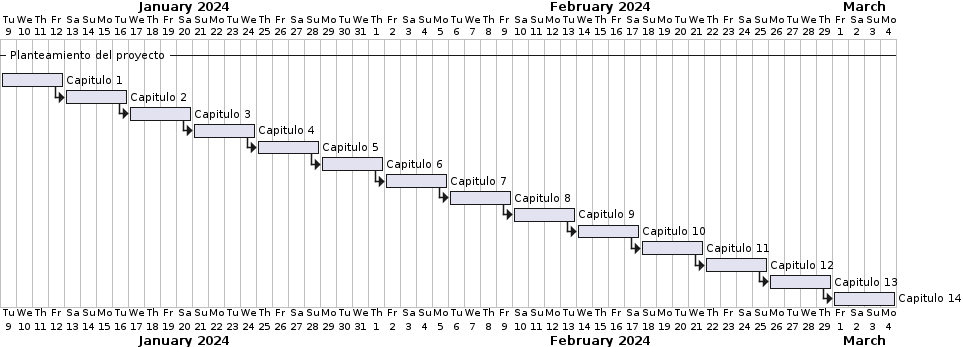
\includegraphics[width=1\linewidth]{figures/chapter01/Gantt.png}
    \caption{Diagrama Gantt}
    \label{fig:gantt}
\end{figure}
% TODO

\subsection{Presupuesto}

% TODO  


\section{Estructura de la memoria}

En este trabajo, hemos utilizado la documentación proporcionada por \textbf{PyTorch} para explicar diversos conceptos de las redes neuronales. Nos referimos a la documentación oficial de PyTorch \cite{pytorch2024github}. Usamos el término \texttt{torch}, \texttt{torch.nn} y \texttt{nn}.

% TODO
\clearpage\thispagestyle{empty}\cleardoublepage

\chapter{ANTECEDENTES Y ESTADO DEL ARTE}
\label{ch:2}
% ====================================================================================== 

\section{Introducción}
\label{ch:2:section:introduction}

El proyecto que desarrollamos se encuentra en una frontera muy difusa de múltiples ramas del conocimiento, siendo muy interdisciplinar, se trata de una revisión de los ataques, seguridad y robustez a las redes neuronales centrándonos en ataques adversariales.
Por lo que debemos explicar que es la ciencia de datos, el proceso \gls{KDD}, la inteligencia artificial generativa y la seguridad informática.

\begin{figure}[H]
    \centering
    \captionsetup{justification=centering}
    \centerline{\includesvg[width=0.75\columnwidth]{figures/ciencia-de-datos.drawio.svg}}
    \caption{Ciencia de datos como campo interdisciplinar.\newline{}Fuente: Elaboración propia}
    \label{fig:ciencia-de-datos}
\end{figure}

Podemos dividir este trabajo en dos secciones muy relacionadas, la primera la inteligencia artificial y de segundo punto de importancia la seguridad de la información.
Desde sus inicios la inteligencia artificial, aunque con buenos resultados en muchos campos de aplicación resultaba en grandes fallos de seguridad, fiabilidad y robustez.
Por cómo están entrenadas las inteligencias artificiales (\acrshort{ANN}) tiene múltiples puntos de ataque que son susceptibles de ser atacados, los principales son los datos, las arquitecturas o los pesos.
Ya que alterando cualquiera de estos componentes de forma se verá enormemente afectada el comportamiento.

% Ciencia de la computación
% minería
% Machine Learning
% Deep Learning
% ANNs
% GANs


\section{Antecedentes}
\label{ch:2:section:background}

% region historia
\subsection{Historia, línea temporal}

%https://www.techtarget.com/searchenterpriseai/tip/The-history-of-artificial-intelligence-Complete-AI-timeline

A continuación, se describe la línea de temporal con los hitos más relevantes en el desarrollo de la inteligencia artificial, sus avances hasta él \gls{DL} y como se ha llegado a las redes neuronales actuales o la inteligencia artificial generativa. Se han adjuntado referencias de las investigaciones, artículos y publicaciones realizadas. \cite{TIMELINE-schmidhuber2022annotated}

Como podemos observar en la línea temporal de la figura \ref{tab:timeline} se realizaron grandes avances en este campo desde principios del siglo \miscrom{XVII}, partiendo de las bases matemáticas como la regla de la cadena, pasando por la teoría Hebbiana hasta nuestros días con los modelos de redes neuronales. Haremos un recorrido de los avances más relevante y su contribución.

Describiremos de forma breve el funcionamiento técnico de los avances más significativos en redes neuronales y visión por computador, para posteriormente explicar las distintas formas de diseñar una red neuronal adversarial generativa.

\begin{table}
    \centering
    \rule{\linewidth}{1pt}
        \ytl{1676     }{The Chain Rule \cite{leibniz2012early}                                                    }
        \ytl{1847     }{Augustin-Louis Cauchy \cite{lemarechal2012cauchy}                                         }
        \ytl{1943     }{Threshold Logic Unit (TLU) \cite{mcculloch1943logical}                                    }
        \ytl{1949     }{Teoría Hebbiana                                                                           }
        \ytl{1958     }{Perceptron \cite{rosenblatt1958perceptron}                                                }
        \ytl{1959-1960}{Adaline y Madaline \cite{rosenblatt1958perceptron}                                        }
        \ytl{1965     }{Multilayer Perceptron (MLP) \cite{baum1988capabilities}                                   }
        \ytl{1967-1968}{Deep Learning by Stochastic Gradient Descent \cite{karplus19671967}                       }
        \ytl{1980`s   }{
            Neuronas Sigmoidales                                            \\
            Feedforward neural network (FNN) \cite{rumelhart1985learning}   \\
            Backpropagation (BP) \cite{rosenblatt1962principles,etde_5080493,lecun1985learning}
        }
        \ytl{1985     }{Boltzmann Machine \cite{ACKLEY1985147}                                                    }
        \ytl{1987     }{Adaptive resonance theory (ART) \cite{grossberg1987competitive}                           }
        \ytl{1989     }{
                        Convolutional neural networks (CNN) \cite{lecun1989backpropagation} \\
                        Recurent neural networks (RNN) \cite{schmidhuber1993habilitation}     
        }
        \ytl{1990     }{Generative Adversarial Networks (GAN) as Game \cite{schmidhuberunsupervised}              }
        \ytl{1997     }{Long short term memory (LSTM) \cite{Hochreiter1997LongSM, hochreiter1997long}             }
        \ytl{2006     }{
            Deep Belief Networks (DBN) \cite{hinton2006fast}            \\
            Restricted Boltzmann Machine \cite{hinton2006reducing}      \\
            Encoder / Decoder (Auto-encoder) \cite{hinton2006reducing}                                
        }
        \ytl{2014     }{Generative Adversarial Networks (GAN) Moderns \cite{6294131,goodfellow2014generative}     }
        \ytl{2018     }{Style Generative Adversarial Networks (Style-GAN) \cite{karras2019stylebased}             }
    \bigskip
    \rule{\linewidth}{1pt}%
    \caption{Hitos de las redes neuronales artificiales}
    \label{tab:timeline}
\end{table}



\newpage
\subsection{Historia de la Inteligencia Artificial}

Todo surge en 1676 por {Gottfried Wilhelm Leibniz} \ref{fig:gottfried-leibniz} publicó la regla de la cadena del cálculo diferencial, esencial para el análisis matemático, es la esencial para calcular como cambiará la función final si se cambian los pesos de funciones anteriores.

La regla de la cadena es fundamental para técnicas como el descenso de gradiente, propuesto por {Augustin-Louis Cauchy} en 1847 y utilizado para ajustar iterativamente los pesos de una \acrshort{NN} durante el entrenamiento.
Posteriormente en 1805 {Adrien-Marie Legendre} y {Johann Carl Friedrich Gauss} desarrollaron \acrshort{NN}, matemáticamente eran regresiones lineales muy simples, similares a las redes neuronales lineales simples.
Esto lo uso {Gauss} para redescubrir el planeta enano Ceres.

\begin{figure}[H]
    \centering
    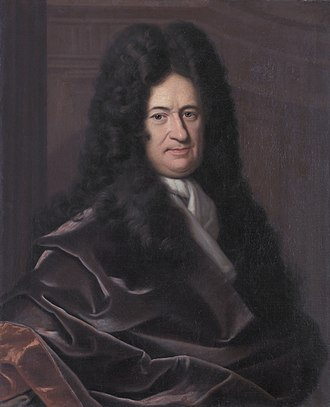
\includegraphics[width=0.45\textwidth]{figures/Gottfried_Wilhelm_Leibniz,_Bernhard_Christoph_Francke.jpg}
    \caption{Retrato de Gottfried Leibniz.\newline{}Fuente: \href{https://es.wikipedia.org/wiki/Gottfried_Leibniz}{Wikipedia}}
    \label{fig:gottfried-leibniz}
\end{figure}

Aunque realmente la historia comienza en 1943 con la investigación de {Warren McCulloch} y {Walter Pitss}, publicaron el artículo \textit{A logical calculus of the ideas immanent in nervous activity} \cite{mcculloch1943logical}.
Dicho artículo creó distintas ramas de investigación (ordenadores digitales, inteligencia artificial, funcionamiento del perceptron).

\begin{figure}[H]
    \centering
    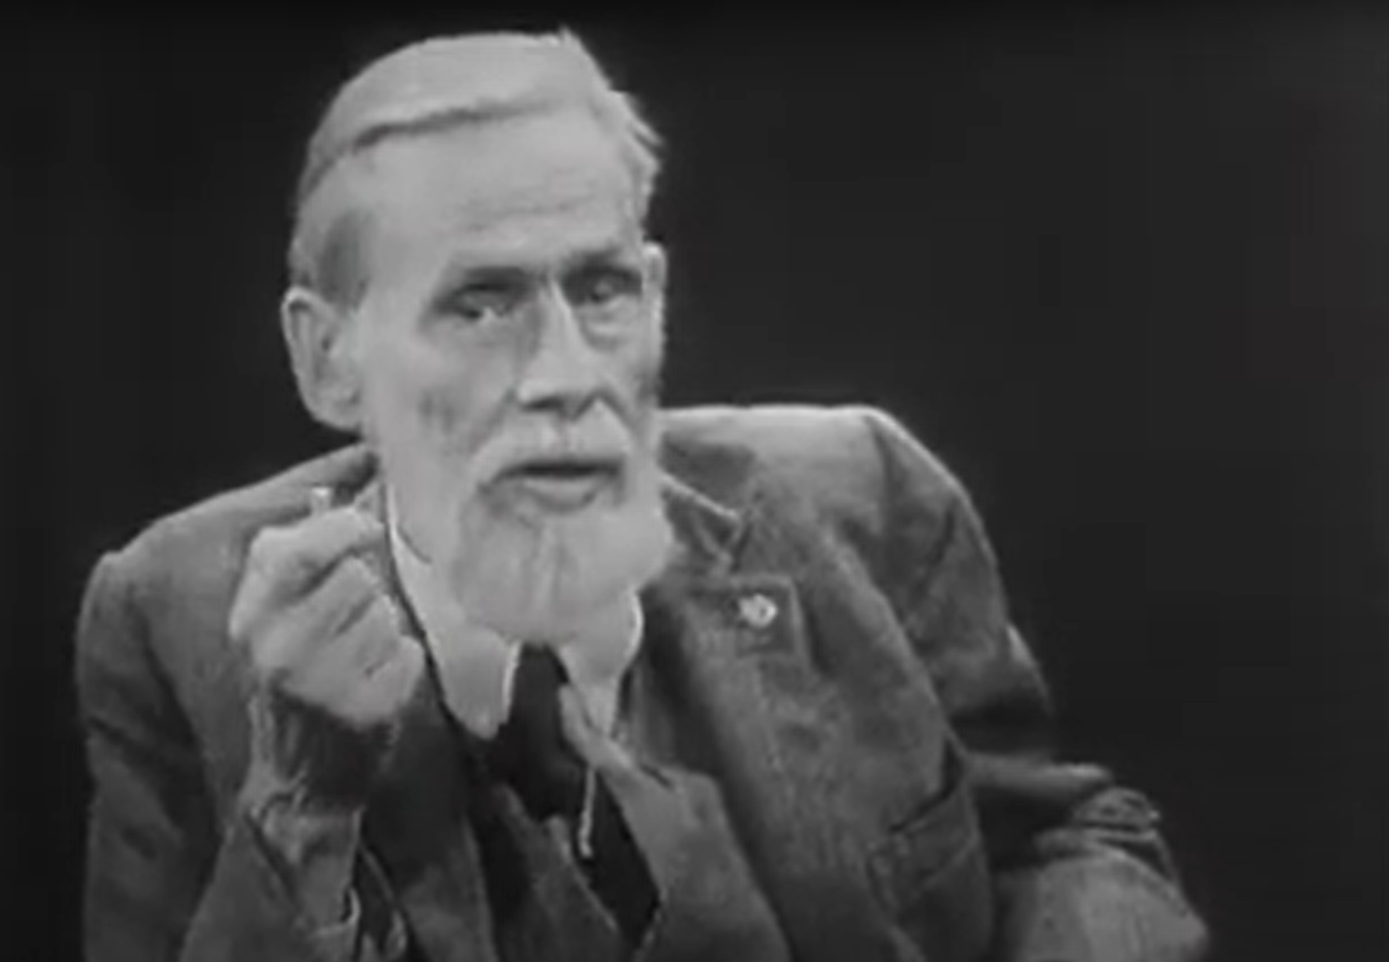
\includegraphics[width=0.55\textwidth]{figures/Warren Sturgis McCulloch Interview.png}
    \caption{Warren Sturgis McCulloch Interview.\newline{}Fuente: \href{https://www.youtube.com/watch?v=8Wdz1Tj5084}{Entrevista en 1969}}
    \label{fig:Warren Sturgis McCulloch}
\end{figure}


En 1956 en la primera conferencia de inteligencia artificial organizada por la fundación {Rochester}, se reúnen los investigadores fundadores de los conceptos actuales de la IA ({Minsky, McCarthy, Rochester, Shanon}), gran parte de la bibliografía se refiere a este punto como el origen y contacto de las redes neuronales artificiales.
En dicha conferencia (\textit{Nathaural Rochester}) presento el modelo de una red neuronal que fue el resultado de la investigación desarrollada por el equipo de investigación de IBM.

\begin{figure}[H]
    \centering
    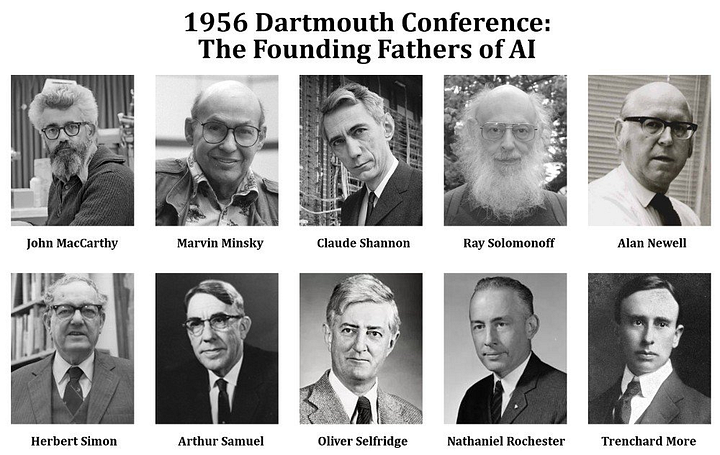
\includegraphics[width=0.75\textwidth]{figures/conferecia 1956 - 1689170718524.png}
    \caption{Los padres de la inteligencia artificial.\newline{}Fuente: \href{https://www.linkedin.com/pulse/first-ever-ai-conference-tracing-evolution-history-ofai-nicky-verd}{Linkedin}}
    \label{fig:conferencia-1956}
\end{figure}

En 1957 se presenta el ``\textit{Perceptron}'' por {Frank Rosenblatt}, dicho elemento es un sistema clasificador de patrones, además contaba con la capacidad de aprender, de ser robusto matemáticamente y poder adaptarse si algún componente se dañaba.

\begin{figure}[H]
    \centering
    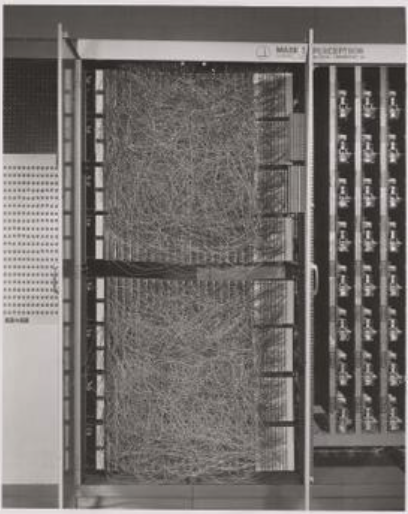
\includegraphics[width=0.4\textwidth]{figures/perceptron.png}
    \caption{Mark I Perceptron.\newline{}Fuente: \href{https://en.wikipedia.org/wiki/Perceptron}{Wikipedia}}
    \label{fig:perceptron}
\end{figure}

El \textit{Perceptron} fue diseñado originalmente para el reconocimiento óptico usando un sistema de 400 fotocélulas en rejilla.
Posteriormente, se describió el problema de no-linealidad que presentaban los perceptrones (Problema XOR) \cite{cuevastello2018apuntes}.

De 1959 a 1960 {Bernard Widrow} y {Ted Hoff} desarrollaron ``Adaline'' y ``Madaline'' \cite{widrow1960adaptive} que resolvía el problema de la no-linealidad y que tenía aplicación en el reconocimiento de voz, series temporales, caracteres, etc.

Posteriormente, el \textit{MIT} realizo una investigación matemática muy crítica de todos los problemas que presentaba el \textit{Perceptron} llegando a la conclusión que tenían grandes problemas que no podrían ser resueltos, por lo que en la próxima década (años 60) se redujo drásticamente las investigaciones sobre el campo de las redes neuronales.
Esto llevo a uno de los famosos inviernos de la inteligencia artificial (1974 - 1980).

\begin{figure}[H]
    \centering
    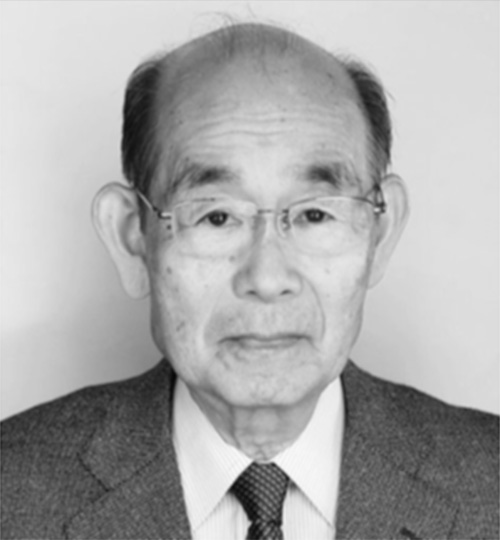
\includegraphics[width=0.25\textwidth]{figures/Kunihiko Fukushima.jpg}
    \caption{Kunihiko Fukushima.\newline{}Fuente: \href{https://www.ieice.org/eng/about_ieice/new_honorary_members_award_winners/2017/meiyo_05e.html}{IEICE}}
    \label{fig:kunihiko-fukushima}
\end{figure}

Durante la década de los 70 se hacen aportes a la teoría \textit{Hebbiana}, se aportan logros en al análisis y descripción de reglas adaptativas, además de otros aportes al principio de aprendizaje competitivo.
En 1979 presentó {Kunihiko Fukushima} la primera red neuronal \gls{CNN}, la llamó Neocognitron \cite{fukushima1979neural}, dicho trabajo en un futuro se mejoraría con técnicas de \gls{BP-NN}.

En la década de los 80 se realizaron aportes como el algoritmo de \gls{BP-NN} que surgió del artículo de {Hopfield} \cite{hopfield1982neural}, esto despertó la curiosidad de muchos investigadores a volver al campo de las redes neuronales.
Se realizaron aportes como las redes \gls{GNN}.
La investigación continuó con {Stephen Grossberg} que realizo aportes derivados de estudios fisiológicos de cómo funcionaban las neuronas y la plasticidad, lo que permitió la creación de reglas y postulados, esto se ve en los trabajos de las redes \acrshort{ART-NN} \cite{grossberg1987competitive}.
La investigación de {Hopfield} basada en el trabajo de {Stephen Grossberg} creo un sistema computacional neuronal interconectado que tiende a un mínimo de energía.
En 1985 {David E. Rumelhart} basándose en la investigación realizada por {Paul Werbos} \cite{etde_5080493} realizo un análisis experimental del algoritmo \gls{BP-NN} y su aplicación en redes \acrshort{FNN} \cite{rumelhart1985learning}.

{Yann LeCun} junto a su equipo, en 1989 crearon la primera aplicación \acrshort{CNN} con técnicas \acrshort{BP} dicha aplicación podía reconocer números a partir de imágenes.

\begin{figure}[H]
    \centering
    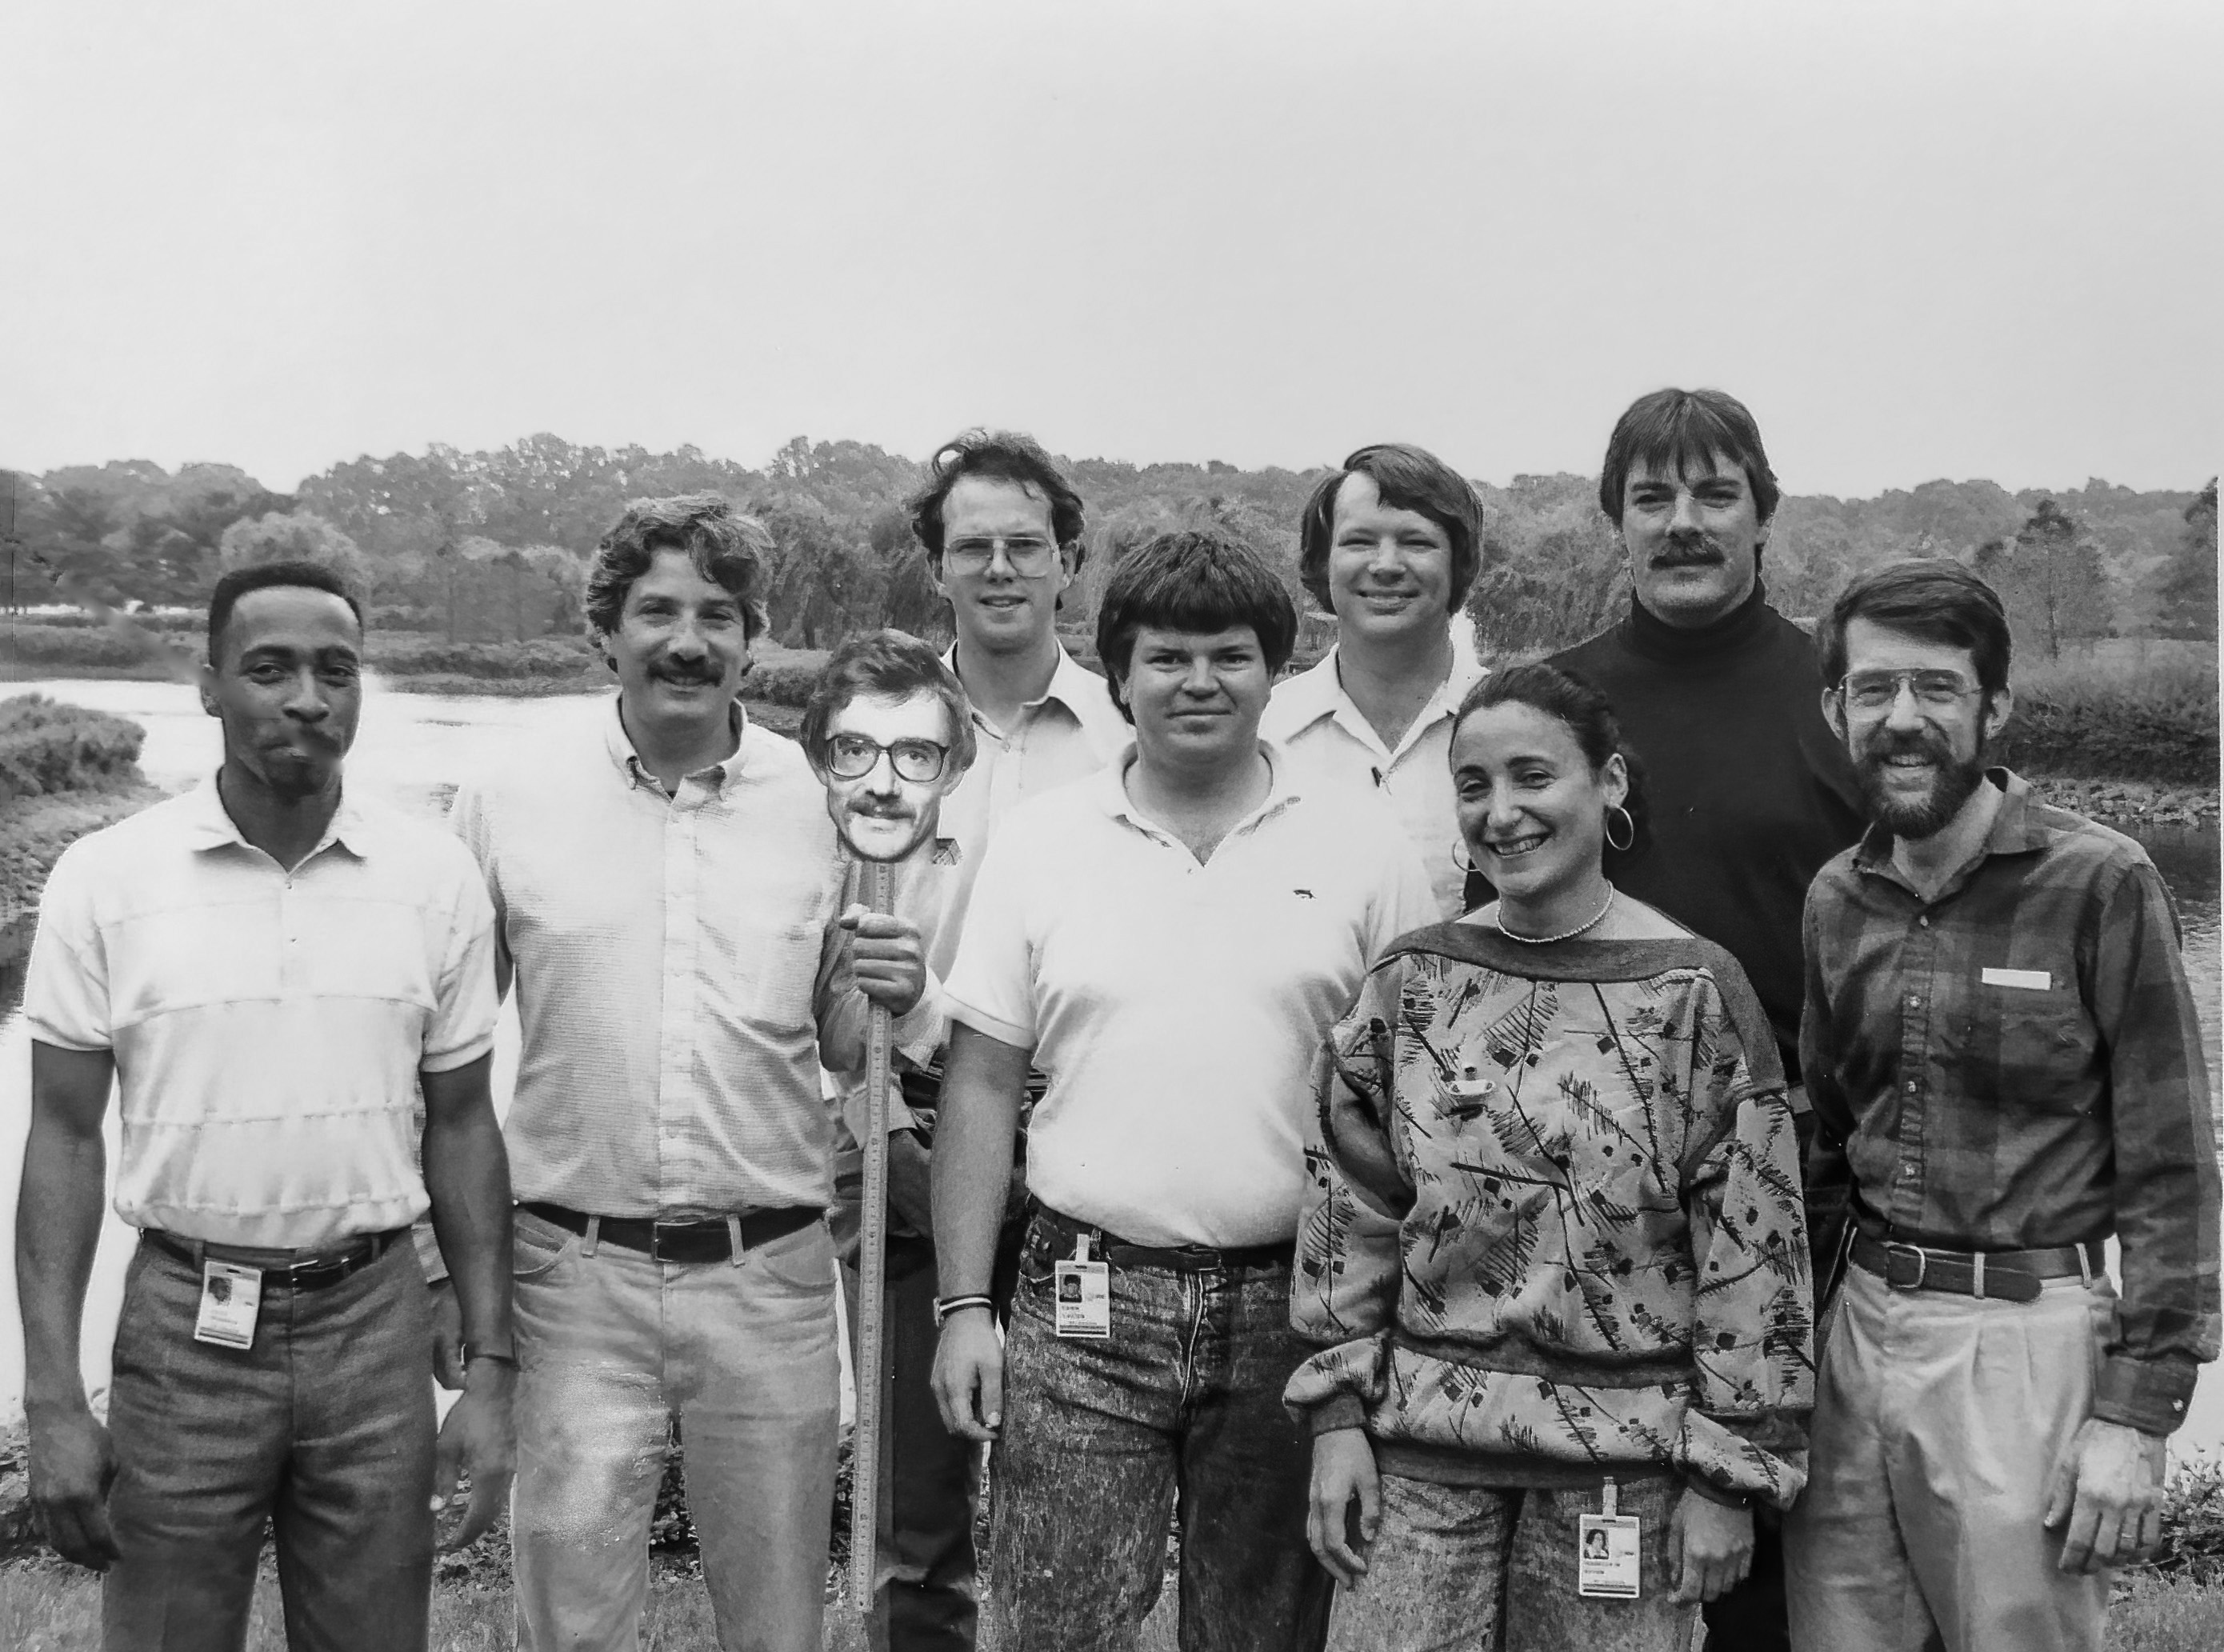
\includegraphics[width=0.65\textwidth]{figures/yann-lecun - EyIwmEDW8AIQs1C.jpeg}
    \caption{Adaptive Systems Research Department at Bell Labs 1989.\newline{}Fuente: \href{https://twitter.com/ylecun/status/1378718317695934465}{Twitter Yann Lecun}}
    \label{fig:adaptive-systems-research-department-at-bell-labs}
\end{figure}

En la década de los 90 se presentaron múltiples investigaciones y muchos avances en el campo, uno de los más importantes fue la presentación de la primera \acrshort{GAN} como una curiosidad, ya que se presentó como un duelo entre dos redes neuronales, en un principio fue un generador probabilístico y un predictor con el objetivo de maximizar la pérdida de cada uno en un juego \textit{minimax}.

En 1991 se presentó el trabajo \textit{Predictability Minimization} \cite{urgen1991learning} dichas técnicas sirvieron de inspiración para el aprendizaje por refuerzo,
En marzo de 1991 se hizo una aproximación a los \textit{transformers} con auto atención, lograron separar el conocimiento del control como una máquina clásica, pero de una forma completamente neuronal, además de gestionar actualizaciones de los pesos de forma muy rápida y eficiente.

Durante la década de 1990 las redes neuronales tendían a ser muy sencillas, con pocas capas y no muy complejas por las limitaciones técnicas de la época.
Por lo que muchos investigadores propusieron soluciones similares a las redes \acrshort{RNN} que permitían una retroalimentación, además de aceptar secuencias de información arbitraria.
Otros propusieron soluciones como la jerarquía de \acrshort{RNN} autosupervisada que aprende representaciones en distintos niveles de abstracción.
Comienzan a proponerse redes similares a las que en un futuro se llamarían \acrshort{DBN} como un método no supervisado para \acrshort{FNN}.

En junio de 1991 {Sepp Hochreiter} Figura \ref{fig:sepp-hochreiter} implemento el primer compresor de redes neuronales, además demostró uno de los principales problemas de las \acrshort{NN} el llamado problema del desvanecimiento o explosión del gradiente \ref{sec:gradient-descent} que hacía que el aprendizaje fallará.
Un análisis posterior condujo a los investigadores a una primera aproximación \acrshort{LSTM}, aunque no sería hasta 1997 con la revisión por pares y publicación del artículo \textit{Long short-term memory} \cite{hochreiter1997long} que se solucionaría parcialmente el problema.

\begin{figure}[H]
    \centering
    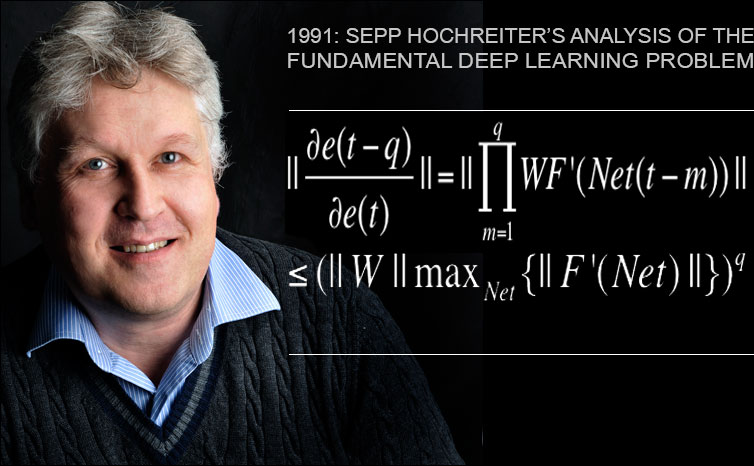
\includegraphics[width=0.65\textwidth]{figures/Sepp Hochreiter.jpg}
    \caption{Sepp Hochreiter.\newline{}Fuente: \href{https://people.idsia.ch/~juergen/fundamentaldeeplearningproblem.html}{IDSIA}}
    \label{fig:sepp-hochreiter}
\end{figure}

Más adelante, en el 2014 {Goodfellow} Figura \ref{fig:gan-ian-goodfellow} presento la primera red neuronal \gls{GAN} pura para la generación de imágenes mediante el enfrentamiento de una red neuronal generativa contra una red neuronal discriminante entrenadas con el mismo conjunto de datos \cite{goodfellow2014generative}.
Durante los próximos años se realizaron muchos aportes a las redes neuronales generativas, principalmente de paralelización de los cálculos, técnicas de estabilización, generación condiciona, arquitecturas más eficientes, funciones de pérdidas más adecuadas, aplicaciones específicas (cambiar el estilo de pintura), redes apiladas, etc.
Fruto de todo ello, {NVIDIA} en 2018 presento \gls{StyleGAN} \cite{karras2019stylebased} un modelo que es capaz de crear imágenes sintéticas de alta calidad y resolución, publicando el código en 2019 con mejoras relevantes a su primera versión.

\begin{figure}[H]
    \centering
    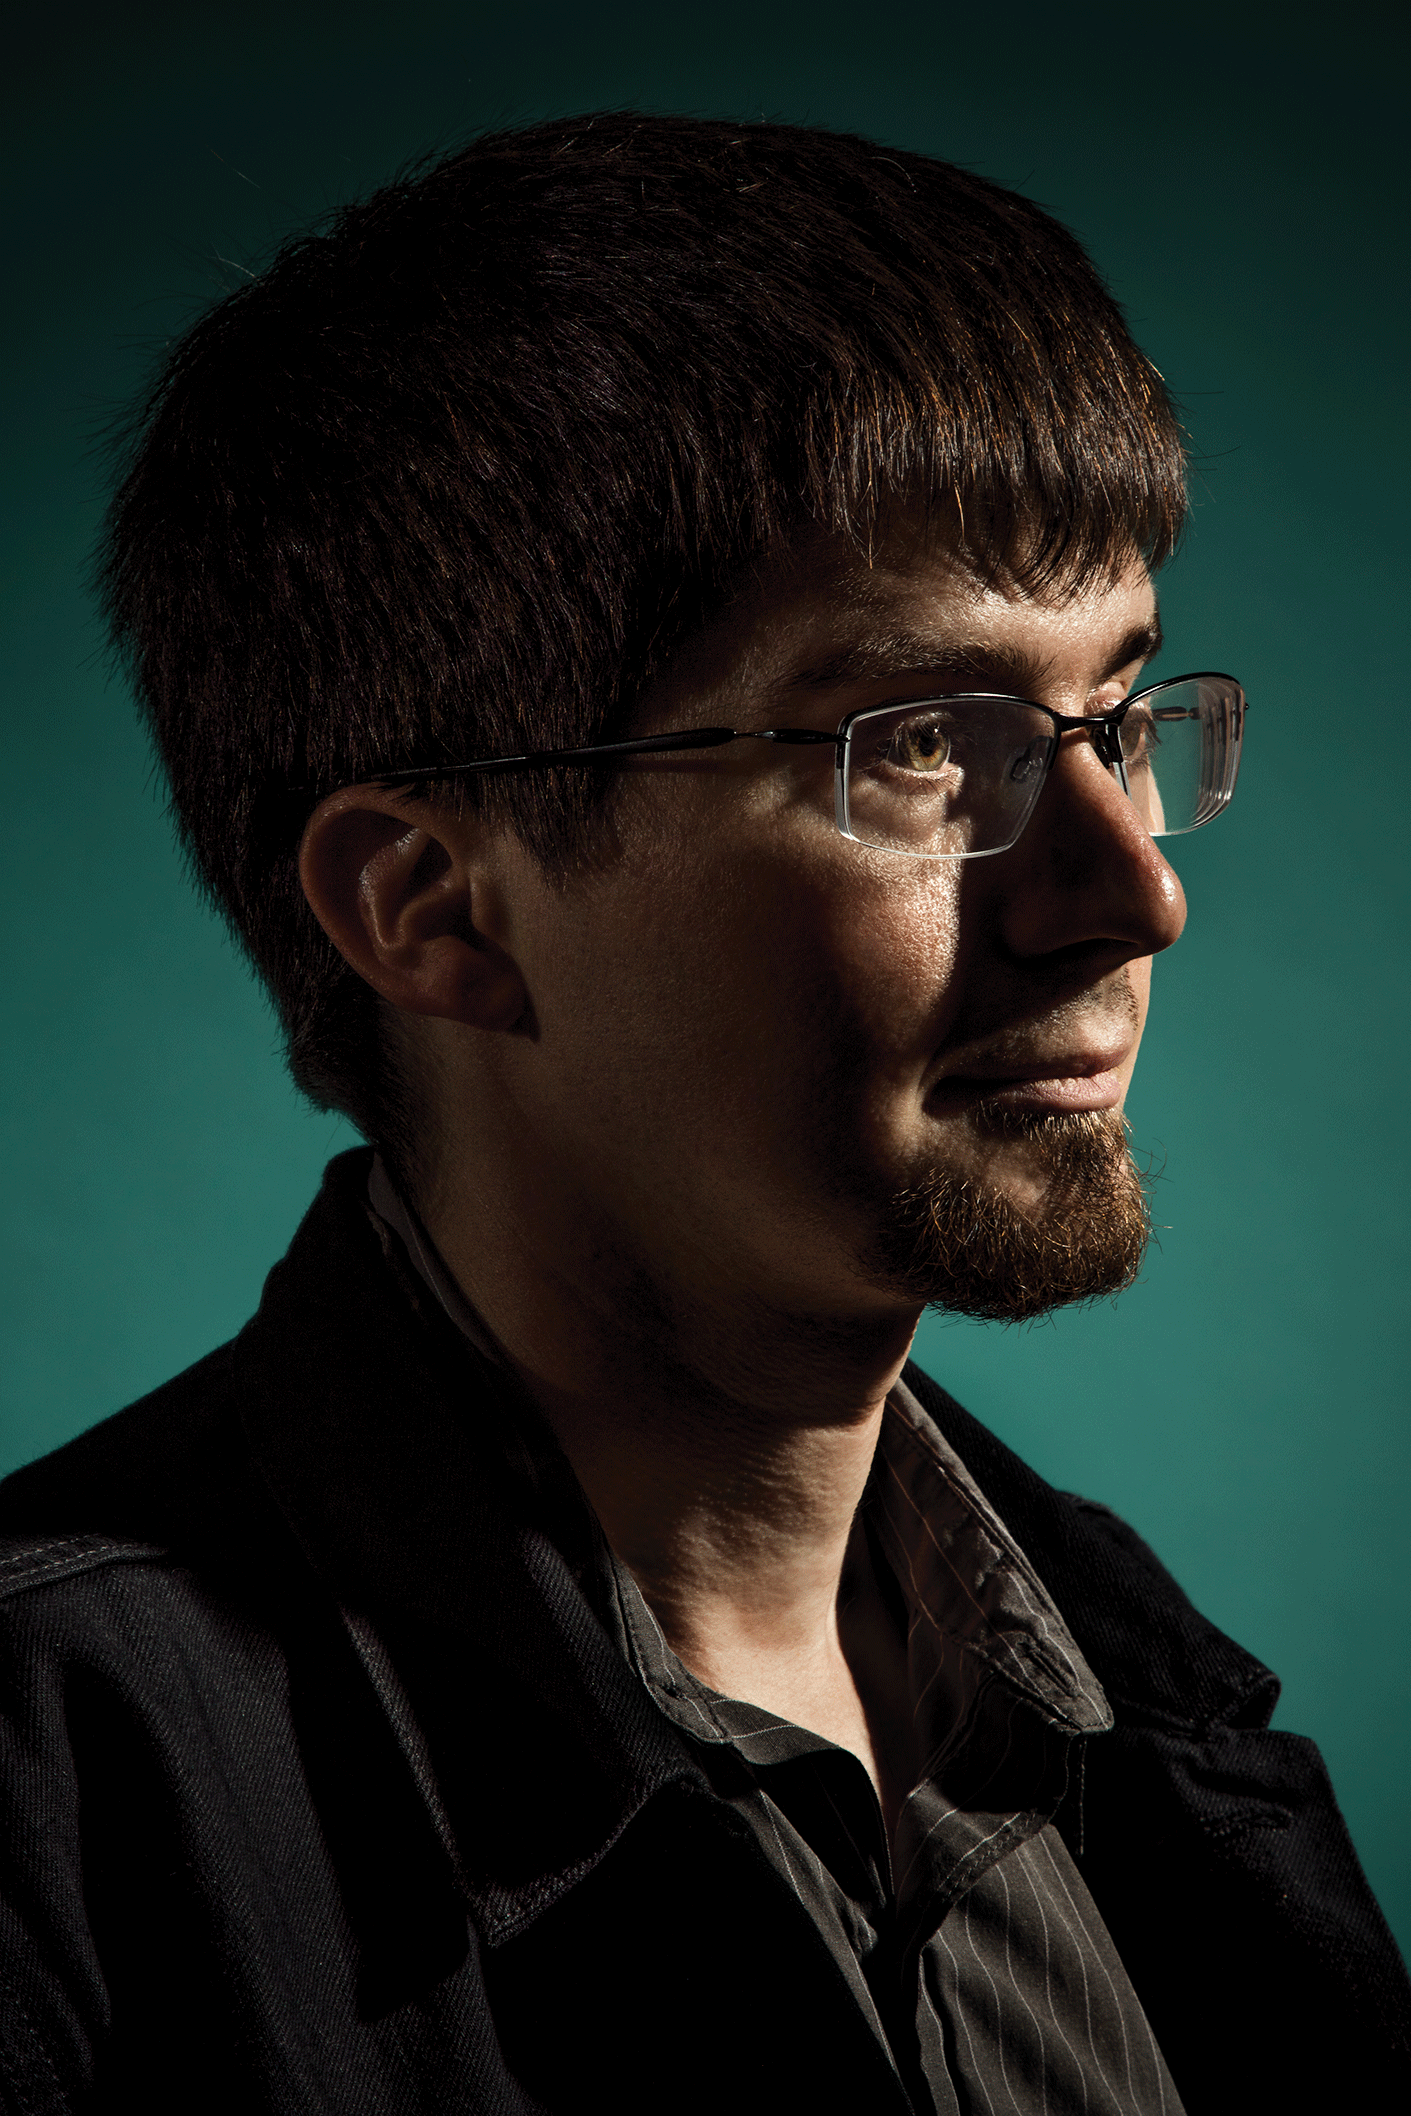
\includegraphics[width=0.2\textwidth]{figures/gan-goodfellow.png}
    \caption{Ian Goodfellow.\newline{}Fuente: \href{https://www.technologyreview.es/s/10016/el-senor-de-las-gan-el-hombre-que-dio-imaginacion-las-maquinas}{MIT Technology Review}}
    \label{fig:gan-ian-goodfellow}
\end{figure}
% endregion


\section{Estado del arte}
\label{ch:2:section:state-of-the-art}

\subsection{La ciencia de datos}
% region subsection La ciencia de datos

La ciencia de datos (\textit{Data Science}) es el estudio de los datos con el objetivo de extraer información útil, se usa principalmente para dar información útil a empresas. Es un campo multidisciplinar, ya que combina campos de las matemáticas, estadística e inteligencia artificial para analizar grandes cantidades de datos. Esto tiene como objetivo responder a las siguientes cuestiones: \textit{¿Qué paso?, ¿Por qué pasó?, ¿Qué pasará? O ¿Qué se puede hacer con los resultados?} \cite{aws-data-science}

La ciencia de datos analiza los datos de distintas formas.

\begin{enumerate}
    \item \textbf{Análisis descriptivo}: examina datos con visualizaciones (gráficos, tablas) para entender eventos pasados o actuales.
    \item \textbf{Análisis de diagnóstico}: profundiza en los datos para entender las razones detrás del evento. Emplea técnicas como descubrimiento de datos o correlaciones.
    \item \textbf{Análisis predictivo}: utiliza datos históricos y técnicas como machine learning para hacer predicciones precisas sobre patrones futuros.
    \item \textbf{Análisis prescriptivo}: busca la mejor respuesta para un resultado esperado. Utiliza técnicas como simulación y redes neuronales para recomendar el mejor curso de acción entre varias alternativas.
\end{enumerate}

% endregion subsection La ciencia de datos

\subsection{La minería de datos}
% region subsection La minería de datos
% Fases de la extracción del conocimiento 
% Dentro del KDD está la {minería de datos}

La minería de datos, es una técnica asistida por computadora, procesa grandes conjuntos de datos para descubrir patrones y relaciones ocultas. Este conocimiento resultante se aplica en la resolución de problemas, análisis de decisiones empresariales, etc. Esta técnica tiene distintas fases para procesar y extraer información útil.

\begin{enumerate}
    \item Comprender, identificar y definir el alcance del proyecto.
    \item Comprender los datos.
    \item Depurar datos (limpiar, integrar y dar formato).
    \item Modelar datos.
    \item Evaluar los resultados.
    \item Implementar resultados.
\end{enumerate}

La minería de datos es distinta en función de los datos y el objetivo, la mayoría del estado del arte segmenta la minería en tres tipos, minería de procesos, minería de textos y minería predictiva.

El Descubrimiento de Conocimientos en Bases de Datos \gls{KDD} es un proceso que utiliza algoritmos de minería de datos para explorar y extraer conocimientos útiles de grandes bases de datos. Con el avance tecnológico, se emplean técnicas de inteligencia artificial para este propósito, con el objetivo final de obtener conocimiento de alto nivel a partir de datos de bajo nivel. La Figura \ref{fig:kdd} esquematiza el proceso general del \textit{KDD}.

\begin{figure}[H]
    \centering
    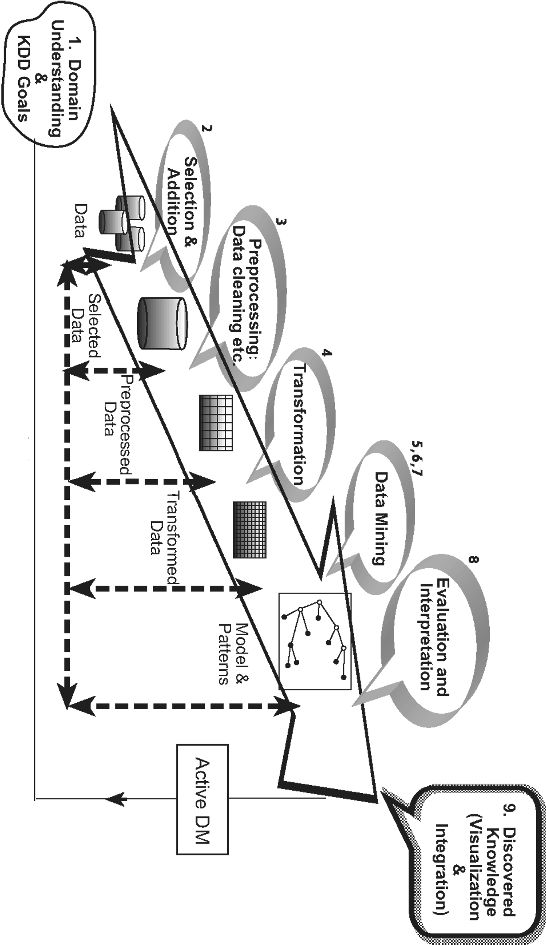
\includegraphics[angle=90,width=0.8\textwidth]{figures/chapter02/KDD.jpg}
    \caption{El proceso de descubrimiento de conocimiento en bases de datos.\newline{}Fuente: Sección \textit{Introduction to Knowledge Discovery and Data Mining} \cite{rokach2010data}}
    \label{fig:kdd}
\end{figure}

\begin{enumerate}
    \item \textbf{Comprensión del Dominio de Aplicación}: se debe comprender los datos que se tratan y el campo de obtención con el objetivo de preparar los datos.
    \item \textbf{Selección y Creación de Conjunto de Datos}: se han de seleccionar los datos relevantes (Selección de características).
    \item \textbf{Preprocesamiento y Limpieza de Datos}: se han de eliminar las características no relevantes, datos perturbados, entradas incoherentes o tratar datos faltantes, etc. con el objetivo de obtener datos más limpios.
    \item \textbf{Transformación de Datos}: se deben tratar los datos, reduciendo la dimensionalidad, filtración, descomponiendo, etc. para que sea más sencillo el consumo de estos datos por una aplicación.
    \item \textbf{Elección de Tarea de Minería de Datos}: en función de los datos y del objetivo deberemos realizar una tarea (clasificación, regresión o agrupación), ya que en la minería de datos hay dos objetivos principales, \textbf{predicción} y \textbf{descripción}.
    \item \textbf{Elección del Algoritmo de Minería de Datos}: deberemos elegir entre los distintos algoritmos que se usan en la minería de datos, si buscamos precisión podemos usar redes neuronales, si buscamos explicabilidad podemos usar árboles de decisión.
    \item \textbf{Implementación del Algoritmo de Minería de Datos}: emplearemos el algoritmo seleccionado ajustando los parámetros para que nos del mejor resultado.
    \item \textbf{Evaluación de Patrones Minados}: debemos interpretar los resultados (reglas, confiabilidad, etc.) si no cumplen los objetivos que se buscaban en el primer paso deberemos reajustar toda la metodología, desde ajustar la selección de características a la interpretación o compresibilidad del modelo.
    \item \textbf{Utilización del Conocimiento Descubierto}: por último, debemos incorporar el conocimiento a los sistemas de toma de decisiones, este es el paso más importante, ya que con él podemos medir los efectos del conocimiento obtenido. Puede suceder que una vez implementado el modelo en sistema de producción pierda eficiencia si las condiciones reales son distintas a las de la creación del modelo.
\end{enumerate}

\begin{figure}[H]
    \centering
    \centerline{\includesvg[width=1\linewidth]{figures/chapter02/data-mining-taxonomy.drawio.svg}}
    \caption{Taxonomía de minería de datos.\newline{}Fuente: Elaboración propia, inspirado en la sección \textit{Introduction to Knowledge Discovery and Data Mining} \cite{maimon2005data}}
    \label{fig:data-mining-taxonomy}
\end{figure}

La minería de datos puede estar orientada a la verificación o al descubrimiento de patrones, se debe automatizar su identificación, pudiendo usar un enfoque predictivo o descriptivo. Para el descubrimiento se usa el aprendizaje inductivo, mientras que en el paso de verificación se ha de evaluar las hipótesis externas usando métodos estadísticos clásicos. La terminología clásica del aprendizaje automático está clasificado en supervisado (clasificación y regresión) y no supervisado (agrupamiento), aunque existen muchos más términos en la terminología moderna esto podemos analizarlo más en profundidad en el libro \textit{Data Mining and Knowledge Discovery Handbook} \cite{maimon2005data}.

% endregion subsection La minería de datos

\subsection{Aprendizaje automático - \textit{Machine Learning}}
% region subsection Aprendizaje automático

El \textit{machine learning} es la ciencia o rama de la inteligencia artificial que desarrolla, modelos estadísticos, desarrolla algoritmos que generalizan comportamientos y reconocen patrones. Es decir, hace posible el aprendizaje autónomo de las máquinas para realizar tareas sin la necesidad programar las instrucciones explícitamente. El \textit{machine learning} busca procesar grandes cantidades de datos e identificar patrones de datos de forma automática.

\begin{figure}[H]
    \centering
    \centerline{\includesvg[width=0.75\linewidth]{figures/chapter02/machine-learning-rules.drawio.svg}}
    \caption{El \textit{Machine Learning} como paradigma de programación.\newline{}Fuente: Elaboración propia}
    \label{fig:machine-learning-rules}
\end{figure}

Como podemos ver en la Figura \ref{fig:machine-learning-rules} en el paradigma clásico se necesitaba conocer el dominio de los datos y las reglas en profundidad y programar los descriptores de forma manual para procesar los datos. En el paradigma del \textit{machine learning} permite extraer esas reglas y patrones para procesar nuevos datos a partir de respuestas que conocíamos previamente, estas respuestas previas deben ser extraídas o validadas por expertos.

Una clasificación de las tareas del \textit{machine learning} lo podemos ver en la Figura \ref{fig:machine-learning}, esta clasificación está dividida en función de cómo se realiza el aprendizaje del modelo.

\begin{figure}[H]
    \centering
    \centerline{\includesvg[width=1\linewidth]{figures/chapter02/machine-learning.drawio.svg}}
    \caption{Clasificación de los algoritmos de aprendizaje automático.\newline{}Fuente: Elaboración propia}
    \label{fig:machine-learning}
\end{figure}

El \textit{machine learning} puede trabajar con datos estructurados y no estructurados, aunque estos últimos requieren un procesamiento previo para adaptarlos en un formato estructurado.

% endregion subsection Aprendizaje automático

\subsection{Aprendizaje profundo - \textit{Deep Learning}}
% region subsection Aprendizaje profundo
% TODO: Explicar el Deep Learning 
% https://idus.us.es/bitstream/handle/11441/90004/Centeno%20Franco%20Alba%20TFG.pdf
% https://learning.oreilly.com/library/view/neural-networks-and/9781492037354/ch01.html#idm139624964652336

El \textit{deep learning} es una rama del \textit{machine learning} que usa redes neuronales artificiales para analizar datos no lineales, estas redes imitan el comportamiento del cerebro humano, para esto suelen contar con arquitecturas complejas.
Se distingue del \textit{machine learning} por los tipos de datos con los que puede trabajar y por los métodos con los que hace que los modelos aprendan.

Otra de las características que diferencia al \textit{deep learning} del \textit{machine learning} es que elimina parte del procesamiento previo de datos, ya que sus algoritmos pueden ingerir y procesar datos no estructurados.


% endregion subsection Aprendizaje profundo
\subsection{Redes neuronales artificiales - \textit{Artificial Neuronal Networks}}
% region subsection Redes neuronales artificiales
% TODO: \cite{ibm-deep-learning}
% Explicar uso de múltiples neuronas artificiales para crear capas y luego redes
El \textit{deep learning} emplea principalmente redes neuronales para reconocer, clasificar y describir con precisión patrones de datos. Estas redes están inspiradas en el funcionamiento del cerebro humano.  \cite{ibm-deep-learning}

Las redes neuronales es un conjunto de neuronas artificiales que están organizadas generalmente por capas. Estas redes tienen una capa de entrada, una capa de salida y múltiples capas ocultas con distintas funciones de activación que ponderan los pesos de cada neurona.

Existen formas muy variadas de componer las capas, a esto se le denomina \textbf{topología de red neuronal}, en función del objetivo que se busque, la topología será muy distinta.

\subsubsection{Elementos de una neurona artificial}
% region subsubsection Elementos de una neurona artificial
% TODO explicar las partes que propusieron \textit{McCulloch} y \textit{Pitts}

Como se ha comentado previamente las neuronas artificiales están inspiradas en las neuronas biológicas del cerebro humano, fueron los investigadores \textit{McCulloch} y \textit{Pitts} \cite{mcculloch1943logical} los que sentaron las bases de lo que es una neurona artificial, demostrando que su modelo de red neuronal podía realizar cálculos que se correspondían con la lógica proposicional.


\begin{figure}[H]
    \centering
    \centerline{\includesvg[width=1\linewidth]{figures/chapter02/artificial-neuron.drawio.svg}}
    \caption{Partes de una neurona artificial bioinspirada en una neurona biológica.\newline{}Fuente: Elaboración propia}
    \label{fig:artificial-neuron}
\end{figure}

En la Figura \ref{fig:artificial-neuron} podemos ver las distintas partes de una única neurona artificial y sus partes equivalentes con una neurona biológica. El axón opera como la entrada de información a la neurona. La sinapsis como las conexiones con la neurona que son los pesos. El cuerpo celular como la unidad de procesamiento central, donde se pondera la suma de las señales de entrada. El cuello del axón sería nuestra función de activación que se activa cuando supera un umbral. Y por último el axón sería nuestra señal de salida.



% perceptron simple
% perceptron multicapa
% Funciones de optimización
% Funciones de activación
% Funciones de perdida
% CapasThe next payment of €9.68 will be collected on March 13th, 2024 10:26 AM UTC.

% Tipologías
% Descenso de gradiente

% endregion subsubsection Elementos de una neurona artificial

\subsubsection{Funcionamiento de una red neuronal} \label{neural-network}
% region subsubsection Funcionamiento de una red neuronal

Las redes neuronales profundas tienen multitud de capas con nodos interconectados, cada capa sobre la capa anterior con el objetivo de optimizar la precisión de una perdición o clasificación. A esta progresión de cálculos se le denomina ``propagación hacia delante''.

El proceso de ``propagación inversa'' es el encargado de calcular errores de precisión, ajustar sesgos y ponderaciones usando algoritmos como \nameref{sec:gradient-descent}.

La capa de entrada es por donde el modelo ingiere los datos, y la capa de salida es donde el modelo responderá con la predicción o clasificación una vez se haya completado la fase de aprendizaje.

\begin{figure}[H]
    \centering
    \centerline{\includesvg[width=1\linewidth]{figures/chapter02/neuronal-network.drawio.svg}}
    \caption{Red neuronal artificial.\newline{}Fuente: Elaboración propia}
    \label{fig:artificial-neuronal-network}
\end{figure}

En la Figura \ref{fig:artificial-neuronal-network} podemos ver una arquitectura simple de una red neuronal que cuenta con la capa de entrada, la capa de salida y dos capas ocultas.

El vector de entrada ${X = (x_{1}, x_{2}, ..., x_{n})}$ será la información suministrada a nuestra red a través de la capa de entrada, este vector será de tamaño ${n}$.

\begin{figure}[H]
    \centering
    \captionsetup{justification=centering}
    \centerline{\includesvg[width=1\linewidth]{figures/equations/Notation.drawio.svg}}
    \caption{Cálculo de los pesos de la red neuronal artificial.\newline{}Fuente: Elaboración propia}
    \label{fig:notation}
\end{figure}

\begin{enumerate}
    \item Función de la red neuronal: ${f(x) = W x + b}$
    \item Matriz de pesos: ${W = \left[w_{0,n}, w_{1,n}, ...,w_{m,n}\right]}$
    \item Vector de pesos: ${w_{n} \in \mathbb{R}^{D}}$
    \item Vector de entrada: ${x \in \mathbb{R}^{D}}$
    \item Vector del bias: ${b \in \mathbb{R}^{C}}$
\end{enumerate}

% El proceso de reducción de dimensionalidad se lleva a cabo, para convertir el vector de características del espacio original en un nuevo espacio con un conjunto más pequeño, linealmente no correlacionadas mediante la siguiente función $f: \mathbb{R}^{D} \rightarrow \mathbb{R}^{C}$ con $C \ll D$, donde la red neuronal está expresada como $f(x) = W x + b$. Esta red cuenta con las siguientes partes $\mathbf{W} = \left[w_{0}^{T}, w_{1}^{T}, \cdots, w_{C}^{T}\right]$ es la matriz de vectores de peso, que viene dada la expresión $\mathbf{w_{j}} \in \mathbb{R}^{D}$. El vector de entrada es $\mathbf{x} \in \mathbb{R}^{D}$ y el $bias$ es un vector que está definido en el espacio $\mathbf{b} \in \mathbb{R}^{C}$

\paragraph*{El perceptrón simple}
% TODO: Definición
% TODO: Usos 
% TODO: Algoritmo de entranmiento
% TODO: Problema XOR

El Perceptron es una neurona artificial simple llamada también como \gls{LTU}. La \gls{LTU} calcula una suma ponderada de los valores de las entradas, ${Z = w_{1} x_{1} + w_{2} x_{2} + \cdots + w_{n} x_{n}}$ se aplica el umbral para generar el resultado.

La función umbral común en \gls{LTU} es la función Heaviside \ref{eq:heaviside}.

\noindent\begin{minipage}{0.45\textwidth}
    \begin{equation*}
        heaviside(z) =
        \begin{cases}
            0 & \textup{si } z < 0       \\
            1 & \textup{si } z \geq{}  0
        \end{cases}
    \end{equation*}
\end{minipage}
\begin{minipage}{0.45\textwidth}
    \begin{equation}
        sgn(z) =
        \begin{cases}
            -1 & \textup{si } z < 0  \\
            0  & \textup{si } z = 0  \\
            +1 & \textup{si } z >  0
        \end{cases}
        \label{eq:heaviside}
    \end{equation}
\end{minipage}

Se puede emplear para una clasificación binaria lineal simple, mediante una combinación lineal de las entradas; si la operación supera el umbral, se obtendrá un resultado binario en un vector.

El algoritmo de entrenamiento del perceptrón se basa en ajustar los pesos de conexión entre las entradas y la neurona de salida para mejorar la precisión de las predicciones. Está inspirado en la regla de Hebb, que sugiere que las conexiones entre neuronas se fortalecen cuando una neurona activa repetidamente a otra.

Primero inicializa los pesos, predice, evalúa su error y actualización de los pesos para en la siguiente iteración minimizar su error.

Rosenblatt demostró que el algoritmo convergería hacia una solución, esto es llamado el Teorema de convergencia del perceptrón \cite{geron2018neural}.

Marvin Minsky y Seymour encontraron una serie de debilidades que los perceptrones son incapaces de resolver, algunas de estas debilidades se pueden resolver apilando varios perceptrones, la \acrshort{ANN} resultante se le llama \gls{MLP}.

Uno de los problemas clásicos que tenían los perceptrones simples era el problema de clasificación XOR, esto está representado en la Figura \ref{fig:problem-xor}. Como tal, el perceptrón es un modelo que puede aprender funciones lineales, pero el problema XOR no es linealmente separable, lo que significa que no se puede trazar una línea recta para separar las dos clases (A y B) en el espacio de entrada binario de dos dimensiones.

\begin{figure}[H]
    \centering
    \centerline{\includesvg[width=0.35\linewidth]{figures/chapter02/tfm-xor-problem.drawio.svg}}
    \caption{Problema de clasificación XOR.\newline{}Fuente: Elaboración propia}
    \label{fig:problem-xor}
\end{figure}


\paragraph*{El perceptron multicapa y retropropagación}

Fue en 1986 cuando {D. E. Rumelhart} propuso la retro propagación junto a múltiples capas para resolver el problema de clasificación XOR.

El proceso es el siguiente, por cada instancia de entrenamiento se calcula la salida de cada neurona en la capa consecutiva (paso hacia adelante). A continuación se mide el error de salida de la red (la diferencia entre la salida deseada y la de la red) calculará cuánto contribuyo cada neurona en la última capa oculta al error de cada neurona de salida. Se mide cuantas contribuciones de error provienen de cada neurona en la capa oculta anterior, así sucesivamente hasta que se llega a la capa de entrada(paso hacia atrás). Se mide eficientemente el gradiente de error en todos los pesos de la conexión en la red propagando el gradiente de error hacia atrás. \cite{geron2018neural}

Este proceso funciona, ya que se cambió la función escalonada de las \gls{LTU} a una función logística Sigmoid, esto se requería, ya que la función de paso contiene solo segmentos planos y, por tanto, no había gradientes. Esto permitió que el descenso de gradiente pudiera ir progresando lentamente hasta converger. El algoritmo de retroalimentación se puede usar con otras funciones de activación que veremos más adelante.

% endregion subsubsection Funcionamiento de una red neuronal

\subsubsection{El descenso de gradiente} \label{sec:gradient-descent}
% region El descenso de gradiente
% README: https://www.ibm.com/mx-es/topics/gradient-descent
% TODO: definición
% TODO: como funciona 
% TODO: tipos de descenso
% TODO: desafios (problema)

El método de descenso de gradiente trata de encontrar un mínimo en una función dada, ya sea local o global. El método usa el gradiente negativo ${-\nabla{f}}$, con este método obtenemos la dirección con el descenso máximo en los valores de la función, con esto buscamos encontrar la posición mínima.

En términos simples, el descenso de gradiente va ajustando iterativamente los valores de los parámetros en la dirección opuesta al gradiente de la función de costo. Al moverse en la dirección opuesta al gradiente, el algoritmo busca alcanzar el mínimo local o global de la función de costo.

\begin{figure}[H]
    \centering
    \centerline{\includesvg[width=0.6\linewidth]{figures/chapter02/fx_optimizer.svg}}
    \caption{Descenso de gradiente.\newline{}Fuente: \href{https://fxdatalabs.com}{F(x) Data Labs Pvt. Ltd.}}
    \label{fig:gradient-descent}
\end{figure}

\begin{algorithm}[H]
    \SetAlgoLined
    \DontPrintSemicolon
    Seleccionar ${x^{(0)}}$\;
    Establecer ${k \leftarrow 0}$\;
    \While{${ \left\lVert \nabla f(x^{(k)}) \right\rVert \geq \epsilon }$} {
        ${x^{(k+1)} = x^{k} - t_{k} - t_{k} \nabla f(x^{(k)})}$\;
        ${k \leftarrow k + 1}$\;
    }
    \Return{${x^{(k)}}$}\;
    \label{alg:plot-gradient-descent}
    \caption{Representación del descenso de gradiente}
\end{algorithm}

Hay tres variantes del algoritmo de aprendizaje de descenso de gradiente \cite{ibm-gradient-descent}.

\begin{itemize}
    \item \textbf{Descenso de gradiente por lotes}: suma el error para cada punto en un conjunto de entrenamiento, actualiza el modelo después de que todos los ejemplos de entrenamiento han sido evaluados, esto es lo que se le conoce como épocas. Es un método eficiente computacionalmente, pero costoso para grandes conjuntos de datos, ya que requiere almacenar en memoria todos los datos, suele producir un gradiente de error estable y una convergencia, pero a veces ese punto de convergencia no es el ideal y encuentra el mínimo local frente al global.
    \item \textbf{Descenso de gradiente estocástico}: en cada época actualiza los parámetros del ejemplo de entrenamiento, esto reduce la necesidad de memoria, la actualización proporciona velocidad y detalles, aunque requieren un coste computacional mayor. Los gradientes son más ruidosos por sus actualizaciones frecuentes, esto le permite salir de mínimos locales.
    \item \textbf{Descenso de gradiente por mini lotes}: combina aspectos de del descenso de gradiente por lotes como el estocástico. Divide el conjunto de entrenamiento en pequeños lotes y realiza actualizaciones en cada uno de estos lotes. Esto permite tener un equilibrio entre eficiencia computacional y velocidad del descenso de gradiente.
\end{itemize}


% \begin{table}[H]
%     \centering
%     \footnotesize
%     \begin{tabularx}{\textwidth}{|p{3cm}|>{\raggedright\arraybackslash}X|X|X|}\hline
%         \textbf{Aspecto}              & \textbf{Descenso de Gradiente por Lotes}           & \textbf{Descenso de Gradiente Estocástico}           & \textbf{Descenso de Gradiente por Mini Lotes}   \\\hline
%         Eficiencia computacional      & Eficiente para conjuntos de datos pequeños.        & Menos eficiente para grandes conjuntos de datos.     & Equilibrio entre eficiencia y velocidad.        \\\hline
%         Coste computacional           & Puede ser lento para grandes conjuntos de datos.   & Más rápido que por lotes, pero aún puede ser lento.  & Mejor tiempo de procesamiento que por lotes.    \\\hline
%         Coste en memoria              & Requiere almacenar todo el conjunto en memoria.    & Solo necesita almacenar un ejemplo a la vez.         & Menos demandante que por lotes, pero eficiente. \\\hline
%         Convergencia del Modelo       & Propenso a converger hacia mínimos locales.        & Puede saltar mínimos locales pero es ruidoso.        & Convergencia más estable que SGD, menos ruido.  \\\hline
%         Sensibilidad a datos ruidosos & Menos sensible debido al promedio de errores.      & Más sensible debido a actualizaciones frecuentes.    & Menos sensible que SGD, gracias al promedio.    \\\hline
%         Tamaño del conjunto de datos  & Funciona bien para conjuntos de datos pequeños.    & Buen rendimiento para distintos tamaños.             & Equilibrio, adecuado para diferentes tamaños.   \\\hline
%         Precisión del modelo          & Convergencia más estable, pero a veces sub óptima. & Puede converger más rápidamente, pero menos estable. & Balance entre estabilidad y rapidez.            \\\hline
%     \end{tabularx}
%     \caption{Tabla comparativa de los tipos de descenso de gradiente}
%     \label{tab:tabla-comparativa}
% \end{table}

% \paragraph*{Problema de mínimos locales y puntos de silla}
% TODO: no creo que sea necesario explicar mínimos locales y puntos de silla.

\paragraph*{Problema de desvanecimiento y explosión de gradiente}
Hablaremos primero del desvanecimiento de gradiente, esto ocurre durante la retro propagación, ya que al movernos hacia atrás el gradiente sigue haciéndose más pequeño, esto hace que las capas anteriores de la red aprendan más lentamente que las posteriores. A medida que el algoritmo itera los cambios se hacen insignificantes, lo que hace que el algoritmo se estanque.

El problema de la explosión de gradiente es lo contrario, el gradiente se hace demasiado grande creando un modelo inestable. Los pesos del modelo crecerán y eventualmente se representarán como \texttt{NaN}.

% Escribe esto de forma que no sea una copia de ibm, está perfectamente explicado, pero no puede ser una copia :3
% \textbf{Desaparición de gradientes}: esto ocurre cuando el gradiente es demasiado pequeño. A medida que nos movemos hacia atrás durante la retropropagación, el gradiente continúa haciéndose más pequeño, lo que hace que las capas anteriores de la red aprendan más lentamente que las capas posteriores. Cuando esto sucede, los parámetros de peso se actualizan hasta que se vuelven insignificantes, es decir, 0, lo que genera un algoritmo que ya no está aprendiendo.
% \textbf{Explosión de gradientes}: esto sucede cuando el gradiente es demasiado grande, creando un modelo inestable. En este caso, los pesos del modelo crecerán demasiado y eventualmente se representarán como NaN. Una solución a este problema es aprovechar una técnica de reducción de dimensionalidad, que puede ayudar a minimizar la complejidad dentro del modelo.


% \begin{figure}[H]
%     \begin{subfigure}{.475\linewidth}
%         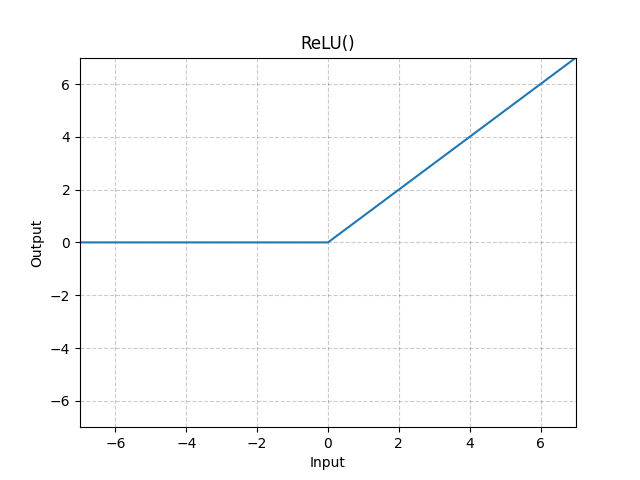
\includegraphics[width=\linewidth]{figures/equations/ReLU.png}
%         \caption{}
%         \label{subfig:funcion-minimo-local}
%     \end{subfigure}\hfill % <-- \hfill
%     \begin{subfigure}{.475\linewidth}
%         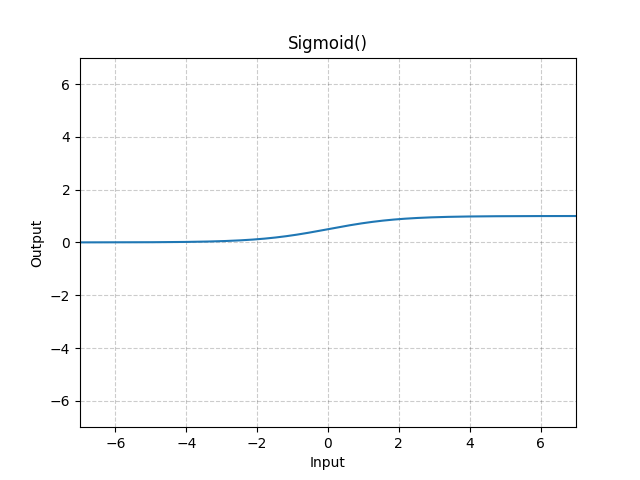
\includegraphics[width=\linewidth]{figures/equations/Sigmoid.png}
%         \caption{}
%         \label{subfig:funcion-punto-de-silla}
%     \end{subfigure}
%     \caption{Mínimos locales y puntos de silla}
%     \label{fig:locales}
% \end{figure}

% endregion El descenso de gradiente

\subsubsection{Optimizadores} \label{optimizers}
% region Optimizadores
% TODO: definición
% TODO: Tipos
% TODO: Usos
Los optimizadores son los algoritmos que buscan encontrar la mejor solución para un problema, esto se utilizan en conjunto con el descenso de gradiente para mejorar su eficiencia y rendimiento, generalmente minimizando o maximizando una función objetiva al ajustar sus parámetros. Existen muchos optimizadores que nos permiten explorar de forma eficiente el espacio de posibles soluciones.

% https://interactivechaos.com/es/manual/tutorial-de-machine-learning/adagrad

Estos son algunos de los optimizadores más famosos.
\begin{enumerate}
    \item \textbf{SGD} (Stochastic Gradient Descent with Momentum): Descenso de gradiente estocástico con momentum.
    \item \textbf{Adam} (Adaptive Moment Estimation): Descenso de gradiente con tasa de aprendizaje adaptativa.
    \item \textbf{Adamax} (Adaptive Moment Estimation with Infinity Norm):  variante de Adam que utiliza la norma infinita en lugar de la norma 2 para calcular y actualizar el término de escala máximo.
    \item \textbf{AdaGrad} (Adaptative Gradient Algorithm): variante de \textit{SGD} en la que se emplean distintas tasas de aprendizaje teniendo en cuenta el gradiente acumulado en cada una de las variables.
    \item \textbf{RMSprop} (Root Mean Square Propagation): variante de \textit{AdaGrad} en la que, en lugar de mantener un acumulado los gradientes, se utiliza el concepto de ``ventana'' para considerar los gradientes más recientes.
\end{enumerate}

% endregion Optimizadore

\subsubsection{Funciones de activación} \label{sec:activations-functions}
% region Funciones de activación
% TODO: definición, explicación y usos
% TODO: tipos, solo mostramos las más importantes
% TODO: 
A la salida de una neurona artificial debe existir un filtro o umbral que modifica el resultado previo, está función puede imponer un umbral que debe pasar para que el valor se transmita a la siguiente capa, esta función se le conoce como función de activación.
Esto introduce no linealidad en el modelo, permitiendo que la red aprenda patrones complejos y mejora su capacidad de representación.

Existen muchas funciones de activación que modifican la red neuronal de distintas formas.
Se suelen clasificar en dos categorías, funciones de activación de suma ponderada, no lineales u otras.

% TODO: extender

\paragraph*{F. Activaciones no lineales - \textit{Non-linear Activations (weighted sum, nonlinearity)} \cite{pytorch2024github}}

% \begin{enumerate}
%     \item \textbf{ReLU}:
%     \item[] \begin{equation} \varphi(x) = \operatorname*{max}(0,x) \end{equation}
%     \item \textbf{LeakyReLU}:
%     \item[] \begin{equation} \varphi(x) = \operatorname*{max}\left(0,x\right) + \operatorname*{negative\_slope} * \operatorname*{min}\left(0,x\right)  \end{equation}

%     \item \textbf{Softplus}:
%     \item[] \begin{equation} \varphi(x) = \frac{1}{\beta} \operatorname*{log}\left(1+e^{\beta x}\right) \end{equation}
%     \item \textbf{SoftSign}:
%     \item[] \begin{equation} \varphi(x) = \frac{x}{1+\lvert x \rvert} \end{equation}

%     \item \textbf{Tanh}:
%     \item[] \begin{equation} \varphi(x) = \frac{e^{x}-e^{-x}}{e^{x}+e^{-x}} \end{equation}
%     \item \textbf{Sigmoid}:
%     \item[] \begin{equation} \varphi(x) = \frac{1}{1+e^{-x}} \label{eq:sigmoid} \end{equation}
% \end{enumerate}

\begin{figure}[H]
    \centering
    \captionsetup{justification=centering}

    % ReLU
    \begin{subfigure}{.475\linewidth}
        \centering
        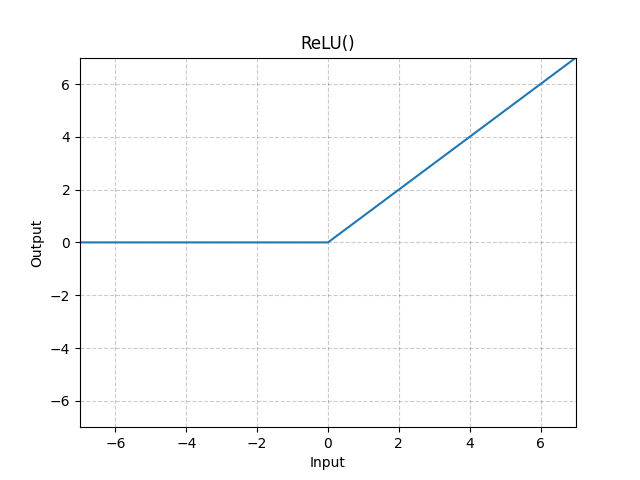
\includegraphics[width=0.75\linewidth]{figures/equations/ReLU.png}
        \caption{Función de activación ReLU.\newline{}Fuente: \href{https://pytorch.org/docs/stable/generated/torch.nn.ReLU.html}{Pytorch torch.nn.ReLU}}
        \label{subfig:torch.nn.ReLU}
    \end{subfigure}\hfill % <-- "\hfill"
    \begin{subfigure}{.475\linewidth}
        \centering
        \begin{equation*}\varphi(x) = \operatorname*{max}(0,x)\end{equation*}
        \caption{Función de activación ReLU.\newline{}Fuente: \href{https://pytorch.org/docs/stable/generated/torch.nn.ReLU.html}{Pytorch torch.nn.ReLU}}
        \label{subfig:eq-torch.nn.ReLU}
    \end{subfigure}

    % LeakyReLU
    \medskip % create some *vertical* separation between the graphs
    \begin{subfigure}{.475\linewidth}
        \centering
        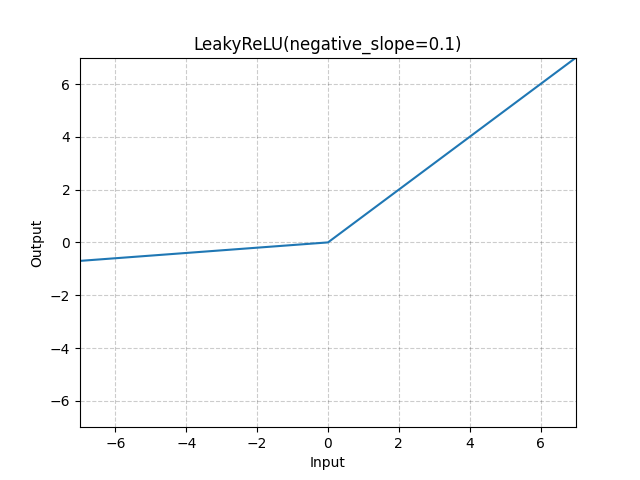
\includegraphics[width=0.75\linewidth]{figures/equations/LeakyReLU.png}
        \caption{Función de activación LeakyReLU.\newline{}Fuente: \href{https://pytorch.org/docs/stable/generated/torch.nn.LeakyReLU.html}{Pytorch torch.nn.LeakyReLU}}
        \label{subfig:torch.nn.LeakyReLU}
    \end{subfigure}\hfill
    \begin{subfigure}{.475\linewidth}
        \centering
        \begin{small}
            \begin{equation*}
                \varphi(x) = \operatorname*{max}\left(0,x\right) + \operatorname*{negative\_slope} * \operatorname*{min}\left(0,x\right)
            \end{equation*}
        \end{small}
        \caption{Función de activación LeakyReLU.\newline{}Fuente: \href{https://pytorch.org/docs/stable/generated/torch.nn.LeakyReLU.html}{Pytorch torch.nn.LeakyReLU}}
        \label{subfig:eq-torch.nn.LeakyReLU}
    \end{subfigure}

    \medskip
    \begin{subfigure}{.475\linewidth}
        \centering
        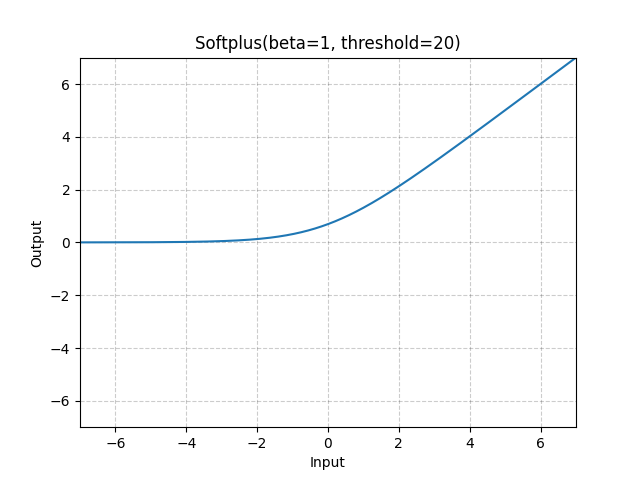
\includegraphics[width=0.75\linewidth]{figures/equations/Softplus.png}
        \caption{Función de activación Softplus.\newline{}Fuente: \href{https://pytorch.org/docs/stable/generated/torch.nn.Softplus.html}{Pytorch torch.nn.Softplus}}
        \label{subfig:torch.nn.Softplus}
    \end{subfigure}\hfill
    \begin{subfigure}{.475\linewidth}
        \centering
        \begin{equation*} \varphi(x) = \frac{1}{\beta} \operatorname*{log}\left(1+e^{\beta x}\right) \end{equation*}
        \caption{Función de activación Softplus.\newline{}Fuente: \href{https://pytorch.org/docs/stable/generated/torch.nn.Softplus.html}{Pytorch torch.nn.Softplus}}
        \label{subfig:eq-torch.nn.Softplus}
    \end{subfigure}

    \caption{Funciones de activación no lineales}
    \label{fig:p1--equations--Non-linear-Activations}
\end{figure}

\begin{figure}[H]
    \centering
    \captionsetup{justification=centering}

    \begin{subfigure}{.475\linewidth}
        \centering
        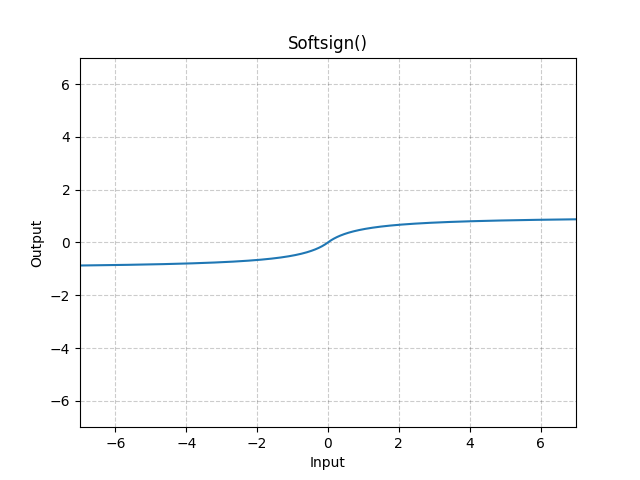
\includegraphics[width=0.75\linewidth]{figures/equations/Softsign.png}
        \caption{Función de activación Softsign.\newline{}Fuente: \href{https://pytorch.org/docs/stable/generated/torch.nn.Softsign.html}{Pytorch torch.nn.Softsign}}
        \label{subfig:torch.nn.Softsign}
    \end{subfigure}
    \begin{subfigure}{.475\linewidth}
        \centering
        \begin{equation*} \varphi(x) = \frac{x}{1+\lvert x \rvert} \end{equation*}
        \caption{Función de activación Softsign.\newline{}Fuente: \href{https://pytorch.org/docs/stable/generated/torch.nn.Softsign.html}{Pytorch torch.nn.Softsign}}
        \label{subfig:eq-torch.nn.Softsign}
    \end{subfigure}

    \medskip
    \begin{subfigure}{.475\linewidth}
        \centering
        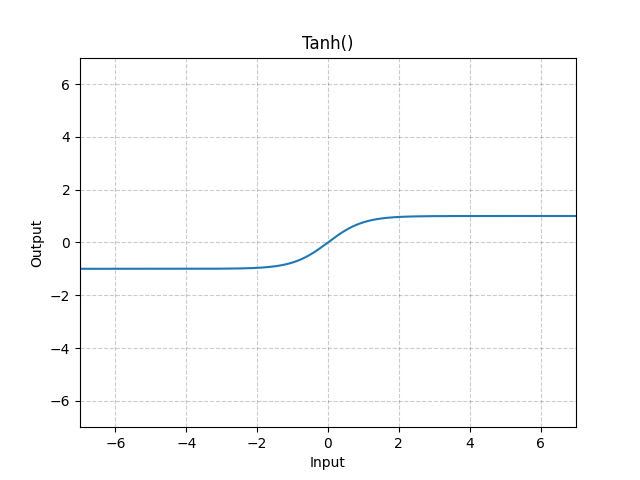
\includegraphics[width=0.75\linewidth]{figures/equations/Tanh.png}
        \caption{Función de activación Tanh.\newline{}Fuente: \href{https://pytorch.org/docs/stable/generated/torch.nn.Tanh.html}{Pytorch torch.nn.Tanh}}
        \label{subfig:torch.nn.Tanh}
    \end{subfigure}\hfill
    \begin{subfigure}{.475\linewidth}
        \centering
        \begin{equation*} \varphi(x) = \frac{e^{x}-e^{-x}}{e^{x}+e^{-x}} \end{equation*}
        \caption{Función de activación Tanh.\newline{}Fuente: \href{https://pytorch.org/docs/stable/generated/torch.nn.Tanh.html}{Pytorch torch.nn.Tanh}}
        \label{subfig:eq-torch.nn.Tanh}
    \end{subfigure}

    \medskip
    \begin{subfigure}{.475\linewidth}
        \centering
        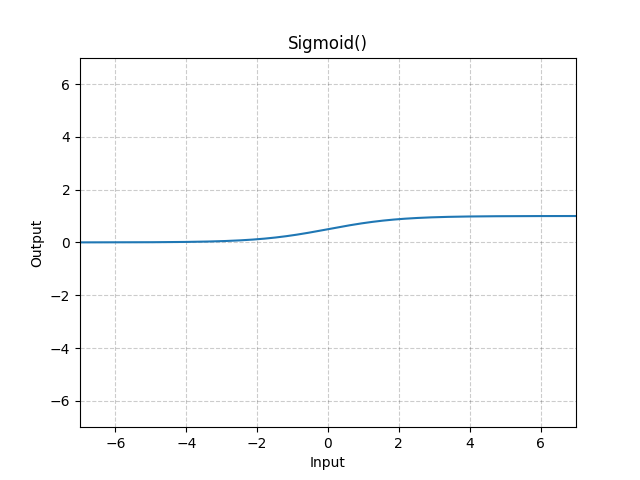
\includegraphics[width=0.75\linewidth]{figures/equations/Sigmoid.png}
        \caption{Función de activación Sigmoid.\newline{}Fuente: \href{https://pytorch.org/docs/stable/generated/torch.nn.Sigmoid.html}{Pytorch torch.nn.Sigmoid}}
        \label{subfig:torch.nn.Sigmoid}
    \end{subfigure}\hfill
    \begin{subfigure}{.475\linewidth}
        \centering
        \begin{equation*} \varphi(x) = \frac{1}{1+e^{-x}} \end{equation*}
        % \label{eq:sigmoid} 
        \caption{Función de activación Sigmoid.\newline{}Fuente: \href{https://pytorch.org/docs/stable/generated/torch.nn.Sigmoid.html}{Pytorch torch.nn.Sigmoid}}
        \label{subfig:eq-torch.nn.Sigmoid}
    \end{subfigure}

    \caption{Funciones de activación no lineales}
    \label{fig:p2--equations--Non-linear-Activations}
\end{figure}


\paragraph*{F. Activaciones no lineales - \textit{Non-linear Activations (other)} \cite{pytorch2024github}}
% TODO: explicar las funciones de activación no lineales más importantes

\begin{enumerate}
    \item \textbf{Softmax}: Aplica la función Softmax a un Tensor de entrada ${n}$-dimensional re-escalándolos para que los elementos del Tensor de salida ${n}$—dimensional se encuentren en el rango [0,1]. \cite{pytorch2024github}
    \item[] \begin{equation} \varphi(x_{i}) = \frac{e^{x_{i}}}{\sum_{j}{e_{j}}} \end{equation}
        % TODO, añadir más si se requiere
\end{enumerate}


% endregion Funciones de activación

\subsubsection{Tipos de capas}
% region Tipos de capas
% TODO: Capas de entrada, ocultas y de salida.
% TODO: Capas densas, no lineales, con y sin pesos
% TODO: Usos, ventajas y desventajas, paralelización

% Non-linear Activations (weighted sum, nonlinearity)
% Non-linear Activations (other)
% - Convolution Layers
% - Pooling layers
% - Padding Layers
% - Normalization Layers
% - Recurrent Layers
% - Linear Layers
% - Dropout Layers
% - Sparse Layers
% * Distance Functions
% * Loss Functions
% Transformer Layers
% Vision Layers
% Shuffle Layers


Existen una gran variedad de capas con distintos propósitos, permiten organizar y estructurar el funcionamiento de la red durante el proceso de aprendizaje. Cada capa influye con un propósito específico, contribuyendo de manera única al funcionamiento global de la red.

Algunas de las características de las capas más famosas son las siguientes.

\begin{itemize}
    \item \textbf{Capas densas y dispersas (Denses and Sparses Layers)}:
    \item[]
        \begin{itemize}
            \item \textbf{Capas densas}: Capas que conectan todas las neuronas de una capa con todas las de la capa siguiente.
            \item[] Son ampliamente utilizadas en \acrshort{ANN} tradicionales  para tareas de clasificación y regresión.
            \item \textbf{Capas dispersas}: Capas que contienen conexiones dispersas entre neuronas, lo que implica que no todas las neuronas están conectadas entre sí.
            \item[] Se utilizan para reducir la complejidad computacional y el consumo de memoria en modelos grandes.
        \end{itemize}
    \item \textbf{Capas lineales (Linear Layers)}:
    \item[]
        \begin{itemize}
            \item Estas capas generalmente se combinan con funciones de activación no lineales para introducir no linealidad en la red neuronal.
            \item Tanto \texttt{nn.Linear} como \texttt{nn.Bilinear} realizan transformaciones lineales de las entradas ponderando los pesos. \texttt{nn.Identity} no realiza ninguna transformación, y \texttt{nn.LazyLinear} puede realizar transformaciones lineales perezosas.
            \item Proporcionan flexibilidad al permitir ajustar sus parámetros según las necesidades del modelo o la tarea.
        \end{itemize}
    \item \textbf{Capas Convolucionales (Convolutional Layers)}:
          % se especializan en detectar la presencia de características proporcionadas por la entrada del modelo.
    \item[]
        \begin{itemize}
            \item Aplican filtros o convoluciones a la entrada para detectar patrones como bordes, texturas y formas.
            \item Se utilizan principalmente para procesar datos de imágenes y extraer características relevantes.
            \item Son la base del funcionamiento en tareas de clasificiación de imágenes o de segmentación de imágenes.
        \end{itemize}
    \item \textbf{Capas de Pooling (Pooling Layers)}:
          % se especializan en comprimir la información de las imágenes preservando la abstracción de las características más importantes, ayudan a reducir el {overfitting}, existen múltiples variantes cómo \texttt{nn.MaxPool1d} o \texttt{nn.AvgPool1d}.
    \item[]
        \begin{itemize}
            \item Comprimen la dimensionalidad de las características extraídas de las capas convolucionales. Se usan entre capas convolucionales.
            \item Existen múltiples variantes cómo \texttt{nn.MaxPool1d} o \texttt{nn.AvgPool1d} que seleccionan los valores más significativos de una región dada.
            \item Ayudan a reducir el {overfitting}, simplificar la representación de características, reducir el coste computacional, etc.
        \end{itemize}
    \item \textbf{Capas de Padding (Paddings Layers)}:
          % se usan para ajustar las dimensiones de los datos de entrada para que sean compatibles con ciertas operaciones, mejoran el rendimiento.
    \item[]
        \begin{itemize}
            \item Se usan para ajustar las dimensiones de los datos de entrada, permiten después aplicar operaciones.
            \item Añade ceros o constantes alrededor de los bordes de regiones para ajustar el tamaño a posteriores operaciones.
            \item Previenen la pérdida de información en los bordes.
        \end{itemize}
    \item \textbf{Capas de Normalización (Normalization Layers)}:
          % se usan para mejorar el rendimiento y la estabilidad del entrenamiento, realizan operaciones sobre los mapas de activación, existen variantes, las más usadas son \texttt{nn.BatchNorm1d} y \texttt{nn.LayerNorm} que permiten aplicar una normalización por lotes o por capas respectivamente.
    \item[]
        \begin{itemize}
            \item Realizan operaciones sobre los mapas de activación, se utilizan para estabilizar y acelerar el entrenamiento de la red.
            \item Algunas de las capas relevantes son \texttt{nn.BatchNorm1d} y \texttt{nn.LayerNorm}, estás permiten aplicar una normalización por lotes o por capas respectivamente.
            \item Ayudan a mantener la distribución de activaciones más consistentes durante el entrenamiento.
        \end{itemize}
    \item \textbf{Capas de Dropout (Dropout Layers)}:
          % se usan para entrenamientos más estables eliminando dependencias, evitan el sobreajuste {overfitting}, esto lo hacen desactivando de forma estocástica ciertas neuronas en las distintas iteraciones.
    \item[]
        \begin{itemize}
            \item Se desactivan aleatoriamente un porcentaje de neuronas en la capa, esto evita dependencias en el entrenamiento, además de generalizar mejor.
            \item Es una técnica de regularización que reduce el sobreajuste, se usan para entrenamientos más estables eliminando dependencias.
        \end{itemize}
    \item \textbf{Capas Recurrentes (Recurrent Layers)}:
          % se usan para procesar datos secuenciales o de series temporales, su característica principal son que tienen memoria, existen distintas variantes en función de cuando tome el contexto, unidireccionales si solo cuenta el contexto previo o bidireccionales si consideran el previo y posterior. Las más usadas son \texttt{nn.RNN}, \texttt{nn.LSTM} y \texttt{nn.GRU}
    \item[]
        \begin{itemize}
            \item Diseñadas para manejar datos secuenciales o de series temporales.
            \item Incorporan conexiones cíclicas que les permiten propagar información de un paso de tiempo a otro, las más usadas son \texttt{nn.RNN}, \texttt{nn.LSTM} y \texttt{nn.GRU}.
            \item Las capas recurrentes tienen memoria y contexto considerando los estados previos, son útiles para traducción de idiomas, procesamiento del lenguaje natural y reconocimiento de voz.
        \end{itemize}
\end{itemize}

% endregion Tipos de capas 

\subsubsection{Topologías de redes neuronales}
% region topologías
% TODO: explicar la existencia de distintas formas de aplicar las capas de neuronas artificiales y sus resultados
La topología o arquitectura de una red neuronal nos referimos a la organización y disposición de las neuronas en la red, formando capas. Estos parámetros fundamentales determinan cómo se estructura la red.
Se suele considerar el número de capas, número de neuronas por capa, tipo de conexiones (unidireccionales o recurrentes).


\begin{figure}[H]
    \centering
    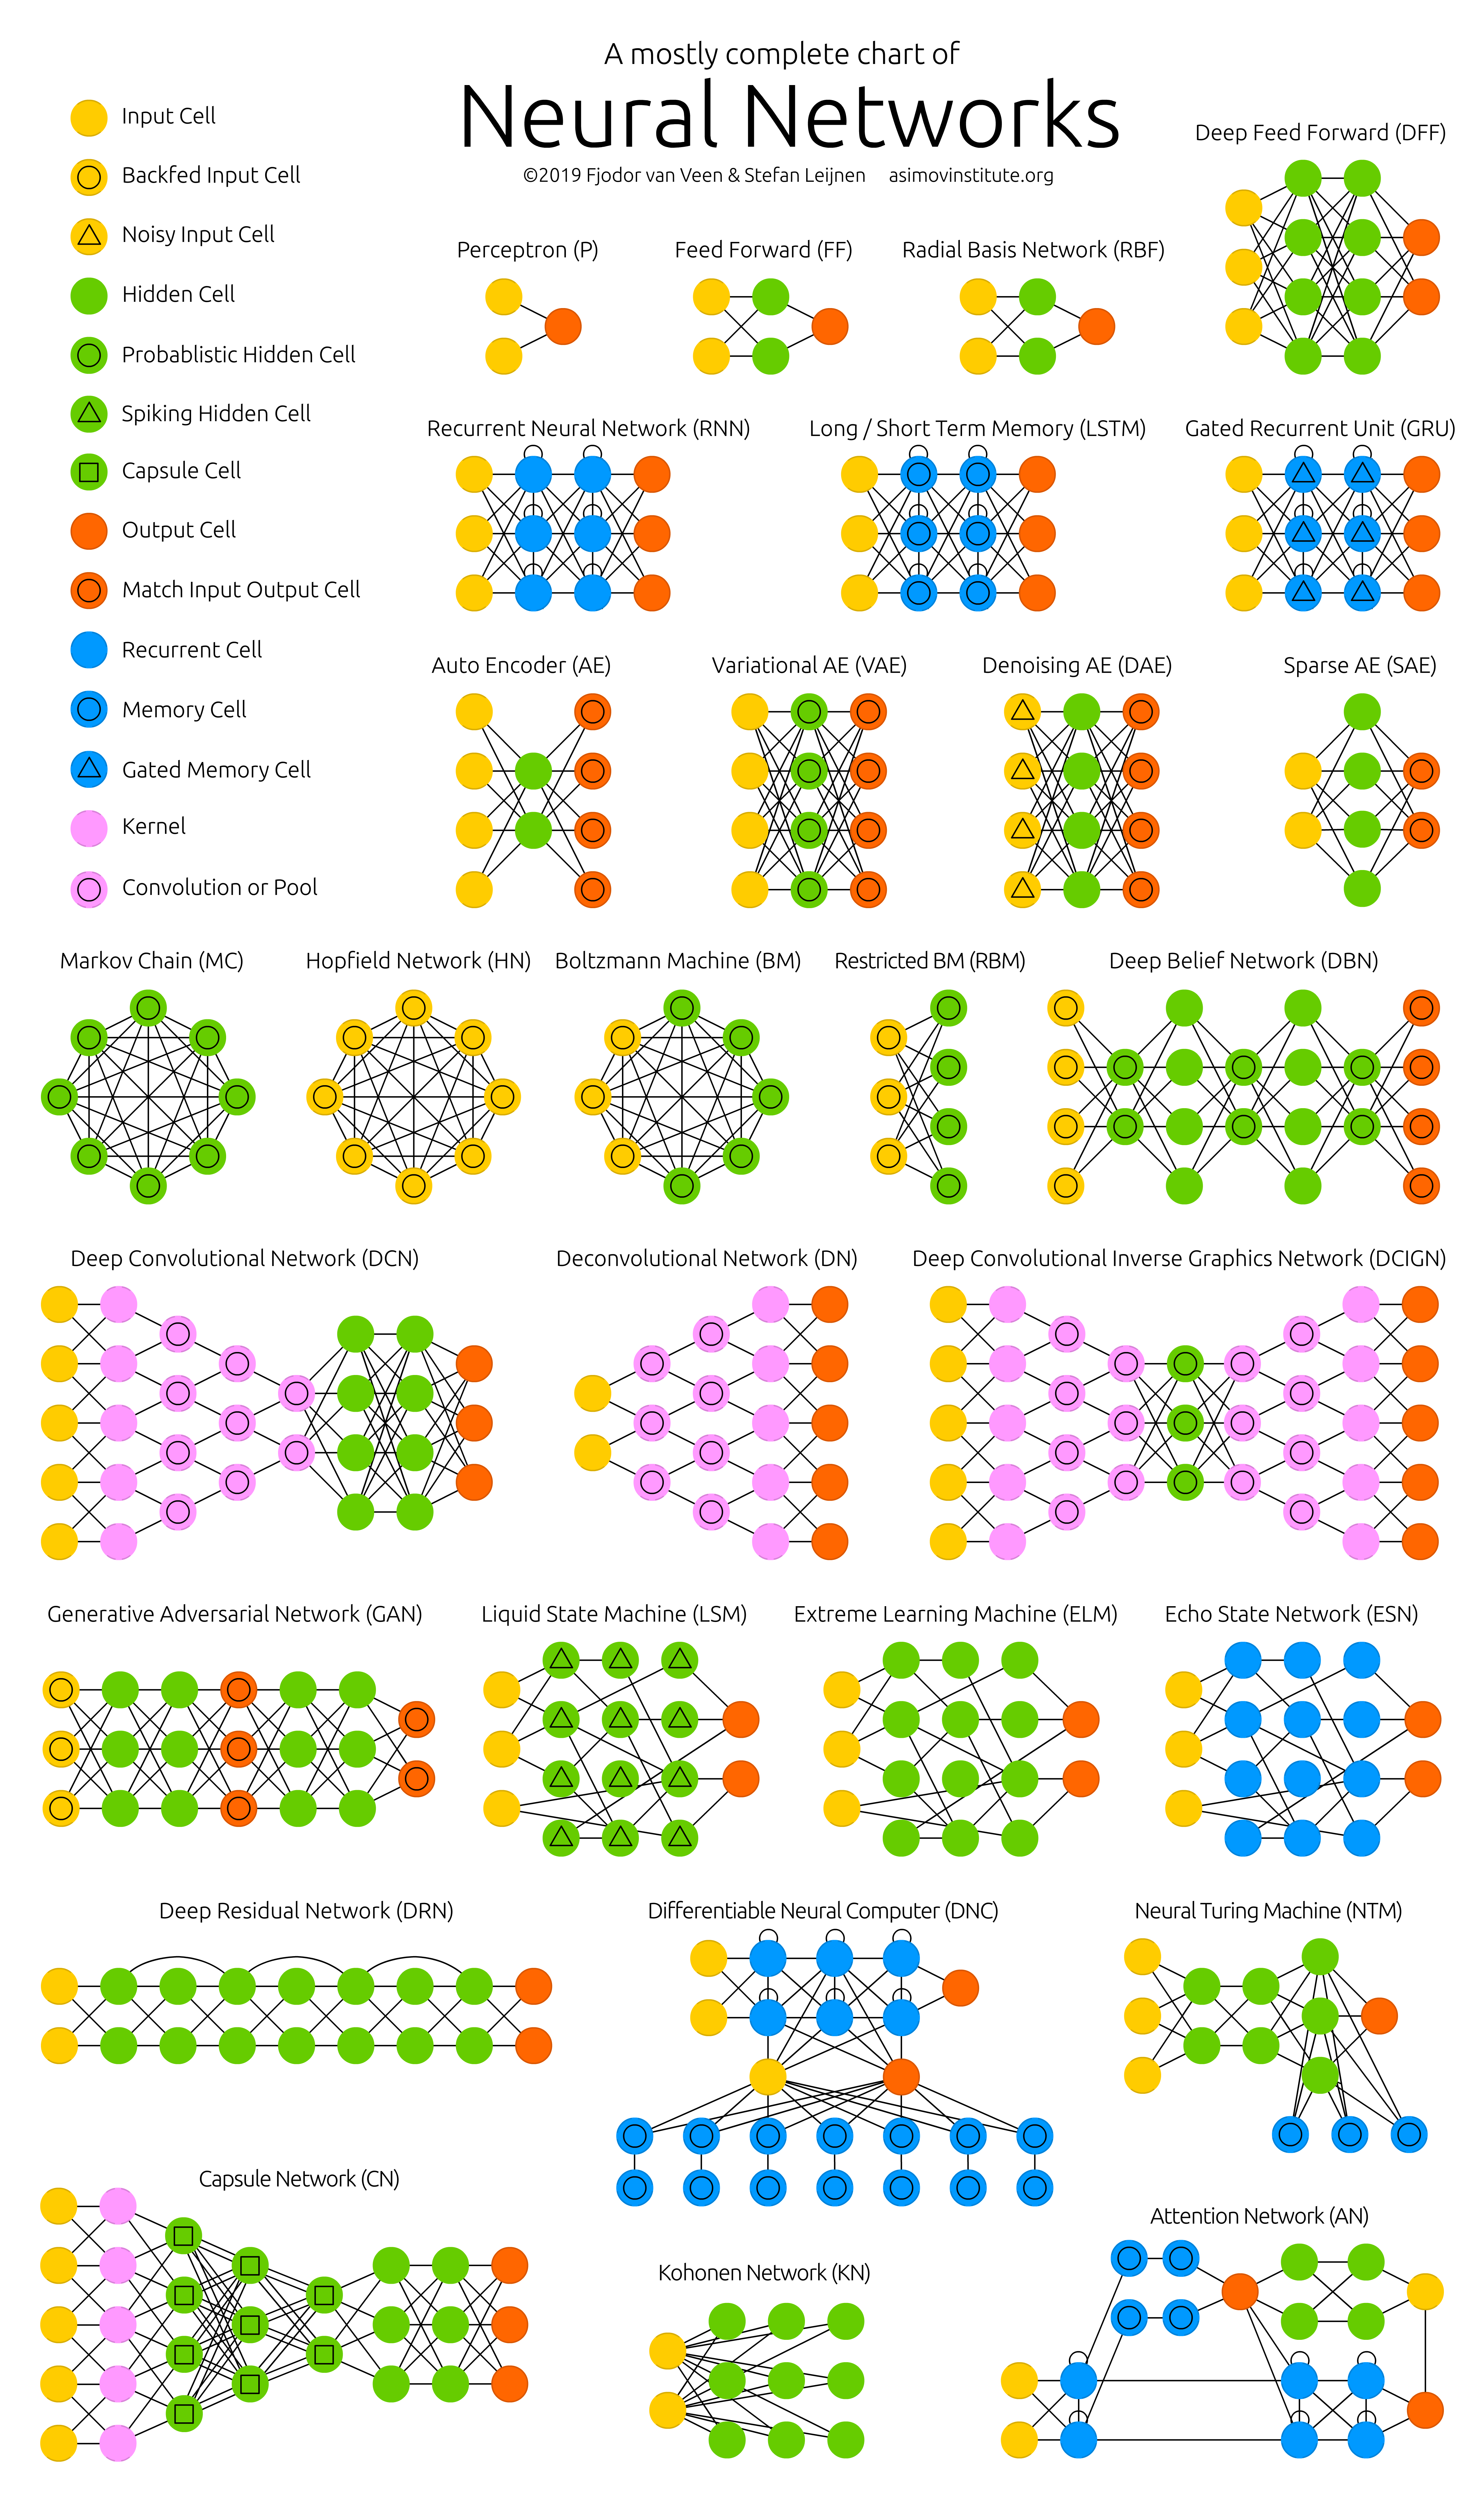
\includegraphics[width=0.65\textwidth]{figures/NeuralNetworkZo19High.png}
    \caption{Topologías de redes neuronales.\newline{}Fuente: \href{https://www.asimovinstitute.org/neural-network-zoo/}{The neural network zoo}}
    \label{fig:NeuralNetworkZo19High}
\end{figure}
% endregion topologías


% endregion subsection Redes neuronales artificiales

\subsection[\texorpdfstring{Autocodificador Variacional \\ \textit{Variational Autoencoders (VAE)}}{Autocodificador Variacional - Variational Autoencoders (VAE)}]{Autocodificador Variacional \\ \textit{Variational Autoencoders (VAE)}}
% \ref{subsection:divergencia-kl}
Los \gls{VAE} son complejos, ya que se basan en el teorema de \nameref{theorem:bayes}, en la divergencia de {Kullback-Leibler}, junto con los \gls{AE} que son un tipo de arquitectura de red neuronal \acrshort{NN} que dan como salida el mismo tipo de dato que el dato de entrada. Estos modelos comprimen en un espacio latente los datos de entrada para después descomprimir la información. 

Los \gls{AE} son sencillos, pero no funcionan bien para la generación de instancias, pues lo que queremos es generar variaciones de la entrada.

\begin{figure}[H]
    \centering
    \includesvg[width=1\linewidth]{figures/chapter02/autoencoder.drawio.svg}
    \caption{Encoder-Decoder. \newline{}Fuente: Elaboración propia.}
    \label{fig:encoder-decoder}
\end{figure}

Los modelos \gls{VAE} dan una reconstrucción del dato de entrada, tienen múltiples funcionalidades, reducción de la dimensionalidad, compresión de datos, permiten eliminar el ruido, detectar anomalías, generar datos, aprendizaje de representación, traducción de imágenes y relleno de imágenes, etc.

Los \gls{VAE} son modelos predictivos que ha demostrado ser exitosos para aprender de forma no supervisada distribuciones complejas de datos e iterar sobre el espacio latente. Permiten generar instancias complejas nuevas como números manuscritos, rostros humanos o segmentar imágenes \cite{kingma2022autoencodingvariationalbayes}.

\begin{figure}[H]
    \centering
    \includesvg[width=1\linewidth]{figures/chapter02/variational-autoencoders.drawio.svg}
    \caption{Variable Auto-encoder. \newline{}Fuente: Elaboración propia, inspirado en el capítulo 2 El auto-encoder variacional \cite{upm71832}}
    \label{fig:variational-auto-decoder}
\end{figure}

Los \gls{AE} presentan problemas, estos los intentan solucionar \gls{VAE}, como vemos en las figuras \ref{fig:encoder-decoder} y \ref{fig:variational-auto-decoder}, los \gls{AE} agrupan la codificación en grupos distintos y los \gls{VAE} son más continuos, los \gls{VAE} se mapean a una distribución, esto es gracias a que en el codificador de los \gls{VAE} se usan dos vectores, un vector es la mediana ${\mu}$ que indica donde debería estar la codificación en el espacio latente y otro vector es la desviación estándar ${\sigma}$ que representa el área alrededor de ese punto. Según como avanza el entrenamiento, el decodificador aprende los puntos y los vectores que los rodean. \cite{alihamzaaliasiaVQVAE}

El entrenamiento y generación de instancias con \gls{VAE} es el siguiente:

\begin{itemize}
    \item Se eligen dos instancias entre las que se quiere generar.
    \item Se introducen las dos instancias en el codificador y se obtiene un vector latente para cada instancia.
    \item Elige varios vectores intermedios que se encuentre entre los vectores latentes de cada instancia.
    \item Se toman los vectores intermedios y se pasan por el decodificador del para generar las instancias intermedias entre las dos instancias iniciales.
\end{itemize}

Los \gls{VAE} presentan distintos problemas, uno de los principales es que solo aprenden una representación latente continua, para ello aparecen los \gls{VQ-VAE} que estos sí pueden aprender representaciones latentes discretas, realizando reconstrucciones más nítidas. Los \textit{auto encoders} cuantizados añaden una lista de vectores gestionada por un índice, mediante la distancia euclidiana se entrena el decodificador.

\begin{figure}[H]
    \centering
    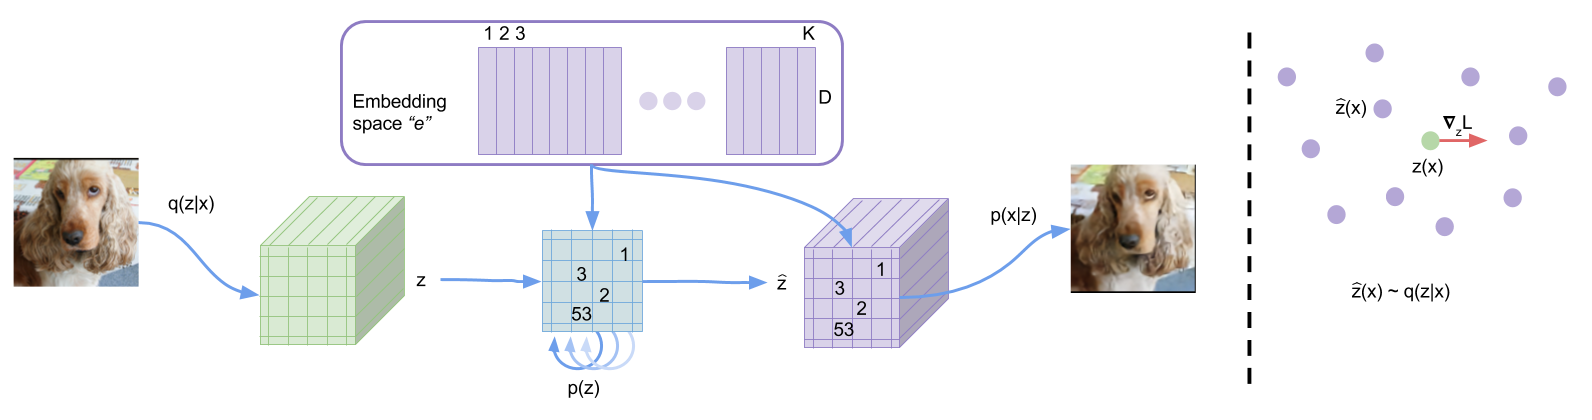
\includegraphics[width=1\linewidth]{figures/chapter02/VQ-VAE.png}
    \caption{Vector Quantised Variational AutoEncoder (VQ-VAE). \newline{}Fuente: Neural Discrete Representation Learning \cite{oord2018neuraldiscreterepresentationlearning}}
    \label{fig:vq-vae}
\end{figure}
\subsection[\texorpdfstring{Redes generativas adversariales \\ \textit{Generative Adversarial Networks (GAN)}}{Redes generativas adversariales - Generative Adversarial Networks (GAN)}]%
{Redes generativas adversariales \\ \textit{Generative Adversarial Networks (GAN)}}
% \subsection{Redes generativas adversariales - \textit{Generative Adversarial Networks (GAN)}}

% region Redes generativas adversariales
% TODO: El concepto de redes antagónicas
% TODO: definición matemática de las dos redes
% TODO: Usos y aplicaciones
% TODO: Ventajas e inconvenientes
% TODO: Arquitecturas derivadas
% README: https://arxiv.org/ftp/arxiv/papers/2302/2302.09346.pdf
Las primeras redes neuronales adversariales se presentaron en la década de los 90 como una curiosidad, no fue hasta 2014 con \textit{Ian Goodfellow} que creo y propuso la primera \gls{GAN}. Su arquitectura estaba formada por dos redes neuronales artificiales, una ``generadora (${G}$)'' y otra ``discriminadora (${D}$)''. La red ${G}$ se encarga de generar instancias del mismo dominio que el conjunto de datos, mientras que la red ${D}$ es la encargada de aceptar o rechazar si los datos generados por la red ${G}$ son reales o falsos. Ambas redes se entrenan conjuntamente de manera que ${G}$ minimiza las detecciones de ${D}$, y a su vez ${D}$ detecte las instancias generadas por ${G}$ \cite{de2023redes}.

Las redes generativas pueden contar con lo que se denomina ruido o \textit{latent space}. El \textit{latent space} es una representación abstracta de las características de los datos de entrada que el generador utiliza para crear nuevos ejemplos que se asemejen con las instancias del conjunto de entrenamiento. El objetivo de nuestras redes generadoras es que aprendan a mapear puntos de este espacio latente a puntos del espacio pertenecientes al conjunto de entrenamiento.

\begin{figure}[H]
    \centering
    \centerline{\includesvg[width=0.99\linewidth]{figures/chapter02/GANs-original.drawio.svg}}
    \caption{Arquitectura de las redes neuronales generativas adversariales.\newline{}Fuente: Elaboración propia.}
    \label{fig:gans-architecture}
\end{figure}

% ;TLTR;
Una \gls{GAN} básica se entrena de forma similar a un algoritmo ``${\min\max}$'', esto está representado en la ecuación \ref{eq:gan-0}. Con este proceso hacemos que la red ${G}$ mejore la generación de instancias haciéndola más parecidas, aunque también puede generar instancias irreales, ya que, aunque las instancias sintéticas superan la validación del discriminador, no son físicamente viables en un contexto real.

% TODO: Explicación espacio latente y código latente

Como podemos observar en la ecuación \ref{eq:gan-0} está compuesta por dos secciones similares que luego se suman, estas partes representan las dos redes neuronales compitiendo y la pérdida (\textit{loss}) de ambas, en función de cómo modifiquemos los distintos componentes y estructuras de las redes neuronales la \gls{GAN} se comportara de una forma u otra, estas modificaciones las veremos en las siguientes secciones.
% https://deepgenerativemodels.github.io/assets/slides/cs236_lecture9.pdf
% https://deepgenerativemodels.github.io/notes/gan/

\begin{equation}
    \min_{G}\max_{D} = \mathbb{E}_{x\sim{}P_{\text{data}}(x)} \left[\log\left(D(x\mid{}y)\right)\right] + \mathbb{E}_{z\sim{}P_{\text{noise}}(z)} \left[\log\left(1-D(G(z\mid{}y))\right)\right]
    \label{eq:gan-0}
\end{equation}

Esto está representado en la Figura \ref{fig:gans-architecture}, donde podemos observar las distintas partes de una red \gls{GAN}. Además, podemos observar la distribución de probabilidad aleatoria representada como ${P_{z}, P_{\text{noise}}}$. El objetivo de la red es la optimización de la distribución de probabilidad de la red generativa ${P_{x}, P_{\text{data}}}$ sea similar a ${G(z)}$, es decir, ${G(z)\sim{}P_{g}}$.

\begin{equation}
    \min_{G}\max_{D} = \mathbb{E}_{x\sim{}P_{\text{data}}} \left[\log\left(D(x)\right)\right] + \mathbb{E}_{z\sim{}P_{\text{noise}}(z)} \left[\log\left(1-D(G(z))\right)\right]
    \label{eq:gan-1}
\end{equation}

La función objetiva está definida por la ecuación \ref{eq:gan-2}, nos referimos con ${\theta}$ a los parámetros de la red ${G}$ y con ${\omega}$ a los parámetros de la red ${D}$. La esperanza de ${f(x)}$ con respecto a la distribución de probabilidad de ${x}$ según ${Q}$ es lo que se denota como ${\mathbb{E}_{x \sim Q}}$.

\begin{equation}
    \min_{\theta}\max_{\omega} = \mathbb{E}_{x\sim{}Q} \left[\log\left(D_{\omega}(x)\right)\right] + \mathbb{E}_{z \sim{}P_{\theta}} \left[\log\left(1-D(G_{\theta}(z))\right)\right]
    \label{eq:gan-2}
\end{equation}

Para que la red ${D}$ funcione deberá recibir tantos datos originales ${x_{real}}$ como datos generados por ${G}$, ${x_{fake}}$, ${G}$ se optimiza al mismo tiempo para que ${D}$ no pueda detectar los datos generados por ${G}$, este proceso está representado en las ecuaciones \ref{eq:gan-3-discriminator-loss} y \ref{eq:gan-4-generator-loss}.

% TODO: revisar este texto
Las redes \gls{GAN} originales produce una probabilidad de que la imagen de entrada proceda de la distribución generadora de datos. Usaban una red \textit{feed-fordward} con función final sigmoidea.

En la ecuación \ref{eq:gan-3-discriminator-loss} podemos observar la función de pérdida de la red discriminadora ${(D)}$, la sección ${\log\left(D(x)\right)}$ es la encargada de dar la probabilidad de que está clasificando correctamente la instancia generada por la red ${G}$, maximizando la sección ${\log\left(1 - D(G(z))\right)}$ conseguimos etiquetar correctamente la instancia falsa generada por la red ${G}$.

\begin{equation}
    \nabla_{\omega_{D}} \frac{1}{m} \sum_{i=1}^{m} \left[ \log\left(D(x^{(i)})\right) + \log\left(1-D(G(z^{(i)}))\right) \right]
    \label{eq:gan-3-discriminator-loss}
\end{equation}

En la ecuación \ref{eq:gan-4-generator-loss} podemos observar la función de pérdida de la red generadora ${(G)}$, la pérdida del generador se calcula a partir de la clasificación (Real, Falsa) del discriminador. Se recompensa si consigue engañar al discriminador y se le penaliza en caso contrario.

\begin{equation}
    \nabla_{\theta_{G}} \frac{1}{m} \sum_{i=1}^{m} \log\left(1-D(G(z^{(i)}))\right)
    \label{eq:gan-4-generator-loss}
\end{equation}
% TODO: EXPLICAR Non-Saturating GAN Loss

\subsubsection{Usos y aplicaciones}

Las redes \gls{GAN} se han usado principalmente para la generación de imágenes, aunque puede generar instancias sintéticas de muchos dominios.

% https://paperswithcode.com/method/vae
% https://paperswithcode.com/method/gan
% https://paperswithcode.com/methods/category/convolutions
% https://towardsdatascience.com/paper-explained-high-resolution-image-synthesis-with-latent-diffusion-models-f372f7636d42

% TODO:
% Clasificación de \gls{GAN}
% https://sh-tsang.medium.com/review-lsgan-least-squares-generative-adversarial-networks-gan-bec12167e915
Algunas de las tareas que se pueden realizar con una red \gls{GAN}

\begin{itemize}
    \item \textbf{Síntesis de imágenes:} permite crear una imagen a partir de unos datos de entrada.
    \item \textbf{Imagen a imagen:} permite ``traducir'' una imagen, es decir, transformar una imagen de un estilo a otro.
    \item \textbf{Escalado de imágenes:} aumentar la resolución de una imagen sin perder calidad, generando datos faltantes para no perder detalles.
    \item \textbf{Eliminación de ruido}: limpiar imágenes de baja calidad, son capaces de mejor la claridad y reconstruir artefactos
    \item \textbf{Detección de manipulación de la cámara:} 
    \item \textbf{Codificación de vídeo:} mejorar la eficiencia de compresión de video mediante la generación de cuadros intermedios o reducción de ruido.
\end{itemize}

% \paragraph{Ventajas e inconvenientes}

\subsubsection{Taxonomía de GANs}
% TODO: Referencias para cada uno

% SURVEY:
% https://dl.acm.org/doi/pdf/10.1145/3459992
% https://arxiv.org/ftp/arxiv/papers/2302/2302.09346.pdf
% https://arxiv.org/pdf/2203.11242.pdf                      GANSurvey
% https://www.researchgate.net/publication/349189619_Generative_Adversarial_Networks_in_Computer_Vision_A_Survey_and_Taxonomy

\begin{figure}[H]
    \centering
    \centerline{\includesvg[width=0.99\linewidth]{figures/chapter02/GANs-Taxonomy.drawio.svg}}
    \caption{Taxonomía de GANs.\newline{}Fuente: Elaboración propia, adaptado del artículo ``GANs Survey'' \cite{GANSurvey_2021ZHENGWEIWANG}}
    \label{fig:gan-taxonomy}
\end{figure}


% =============================================================================================================================
\subparagraph{Conditional Generative Adversarial Network (cGAN) [2014]}
% https://towardsdatascience.com/cgan-conditional-generative-adversarial-network-how-to-gain-control-over-gan-outputs-b30620bd0cc8
% https://archive.is/XTMWw
% https://es.mathworks.com/help/deeplearning/ug/train-conditional-generative-adversarial-network.html
% https://github.com/SolClover/Art054_NN_cGAN
% https://arxiv.org/abs/1411.1784       Conditional Generative Adversarial Nets
% https://arxiv.org/abs/2103.14884      Continuous Conditional (cGAN) with Generator Regularization

% https://arxiv.org/abs/2206.13676
% https://arxiv.org/abs/1611.07004
% de la anterior ( sacaron esta: https://arxiv.org/abs/2103.14884

% Pix2Pix
Las redes \gls{cGAN} \cite{cGAN-mirza2014conditional,cGAN-zheng2021continuous,cGAN-li2022ttscgan,cGAN} o GAN condicional fue una de las primeras derivaciones que se crearon, modifica la arquitectura alterando el ruido introducido, permitiendo condicionar la red con información adicional como etiquetas de clase. Esto permite que la red aprenda a generar instancias de una clase dada.

En esta arquitectura se modifica tanto la red generadora ${G}$ como la red discriminadora ${D}$, de forma que ambas deben conocer la clase de la instancia.
% TODO: Hacer gráfico https://datascientest.com/en/wp-content/uploads/sites/9/2023/09/cgan-1.webp
% Hacer gráfico y añadir referencia a pytorch-gan

\begin{equation}
    \min_{G}\max_{D}
    = \mathbb{E}_{x\sim{}P_{\text{data}}(x)}   \left[ \log{\left( D(x\mid{}y)     \right)} \right]
    + \mathbb{E}_{z\sim{}P_{\text{noise}}(z)}  \left[ \log{\left( D(G(z\mid{}y))  \right)} \right]
\end{equation}

\begin{figure}[H]
    \centering
    \centerline{\includesvg[width=0.99\linewidth]{figures/chapter02/GANs-cGAN.drawio.svg}}
    \caption{Arquitectura Conditional GAN (\gls{cGAN})\newline{}Fuente: Elaboración propia.}
    \label{fig:cGAN}
\end{figure}

% =============================================================================================================================
\subparagraph{Deep Convolutional Generative Adversarial Network (DCGAN) [2015]}
% https://paperswithcode.com/method/dcgan
% https://www.tensorflow.org/tutorials/generative/dcgan?hl=es-419
% https://towardsdatascience.com/deep-convolutional-gan-how-to-use-a-dcgan-to-generate-images-in-python-b08afd4d124e
% https://github.com/sthalles/blog-resources/blob/master/dcgan/DCGAN.ipynb
% https://archive.is/MgQCM
% FGSM  -->  https://digibug.ugr.es/handle/10481/72468
Las redes \gls{DCGAN} \cite{DCGAN-radford2016unsupervised,DCGAN-viola2020faultface,DCGAN-aslan2019deep,DCGAN-curto2020highresolution} son una de las redes generativas más famosas y usadas dentro de su ámbito por las ventajas de rendimiento, además estas redes generan detalles de alta resolución partiendo de puntos espacialmente locales de un mapa de características reducido.
% Las GAN convolucionales tradicionales generan detalles de alta resolución en función únicamente de puntos espacialmente locales en mapas de características de menor resolución. 

El discriminador es un clasificador de imágenes basado en \gls{CNN}, frente al generador que a partir de una semilla (ruido) generara imágenes apilando distintas capas.

Las \gls{DCGAN} alteran las capas en ${D}$ cambiando cualquier capa de agrupación (\textit{pooling layers}) por convoluciones escalonadas y en la red ${G}$ las agrupaciones por convoluciones escalonadas fraccionadas, usan \texttt{Batchnorm} en ambas  redes, eliminan capas ocultas de tipo \textit{fully-connected}, usan funciones de activación \texttt{ReLU} en el  generador para todas las capas excepto en la capa de salida que usan \texttt{Tanh} \cite{ibm-gradient-descent}.
% TODO svg

% TODO: ACGAN
% \subparagraph{Auxiliary Classifier Generative Adversarial Network (ACGAN)}






% =============================================================================================================================
\subparagraph{Semi-supervised Generative Adversarial Network (SGAN) [2016]}
% https://towardsdatascience.com/supervised-learning-but-a-lot-better-semi-supervised-learning-a42dff534781
% https://towardsdatascience.com/semi-supervised-learning-with-gans-9f3cb128c5e
% https://archive.is/HCS4V
% https://arxiv.org/abs/1606.01583
En las redes \gls{SGAN} \cite{SGAN-odena2016semisupervised}, la red generadora ${G}$ como la red discriminadora ${D}$ cuentan con datos semi-supervisados, esto difiere de una \gls{GAN} al modificar la red discriminadora con un clasificador. Aprende a clasificar las muestras en diferentes clases en función de las etiquetas dadas.

El uso de estos datos semi-supervisados y de un clasificador en la red discriminadora ${D}$, mejoran los resultados de ambas redes. Además, permite contar con un volumen mayor de datos.

Se ha demostrado que las redes \gls{SGAN} mejoran el rendimiento de la clasificación en conjuntos de datos restringidos.

En la Figura \ref{fig:SGAN} podemos observar la arquitectura de la red usando datos etiquetados, además del clasificador final de la red ${D}$.

\begin{figure}[H]
    \centering
    \centerline{\includesvg[width=0.99\linewidth]{figures/chapter02/GANs-SGAN.drawio.svg}}
    \caption{Arquitectura Semi-supervised GAN ({SGAN})\newline{}Fuente: Elaboración propia.}
    \label{fig:SGAN}
\end{figure}


% \subparagraph{Conditional Generative Adversarial Network (U-Net-GAN)}
% https://arxiv.org/abs/2002.12655
% https://paperswithcode.com/method/u-net-gan
% https://github.com/boschresearch/unetgan
% https://serp.ai/u-net-generative-adversarial-network/

% =============================================================================================================================
\subparagraph{Couple Generative Adversarial Network (CoGAN) [2016]}
% https://medium.com/codex/review-cogan-coupled-generative-adversarial-networks-gan-273f70b340af
% https://github.com/eriklindernoren/PyTorch-GAN/blob/master/implementations/cogan/cogan.py

Las redes \gls{CoGAN} \cite{CoGAN-liu2016coupled} son dos \gls{GAN} que comparten ciertos pesos de las capas, esto permite distribuir de forma conjunta instancias de varios dominios sin necesidad de incluir tuplas.


\begin{equation}
    \begin{split}
        \min_{G_{1},G_{2}}\max_{D_{1},D_{2}}
        & = \mathbb{E}_{x_{1}\sim{}P_{x_{1}}}  \left[ \log{\left( D_{1}(x_{1}) \right)} \right] + \mathbb{E}_{z\sim{}P_{\text{noise}}(z)}      \left[ \log{\left( D_{1}(G_{1}(z))  \right)} \right]   \\
        & + \mathbb{E}_{x_{2}\sim{}P_{x_{2}}}  \left[ \log{\left( D_{2}(x_{2}) \right)} \right] + \mathbb{E}_{z\sim{}P_{\text{noise}}(z)}      \left[ \log{\left( D_{2}(G_{2}(z))  \right)} \right]
    \end{split}
\end{equation}

En la Figura \ref{fig:CoGAN} podemos observar el funcionamiento básico en una iteración de esta arquitectura, lo más relevante es el trabajo  conjunto de ambas redes por sus pesos compartidos, permitiendo que sea un entrenamiento mucho más rápido.

\begin{figure}[H]
    \centering
    \centerline{\includesvg[width=0.99\linewidth]{figures/chapter02/GANs-CoGAN.drawio.svg}}
    \caption{Arquitectura Couple GAN (CoGAN)\newline{}Fuente: Elaboración propia.}
    \label{fig:CoGAN}
\end{figure}


% =============================================================================================================================
% TODO: ContextEncoder

% =============================================================================================================================
\subparagraph{Patch Generative Adversarial Network (PatchGAN) [2016]}

\gls{PatchGAN} \cite{PatchGAN-isola2018imagetoimage} es una arquitectura en la red discriminadora ${D}$, se emplea en tareas de traducción de imagen por ejemplo en redes \gls{Pix2Pix}, la idea principal es simple, segmentar la imagen en parches (${N \times N}$) y discriminar (real o falso) cada uno de esos parches por separado, se centra en analizar las estadísticas de estilo locales y la estructura de alta frecuencia. Estos discriminadores han demostrado que son eficaces a la hora de generar resultados nítidos y de reducir artefactos. Estos discriminadores se suelen usar en conjunto con redes generadoras ${G}$ \gls{U-Net} \cite{U-Net-ronneberger2015unet} para tareas de traducción de imágenes.

A continuación se explica de forma simplificada las ecuaciones de una red \acrshort{PatchGAN}, debemos recordar que estas redes son \acrshort{ConvNET} \href{https://github.com/junyanz/pytorch-CycleGAN-and-pix2pix/issues/39}{PatchGAN Discriminator}

Se ha demostrado que \gls{PatchGAN} reduce los artefactos \cite{PatchGAN-isola2018imagetoimage}, además de que se puede usar en multitud de otras redes como un complemento que mejora la velocidad de entrenamiento y resultados. En el estudio

% Distancia L1
\begin{equation}
    \mathcal{L}_{L1}(G) = \mathbb{E}_{x,y,z} \left[ {\lVert y - G(x,z) \rVert}_{1} \right]
    \label{eq:L1}
\end{equation}

% =============================================================================================================================
\subparagraph{Cycle Generative Adversarial Network (CycleGAN) [2017]}
% https://paperswithcode.com/method/cyclegan
% https://arxiv.org/abs/1703.10593v7
% https://www.tensorflow.org/tutorials/generative/cyclegan?hl=es-419
% https://junyanz.github.io/CycleGAN/
% https://hardikbansal.github.io/CycleGANBlog/
% https://medium.com/analytics-vidhya/the-beauty-of-cyclegan-c51c153493b8
Las redes \gls{CycleGAN} \cite{CycleGAN-zhu2020unpaired,CycleGAN-caleb2021Unpaired,CycleGAN-theiler2019thebeautyofcyclegan} se componen por dos generadores y dos discriminadores, esta red es similar a las redes \gls{Pix2Pix} \cite{pix2pix-isola2018imagetoimage}, ya que lo que hacen es ``traducir'' una instancia a otro dominio, estas redes que a su vez deriva de las redes \gls{cGAN}.

El funcionamiento de estas redes es el siguiente, el primer generador ${\GenXtoY}$, toma la imagen ${x}$ del dominio ${X}$ y la asigna a ${\hat{y}}$, se comprueba con el discriminador ${D_{Y}}$ que ${\hat{y}}$ sea similar a las instancias reales pertenecientes al dominio ${Y}$, este discriminador clasificará si la instancia es una muestra real perteneciente al dominio ${Y}$ o es una instancia generada por ${\GenXtoY}$.

% TODO: terminar explicación de cyclegan

Estas redes permiten extraer las características de un dominio e incorporar esas características a otro dominio con las ventajas de que no necesita de datos de entrenamiento emparejados.

\begin{figure}[H]
    \centering
    \begin{tikzpicture}[node distance=3cm]
        \node (tagX) [draw, minimum size=1.25cm] at (0,0) {$X$};
        \node (tagY) [draw, minimum size=1.25cm, right=of tagX] {$Y$};
        \draw[->, bend left=35] (tagX) to node[above] {${\GenXtoY(x) = \hat{y}}$} (tagY);
        \draw[->, bend left=35] (tagY) to node[below] {${\GenYtoX(y) = \hat{x}}$} (tagX);
        \draw[->, dashed] (tagX.north) -- ++(0,1.25) node[pos=1, right] {$D_{X}$};
        \draw[->, dashed] (tagY.north) -- ++(0,1.25) node[pos=1, right] {$D_{Y}$};
    \end{tikzpicture}
    \caption{Representación CycleGAN}
    \label{fig:fig-cyclegan}
\end{figure}

Función de mapeo para el paso de ${\GenXtoY}$ y el discriminador $D_{Y}$ \ref{eq:cycle-gan-x-to-y}

\begin{equation}
    \begin{split}
        \mathcal{L}_{GAN} (\GenXtoY, D_{Y}, X, Y)
        & = \mathbb{E}_{x\sim{}P_{\text{data}}(x)} \left[\log{\left(1 - D_{Y}(\GenXtoY(x))\right)}\right]     \\
        & + \mathbb{E}_{y\sim{}P_{\text{data}}(y)} \left[\log{\left(D_{Y}(y)\right)}\right]                   \\
    \end{split}
    \label{eq:cycle-gan-x-to-y}
\end{equation}

Función de mapeo para el paso de ${\GenYtoX}$ y el discriminador $D_{X}$ \ref{eq:cycle-gan-y-to-x}

\begin{equation}
    \begin{split}
        \mathcal{L}_{GAN} (\GenYtoX, D_{X}, Y, X)
        & = \mathbb{E}_{x\sim{}P_{\text{data}}(x)} \left[\log{\left(1 - D_{X}(\GenYtoX(x))\right)}    \right]     \\
        & + \mathbb{E}_{y\sim{}P_{\text{data}}(y)} \left[\log{\left(    D_{X}(y)          \right)}    \right]     \\
    \end{split}
    \label{eq:cycle-gan-y-to-x}
\end{equation}

Cada uno de estos generadores ${\GenXtoY}$ y ${\GenYtoX}$ transforman los datos de un dominio a otro, pasando por las siguientes tres fases, \textbf{codificación} usando capas convolucionales, \textbf{transformación} usando bloques \textit{ResNet} y por último la \textbf{descodificación} usando capas convolucionales inversas y una última capa convolucional \cite{CycleGAN-blog}.

A estas dos métricas se le añade la pérdida del ciclo \ref{eq:cycle-gan-l-cyc} esta fórmula se refiere a la consistencia de las transformaciones, si tomamos una instancia del dominio ${X}$ y la pasamos al dominio ${Y}$, si volvemos a pasarla al dominio ${X}$ debe ser consistente.

\begin{equation}
    \begin{split}
        \mathcal{L}_{cyc} (\GenXtoY,\GenYtoX)
        & = \mathbb{E}_{x\sim{}P_{\text{data}}(x)} \left[{\mathrm{MAE}\left(\GenYtoX(\GenXtoY(x)) - x\right)}\right] \\
        & + \mathbb{E}_{y\sim{}P_{\text{data}}(y)} \left[{\mathrm{MAE}\left(\GenXtoY(\GenYtoX(y)) - y\right)}\right] \\
    \end{split}
    \label{eq:cycle-gan-l-cyc}
\end{equation}

En este punto tenemos tres perdidas, a la que podemos añadir la pérdida de la identidad \ref{eq:cycle-gan-l-identity} para mejorar el resultado, esto significa que el generador para datos de un dominio debe dar resultados similares a su dominio, es decir ${\GenXtoY(x) \approx \hat{x}}$ y ${\GenYtoX(y) \approx \hat{y}}$, añadir está pérdida ayuda a preservar las características generales del dominio de origen (colores y tinte en caso imágenes).

\begin{equation}
    \begin{split}
        \mathcal{L}_{identity} (\GenXtoY,\GenYtoX)
        & = \mathbb{E}_{x\sim{}P_{\text{data}}(x)} \left[{\mathrm{MAE}\left(\GenXtoY(x) - x\right)}\right] \\
        & + \mathbb{E}_{y\sim{}P_{\text{data}}(y)} \left[{\mathrm{MAE}\left(\GenYtoX(y) - y\right)}\right] \\
    \end{split}
    \label{eq:cycle-gan-l-identity}
\end{equation}

\begin{itemize}
    \item La pérdida adversarial de ${\GenXtoY}$ contra ${D_{Y}}$.
    \item La pérdida adversarial de ${\GenYtoX}$ contra ${D_{X}}$.
    \item La pérdida del ciclo para el generador ${\GenXtoY}$ y ${\GenYtoX}$.
    \item La pérdida de identidad ${\GenXtoY(x) \approx \hat{x}}$ y ${\GenYtoX(y) \approx \hat{y}}$
\end{itemize}

\begin{equation}
    \begin{split}
        \mathcal{L} (\GenXtoY, \GenYtoX, D_{X}, D_{Y})
        & =            \mathcal{L}_{GAN}       \left(\GenXtoY, D_{Y}, X, Y \right) \\
        & +            \mathcal{L}_{GAN}       \left(\GenYtoX, D_{X}, Y, X \right) \\
        & + \lambda    \mathcal{L}_{cycle}     \left(\GenXtoY,\GenYtoX     \right) \\
        & + 0.5\lambda \mathcal{L}_{identity}  \left(\GenXtoY,\GenYtoX     \right)
    \end{split}
    \label{eq:cycle-gan-all}
\end{equation}

Esta ecuación \ref{eq:cycle-gan-all} es una generalización de cómo funcionan las \gls{CycleGAN}, en cada caso se deberá implementar de forma distinta. En la figura \ref{fig:CycleGAN-2} podemos observar estos dos generadores y los dos discriminadores funcionando para cada uno de los ciclos de entrenamiento.

% \begin{figure}[H]
%     \centering
%     \centerline{\includesvg[width=1\linewidth]{figures/chapter02/GANs-CycleGAN.drawio.svg}}
%     \caption{Arquitectura Cycle GAN (CycleGAN)\newline{}Fuente: Elaboración propia.}
%     \label{fig:CycleGAN}
% \end{figure}

\begin{figure}[H]
    \centering
    \centerline{\includesvg[width=0.99\linewidth]{figures/chapter02/GANs-CycleGAN-2.drawio.svg}}
    \caption{Arquitectura Cycle GAN (CycleGAN)\newline{}Fuente: Elaboración propia.}
    \label{fig:CycleGAN-2}
\end{figure}




% =============================================================================================================================
\subparagraph{Least Square Generative Adversarial Network (LSGAN) [2016]}
% https://paperswithcode.com/method/lsgan
% https://arxiv.org/abs/1611.04076
% https://sh-tsang.medium.com/review-lsgan-least-squares-generative-adversarial-networks-gan-bec12167e915
Las redes \gls{LSGAN} \cite{LSGAN-mao2017squares} o redes generativas de mínimos cuadrados, en estas arquitecturas se modifica la función de pérdida del discriminador, esto mejora la calidad de las instancias generadas así como el proceso de aprendizaje.
% TODO

A continuación en la ecuación \ref{eq:lsgan} se muestra las funciones objetivo para \gls{LSGAN}, debemos tener en cuenta que ${a}$ son los etiquetas para datos falsos, ${b}$ son datos reales y ${c}$ indica el valor que la red ${G}$ envía a la red ${D}$ para que los valide como verdaderos.

\begin{equation}
    \begin{split}
        \min_{D} &= \frac{1}{2} \mathbb{E}_{x\sim{}P_{\text{data}}(x)}  \left[ (D(x) - b)^{2} \right] + \frac{1}{2} \mathbb{E}_{z\sim{}P_{\text{noise}}(z)} \left[ (D(G(z)) - a)^{2} \right]    \\
        \min_{G} &= \frac{1}{2} \mathbb{E}_{z\sim{}P_{\text{noise}}(z)} \left[ (D(G(z)) - c)^{2} \right]                                                                                        \\
    \end{split}
    \label{eq:lsgan}
\end{equation}

En la Figura \ref{subfig:LSGAN-2} podemos observar el límite de decisión de una \gls{GAN} clásica, frente a la Figura \ref{subfig:LSGAN-3} que representa el límite de decisión de una \gls{LSGAN}


\begin{figure}[H]
    \centering
    \captionsetup{justification=centering}
    % 0.99
    \begin{subfigure}{.30\linewidth}
        \centering
        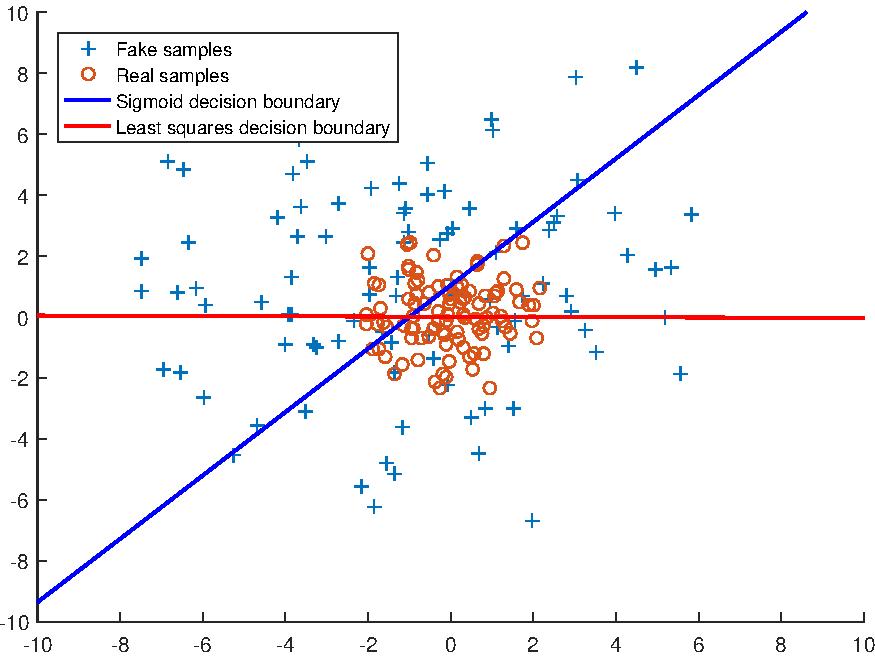
\includegraphics[width=0.95\linewidth]{figures/chapter02/boundary_1.pdf}
        \caption{Límites de decisión de dos funciones de pérdida. }
        \label{subfig:LSGAN-1}
    \end{subfigure}
    \vspace{0.03\linewidth}
    \begin{subfigure}{.30\linewidth}
        \centering
        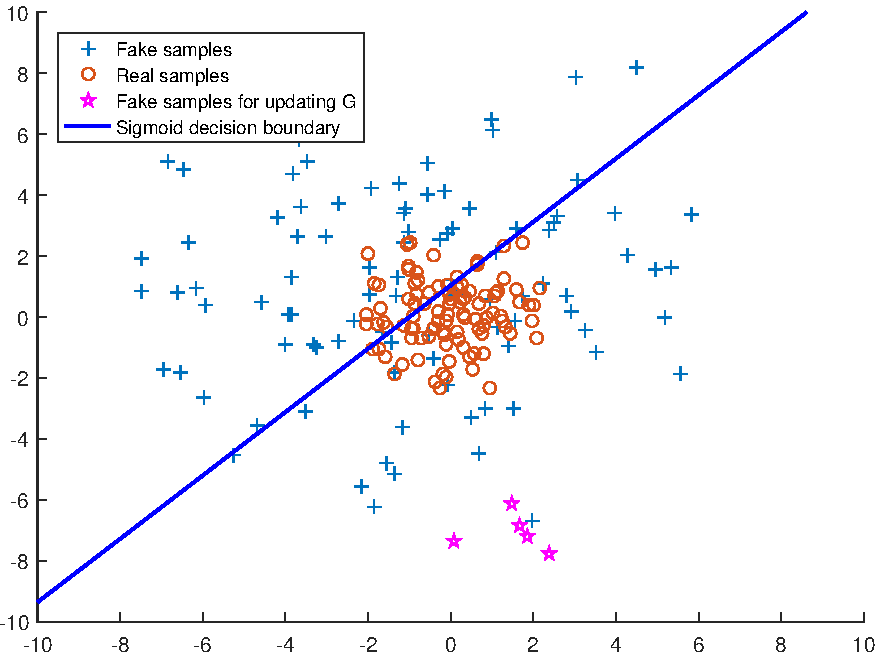
\includegraphics[width=0.95\linewidth]{figures/chapter02/boundary_2.pdf}
        \caption{Límite de decisión de la función de pérdida de entropía cruzada sigmoidea}
        \label{subfig:LSGAN-2}
    \end{subfigure}
    \vspace{0.03\linewidth}
    \begin{subfigure}{.30\linewidth}
        \centering
        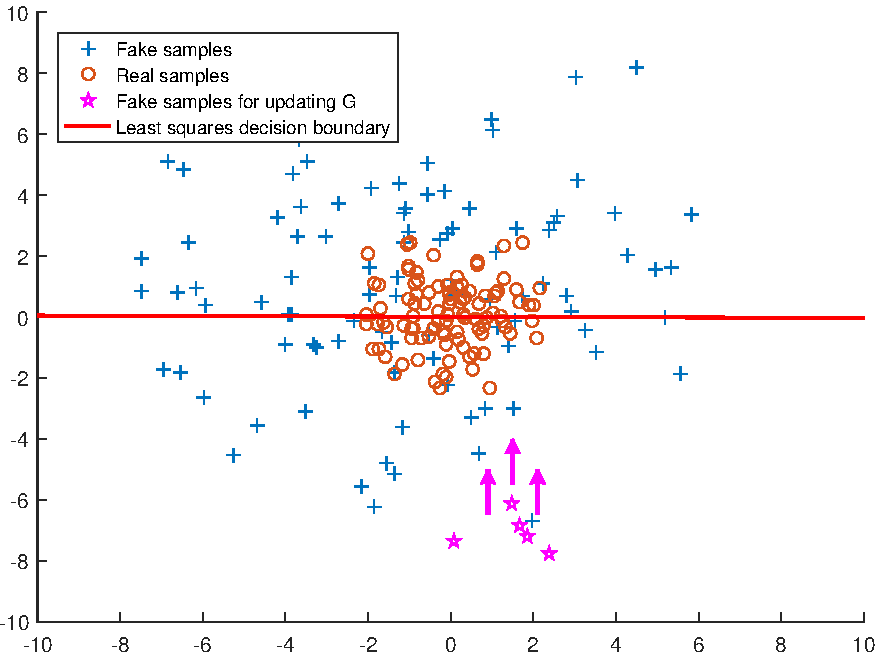
\includegraphics[width=0.95\linewidth]{figures/chapter02/boundary_3.pdf}
        \caption{Límite de decisión de la función de pérdida de mínimos cuadrados.}
        \label{subfig:LSGAN-3}
    \end{subfigure}

    \caption{Least Square Generative Adversarial Network (LSGAN)\newline{}Fuente: Least Squares Generative Adversarial Networks \cite{LSGAN-mao2017squares}}
    \label{fig:LSGAN}
\end{figure}



\subparagraph{Progressive Generative Adversarial Network (ProGAN) [2017]}
% https://paperswithcode.com/method/progan
% https://arxiv.org/abs/1710.10196v3
% https://towardsdatascience.com/explained-a-style-based-generator-architecture-for-gans-generating-and-tuning-realistic-6cb2be0f431

Las redes \gls{ProGAN} o \gls{PGGAN} \cite{ProGAN-karras2018progressive} están basadas en las redes \gls{DCGAN} donde tanto ${G}$ como ${D}$ empiezan con un entrenamiento de imágenes en baja resolución y va aumentando progresivamente la resolución, la idea es hacer que los generadores como los discriminadores vayan aprendiendo progresivamente.

Primero las redes aprenden imágenes de baja resolución ${4 \times 4}$, después ${8 \times 8}$, ${16 \times 16}$, hasta llegar a la resolución, ${1024 \times 1024}$ como vemos en el ejemplo de la Figura \ref{subfig:ProGAN-1}

\begin{figure}[H]
    \centering
    \captionsetup{justification=centering}

    \begin{subfigure}{.475\linewidth}
        \centering
        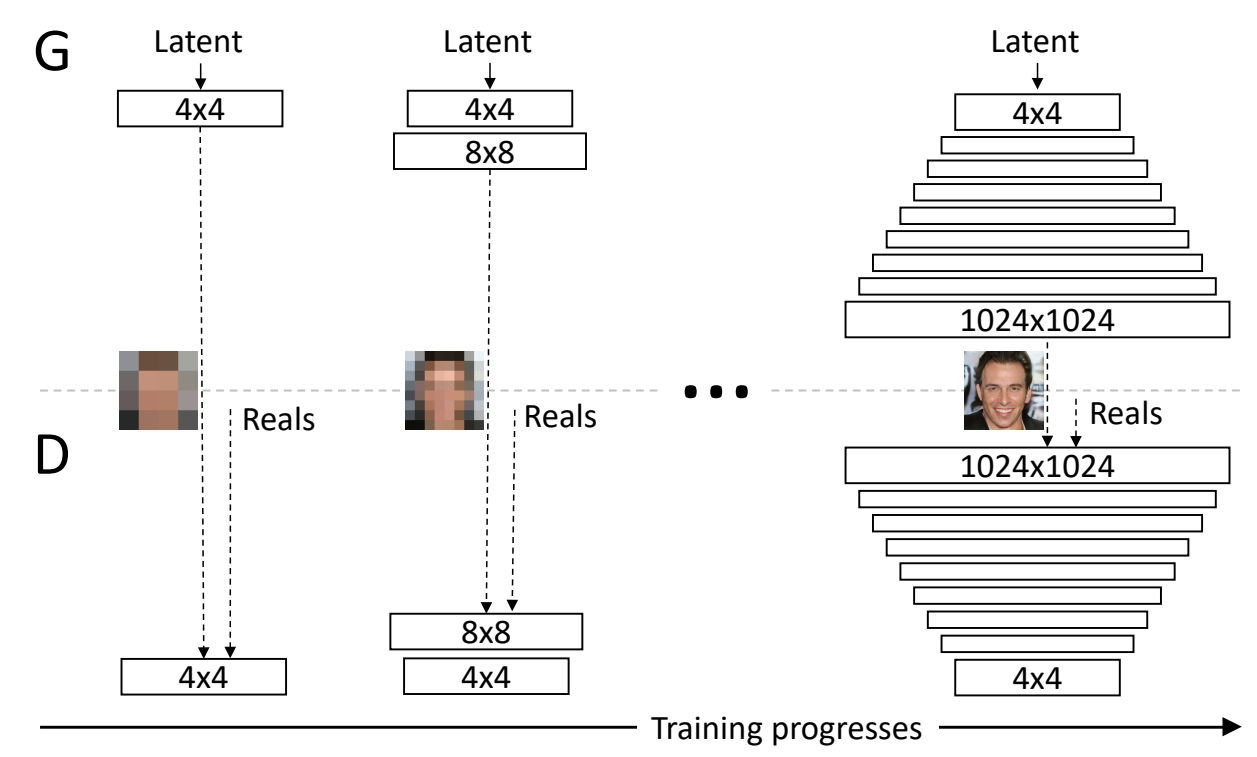
\includegraphics[width=0.75\linewidth]{figures/chapter02/ProGAN-image-32.png}
        \caption{Proceso de entrenamiento de las redes ${G}$ y ${D}$}
        \label{subfig:ProGAN-1}
    \end{subfigure}
    \vspace{0.03\linewidth}
    \begin{subfigure}{.475\linewidth}
        \centering
        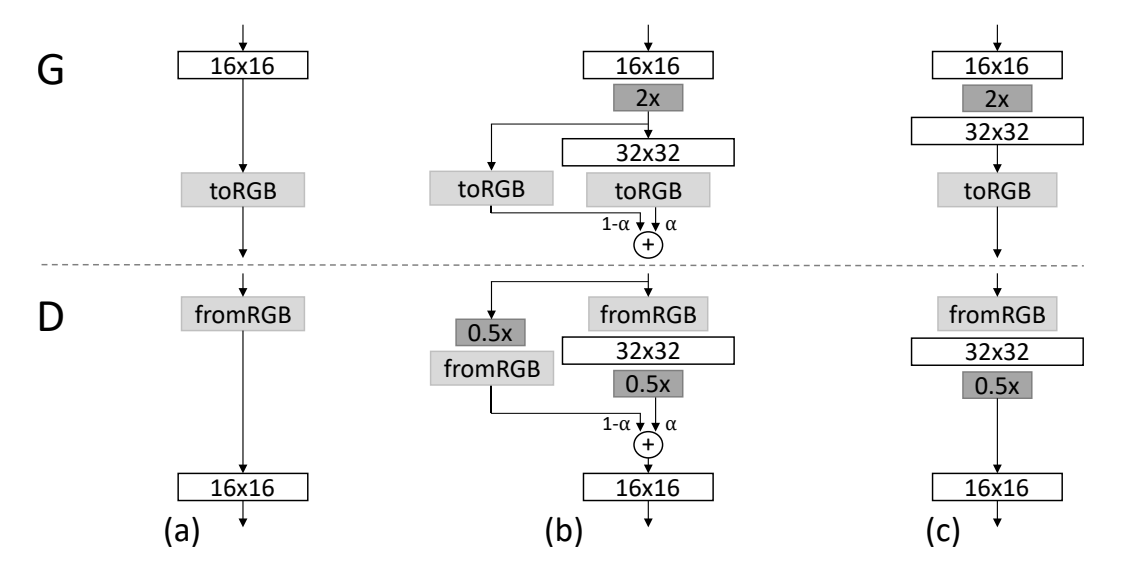
\includegraphics[width=0.75\linewidth]{figures/chapter02/ProGAN-image-16.png}
        \caption{Arquitectura de las redes ${G}$ y ${D}$}
        \label{subfig:ProGAN-2}
    \end{subfigure}

    \caption{Progressive Generative Adversarial Network (ProGAN)\newline{}Fuente: \href{https://blog.paperspace.com/progan/}{ProGAN: Progressive Growing Generative Adversarial Networks}}
    \label{fig:ProGAN}
\end{figure}


\subparagraph{Super Resolution Generative Adversarial Network (SRGAN) [2016]}
% https://paperswithcode.com/method/srgan
% https://arxiv.org/abs/1609.04802
% https://arxiv.org/abs/1711.06491
% https://arxiv.org/abs/1902.06068
% https://homepages.inf.ed.ac.uk/rbf/CVonline/LOCAL_COPIES/VELDHUIZEN/node18.html
Las redes \gls{SRGAN} \cite{SRGAN-ledig2017photorealistic} son una variante de las redes \gls{DCGAN}. Esta red aprende a mapear imágenes de baja resolución a imágenes de alta resolución, utiliza la calidad perceptual en lugar de solo él \gls{PSNR}, estas redes son las que mejores resultados están dando, además de que las abstracciones que aprende no se limitan únicamente al dominio de su entrenamiento sino a la abstracción de formas y patrones en imágenes, estos modelos son sencillos de entrenar y dan buenos resultados.
% TODO

\begin{equation}
    \begin{split}
        \min_{\theta_{G}}\max_{\omega_{D}}~~
        & \mathbb{E}_{I^{H R} {\sim P_{train} (I^{H R})}}  \left[ \log{(D_{\omega_{D}}(I^{H R}))}                      \right]     \\
        & + \mathbb{E}_{I^{L R} {\sim P_{G} (I^{L R})}}    \left[ \log{( 1 - D_{\theta_{D}}(G_{\theta_{G}}(I^{L R})))} \right]     \\
    \end{split}
\end{equation}


\subparagraph{{\small Enhanced Super Resolution Generative Adversarial Network (ESRGAN) [2016]}}
% https://arxiv.org/pdf/1809.00219.pdf
% https://github.com/xinntao/ESRGAN
% https://typeset.io/library/untitled-collection-fu09ijee/esrgan-1809-00219-pdf-3aklgwph
Las redes \gls{ESRGAN} \cite{ESRGAN-wang2018esrgan, SRGAN-ledig2017photorealistic} son una mejora de las \gls{SRGAN}, \gls{ESRGAN} utiliza características antes de la activación para la pérdida perceptual. Esto mejora la consistencia de brillo y la recuperación de texturas. Además, añaden la interpolación de redes para equilibrar la calidad visual y él \gls{PSNR}.

Los investigadores \textit{Xintao Wang, Ke Yu, Shixiang Wu, ...}\cite{ESRGAN-wang2018esrgan} demostraron que las redes \gls{ESRGAN} cuentan con un rendimiento superior a \gls{SRGAN} con un entrenamiento sencillo, contrario a lo que creían los investigadores \textit{Christian Ledig, Lucas Theis, ...} \cite{SRGAN-ledig2017photorealistic} modelos más profundos son más difíciles de entrenar.



\subparagraph{Style Generative Adversarial Network (StyleGAN) [2018]}
% https://paperswithcode.com/method/stylegan
% https://arxiv.org/abs/1812.04948
% https://paperswithcode.com/method/stylegan2
% https://arxiv.org/abs/1912.04958
% Others
% https://arxiv.org/abs/2301.09515

Las redes \gls{StyleGAN} \cite{StyleGAN-karras2019stylebased,StyleGAN-sauer2023stylegant}, es un proyecto desarrollando por NVIDIA, el principal uso de la red es la generación de rostros, actualmente se encuentra en su tercera versión \cite{styleGAN3-karras2021aliasfree}, esta versión cuenta con importantes mejoras de rendimiento, estabilidad, interpolación, entrelazamiento y reducción del \textit{aliasing}. Además, la tercera versión cuenta con la posibilidad de generación de vídeo.

La arquitectura \gls{StyleGAN} \cite{StyleGAN-melnik2023face}, está basada en las redes \gls{PGGAN} que permiten el entrenamiento progresivo, aumentando gradualmente la resolución de las instancias, se introduce la mezcla de estilos de forma distinta a \gls{CycleGAN}, ya que hace un mezclado de los vectores latentes, también añade métodos de inversión con el objetivo de reconstruir vectores latentes de determinadas instancias para manipular editar las instancias en el espacio latente.
% https://towardsdatascience.com/explained-a-style-based-generator-architecture-for-gans-generating-and-tuning-realistic-6cb2be0f431




\subparagraph{Self Attention Generative Adversarial Network (SAGAN) [2018]}
% https://arxiv.org/abs/1805.08318
% https://paperswithcode.com/method/sagan
En las redes \gls{SAGAN} \cite{SAGAN-zhang2018selfattention} permiten modelar dependencias de largo alcance usando técnicas de atención para tareas de generación de imágenes.
Estas redes permiten generar más detalles usando pistas del mapa de características, la red ${D}$ puede comprobar que los rasgos detallados de las instancias generadas son coherentes entre sí.



\subparagraph{Wasserstein Generative Adversarial Network (WGAN) [2017]}
% https://lilianweng.github.io/posts/2017-08-20-gan/
% https://neptune.ai/blog/gan-loss-functions
% https://arxiv.org/abs/1701.07875
% https://paperswithcode.com/method/wgann
% https://medium.com/@mladenkorunoski/wgans-explained-fab61bda2576
Las redes \gls{WGAN} \cite{WGAN-arjovsky2017wasserstein, WGAN-weng2017gan, WGAN-weng2019gan} se basan en la arquitectura clásica de una red \gls{GAN}, pero modifican el discriminador con la intención de que los modelos converjan, esta arquitectura utiliza la distancia de Wasserstein\footnote{La distancia de Wasserstein mide cuánto ``movimiento'' se necesita para transformar una distribución en otra. En términos simples, es como medir la cantidad de trabajo necesario para mover tierra de un lugar a otro.} como función de perdida, esto busca mejorar la estabilidad del entrenamiento y la calidad de las instancias generadas, además evita problemas de colapso de modo\footnote{Durante el entrenamiento, un generador puede ``colapsar'' a una configuración en la que siempre produce las mismas salidas.}.

% Puedes consultar el teorema \ref{theorem::gradW}.

\subparagraph{Wasserstein Generative Adversarial Network with Gradient Penalty (WGAN-GP) [2017]}
% https://neptune.ai/blog/gan-loss-functions
% https://arxiv.org/abs/1701.07875
% https://paperswithcode.com/method/wgan-gp
% https://eva.fing.edu.uy/pluginfile.php/362486/mod_resource/content/3/WGANs.pdf

Las redes \gls{WGAN-GP} \cite{WGAN-GP-gulrajani2017improved} basadas en la arquitectura de las redes \gls{WGAN}, añaden un factor de penalización, mejorando considerablemente la estabilidad del modelo.

Al agregar esta penalización de gradiente, mejora la suavidad en la función de pérdida lo que ayuda a la estabilidad, la penalización, también se recortan los pesos esto ayuda a mantener controlado la continuidad de \textit{Lipschitz} en el discriminador con lo que el modelo converge a una solución más realista.





\subparagraph{Information Maximizing Generative Adversarial Network (InfoGAN) [2016]}
% https://arxiv.org/pdf/1606.03657.pdf
% https://arindam.cs.illinois.edu/courses/f21cs598/slides/gan11_598f21.pdf

% la red generativa ${G}$, se encuentra condicionada de la siguiente forma ${G(z\mid{}c)}$.
Las redes \gls{InfoGAN} \cite{InfoGAN-chen2016infogan}, introduce un discriminador adicional llamado ${Q}$ o red de reconocimiento para controlar las características de las instancias, es la  responsable de estimar los códigos latentes a partir de las instancias generadas. La función objetivo de las redes \gls{InfoGAN} es la regularización de la función objetivo de las \gls{cGAN}. Esto permite controlar la red neuronal de forma que la podamos condicionar a que genere instancias de un dominio y que las instancias generadas contengan ciertas características.

La arquitectura lo logra usando la red ${Q}$ con dos estructuras, una para controlar las variables discretas y otra para las variables continuas del ruido latente, estas variables se utilizan para el cálculo de la perdida. Con esto logra controlar que las instancias generadas sean válidas y coherentes con las clases y características.

\begin{figure}[H]
    \centering
    \centerline{\includesvg[width=0.99\columnwidth]{figures/chapter02/GANs-InfoGAN.drawio.svg}}
    \caption{Arquitectura Information Maximizing GAN (InfoGAN).\newline{}Fuente: Elaboración propia.}
    \label{fig:InfoGAN}
\end{figure}

La arquitectura de \gls{InfoGAN} diferencia entre las redes ${G}$, ${D}$ y ${Q}$, aunque ${D}$ y ${Q}$ comparten la misma arquitectura de red, solo se diferencia en las unidades de salida en la última capa, esto hace que el coste de entrenamiento del modelo sea levemente superior a una red \gls{GAN} clásica, pero con importantes mejoras.

    {\small
        \begin{equation}
            \begin{split}
                \min_{G,Q}\max_{D} V_{InfoGAN}(D,G,Q)   &= V(G,D) - \lambda I(G,Q)      \\
                \min_{G}\max_{D} V_{InfoGAN}(D,G)       &= V(G,D) - \lambda I(c;G(z,c)) \\
            \end{split}
            \label{eq:InfoGAN}
        \end{equation}
    }

${I(c;x)}$ es la información mutua y mide cuanto se sabe de ${c}$ si conocemos ${x}$, es decir si la instancia de $x$ es completamente irrelevante a ${c}$, entonces el discriminador indicara ${I(c;x) = 0}$.

    {\small
        \begin{equation}
            \begin{split}
                I(c; G(z,c))    &=  H(c) - H(c \mid G(z,c))     \\
                &=  H(c) - \mathbb{E}_{x\sim{}G(z,c)}\left[\mathbb{E}_{c'\sim{}P_{c\sim{}x}} \left[ \log{P(c'\mid{}x)}\right]\right]
            \end{split}
        \end{equation}
    }

En el artículo \textit{Interpreting the Latent Space of GANs for Semantic Face Editing} \cite{GANLatentSpace-shen2020interpreting} se propone un método para la interpretación semántica codificada en el espacio latente, esto permite controlar las características de las instancias generadas.



% \subparagraph{Secure Steganography Generative Adversarial Network (SSGAN) [2017]}
% https://arxiv.org/abs/1707.01613
% Las redes \gls{SSGAN} \cite{SSGAN-shi2018ssgan}

% ~V_{SSGAN}(G,D,S)~=~
% \begin{equation}
%     \begin{split}
%         \min_{G}\max_{D}\max_{S}
%         &= \alpha       \left[\mathbb{E}_{x\sim{}P_{\text{data}}(x)} \log(D(x)) + \mathbb{E}_{z\sim{}P_{\text{noise}}(z)} \log(1 - D(G(z)))   \right] \\
%         &+ (1 - \alpha) \left[\mathbb{E}_{z\sim{}P_{\text{noise}}(z)}\log\left( S(\mathrm{Stego}(G(z)))\right)   + \log(1 - S(G(z)))   \right]
%     \end{split}
% \end{equation}


% OTRAS
% https://github.com/jasonshere/FairGAN

\subsubsection{Inversión de GANs}
\label{ch:2:GAN-inversion}
% https://sertiscorp.medium.com/gan-inversion-a-brief-walkthrough-part-i-bc2ee1b73253
% https://sertiscorp.medium.com/gan-inversion-a-brief-walkthrough-part-ii-e192513b89ae
% https://sertiscorp.medium.com/gan-inversion-a-brief-walkthrough-part-iii-da87c28f9e62
% https://sertiscorp.medium.com/gan-inversion-a-brief-walkthrough-part-iv-a72bc713e3c8

Como se especifica en el artículo \cite{GANInversionSurvey-xia2022gan} el generador aprende patrones en el espacio de distribución. Este espacio ${N-\text{dimensional}}$ es el código latente con las características del dominio, se le denomina ${z}$. La inversión de \gls{GAN} proporciona una relación del espacio latente para obtener el código latente del dominio.

El objetivo de la inversión \gls{GAN} es el de obtener el vector latente para cualquier instancia determinada. La obtención de este vector latente proporciona flexibilidad para realizar manipulación de instancias reales en vez de solo poder manipular instancias generadas.

La \gls{GAN} Inversión tiene múltiples aplicaciones, destaca en la manipulación, generación, restauración e interpolación de instancias. Así como en la reconstrucción 3D, comprensión de las instancias, aprendizaje multimodal o imágenes médicas \cite{GANInversionSurvey-xia2022gan}.

\begin{figure}[H]
    \centering
    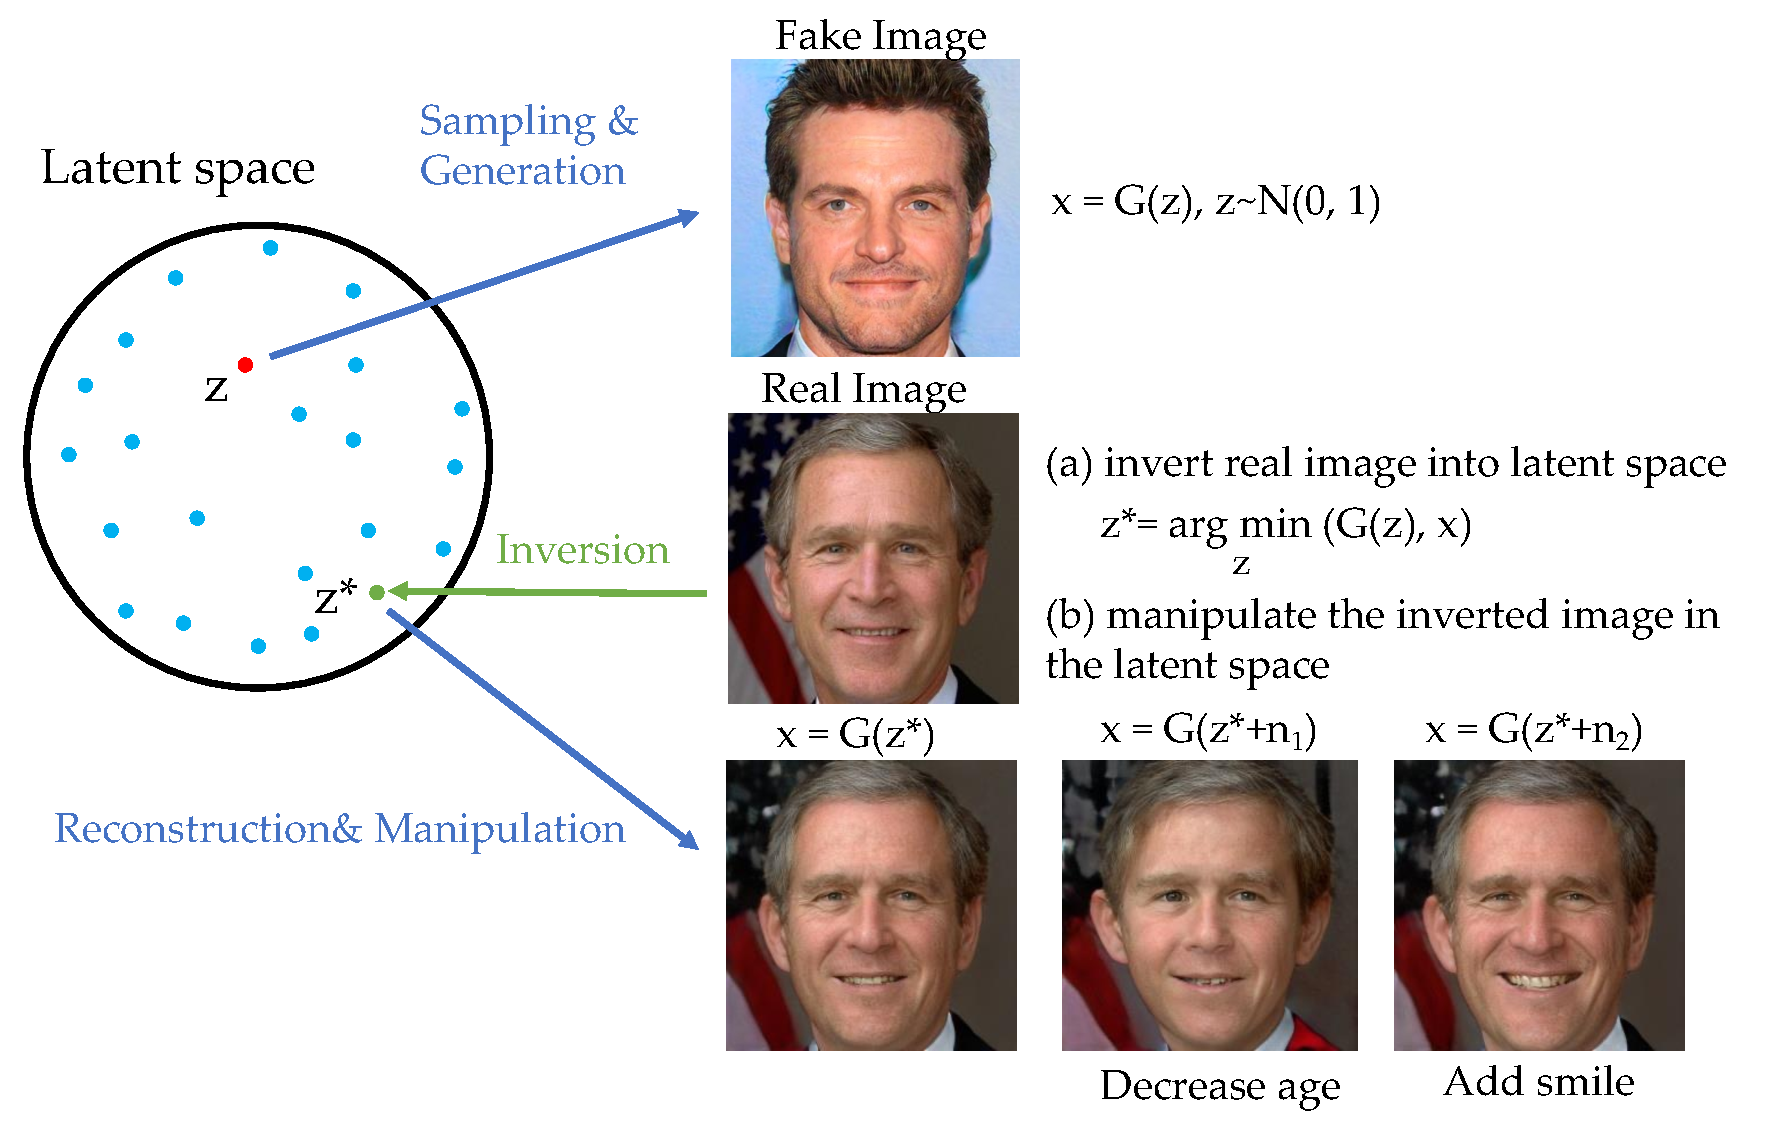
\includegraphics[width=0.5\linewidth]{figures/chapter02/overview.pdf}
    \caption{Ilustración de la inversión de GAN.\newline{}Fuente: GAN Inversion: A Survey \cite{GANInversionSurvey-xia2022gan}}
    \label{fig:gan-inversion}
\end{figure}

Este problema está definido formalmente \ref{eq:inversion-problem-objective-function} como una función objetivo.

\begin{equation}
    z^{*} = \underset{z}{\arg\min}\, \ell\left( G(z), x \right),
    \label{eq:inversion-problem-objective-function}
\end{equation}

A continuación, en la Figura \ref{fig:gan-inversion-methods} se presentan el flujo para la extracción del vector del código latente de los distintos métodos que han propuesto en el artículo \cite{GANInversionSurvey-xia2022gan}.

\begin{figure}[H]
    \centering
    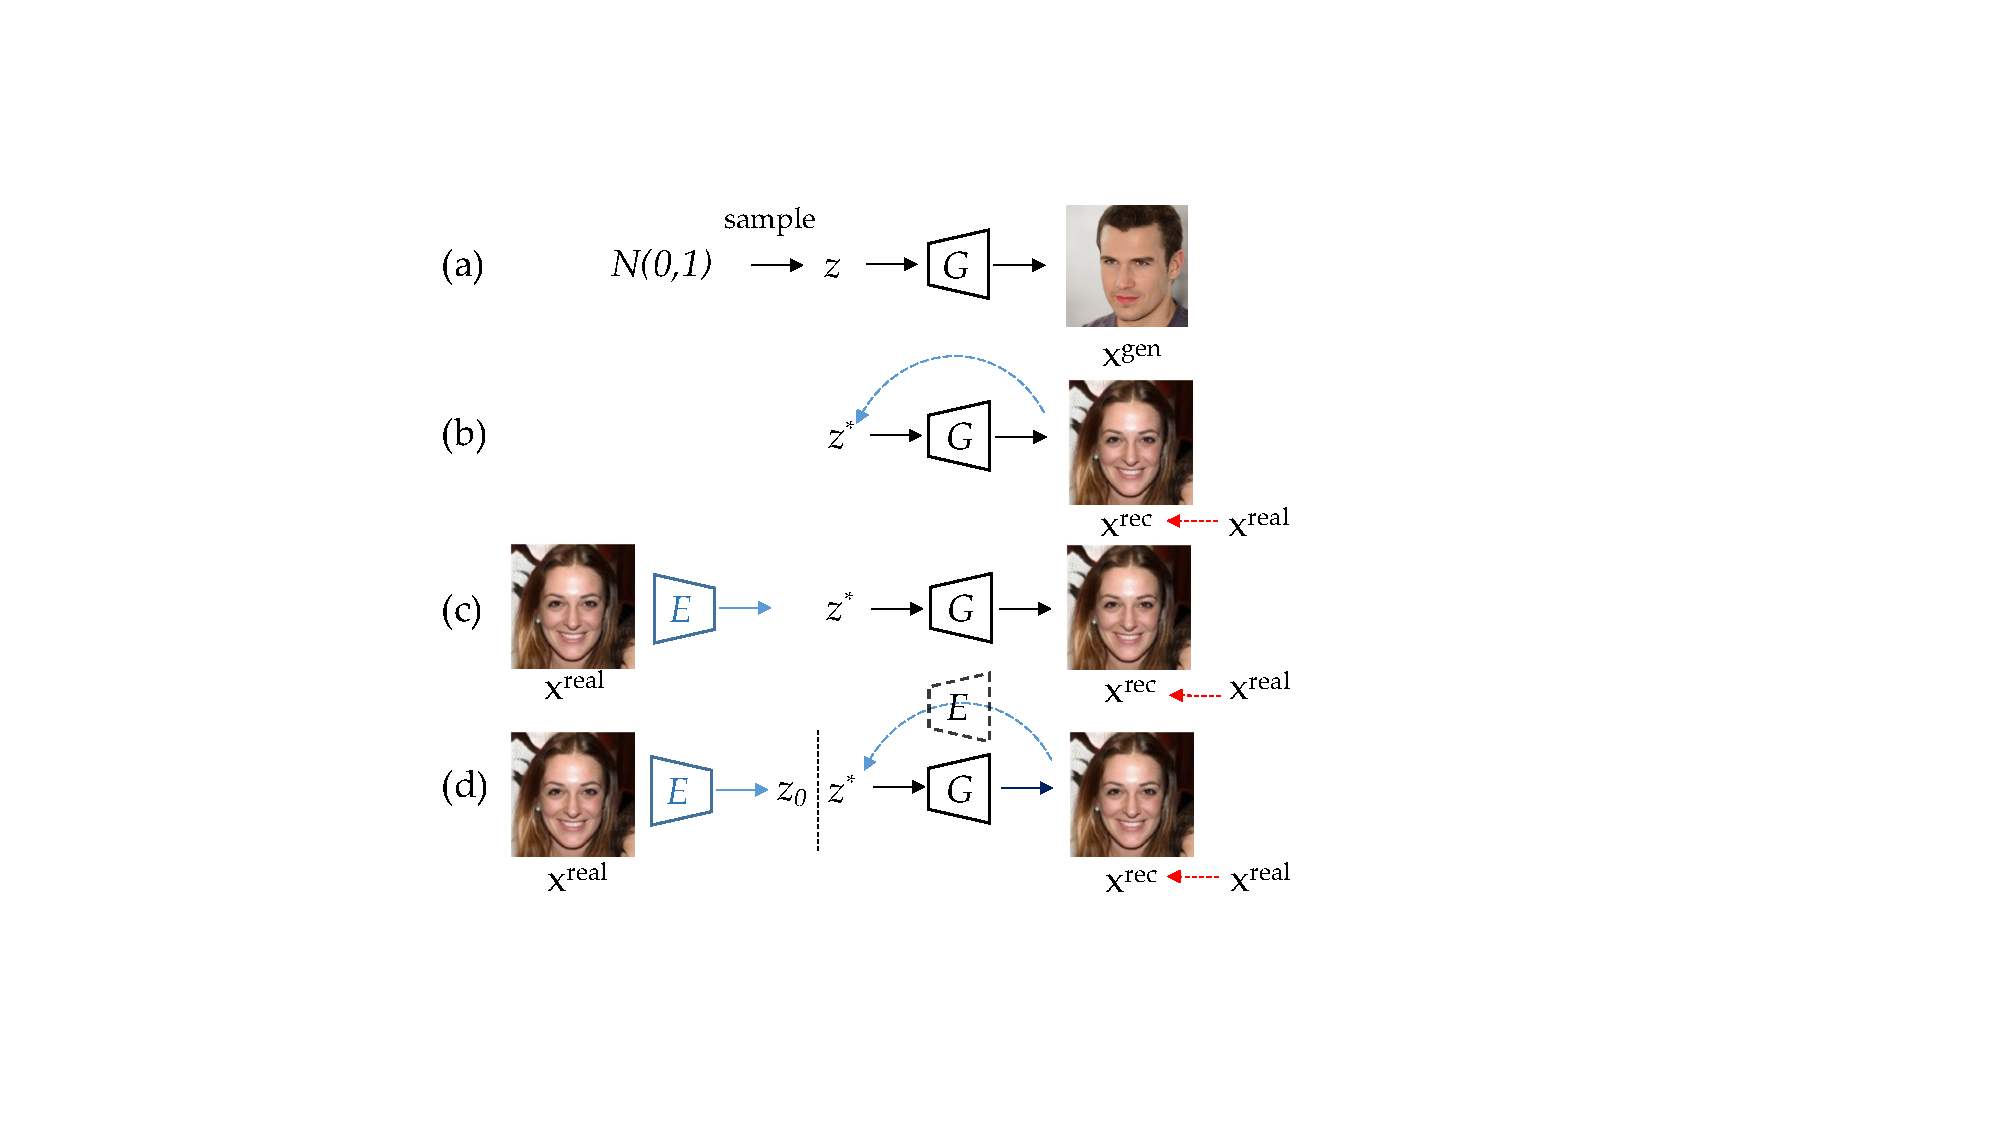
\includegraphics[width=0.5\linewidth]{figures/chapter02/inversion_types.pdf}
    \caption{Tipos de GAN inversión.\newline{}Fuente: GAN Inversion: A Survey \cite{GANInversionSurvey-xia2022gan}}
    \label{fig:gan-inversion-methods}
\end{figure}

En la sección \textbf{a} de la Figura \ref{fig:gan-inversion-methods} podemos observar una \gls{GAN} clásica sin ningún método de inversión.

En la sección \textbf{b} de la Figura \ref{fig:gan-inversion-methods} podemos ya ver el método \textit{Optimization-based} optimiza el vector latente ${z}$ para reconstruir una imagen ${x^{\text{rec}}}$ cercana a la instancia real ${x}$. La función objetivo es la definida en la ecuación \ref{eq:GAN-inversion--optimization-based}.

\begin{equation}
    z^{*} = \underset{z}{\arg\min}\, \ell(x, G(z; \theta))
    \label{eq:GAN-inversion--optimization-based}
\end{equation}

En la sección \textbf{c} de la Figura \ref{fig:gan-inversion-methods} podemos observar el método \textit{Learning-based} que incorpora un módulo codificador llamado ${E}$ que se entrena utilizando instancias generadas por ${G}$ con sus vectores latentes. Es decir, el codificador ${E}$ intenta generar un vector latente denominado ${z_{n}}$ para la instancia ${x_{n}}$ tal que cuando el vector latente se pase a la red ${G}$. La función objetivo es la definida en la ecuación \ref{eq:GAN-inversion--learning-based}.

\begin{equation}
    {\theta}_{E}^{*} = \underset{\theta_{E}}{\arg\min} \sum_{n}{ \mathcal{L}(G(E(x_{n};\theta_{E})),x_{n})  }
    \label{eq:GAN-inversion--learning-based}
\end{equation}

En la sección \textbf{d} de la Figura \ref{fig:gan-inversion-methods} podemos observar el método \textit{Hybrid-based} que incorpora los enfoques \textit{Optimization} y \textit{Learning}. Durante la inferencia, la instancia real ${x}$ se pasa al codificador ${E}$ con el que se obtiene ${z}$, este valor será la inicialización ${z_{0}}$ del vector latente de optimización para reducir la distancia entre la instancia real ${x}$ y la instancia reconstruida ${x^{\text{rec}}}$

\subparagraph{Aplicaciones de la inversión de GANs}

Algunos investigadores han estudiado la inversión de GANs para diseccionar GANs y comprender sus abstracciones internas, esto también sirve para entender qué características las GANs no aprenden.

\textbf{Interpolación de instancias}:
Una posibilidad es usar una interpolación lineal en el espacio latente, con ello podemos fusionar dos vectores latentes en el espacio latente, esto logra una transición suave

\begin{equation}
    \mathrm{z} = \mathrm{z}_{1}(\lambda) + \mathrm{z}_{2}(1 - \lambda) ~\text{donde}~ \lambda \in (0,1)
\end{equation}

Nos referimos como ${\mathrm{z}}$ al vector latente de la interpolación de las dos instancias ${\mathrm{z}_{1}}$ y ${\mathrm{z}_{2}}$ y ${\alpha}$ es el factor de paso

\textbf{Manipulación de instancias}:
Mediante una transformación lineal en el espacio latente, se puede lograr una manipulación de las instancias, esto se logra transformando el código latente de la imagen en direcciones semánticas específicas.

\begin{equation}
    \begin{split}
        \mathrm{x}^{\prime} &= G(\mathrm{z}^{\prime}) \\
        \mathrm{z}^{\prime} &= \mathrm{z} + \alpha ~n
    \end{split}
\end{equation}

Nos referimos como ${\mathrm{z}^{\prime}}$ y ${\mathrm{x}^{\prime}}$ al código latente manipulado de la instancia, ${\alpha}$ es el factor de paso y ${n}$ es la dirección semántica específica del espacio latente.

\textbf{Difusión semántica}:
De forma similar a \textit{Context Encoder} se hace un recorte de la instancia para fusionar junto con otra instancia recortada y difuminar la fusión de ambas instancias, el objetivo es que la instancia generada conserve las características de la imagen destino.

\begin{figure}[H]
    \captionsetup[subfigure]{justification=centering}
    \begin{subfigure}{.60\linewidth}
        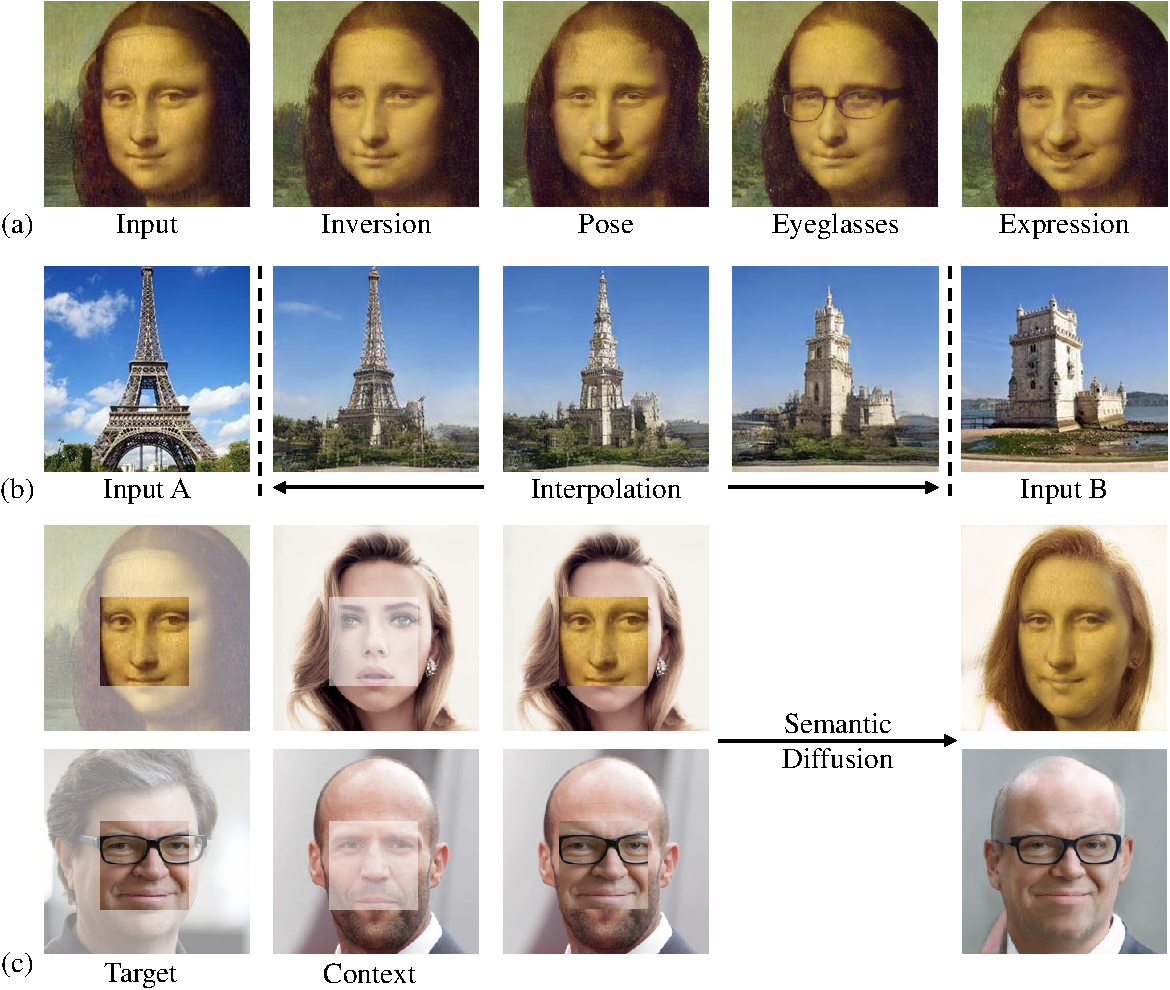
\includegraphics[width=\linewidth]{figures/chapter02/main_teaser.pdf}
        \caption{Difusión semántica}
        \label{subfig:semantic-diffusion}
    \end{subfigure} 
    \hfill
    \begin{subfigure}{.35\linewidth}
        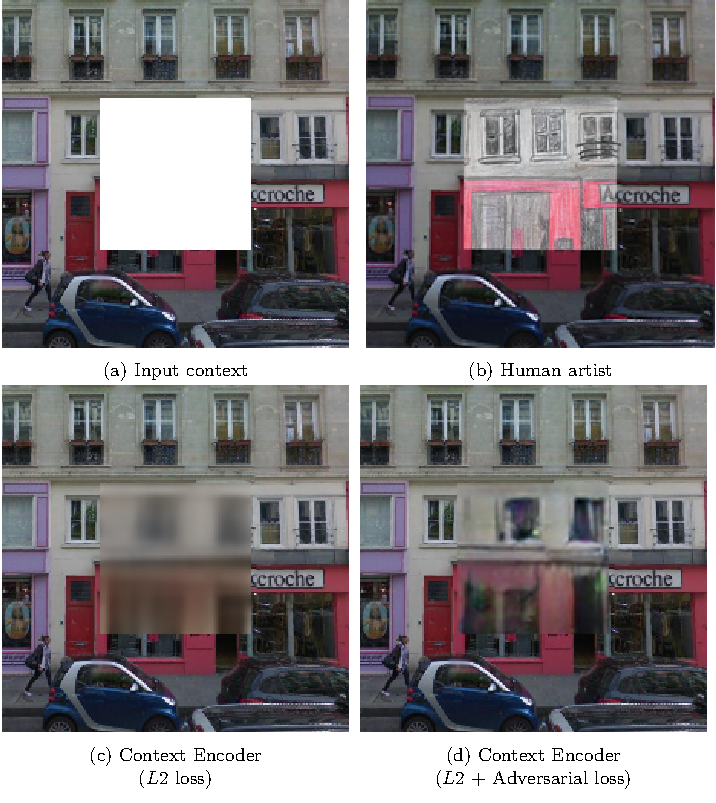
\includegraphics[width=\linewidth]{figures/chapter02/context-encoder.pdf}
        \caption{Context Encoder}
        \label{subfig:context-encoder}
    \end{subfigure}

    \caption{Diferencias entre Difusión semántica y Context Encoder}
    \label{fig:context-encoder-vs-semantic-diffuson}
\end{figure}



% endregion Redes generativas adversariales

\subsection{La seguridad de las redes neuronales} 
\label{ch:2:section:state-of-the-art:computer-security-in-neural-networks}
% region subsection La seguridad de las redes neuronales
% TODO: 
% https://ieeexplore.ieee.org/stamp/stamp.jsp?tp=&arnumber=9294026
% Dentro de la inteligencia artificial \gls{AI} encontramos el aprendizaje automático \gls{ML} y dentro el aprendizaje profundo \gls{DL}.
% Para el desarrollo de este capítulo limitaremos el alcance del estado del arte de la seguridad informática a los campos relacionados con la inteligencia artificial.

El estado del arte de la seguridad informática es muy complejo, ya que los delincuentes informáticos adoptan nuevas técnicas y tácticas para eludir las medidas de seguridad, esto hace que las amenazas informáticas estén en constante evolución, también amenaza a las tecnologías que emplean la inteligencia artificial y redes neuronales.

A continuación, se explicarán las distintas amenazas que tiene una red neuronal y como puede ser atacada o implementar defensas, posteriormente analizaremos el estado del arte de la inteligencia artificial que se emplea para mejorar la seguridad informática de los dispositivos y de los usuarios.

La librería \texttt{ART} \cite{art2018}, es una librería de \texttt{Python} especializada en la seguridad del \gls{ML}, \texttt{ART} proporciona herramientas que permiten a los desarrolladores e investigadores evaluar modelos de aprendizaje automático, la librería se especializa en amenazas de evasión, encantamento, extracción e inferencia. La librería consta con 6 módulos específicos para ataque, defensas, estimadores, evaluaciones, métricas y pre-procesamiento. Esto podemos verlo en la Figura \ref{fig:art-architecture}.

\begin{figure}[H]
    \centering
    \centerline{\includesvg[width=0.99\linewidth]{figures/chapter02/art-architecture.drawio.svg}}
    \caption{Arquitectura de ART.\newline{}Fuente: \href{https://github.com/Trusted-AI/adversarial-robustness-toolbox/wiki/ART-Architecture-and-Roadmap}{GitHub @Trusted-AI/adversarial-robustness-toolbox}}
    \label{fig:art-architecture}
\end{figure}

Los modelos profundos ofrecen mejoras notables, aunque sin las consideraciones de seguridad pueden ser que nuestros modelos se vean amenazados por la injerencia de terceros

Como podemos observar en la Figura \ref{fig:art-adversarial-threats} existen multitud de amenazas, existen cuatro formas de clasificar las amenazas, esta clasificación es en función de cómo se altera el comportamiento del modelo.

\begin{figure}[H]
    \centering
    \centerline{\includesvg[width=0.99\columnwidth]{figures/chapter02/adversarial-threats.drawio.svg}}
    \caption{Amenazas en redes neuronales.\newline{}Fuente: Elaboración propia.}
    \label{fig:art-adversarial-threats}
\end{figure}

% Eficiencia
% Invisivilidad
% Efectividad

% endregion subsection La seguridad de las redes neuronales

% ===================================
% ===================================
\subsection{Ataques en \textit{deep learning}}
% region subsection Ataques en \textit{deep learning}

Los modelos de inteligencia artificial presentan una serie de ventajas muy interesantes, sobre todo para un atacante, ya que si se conoce el modelo que emplea puede ser viable la perturbación del modelo con el objetivo de alterar el comportamiento o los resultados.

A continuación se muestra los posibles vectores de ataque que se pueden ejecutar sobre los modelos, se trata de una recopilación de todos los artículos científicos más relevantes del momento.
 
 % \begin{figure}[H]
 %     \centering
 %    \centerline{\includesvg[width=0.50\columnwidth]{figures/chapter02/taxonomia-deep-learning-ataques.drawio}}
 %     \caption{Texonomia Deep Learning - Attack}
 %     \label{fig:tax-deep-learning-attack}
 % \end{figure}

% endregion subsection Ataques en \textit{deep learning}

\subsubsection{Evasión}
% region subsubsection Evasión
Busca explotar las vulnerabilidades de la red neuronal para inducir errores en la capacidad de clasificar o de predecir. Se envía información con perturbaciones mínimas que alteren notablemente la respuesta del modelo.

\clearpage
\paragraph{White Box}
Se conoce todo sobre el modelo, arquitectura, pesos, umbrales, formato de entrada de datos y salida, etc. \cite{learning-machine-learning-part-3-attacking}

Uno de los primeros ataques de evasión que se publicaron fue el de \gls{FGM} de \textit{Ian J. Goodfellow} en 2014 \cite{goodfellow2015explaining}

%     \begin{tblr}{hlines,vlines,rows={valign=m},row{1}={c},colspec={Q[m]X}} 


\begin{longtblr}[caption={Lista de ataques de caja blanca}, label={tab:my-table-white-box}]{hlines, vlines, rows={valign=m}, row{1}={c}, colspec={XX},  cells = {font = \fontsize{10pt}{12pt}\selectfont}} 
    \textbf{Título}                                                                            & \textbf{Referencias}                                                                                                                                                                               \\ 
    Auto Projected Gradient Descent (Auto-PGD)                                                 & \href{https://arxiv.org/abs/2003.01690}{(Croce and Hein, 2020)}                                                                                                                                    \\ 
    Shadow Attack                                                                              & \href{https://arxiv.org/abs/2003.08937}{(Ghiasi et al., 2020)}                                                                                                                                     \\ 
    Wasserstein Attack                                                                         & \href{https://arxiv.org/abs/1902.07906}{(Wong et al., 2020)}                                                                                                                                       \\ 
    PE Malware Attacks                                                                         & \href{https://arxiv.org/abs/1810.08280}{(Suciu et al., 2018)}, \href{https://arxiv.org/abs/2008.07125}{(Demetrio et al., 2020)}, \href{https://arxiv.org/abs/1901.03583}{(Demetrio et al., 2019)}  \\ 
    Imperceptible, Robust, and Targeted Adversarial Examples for Automatic Speech Recognition  & \href{https://arxiv.org/abs/1903.10346}{(Qin et al., 2019)}                                                                                                                                        \\ 
    Brendel \& Bethge Attack                                                                   & \href{https://arxiv.org/abs/1907.01003}{(Brendel et al., 2019)}                                                                                                                                    \\ 
    Targeted Universal Adversarial Perturbations                                               & \href{https://arxiv.org/abs/1911.06502}{(Hirano and Takemoto, 2019)}                                                                                                                               \\ 
    Audio Adversarial Examples: Targeted Attacks on Speech-to-Text                             & \href{https://arxiv.org/abs/1801.01944}{(Carlini and Wagner, 2018)}                                                                                                                                \\ 
    High Confidence Low Uncertainty (HCLU) Attack                                              & \href{https://arxiv.org/abs/1812.02606}{(Grosse et al., 2018)}                                                                                                                                     \\ 
    Iterative Frame Saliency                                                                   & \href{https://arxiv.org/abs/1811.11875}{(Inkawhich et al., 2018)}                                                                                                                                  \\ 
    DPatch                                                                                     & \href{https://arxiv.org/abs/1806.02299v4}{(Liu et al., 2018)}                                                                                                                                      \\ 
    Robust DPatch                                                                              & \href{https://arxiv.org/abs/1806.02299v4}{(Liu et al., 2018)}, \href{https://arxiv.org/abs/1906.11897}{(Lee and Kolter, 2019)}                                                                     \\ 
    ShapeShifter                                                                               & \href{https://arxiv.org/abs/1804.05810}{(Chen et al., 2018)}                                                                                                                                       \\ 
    Projected Gradient Descent (PGD)                                                           & \href{https://arxiv.org/abs/1706.06083}{(Madry et al., 2017)}                                                                                                                                      \\ 
    NewtonFool                                                                                 & \href{http://doi.acm.org/10.1145/3134600.3134635}{(Jang et al., 2017)}                                                                                                                             \\ 
    Elastic Net                                                                                & \href{https://arxiv.org/abs/1709.04114}{(Chen et al., 2017)}                                                                                                                                       \\ 
    Adversarial Patch                                                                          & \href{https://arxiv.org/abs/1712.09665}{(Brown et al., 2017)}                                                                                                                                      \\ 
    Decision Tree Attack                                                                       & \href{https://arxiv.org/abs/1605.07277}{(Papernot et al., 2016)}                                                                                                                                   \\ 
    Carlini \& Wagner (C\&W) ${\ell_{2}}$ and ${\ell_{\infty}}$ attack                         & \href{https://arxiv.org/abs/1608.04644}{(Carlini and Wagner, 2016)}                                                                                                                                \\ 
    Basic Iterative Method (BIM)                                                               & \href{https://arxiv.org/abs/1607.02533}{(Kurakin et al., 2016)}                                                                                                                                    \\ 
    Jacobian Saliency Map                                                                      & \href{https://arxiv.org/abs/1511.07528}{(Papernot et al., 2016)}                                                                                                                                   \\ 
    Universal Perturbation                                                                     & \href{https://arxiv.org/abs/1610.08401}{(Moosavi-Dezfooli et al., 2016)}                                                                                                                           \\ 
    Feature Adversaries                                                                        & \href{https://arxiv.org/abs/1511.05122}{(Sabour et al., 2016)}                                                                                                                                     \\ 
    DeepFool                                                                                   & \href{https://arxiv.org/abs/1511.04599}{(Moosavi-Dezfooli et al., 2015)}                                                                                                                           \\ 
    Virtual Adversarial Method                                                                 & \href{https://arxiv.org/abs/1507.00677}{(Miyato et al., 2015)}                                                                                                                                     \\ 
    Fast Gradient Method                                                                       & \href{https://arxiv.org/abs/1412.6572}{(Goodfellow et al., 2014)}                                                                                                                                  \\ 
\end{longtblr}

\paragraph{Black Box}
Se desconoce el modelo, arquitectura, pesos, umbrales, pero se conoce el formato de entrada de datos y la respuesta del modelo. \cite{learning-machine-learning-part-3-attacking}

\begin{table}[H]
    \centering
    \footnotesize
    \begin{tblr}{hlines, vlines, rows={valign=m}, row{1}={c}, colspec={XX},  cells = {font = \fontsize{10pt}{12pt}\selectfont}} 
        \textbf{Título }                            & \textbf{Referencias}                                                                                                                                      \\
        Square Attack                               & \href{https://arxiv.org/abs/1912.00049}{(Andriushchenko et al., 2020)}                                                                                    \\
        HopSkipJump Attack                          & \href{https://arxiv.org/abs/1904.02144}{(Chen et al., 2019)}                                                                                              \\
        Threshold Attack                            & \href{https://arxiv.org/abs/1906.06026}{(Vargas et al., 2019)}                                                                                            \\
        Pixel Attack                                & \href{https://arxiv.org/abs/1906.06026}{(Vargas et al., 2019)}, \href{https://ieeexplore.ieee.org/abstract/document/8601309/citations}{(Su et al., 2019)} \\
        Simple Black-box Adversarial (SimBA)        & \href{https://arxiv.org/abs/1905.07121}{(Guo et al., 2019)}                                                                                               \\
        Spatial Transformation                      & \href{https://arxiv.org/abs/1712.02779}{(Engstrom et al., 2017)}                                                                                          \\
        Query-efficient Black-box                   & \href{https://arxiv.org/abs/1712.07113}{(Ilyas et al., 2017)}                                                                                             \\
        Zeroth Order Optimisation (ZOO)             & \href{https://arxiv.org/abs/1708.03999}{(Chen et al., 2017)}                                                                                              \\
        Decision-based/Boundary Attack              & \href{https://arxiv.org/abs/1712.04248}{(Brendel et al., 2018)}                                                                                           \\
        Geometric Decision-based Attack (GeoDA)     & \href{https://arxiv.org/abs/2003.06468}{(Rahmati et al., 2020)}                                                                                           \\
    \end{tblr}
    \caption{Lista de ataques de caja negra}
    \label{tab:my-table-black-box}
\end{table}

% endregion subsubsection Evasión

\subsubsection{Envenenamiento}
% region subsubsection Envenenamiento

Los atacantes intentan manipular los datos de entrenamiento con el objetivo de influir en el resultado del aprendizaje del modelo, esto pueden hacerlo desde distintas etapas.

Estos ataques inyectan datos de entrenamiento especialmente diseñados que aumentan el error. Los ataques de envenenamiento se centran en el hecho de que la mayoría de los algoritmos de aprendizaje asumen que sus datos tienen una distribución natural, esto puede no cumplirse en entornos que no cumplan las medidas de seguridad. \cite{biggio2013poisoning}

Existen los ataques de puerta trasera, es decir, modelos profundos que tienen un comportamiento normal, pero que dado un dato o una secuencia de entrada dispara un comportamiento malicioso, esto puede hacer que el modelo tenga un comportamiento normal en la mayoría de casos, pero que dada determinada secuencia puede deteriorar enormemente el rendimiento del modelo. \cite{gu2019badnets}

Estos ataques de puerta trasera logran muy buenos resultados sesgando el conjunto de datos de forma muy limitada, consiguen una tasa de error del 92\% con una tasa de envenenamiento de solo el 5\% \cite{cheng2023attacking}.

En el artículo \cite{tan2020bypassing} trata de como evitar la detección de los ataques de puerta trasera. En el artículo se diseña un algoritmo de entrenamiento adversario adaptativo que optimiza la función de pérdida original del modelo y también maximiza la indistinguibilidad de las representaciones ocultas de datos envenenados y datos limpios.

En la sección Defensas en Deep Learning \ref{sec:defense} entraremos en detalle de como nos podemos defender a estos ataques, es decir, detectar los ataques de puerta trasera.

El artículo \cite{saha2019hidden} de 2019 tratan de ocultar el disparador de puerta trasera. En propuestas previas, los datos envenenados o los disparadores se podían identificar mediante una inspección visual, en el artículo proponen una forma novedosa de ataque de puerta trasera donde los datos envenenados parecen naturales con etiquetas correctas y el disparador está oculto en los datos envenenados, con esto logra mantener el ataque oculto hasta el momento de la prueba.

Los autores del artículo \cite{aghakhani2021bullseye} en 2020 proponen un ataque de envenenamiento de etiqueta limpia, escalable y transferible contra aprendizaje por transferencia, en el artículo crean imágenes envenenadas con su centro cerca de la imagen objetiva en el espacio de características. Cuentan con mejoras de rendimiento de un factor de por 12 y un 26.75\% en el aprendizaje de transferencia.

En artículos previos se analizan ataques a modelos predicción clásicos, en el artículo \cite{rawat2022devil} se analizan ataques de envenenamiento a \gls{GAN} usando \gls{DGM} corruptos que generan datos regulares, pero dado determinado patrón o distribución de activación generará datos objetivos. En el artículo analizan estos ataques para \gls{GAN} y \gls{VAE}. Estos ataques fusionan ataques sigilosos y de fidelidad.

En el artículo \cite{shafahi2018poison} de 2018 muestran un método basado en optimización que genera instancias envenenadas, demuestran que con solo una instancia envenenada pueden sesgar el clasificador si se usa el aprendizaje por transferencia.

\begin{displayquote}
    Por ejemplo, un atacante podría agregar una imagen aparentemente inofensiva (que esté correctamente etiquetada) a un conjunto de entrenamiento para un motor de reconocimiento facial y controlar la identidad de una persona elegida en el momento de la prueba.
    \hr
\end{displayquote}

El mismo artículo describe un ataque sencillo y efectivo para segar un clasificador, para ello usan múltiples imágenes envenenadas, aproximadamente unas 50 instancias envenenadas para un entrenamiento.

En los artículos previos se demuestran que para determinados conjuntos de datos pequeños es posible realizar ataques de envenenamiento de distintas formas tanto antes como después del entrenamiento, pero una de las limitaciones de esos ataques es el tamaño de los conjuntos de datos, ya que para modelos con conjuntos de datos muy grandes el coste computacional sería enorme.

En el artículo \cite{geiping2021witches} de 2020 abordan como solventar el problema del coste computacional de ataques de envenenamiento, el mecanismo central del nuevo ataque es igualar la dirección del gradiente de los ejemplos maliciosos. Este fue el primer artículo que demostraba que los ataques de envenenamiento pueden funcionar, lo demostró usando el conjunto de datos \textit{ImageNet} envenenado, además demostró limitaciones en estrategias defensivas. El artículo concluye que los ataques de envenenamiento es una amenaza real en sistemas reales a gran escala.

El artículo \cite{chan2022baddet} de 2022 da un gran avance en ataques a modelos de detección de objetos, en trabajos previos se analizan ataques de envenenamiento a modelos de clasificación o de generación. Estos ataques son muy peligrosos, ya que la conducción autónoma actual que usa tecnología artificial de detección de objeto puede ser vulnerable, el artículo propone cuatro tipos de ataques de puerta trasera, en el mismo artículo se desarrollan métricas apropiadas para evaluar cada tipo de ataque.

\begin{itemize}
    \item \gls{BadNet-OGA}: ataque de generación de objetos, un disparador puede generar falsamente un objeto de la clase objetivo.
    \item \gls{BadNet-RMA}: ataque de clasificación errónea regional, un disparador puede cambiar la predicción de un objeto circundante a la clase objetivo.
    \item \gls{BadNet-GMA}: ataque de clasificación errónea global, un único desencadenante puede cambiar las predicciones de todos los objetos en una imagen a la clase objetiva.
    \item \gls{BadNet-ODA}: ataque de desaparición de objetos, un disparador puede hacer que el detector no detecte el objeto de la clase objetivo.
\end{itemize}

Realizaron experimentos con dos modelos típicos de detección de objetos, Faster-RCNN \cite{ren2016faster} y YOLOv3 \cite{redmon2018yolov3} con distintos conjuntos de datos. Demuestran que un ajuste correcto no puede eliminar la puerta trasera oculta. Por último, proponen un método detección basado en entropía y que es en tiempo de ejecución.

% endregion subsubsection Envenenamiento

\subsubsection{Extracción}
% region subsubsection Extracción
% preguntar que significa predicción de oráculo
% https://arxiv.org/abs/1909.01838

En este tipo de ataques se busca extraer un funcionamiento interno equivalente de la red neuronal, se puede considerar un ataque de ingeniería inversa.

En el artículo \cite{jagielski2020high} se clasifican los ataques de extracción de modelos en torno a dos objetivos, \textbf{precisión}, es decir, un buen rendimiento en la tarea que fue diseñada y \textbf{fidelidad}, es decir, que las respuestas sean consistentes con el modelo víctima, es decir los más similares, incluso cuando se le presentan datos no vistos previamente.

Realizan un ataque de extracción basado en el aprendizaje supervisando el entrenamiento del modelo extraído. Explican las limitaciones de estos ataques que impiden que los modelos extraídos sean de alta fidelidad.

% no sé a que se refiere con 
% Para abordar estas limitaciones, ampliamos el trabajo anterior para desarrollar el primer ataque práctico de extracción funcionalmente equivalente para la extracción directa (es decir, sin entrenamiento) de los pesos de un modelo.
Demuestran que los ataques de extracción son viables para distintos tamaños de conjuntos de datos.

En el artículo \cite{Correia_Silva_2018} continúa con las investigaciones previas de que las \gls{CNN} son vulnerables a ataques de ejemplos adversarios. Demostraron que se puede crear una \gls{CNN} imitadora consultando un modelo remoto como una caja negra con datos aleatorios no etiquetados extrayendo sus etiquetas del modelo víctima con imágenes aleatorias. Posteriormente, con las imágenes aleatorias y las etiquetas extraídas pueden imitar el comportamiento de los pesos del modelo víctima.

% ¿QUEEEE?
% Estudios recientes revelaron que las CNN de última generación son vulnerables a ataques de ejemplos adversarios, y esta debilidad indica que las CNN no necesitan operar en el dominio del problema (PD). Por lo tanto, planteamos la hipótesis de que tampoco necesitan ser entrenados con ejemplos de DP para poder operar en él.
\begin{figure}[H]
    \centering
    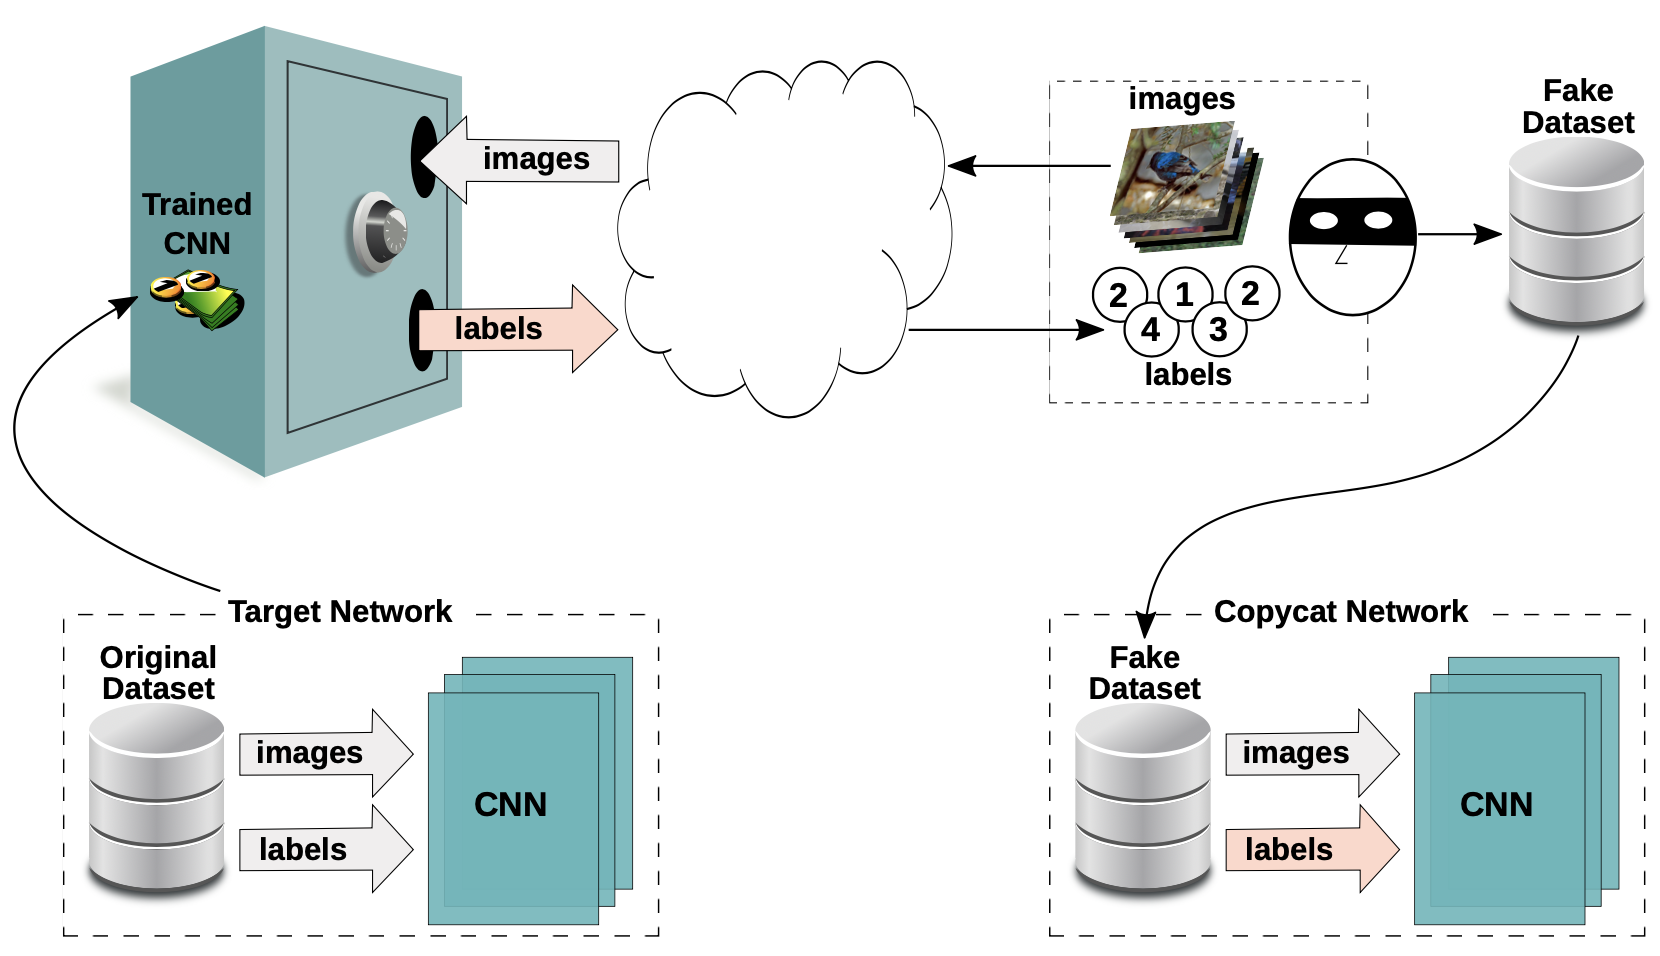
\includegraphics[width=0.75\linewidth]{figures/chapter02/copycatCNN.png}
    \caption{Ataque que realiza CopyCat CNN. \\Fuente: CopyCat CNN \cite{Correia_Silva_2018}}
    \label{fig:copycatcnn}
\end{figure}

En el artículo también demostraron que se podía extraer al menos el 93.7\% del rendimiento de los modelos víctima con datos de dominio no problemáticos y al menos el 98.6\% del rendimiento si se usan datos del dominio del problema. Además, se logró extraer el 97.3\% del modelo de \textit{Microsoft Azure Emotion} usando su API.

% endregion subsubsection Extracción

\subsubsection{Inferencia}
% region subsubsection Inferencia
% \paragraph{Inferencia por Atributos}
% \paragraph{Inferencia por Pertenencia}
% \paragraph{Inversión de modelos}
% \paragraph{Reconstrucción}

En el artículo \cite{10.1145/2810103.2813677} se analizan los ataques de inferencia usando árboles de decisión y un conjunto de datos con información médica de unos individuos, estos ataques permiten extraer información sensible o privada sobre los datos de entrenamiento o sobre las instancias (individuos) a partir de un modelo dé \gls{ML}.

En el artículo se menciona los ataques de inversión de modelo, dicho ataque implica que un atacante abusa del acceso al modelo para extraer información sensible, en concreto habla sobre extraer información genómica sensible de pacientes.

Además, también menciona que se puede extraer los valores de confianza revelados junto con las predicciones, es decir, el nivel de confianza de las predicciones, menciona que se puede usar este dato para inferir información sensible sobre los individuos.

En el artículo \cite{choquettechoo2021labelonly} se mencionan los ataques de inferencia de membresía, estos ataques permiten extraer si una instancia se utilizó para entrenar el modelo. Esto es porque explotan la confianza anormal de los modelos cuando se utilizan instancias del entrenamiento en el modelo entrando. Estos ataques no se pueden usar si el atacante solo obtiene información de la etiqueta y no de la medida de confianza.

En el artículo presentan ataques de membresía usando únicamente etiquetas sin los valores de confianza que estudios anteriores si necesitaban. Esto lo logran evaluando las etiquetas predichas por el modelo en función de determinadas perturbaciones de una instancia.

Ciertas defensas contra estos ataques es la ocultación o alteración del nivel de confianza, en el artículo señalan que los ataques de inferencia de membresía por etiqueta anulan las defensas. Uno de los descubrimientos más relevantes de dicha investigación es que las únicas estrategias de defensas que previenen con éxito todos los ataques son los modelos de entrenamiento con privacidad diferencial y regularización ${L_{2}}$.

% endregion subsubsection Inferencia

% ===================================
% ===================================
\subsection{Defensas en \textit{deep learning}}
\label{sec:defense}
% region subsection Defensas contra los ataques

Se han hecho grandes avances en el estudio de los modelos de inteligencia artificial, se han investigado los posibles ataques y también como defender los modelos frente a alteraciones externas o alteraciones internas.

En las siguientes subsecciones reduciremos la explicación a los artículos más relevantes que se pueden aprovechar en este proyecto.

\subsubsection{Pre procesamiento}
% region subsubsection Pre procesamiento

Estas son algunas de las técnicas de defensa que se pueden aplicar a los modelos antes de su inserción o inferencia.


En el artículo \cite{lin2019invertdefendmodelbasedapproximate} se presenta la técnica \textit{InverseGAN}, con el objetivo de resolver el problema de inferencia en redes \gls{GAN}, creando una red de codificación, aunque no consiguen en la práctica la inversión del código latente si lo logran en un estudio teórico, además demuestran que \textit{InverseGAN} supera a otros métodos de defensa.

En el artículo \textit{DefenseGAN} \cite{samangouei2018defenseganprotectingclassifiersadversarial} se presenta una técnica para defender a los modelos de clasificación, en esta técnica se modela una distribución de imágenes sin perturbaciones y en la inferencia encuentran una versión cercana de la imagen sin cambios adversariales, esta imagen es la que se introduce en el clasificador.

Como los métodos anteriores existen muchos más, aquí se presenta una tabla con los artículos.

% \begin{table}[H]
%     \centering
%     \begin{tblr}{hlines,vlines,rows={valign=m},row{1}={c},colspec={Q[m]X}} 
%         \textbf{Técnica}                & \textbf{Referencias}                                                                                                     \\
%         InverseGAN                      & \href{https://arxiv.org/abs/1911.10291}{An Lin et al., 2019}                                                             \\
%         DefenseGAN                      & \href{https://arxiv.org/abs/1805.06605}{Samangouei et al., 2018}                                                         \\
%         Video Compression               & \href{https://arxiv.org/abs/1902.06705}{Carlini et al., 2019}                                                            \\
%         Resampling                      & \href{https://arxiv.org/abs/1809.10875}{Yang et al., 2019}                                                               \\
%         Thermometer Encoding            & \href{https://openreview.net/forum?id=S18Su--CW}{Buckman et al., 2018}                                                   \\
%         MP3 Compression                 & \href{https://arxiv.org/abs/1801.01944}{Carlini, N. and Wagner, D., 2018}                                                \\
%         Total Variance Minimization     & \href{https://openreview.net/forum?id=SyJ7ClWCb}{Guo et al., 2018}                                                       \\
%         PixelDefend                     & \href{https://arxiv.org/abs/1710.10766}{Song et al., 2017}                                                               \\
%         Gaussian Data Augmentation      & \href{https://arxiv.org/abs/1707.06728}{Zantedeschi et al., 2017}                                                        \\
%         Feature Squeezing               & \href{http://arxiv.org/abs/1704.01155}{Xu et al., 2017}                                                                  \\
%         Spatial Smoothing               & \href{http://arxiv.org/abs/1704.01155}{Xu et al., 2017}                                                                  \\
%         JPEG Compression                & \href{https://arxiv.org/abs/1608.00853}{Dziugaite et al., 2016}                                                          \\
%         Label Smoothing                 & \href{https://pdfs.semanticscholar.org/b5ec/486044c6218dd41b17d8bba502b32a12b91a.pdf}{Warde-Farley and Goodfellow, 2016} \\
%         Virtual Adversarial Training    & \href{https://arxiv.org/abs/1507.00677}{Miyato et al., 2015}                                                             \\
%         Cutout                          & \href{https://arxiv.org/abs/1708.04552}{DeVries et al., 2017}                                                            \\
%         Mixup                           & \href{https://arxiv.org/abs/1710.09412}{Zhang et al., 2017}                                                              \\
%         CutMix                          & \href{https://arxiv.org/abs/1905.04899}{Yun et al., 2019}                                                                \\
%     \end{tblr}
%     \caption{Lista de técnicas de defensa en Deep Learning}
% \end{table}

\begin{longtblr}
    [caption={Lista de técnicas de defensa durante el pre procesamiento en Deep Learning}, label={tab:defense-pre-process}]
    {hlines, vlines, row{1}={c}, rows={valign=m},  colspec={XX}}
    \textbf{Técnica}                & \textbf{Referencias}                                                                                                     \\
    InverseGAN                      & \href{https://arxiv.org/abs/1911.10291}{An Lin et al., 2019}                                                             \\
    DefenseGAN                      & \href{https://arxiv.org/abs/1805.06605}{Samangouei et al., 2018}                                                         \\
    Video Compression               & \href{https://arxiv.org/abs/1902.06705}{Carlini et al., 2019}                                                            \\
    Resampling                      & \href{https://arxiv.org/abs/1809.10875}{Yang et al., 2019}                                                               \\
    Thermometer Encoding            & \href{https://openreview.net/forum?id=S18Su--CW}{Buckman et al., 2018}                                                   \\
    MP3 Compression                 & \href{https://arxiv.org/abs/1801.01944}{Carlini, N. and Wagner, D., 2018}                                                \\
    Total Variance Minimization     & \href{https://openreview.net/forum?id=SyJ7ClWCb}{Guo et al., 2018}                                                       \\
    PixelDefend                     & \href{https://arxiv.org/abs/1710.10766}{Song et al., 2017}                                                               \\
    Gaussian Data Augmentation      & \href{https://arxiv.org/abs/1707.06728}{Zantedeschi et al., 2017}                                                        \\
    Feature Squeezing               & \href{http://arxiv.org/abs/1704.01155}{Xu et al., 2017}                                                                  \\
    Spatial Smoothing               & \href{http://arxiv.org/abs/1704.01155}{Xu et al., 2017}                                                                  \\
    JPEG Compression                & \href{https://arxiv.org/abs/1608.00853}{Dziugaite et al., 2016}                                                          \\
    Label Smoothing                 & \href{https://pdfs.semanticscholar.org/b5ec/486044c6218dd41b17d8bba502b32a12b91a.pdf}{Warde-Farley and Goodfellow, 2016} \\
    Virtual Adversarial Training    & \href{https://arxiv.org/abs/1507.00677}{Miyato et al., 2015}                                                             \\
    Cutout                          & \href{https://arxiv.org/abs/1708.04552}{DeVries et al., 2017}                                                            \\
    Mixup                           & \href{https://arxiv.org/abs/1710.09412}{Zhang et al., 2017}                                                              \\
    CutMix                          & \href{https://arxiv.org/abs/1905.04899}{Yun et al., 2019}                                                                \\
\end{longtblr}

% endregion subsubsection Pre procesamiento
\subsubsection{Post procesamiento}
% region subsubsection Post procesamiento

Las técnicas post procesamiento se implementan después de que el modelo ha realizado su predicción y están diseñadas para mejorar la robustez frente a ataques adversariales.

En estos artículos se plantean defensas frente a extracción de datos, en \textit{Random Noise} \cite{chandrasekaran2019exploringconnectionsactivelearning} se propone un método híbrido para la defensa que combina técnicas clásicas, limitar consultas, monitoreo de patrones de uso, etc. A otros más específicos, como introducir ruido en las respuestas o reducir los modelos para disminuir los datos sensibles que se pueden extraer, también recomiendan técnicas como \textit{data-dependent randomization}.

\begin{table}[H]
    \centering
    \begin{tblr}{hlines, vlines, row{1}={c}, rows={valign=m}, colspec={XX}}
        \textbf{Técnica}    & \textbf{Referencias}                                                  \\
        Reverse Sigmoid     & \href{https://arxiv.org/abs/1806.00054}{Lee et al., 2018}             \\ 
        Random Noise        & \href{https://arxiv.org/abs/1811.02054}{Chandrasekaran et al., 2018}  \\ 
        Class Labels        & \href{https://arxiv.org/abs/1609.02943}{Tramer et al., 2016}, \href{https://arxiv.org/abs/1811.02054}{Chandrasekaran et al., 2018} \\
        High Confidence     & \href{https://arxiv.org/abs/1609.02943}{Tramer et al., 2016}          \\ 
        Rounding            & \href{https://arxiv.org/abs/1609.02943}{Tramer et al., 2016}          \\ 
    \end{tblr}
    \caption{Lista de técnicas de defensa durante el post procesamiento en Deep Learning}
    \label{tab:defense-post-process}
\end{table}

% endregion subsubsection Post procesamiento
\subsubsection{Entrenamiento}

En el proceso de entrenamiento es donde se realizan las técnicas más curiosas y variadas para defender a los modelos.

El artículo \cite{mirman18b} presenta un método para certificar robustez en grandes redes neuronales, dentro de ciertos límites. Este método utiliza varias transformaciones para abstraer la información, equilibrando eficiencia y precisión.

\begin{table}[H]
    \centering
    \begin{tblr}{hlines, vlines, row{1}={c}, rows={valign=m}, colspec={XX}}
        \textbf{Técnica}                & \textbf{Referencias}                                                                                  \\
        General Adversarial Training    & \href{http://arxiv.org/abs/1312.6199}{Szegedy et al., 2013}                                           \\
        Madry's Protocol                & \href{https://arxiv.org/abs/1706.06083}{Madry et al., 2017}                                           \\
        Fast Is Better Than Free        & \href{https://arxiv.org/abs/2001.03994}{Wong et al., 2020}                                            \\
        Certified Adversarial Training  & \href{http://proceedings.mlr.press/v80/mirman18b/mirman18b.pdf}{Mirman et al., 2018} \cite{mirman18b} \\
        Interval Bound Propagation      & \href{https://arxiv.org/abs/1810.12715}{Gowal et al., 2018}                                           \\
        DP-InstaHide                    & \href{https://arxiv.org/abs/2103.02079}{Borgnia et al., 2021}                                         \\
    \end{tblr}
    \caption{Lista completa de técnicas de defensa durante el entrenamiento en Deep Learning}
    \label{tab:defense-train}
\end{table}

% \subsubsection{Transformación}
% \paragraph{Evasión}
% \paragraph{Envenenamiento}
% \subsubsection{Detector}
% \paragraph{Evasión}
% \paragraph{Envenenamiento}

% endregion subsection Defensas contra los ataques

\subsection{Métricas en \textit{deep learning}}
% region subsection Métricas en los ataques adversariales
% DEFINICIÓN DE MÉTRICAS explica que es la {L}_{2}  y {L}_{\infty}

Existen múltiples métricas para evaluar las redes \acrshort{ANN}, entre ellas destacan \textit{Classification Accuracy}, \textit{Logarithmic Loss}, \textit{Confusion Matrix}, etc. Existen también las métricas para validar la seguridad de los modelos, estas son las que nos interesan a nosotros, métricas de robustez, certificación y verificación.


\subsubsection{Robustez}

En el artículo \cite{weng2018evaluating} se analiza el estado de las métricas de robustez y su poca aparición en publicaciones, es por ello que plantean un nuevo enfoque usando la estimación de la constante local de \nameref{theorem::lipschitz} para un análisis de robustez, proponen el uso de la Teoría de Valores Extremos para una evaluación eficiente. Los investigadores la han definido como \gls{CLEVER} independiente de los ataques y computacionalmente eficiente para redes neuronales grandes, dando buenos resultados como las pruebas de robustez indicada por las normas ${\ell_{2}}$ e ${\ell_{\infty}}$. Se considera \gls{CLEVER} como la primera métrica de robustez independiente de ataques aplicable a cualquier red neuronal clasificadora.

\subsubsection{Certificación}

\textit{Randomized Smoothing}  \cite{cohen2019certified} es la técnica que se describe en el artículo de 2019, se usa para mejorar la robustez de un clasificador, esta técnica analiza las perturbaciones adversas, en concreto en la norma ${\ell_{2}}$, demostrando una garantía estricta de robustez en norma ${\ell_{2}}$, esto significa que el clasificador seguirá funcionando correctamente incluso si se introducen perturbaciones en los datos de entrada dentro de unos límites. Los investigadores destacan resultados usando modelos de \gls{ImageNet} con una precisión certificada del ${49\%}$.

\subsubsection{Verificación}

En el artículo \cite{chen2019robustness} de 2019 se aborda la verificación de la robustez en modelos basados en árboles, árboles de decisión, bosques aleatorios, \gls{GBDT}. Proponen un algoritmo de múltiples niveles, algoritmo eficiente que proporciona límites estrictos y permite mejoras iterativas, este algoritmo mejora de forma significativa la velocidad frente a enfoques previos basados en programación lineal.


% endregion subsection Métricas en los ataques adversariales

\subsection{Redes neuronales en \textit{Red team} y \textit{Blue team}}
% region subsection Redes neuronales en Red team y Blue team

Un buen símil entre la seguridad informática clásica y la seguridad en redes neuronales son los conceptos de equipos de ataque y defensa (``\textit{red team}'' y ``\textit{blue team}'').

\begin{figure}[H]
    \centering
    \centerline{\includesvg[width=1\columnwidth]{figures/chapter02/ART-for-red-and-blue-teams.drawio.svg}}
    \caption{Ataques y defensas en redes neuronales.\newline{}Fuente: Elaboración propia.}
    \label{fig:art-for-red-and-blue-teams}
\end{figure}

La idea detrás del aprendizaje automático es la de poder predecir modelos predictivos, para ello se usan conjuntos de datos para el entrenamiento.

Los conjuntos de datos se han de procesar, ya que suelen contener mucho ruido, es decir, información muy poco valiosa, errónea o, por el contrario, una alta dimensionalidad de los datos que puede ser contraproducente por no poder reproducir esas medidas o por la poca información que aportan.

Los ataques al aprendizaje automático o profundo suelen estar dirigidos a las distintas etapas de creación y uso de un modelo.

\begin{itemize}
    \item Alteración de los datos de entrada.
    \item Alteración del proceso de aprendizaje.
    \item Extracción de los datos de entrenamiento.
    \item Bloqueo del modelo.
\end{itemize}

Durante el transcurso del trabajo discutiremos los siguientes ataques y defensas de la sección \nameref{ch:2:section:state-of-the-art:computer-security-in-neural-networks} que se pueden ser vulnerables en los modelos. 

\begin{itemize}
    \item Envenenamiento de datos.
    \item Puerta trasera.
    \item Extracción de datos
    \item Ingeniería inversa.
    \item Evasión.
\end{itemize}

Podemos clasificar las amenazas de la seguridad informática con los siguientes sistemas, \gls{STRIDE}\footnote{Modelado de amenazas de \href{https://learn.microsoft.com/es-es/azure/security/develop/threat-modeling-tool-threats}{microsoft}}, con la matriz \gls{MITRE} o \gls{MITRE-ATLAS}.

\begin{table}[H]
    \centering
    \begin{tblr}{vlines, hlines, rows={valign=m}, colspec={lll}} 
        Spoofing                & Tampering         & Repudiation               \\
        Information disclosure  & Denial of service & Elevation of privilege    \\
    \end{tblr}
    \caption{Modelo para identificar amenazas a la seguridad informática}
    \label{tab:stride}
\end{table}

% \begin{multicols}{2}
%     \begin{itemize}
%         \item Spoofing
%         \item Tampering
%         \item Repudiation
%         \item Denial of service
%         \item Information disclosure
%         \item Elevation of privilege
%     \end{itemize}
% \end{multicols}

\begin{table}[H]
    \centering
    \begin{tblr}{vlines, hlines, rows={valign=m}, colspec={llll}} 
        Reconnaissance      & Resource Development & Initial Access     & Execution  \\ 
        Persistence         & Privilege Escalation & Defense Evasion    & Collection \\ 
        Discovery           & Lateral Movement     & Credential Access  & Impact     \\ 
        Exfiltration        & Command and Control  &                    &            \\ 
    \end{tblr}
    \caption{Clasificación de Amenazas según el Marco MITRE - ATT \& CK}
    \label{tab:mitre}
\end{table}

% \begin{multicols}{3}
%     \begin{itemize}
%         \item Reconnaissance      
%         \item Resource Development 
%         \item Initial Access     
%         \item Execution 
%         \item Persistence         
%         \item Privilege Escalation 
%         \item Defense Evasion    
%         \item Collection 
%         \item Discovery           
%         \item Lateral Movement
%         \item Credential Access
%         \item Impact      
%         \item Exfiltration        
%         \item Command and Control  
%     \end{itemize}
% \end{multicols}

Como hemos visto previamente en las tablas \ref{tab:stride} y \ref{tab:mitre} las amenazas son ataques clásicos que pueden sufrir los sistemas informáticos, mientras que en la tabla \ref{tab:mitre-atlas} se modifican las amenazas de sistemas informáticos que implementen modelos de \acrshort{IA}

\begin{table}[H]
    \centering
    \small
    \begin{tblr}{vlines, hlines, rows={valign=m}, colspec={llll}} 
        Reconnaissance      & Resource Development & Initial Access         & \textbf{ML Model Access}      \\ 
        Execution           & Persistence          & Privilege Escalation   & Defense Evasion               \\ 
        Credential Access   & Discovery            & Collection             & \textbf{ML Attack Staging}    \\ 
        Exfiltration        & Impact               &                        &                               \\ 
    \end{tblr}
    \caption{Clasificación de Amenazas según el Marco MITRE - ATLAS}
    \label{tab:mitre-atlas}
\end{table}

% \begin{multicols}{3}
%      \begin{itemize}
%         \item Reconnaissance      
%         \item Resource Development 
%         \item Initial Access       
%         \item \textbf{ML Model Access}      
%         \item Execution           
%         \item Persistence          
%         \item Privilege Escalation 
%         \item Defense Evasion               
%         \item Credential Access   
%         \item Discovery            
%         \item Collection
%         \item \textbf{ML Attack Staging}    
%         \item Exfiltration        
%         \item Impact
%      \end{itemize}
% \end{multicols}
               

\begin{figure}[H]
    \centering
    \centerline{\includesvg[width=1\linewidth]{figures/chapter02/STRIDE-MITRE-ATLAS.drawio.svg}}
    \caption{Amenazas MITRE - ATT \& CK, MITRE - ATLAS y STRIDE.\newline{}Fuente: Elaboración propia. Inspirado en \href{https://atlas.mitre.org/matrices/ATLAS}{MITRE - ATLAS}}
    \label{fig:amenazas-MITRE-ATLAS-STRIDE}
\end{figure}

% endregion subsection Redes neuronales en Red team y Blue team

\section{Normativa y estándares}

\subsection{El Reglamento Europeo de Inteligencia Artificial}

A partir de 2022 se creó el primer reglamento a nivel Europeo del uso de la Inteligencia artificial. El reglamento establece una jerarquía de riesgos en función del uso de la \acrshort{IA} y sobre las categorías detectadas se establecen unas obligaciones \citet{El-Reglamento-Europeo-de-IA-en-resumen}.

Mediante un análisis de riesgos se han clasificado un conjunto de familias de sistemas de \acrshort{IA} que pueden considerarse de alto riesgo respecto a un riesgo a la salud, seguridad o derechos fundamentales.

El reglamento detalla sistemas de identificación biométrica, infraestructuras críticas, selección y promoción de personal, usos en fronteras o usados por las Fuerzas y Cuerpos de Seguridad del Estado o la Administración de Justicia. También se indica que la lista no es fija y puede ser modificada por un acto delegado.

Los productos que ya cuenten con una normativa armonizada por la \acrshort{UE} deberán ser sometidos a una evaluación de conformidad. También se definen una autoridad de supervisión de mercado como autoridades nacionales competentes.

\begin{figure}[H]
    \centering
    \includegraphics[width=1\linewidth]{figures/chapter02/Pirámide Reglamento Europeo.pdf}
    \caption{Reglamento Europeo\newline{}Fuente: Elaboración propia, inspirado en \cite{El-Reglamento-Europeo-de-IA-en-resumen,reglamento-ia-telefonica}}
    \label{fig:piramide-reglamento-europeo}
\end{figure}

El reglamento define el siguiente esquema para la certificación de productos, una autoridad notificante habilita a organismos de evaluación de conformidad para hacer las evaluaciones de conformidad en materia de \acrshort{IA} a productos que quieran comercializar o poner en funcionamiento. Los productos con regulación deben ser sujetos a la supervisión designada.

Para el caso de sistemas de identificación biométrica utilizados por Fuerzas y Cuerpos de Seguridad del Estado, migración y administración de justicia, las autoridades de supervisión serán las encargadas de supervisar las actividades de seguridad, migración y asilo, en su defecto será la agencia de protección de datos. 

El Comité orientará sobre el reglamento, elaborará guías y establecerá las reglas básicas para elaborar \textit{sandboxes}. Los \textit{sandboxes} permitirán desarrollar y probar sistemas de inteligencia artificial en un entorno regulado. Esto facilitará la elaboración de directrices y reglas más precisas y aplicables, asegurando que las innovaciones en inteligencia artificial se desplieguen de manera segura, ética y conforme a la legislación Europea.

\subsubsection{Sistemas de Inteligencia artificial prohibidos}

Se prohíben los siguientes sistemas de la \acrfull{IA}.

\begin{itemize}
    \item Técnicas subliminales que distorsionen el comportamiento de una persona.
    \item Explotación de vulnerabilidades de un grupo específico de personas por su edad, discapacidad o situación social o económica.
    \item Elaboración de perfiles de personas según su comportamiento, creando un ``baremo social'' que pueda resultar en un trato  des proporcionadamente desfavorable.
    \item Identificación biométrica en tiempo real en lugares accesibles al público por parte de las fuerzas y cuerpos de seguridad, exceptuando muchos casos.
\end{itemize}

El reglamento especifica que la lista puede ser modificada por la Comisión.

\subsubsection{Sistemas de Inteligencia artificial de Alto Riesgo (HRAIS)}

Se definen como sistema de alto riesgo los que cumplan alguna de estas tareas.

\begin{itemize}
    \item Los sistemas que ya cuenten con una legislación Europea Armonizada y estén sujetos a evaluación de conformidad.
    \item Sistemas de identificación biométrica.
    \item Gestión de infraestructuras críticas.
    \item Educación y formación profesional.
    \item Selección de personal y gestión de las relaciones laborales.
    \item Gestión del acceso de las personas a servicios esenciales, públicos y privados.
    \item Actividades de fuerzas y cuerpos de seguridad.
    \item Migración, asilo y control de fronteras.
    \item Administración de justicia y procesos democráticos.
\end{itemize}

Los sistemas de alto riesgo deben cumplir con un nivel adecuado de las siguientes exigencias.

\begin{itemize}
    \item Gestión de riesgos.
    \item Gobernanza y gestión de los datos.
    \item Documentación técnica actualizada.
    \item Registros de actividad del sistema.
    \item Información a los usuarios.
    \item Supervisados por una o varias personas.
    \item Precisión, robustez y seguridad informática.
\end{itemize}

\subsubsection{Obligaciones de transparencia de ciertos sistemas de Inteligencia artificial}

Los proveedores de sistemas deben informar a las personas que están interactuando con un sistema de \acrfull{IA}, excepto cuando se usen para la persecución del crimen.

También se deberá informar a las personas de los sistemas \textit{deep fakes} excepto en persecución del crimen, contenidos evidentemente creativos, satíricos o ficticios.

\subsubsection{Medidas de apoyo a la innovación}

Las autoridades nacionales pueden crear \textit{sandboxes} regulatorios para desarrollar, entrenar, probar y validar sistemas de \acrfull{IA} bajo su guía, supervisión y soporte.

\subsubsection{Gobernanza}

El reglamento designa dos entidades para la gobernanza, el Comité Europeo de Inteligencia Artificial y las Autoridades nacionales competentes.

El Comité Europeo de Inteligencia Artificial, con un representante de cada \acrshort{EEMM} y un grupo permanente de interesados. Sus tareas incluyen, recolección de información técnica y de las mejores prácticas, armonización de pruebas de conformidad, cooperación con organizaciones de expertos en servicios digitales, publicar recomendaciones sobre especificaciones, estándares y guías. Aconsejar a la Comisión en líneas maestras para la implantación del reglamento, etc.

La Autoridad nacional competente deberá designar una autoridad notificadora y una autoridad de supervisión, estas deben ser objetivas e imparciales y deben ser dotadas de los recursos adecuados.

\subsubsection{Monitorización post-comercialización, compartición de información y supervisión de mercado}

Los proveedores de sistemas de alto riesgo deben contar con planes de monitorización apropiados a los riesgos detectados. En caso de cualquier incidente, los proveedores deberán informar a las autoridades de supervisión y a otras autoridades encargadas.

Sé informarán a la Comisión sobre las actividades relacionadas con el Reglamento. Los \acrshort{HRAIS} serán supervisados según la normativa correspondiente: los financieros por el supervisor financiero, los sistemas biométricos por fuerzas de seguridad o la agencia de protección de datos, y las instituciones de la Unión por el Supervisor Europeo de Protección de Datos. Los Estados miembros deben coordinar a las autoridades nacionales de supervisión.

Las autoridades de mercado pueden acceder a datos, código y documentación de los \acrshort{HRAIS} para verificar el cumplimiento, otorgar o denegar permisos para pruebas, y suspender pruebas ante incidentes serios.

Las autoridades de mercado evaluarán sistemas que tengan riesgos y exigir correcciones. Se puede prohibir o restringir sistemas no corregidos y exigir medidas para los que presentan algún riesgo elevado. Se crearán centros de pruebas y un banco de expertos en \acrfull{IA} para apoyar y asesorar.

\subsubsection{Códigos de conducta}

Los códigos de conducta deben ser redactados por los Estados miembros y por la comisión, estos fomentarán la aplicación voluntaria de estos códigos a los sistemas que no sean de alto riesgo.

\subsubsection{Confidencialidad y sanciones}

El reglamento define una tabla de sanciones en función de la falta y la entidad agresora, estas sanciones pueden ser modificadas, además de que se pueden aplicar superiores e inferiores, valorando las circunstancias y el proveedor.


% https://eur-lex.europa.eu/resource.html?uri=cellar:e0649735-a372-11eb-9585-01aa75ed71a1.0008.02/DOC_1&format=PDF
% https://eur-lex.europa.eu/resource.html?uri=cellar:e0649735-a372-11eb-9585-01aa75ed71a1.0008.02/DOC_2&format=PDF

% Según la unión europea toda la seguridad es este apartado :ok: 
% (51) La ciberseguridad es fundamental para garantizar que los sistemas de IA resistan a las actuaciones de terceros maliciosos que, aprovechando las vulnerabilidades del sistema, traten de alterar su uso, conducta o funcionamiento o de poner en peligro sus propiedades de seguridad. Los ciberataques contra sistemas de IA pueden dirigirse contra elementos específicos de la IA, como los conjuntos de datos de entrenamiento (p. ej., contaminación de datos) o los modelos entrenados (p. ej., ataques adversarios), o aprovechar las vulnerabilidades de los elementos digitales del sistema de IA o la infraestructura de TIC subyacente. Por lo tanto, para asegurar un nivel de ciberseguridad adecuado a los riesgos, los proveedores de sistemas de IA de alto riesgo deben adoptar medidas adecuadas teniendo también en cuenta, cuando proceda, la infraestructura de TIC subyacente.

% https://www.youtube.com/@felipebravom

% Feb 1990: Generative Adversarial Networks / Curiosity Generative Adversarial Networks (GANs) have become very popular.[MOST] They were first published in 1990 in Munich under the moniker Artificial Curiosity. [AC90-20][GAN1] Two dueling NNs (a probabilistic generator and a predictor) are trying to maximize each other's loss in a minimax game.[AC](Sec. 1) The generator (called the controller) generates probabilistic outputs (using stochastic units[AC90] like in the much later StyleGANs[GAN2]). The predictor (called the world model) sees the outputs of the controller and predicts environmental reactions to them. Using gradient descent, the predictor NN minimizes its error, while the generator NN tries to make outputs that maximize this error: one net's loss is the other net's gain.[AC90] (The world model can also be used for continual online action planning.[AC90][PLAN2-3][PLAN])
% 4 years before a 2014 paper on GANs,[GAN1] my well-known 2010 survey[AC10] summarised the generative adversarial NNs of 1990 as follows: a "neural network as a predictive world modelis used to maximize the controller's intrinsic reward, which is proportional to the model's prediction errors" (which are minimized).
% The 2014 GANs are an instance of this where the trials are very short (like in bandit problems) and the environment simply returns 1 or 0 depending on whether the controller's (or generator's) output is in a given set.[AC20][AC][T22](Sec. XVII)
% Other early adversarial machine learning settings[S59][H90] were very different—they neither involved unsupervised NNs nor were about modeling data nor used gradient descent.
% The 1990 principle has been widely used for exploration in Reinforcement Learning[SIN5][OUD13] [PAT17][BUR18] and for synthesis of realistic images,[GAN1,2] although the latter domain was recently taken over by Rombach et al.'s Latent Diffusion, another method published in Munich,[DIF1] building on Jarzynski's earlier work in physics from the previous millennium[DIF2]  and more recent papers.[DIF3-5]
% In 1991, I published yet another ML method based on two adversarial NNs called Predictability Minimization for creating disentangled representations of partially redundant data, applied to images in 1996.

% endregion subsection Normativa y estándares

\section{Aplicaciones de las redes neuronales en la seguridad informática}
% Estudio de áreas de aplicación de estas redes en seguridad informática.
% Realizar una revisión bibliográfica del campo de los métodos de redes neuronales adversarias empleadas en seguridad informática.

% region subsection Las redes neuronales para la seguridad informática

Como hemos tratado previamente, existen distintas aplicaciones que se le puede dar a las redes neuronales para segurizar el funcionamiento de un sistema o proteger a un usuario frente ataques maliciosos.

En la actualidad existen muchos tipos de ataque informáticos, entre estos destacan malware, phishing, spam, man in the middle, denegación de servicio, inyección SQL, DNS \textit{Tunneling}, \textit{botnets}, o vulnerabilidades \textit{zero-day} \cite{cisco-attacks}, estos son solo una clasificación rápida de todos los tipos de ataques que se pueden sufrir.

La \gls{IA} ofrece numerosas ventajas en la recopilación de información, toma de decisiones y autonomía de sistemas, podemos usar modelos de inteligencia artificial para mejorar la seguridad clásica de los sistemas de información. Esto permite mejorar la eficiencia de los métodos de seguridad empresarial, seguridad ciudadana, etc.

Estos campos han impulsado una carrera armamentística entre defensores y atacantes, además del desarrollo de códigos éticos y regulaciones internacionales en el ámbito militar.

Algunas herramientas que han llegado al ámbito empresarial para mejorar sus sistemas de seguridad, destacan:

\href{https://cylance.com/}{Cylance} Es una de las principales empresas que proporcionan herramientas de seguridad informática que emplean inteligencia artificial.
\begin{itemize}
    \item CylancePROTECT: plataforma de protección de puntos finales, especializada en identificar y neutralizar malware. Mediante el análisis de archivos y la ejecución de modelos predictivos. Es versátil ya que emplea los modelos predictivos para anticipar el comportamiento de malware desconocido.
    \item CylanceOPTICS: herramienta de detección y respuesta, permite la visualización de las etapas de un ataque, facilita la respuesta rápida y automatizadas basadas en reglas a las amenazas identificando, minimiza el impacto sin bloquear el resto de sistemas no comprometidos.
\end{itemize}

\href{https://www.fortinet.com/lat/products/fortiaiops}{Fortinet} Es una de las empresas con más recorrido en la seguridad informática, especializada en operaciones TI. Cuenta con \texttt{FortiAI}, que es un dispositivo hardware y software para empresas, este cuenta con millones de funciones de malware entrenadas, detecta y analiza amenazas en tiempo real, además de manejar un gran volumen de tráfico de red en tiempo real. Estas soluciones todo en uno vienen acompañadas con decenas de soluciones adicionales. Asume tareas de \gls{IDS}, \gls{SIEM} y \gls{SOAR}.



% endregion subsection Las redes neuronales para la seguridad informática

% TODO: aplicaciones reales de ciberseguridad que usan inteligencia artificial 
{
\Huge
\color{red} 
TODO: 
}
% añadir lista de posibles tareas que pueden realizar las redes neuronales por la seguridad y ejemplos de aplicaciones en producción.

\clearpage\thispagestyle{empty}\cleardoublepage

\chapter{OBJETIVOS}


\section{Analisis}

\section{Ataques}

\section{Defensas}
\clearpage\thispagestyle{empty}\cleardoublepage

\chapter{MATERIALES Y MÉTODOS}

\section{Equipos para la experimentación}

Para el desarrollo de este proyecto se han usado distintos equipos, principalmente un ordenador para el desarrollo y un servidor para el entrenamiento.

Estos son los componentes empleados en el desarrollo del proyecto.

\begin{table}[H]
    \begin{tblr}{rows={valign=m},colspec={p{2.5cm}|l}} 
        CPU         & AMD Ryzen 9 7900X3D 4.4GHz/5.6GHz \\
        RAM         & \makecell[l]{2 x (Corsair Vengeance DDR5 6000MHz 32GB  \\ \hspace{0.8cm}16GB CL30 Memoria Dual AMD EXPO e Intel XMP)} \\
        GPU         & Gigabyte GeForce RTX 4060 EAGLE OC 8GB GDDR6 DLSS3 \\
        Disco duro  & Samsung 990 PRO 2TB SSD PCIe 4.0 NVMe M.2         \\
        Placa base  & MSI MAG X670E TOMAHAWK WIFI
    \end{tblr}
    \caption{Hardware del equipo de desarrollo} 
    \label{tab:hw-my-pc}
\end{table}

\begin{table}[H]
    \begin{tblr}{rows={valign=m},colspec={p{2.5cm}|l}} 
        Producto    & RS720-E9-RS8-G                                    \\
        CPU         & 2 x (Intel(R) Xeon(R) Silver 4210R CPU @ 2.40GHz) \\
        RAM         & 4 x (Samsung M393A8G40AB2-CVF DDR4-2933 64GB)     \\
        GPU         & NVIDIA GA100 [A100 PCIe 80GB]                     \\
        Disco duro  & NVMe SSD 980 PRO 
    \end{tblr}
    \caption{Hardware del equipo de entrenamiento}
    \label{tab:hw-rg2}
\end{table}
% Extracción de caracteristicas clásicas
\section{Extracción y coincidencia de características}
% https://medium.com/@deepanshut041/introduction-to-feature-detection-and-matching-65e27179885d
% https://medium.com/@deepanshut041/introduction-to-sift-scale-invariant-feature-transform-65d7f3a72d40

El objetivo de extracción y coincidencia es el de descubrir una o varias características en dos instancias que permitan reconocer e identificar de forma inequívoca, existe multitud de métodos en \acrfull{CV} para detectar puntos de interés. En esta sección discutiremos los métodos y herramientas que podemos emplear usando de ejemplo las librerías de OpenCV y Scikit-Image.

Existen cientos de aplicaciones en la sociedad y en el mundo industrial, médico, automovilístico, militar, etc. Se incluyen tareas de reconstrucción de imágenes, imágenes 3D, mapeo, estabilización de vídeo, etc. 

Uno de los grandes retos es automatizar robots para que reconozcan y puedan interactuar con el entorno. Para ello se debe reconstruir en 3D el entorno para determinar distancias entre objetos, este es uno de los problemas más difíciles, ya que se deben tener en cuenta puntos de vista, iluminación, oclusión, características de los sensores, etc. Por esta razón, estos métodos deben ser robustos ante problemas de oclusión, rotación, escala, iluminación, deformación, etc. \cite{A-survey-of-feature-matching-methods}

En estudios similares se hace mención de los distintos vectores de ataque que pueden sufrir estos sistemas biométricos, en la denominada ``cadena de suministro''. \cite{Debiasi20b} como podemos observar en la Figura \ref{fig:attack-vectors}.

\begin{figure}[H]
    \centering
    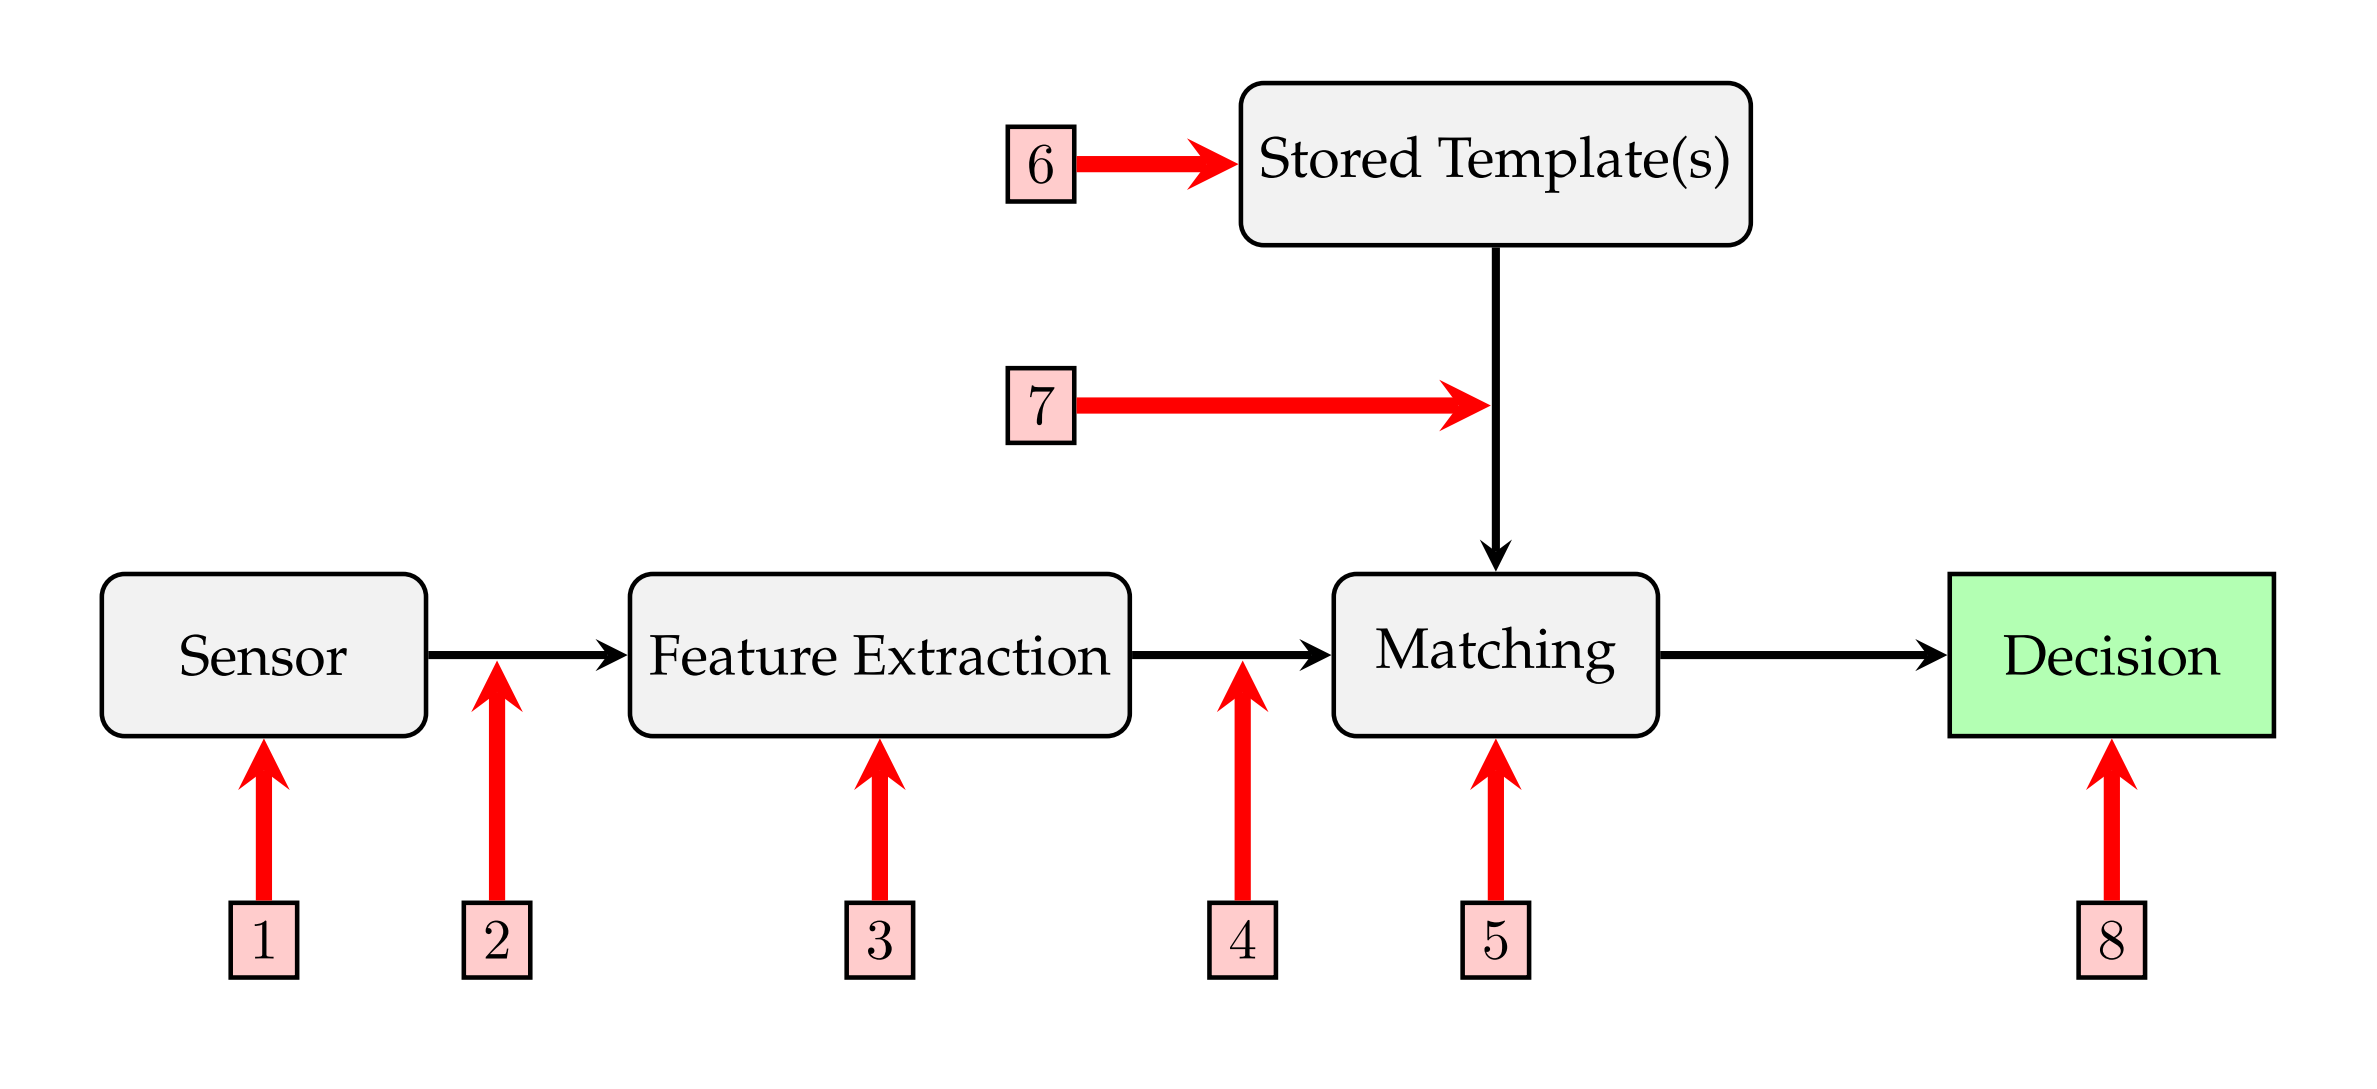
\includegraphics[width=0.8\linewidth]{figures/chapter04/Attack vectors in a generic biometric system.png}
    \caption{Attack vectors in a generic biometric system\newline{}Fuente: Exploiting Image Sensor Data in Biometric Systems and Mobile Applications \cite{Debiasi20b}}
    \label{fig:attack-vectors}
\end{figure}

Actualmente, se clasifican los algoritmos en métodos basados en \textbf{regiones} o métodos basados en \textbf{características}. En los métodos por regiones usan la comparación directa, estos emplean una ventana deslizante que comparará ambas regiones. Los métodos basados en características ofrecen más flexibilidad y estabilidad, estos métodos busca detectar estructuras (esquinas, bordes, formas), con el objetivo de generar descriptores robustos. Se debe tomar las muestras validando de que sean útiles, que no haya un sobre muestreo. Estos métodos dan buenos resultados, pero a costa de un coste computacional muy elevado cuando la resolución de imágenes o vídeos aumenta.

La extracción de características debe ser robusta para su posterior comparación, los métodos por \gls{ANN} usan capas convolucionales, estas capas generarán descriptores basados en las coordenadas de las características y sus relaciones de vecindad. También existen los extractores \textit{end-to-end} que permiten generar los descriptores directamente desde imágenes.

\begin{figure}[H]
    \centering
    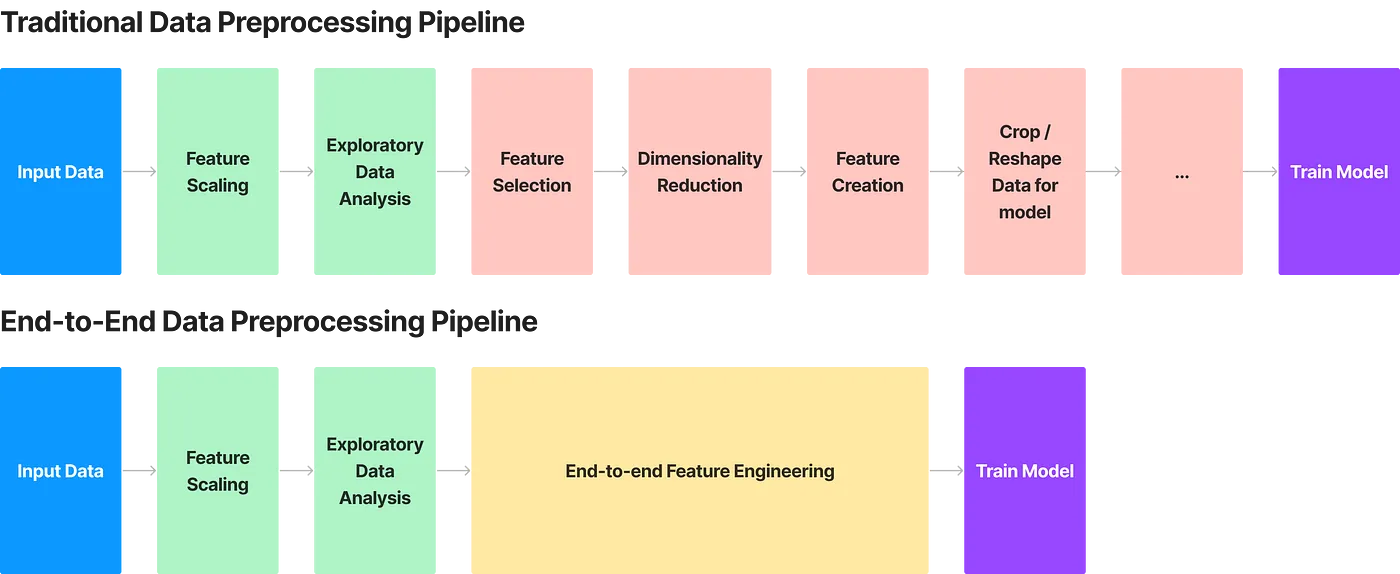
\includegraphics[width=0.5\linewidth]{figures/chapter02/end-to-end.png}
    \caption{End to end feature engineering methods \\Fuente: \href{https://ryendu.medium.com/end-to-end-transformational-feature-engineering-with-cnns-52a5125a10}{End-to-end transformational Feature Engineering with CNNs}}
    \label{fig:end-to-end-cnn}
\end{figure}

\begin{figure}[H]
    \centering
    % 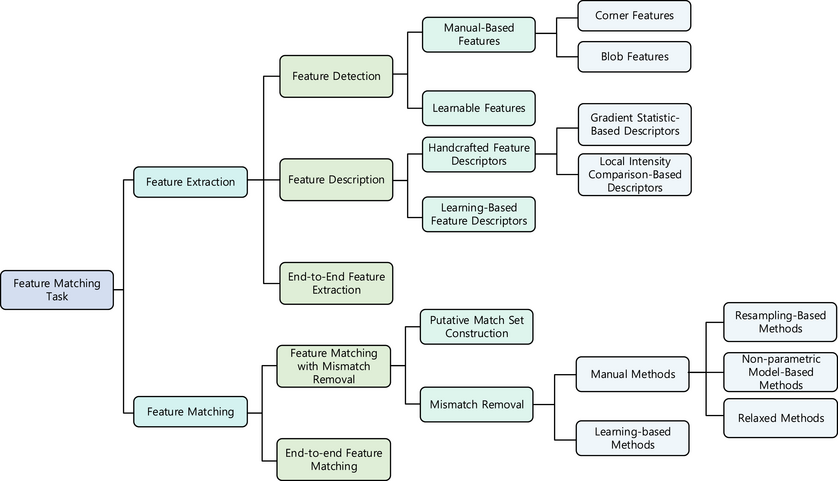
\includegraphics[width=0.5\linewidth]{figures/chapter04/Classification-of-feature-matching-methods.png}
    \centerline{\includesvg[width=1\linewidth]{figures/chapter04/Classification-of-feature-matching-methods.drawio.svg}}
    \caption{Clasificación de métodos de extracción y coincidencia de características. \\Fuente: A survey of feature matching methods \cite{A-survey-of-feature-matching-methods}}
    \label{fig:classification-of-feature-matching-methods}
\end{figure}

Como podemos ver en la Figura \ref{fig:classification-of-feature-matching-methods} existen una gran variedad de métodos y para las distintas tareas dentro de la extracción y coincidencia en \acrfull{CV}, a continuación se listan los algoritmos clásicos más relevantes en la literatura actual. Posteriormente, se identificarán algunos de los métodos de redes neuronales más relevantes en la literatura que permiten también extraer y comparar puntos de interés.

\footnotetext[1]{OpenCV Python cuenta con una implementación experimental.}
\footnotetext[2]{Algoritmo patentado hasta el año 2020}
\footnotetext[3]{Algoritmo patentado hasta el año 2028}


Algunas de las herramientas que permite usar estos algoritmos y métodos son las librerías de \texttt{OpenCV} y \texttt{scikit-image}, estas librerías no implementa todos los métodos que requerimos, pero sí una gran cantidad de ellos.

\begin{figure}[H]
    \centering
    \begin{subfigure}{.25\linewidth}
        \centerline{\includesvg[width=\linewidth]{figures/assets/OpenCV.svg}}
        \caption{Librería OpenCV}
        \label{subfig:opencv}
    \end{subfigure} 
    \hspace{0.10\textwidth} % Espacio horizontal
    \begin{subfigure}{.25\linewidth}
        
\includegraphics[width=\linewidth]{figures/assets/scikit-image.png}
        \caption{Librería scikit-image}
        \label{subfig:scikit-image}
    \end{subfigure}

    \caption{Librerías para el tratamiento de imágenes}
    \label{fig:libs-images}
\end{figure}


% Distancia Euclidiana: Para descriptores flotantes (SIFT, SURF, etc.).
% Distancia de Hamming: Para descriptores binarios (ORB, BRIEF, BRISK).

% https://riunet.upv.es/bitstream/handle/10251/123298/Agust%C3%AD%20-%20Introducci%C3%B3n%20a%20la%20detecci%C3%B3n%20de%20puntos%20caracter%C3%ADsticos%20con%20OpenCV.pdf?sequence=1
% EL SDK de OpenCV ofrece varios algoritmos para la detección de puntos característicos [7] como AGAST, GFTTDetector, FastFEatureDetector, ORB, AKAZE, BRISK, KAZE o MSER. También existen otros que OpenCV los divide en dos grupos un tanto especiales: experimentales (BoostDesc, BRIEF, DAISY, FREAK, LATCH, LUCID, MSDDetector, PCTSignaturesSQFD, StarDetector o VGG) y extra (compuesto por SIFT, SURF y una versión de SURF optimizada para CUDA,

% Alternativas a SIFT o SURF pueden ser BRISK o FREAK

Explicaremos algunos de los métodos más relevantes y usados en \gls{CV} para la detección de puntos de referencia y sus descriptores. Estos métodos permiten identificar de forma eficiente distintas huellas o identificadores biométricos.

\subsection{Algoritmos de detección de puntos de interés}

\begin{itemize}
    \item \textbf{Bordes}:      % (Operador Roberts cross (1965) \cite{roberts1965machine,angenent2006mathematical}, Robinson (1977) \cite{robinson1977edge}, Canny (1986) \cite{canny1986computational}, Deriche (1987) \cite{deriche1987using}, Differential (1998) \cite{lindeberg1998edge}, STAR Detector (2008) \cite{agrawal2008censure}, Operador Prewitt (2013) \cite{dim2013alternative}, Operador Sobel (2014) \cite{sobelIrwin2014})
    \begin{itemize}
        \item Operador Roberts cross (1965) \cite{roberts1965machine,angenent2006mathematical}
        \item Robinson (1977) \cite{robinson1977edge}
        \item Canny (1986) \cite{canny1986computational}
        \item Deriche (1987) \cite{deriche1987using}
        \item Differential (1998) \cite{lindeberg1998edge}
        \item STAR Detector (2008) \cite{agrawal2008censure}
        \item Operador Prewitt (2013) \cite{dim2013alternative}
        \item Operador Sobel (2014) \cite{sobelIrwin2014}
    \end{itemize}

    \item \textbf{Esquinas}:    % (Harris operator (1988) \cite{Harris88alvey}, Shi-Tomasi (1994) \cite{Shi-and-Tomasi--good-features-to-track}, FAST (1994) \cite{rosten2005fusing,rosten2006machine})
    \begin{itemize}
        \item Harris operator (1988) \cite{Harris88alvey}
        \item Shi-Tomasi (1994) \cite{Shi-and-Tomasi--good-features-to-track}
        \item FAST (1994) \cite{rosten2005fusing,rosten2006machine}
    \end{itemize}
    
    \item \textbf{Blobs}:       % (SIFT\footnotemark[2] (1999) \cite{sift}, AKAZE (2011) \cite{akaze-alcantarilla2011fast})
    \begin{itemize}
        \item SIFT\footnotemark[2] (1999) \cite{sift}
        \item AKAZE (2011) \cite{akaze-alcantarilla2011fast}
    \end{itemize}
    
    \item \textbf{Crestas}:     % (Hough transform (1972) \cite{duda1972use})
    \begin{itemize}
        \item Hough transform (1972) \cite{duda1972use}
    \end{itemize}

    \item \textbf{Regiones}:    % (MSER (2006) \cite{donoser2006efficient})
    \begin{itemize}
        \item MSER (2006) \cite{donoser2006efficient}
    \end{itemize}
\end{itemize}


\subsection{Algoritmos de cálculo de descriptores de puntos de interés}
\begin{itemize}
    \item \textbf{Orientación de gradientes}: 
    \begin{itemize}
        \item SIFT\footnotemark[2] (1999) \cite{sift}
        \item HOG (2005) \cite{dalal2005histograms}
        \item GLOH (2005) \cite{mikolajczyk2005performance}
        \item SURF\footnotemark[3] (2006) \cite{bay2006surf,BAY2008346}
        \item CSIFT (2006) \cite{abdel2006csift}
        \item DAISY\footnotemark[1] (2009) \cite{tola2009daisy}
        \item RootSIFT (2012) \cite{arandjelovic2012three}
    \end{itemize}
    
    \item \textbf{Binarios}: 
    \begin{itemize}
        \item BRIEF\footnotemark[1] (2010) \cite{calonder2010brief}
        \item AKAZE (2011) \cite{akaze-alcantarilla2011fast}
        \item BRISK (2011) \cite{leutenegger2011brisk}
        \item ORB (2011) \cite{rublee2011orb}
        \item LATCH (2016) \cite{Riggan20162016IW}
    \end{itemize}
\end{itemize}


\subsection{Algoritmos de búsqueda de descriptores}
\begin{itemize}
    \item \textbf{Búsqueda lineal}: 
    \begin{itemize}
        \item Brute-Force Matcher \cite{bf-and-flann-matcher}
    \end{itemize}
    
    \item \textbf{Búsqueda aproximada}: 
    \begin{itemize}
        \item FLANN (2012) \cite{bf-and-flann-matcher,10.5555/2354409.2355123}
    \end{itemize}
\end{itemize}

En la literatura se mencionan principalmente dos métodos de búsqueda de descriptores, método por fuerza bruta o búsqueda aproximada (FLANN \cite{bf-and-flann-matcher,10.5555/2354409.2355123}).

Estos métodos presentan ventajas y desventajas, la principal ventaja es que son sencillos y muy eficientes, la principal desventaja el coste computacional cuando la extracción ha dado un gran número de puntos de interés. Actualmente, ya existen métodos que solucionan el problema de alta densidad en la coincidencia de descriptores, como es el caso de \acrshort{FDD} \cite{FDD-pan2024fixedlengthdensedescriptorefficient}.

\subsection{Redes neuronales para la detección y coincidencia}
A continuación se explican otros métodos que son relevantes, ya que usan redes neuronales y métodos de inteligencia artificial para extraer y comprobar la coincidencia de instancias biométricas.

Estos son los métodos \textit{end-to-end} mencionados previamente que permite extraer directamente descriptores desde una imagen usando redes neuronales.

\begin{itemize}
    \item \texttt{SuperPoint} \cite{detone18superpoint} es un modelo basado en redes neuronales, este es de los más relevantes en esta tarea que, ya que permite detectar y describir puntos de interés.
    \item \texttt{KeyNet} \cite{Barroso-Laguna2019ICCV} es otro de los modelos que permite detectar puntos de interés robustos mediante filtros \gls{CNN}.
    \item \texttt{D2-Net} \cite{D2-Net-Dusmanu2019CVPR} es uno de los trabajos más recientes, dicha red permite detectar y describir puntos de interés, aunque en este caso ellos invierten el proceso y describen para posteriormente detectar los puntos de interés. Es robusto y fiable en instancias con cambios de iluminación.
\end{itemize}


\subsection{Otros algoritmos o métodos}
\subsubsection{Iterative Closest Point Algorithm (ICP)}
Es un algoritmo iterativo de puntos más cercanos (\acrfull{ICP}), que consiste en transformar iterativamente un conjunto de características para que coincidan mejor con otro, minimizando una métrica de error basada normalmente en una distancia (distancia euclidiana) \cite{Salhi2019}.

Existen algunas implementaciones externas de este algoritmo, en nuestro caso partiremos de esta implementación que usa \texttt{opencv}. \href{https://github.com/abreheret/icp-opencv}{abreheret/icp-opencv}


%%%%%%%%%%%%%%%%%% IMPORTANTE 
% Esta puede ser muy relevante para el trabajo, ya que nos permitiría crear instancias que van iterando 
% Analizar el repo y el articulo https://github.com/JooseRajamaeki/ICP/tree/master
%%%%%%%%%%%%%%%%%% IMPORTANTE 


\subsection*{SIFT (Scale Invariant Feature Transform)}
% https://medium.com/@deepanshut041/introduction-to-sift-scale-invariant-feature-transform-65d7f3a72d40
Es uno de los métodos más relevantes en \acrshort{CV}, este permite detectar puntos característicos en una imagen y luego describirlos mediante un histograma orientado de gradientes. \cite{sift}

El algoritmo cuenta con dos partes, la extracción de puntos de interés y la descripción de la región del punto de interés. La detección de puntos de interés detecta mediante esquinas y mediante \textit{blobs}.

\begin{itemize}
    \item \textbf{Localidad}
    \item \textbf{Distinción}
    \item \textbf{Cantidad}
    \item \textbf{Eficiencia}
    \item \textbf{Extensibilidad}
\end{itemize}

Una de las grandes desventajas de este algoritmo es su velocidad, además estaba patentado hasta el año 2020, lo que hizo que no se pudiera usar en productos comerciales, pero sí en investigación.

% \subsection{SURF (Speeded-Up Robust Features)}

% \subsection{FAST (Features from Accelerated Segment Test)}

% \subsection{BRISK (Binary Robust Invariant Scalable Keypoints)}

% \subsection{BRIEF (Binary Robust Independent Elementary Features)}

% \subsection{ORB (Oriented FAST and Rotated BRIEF)}



% https://www.geeksforgeeks.org/image-processing-in-python/
\section{Análisis de frameworks de Deep Learning}

Encontrar un \textit{framework} que cubra nuestras necesidades es una tarea compleja, ya que hay una gran variedad de estos que aun siendo respaldados sus desarrollos por grandes empresas son abandonados y puede no cumplir con nuestrar

En la siguiente sección sé muestran y se explican las características de los principales \textit{frameworks} de desarrollo de modelos de redes neuronales profundas más relevante del momento.

% =====================================
% ==== KERAS
% =====================================
\subsection{Keras}

\begin{figure}[H]
    \centering
    
\includegraphics[width=7cm]{figures/assets/Logo_Keras.png}
    \caption{Keras}
    \label{fig:lib-keras}
\end{figure}

Keras \cite{chollet2015keras} es uno de los primeros \textit{frameworks} en la creación y ejecución de modelos de redes neuronales profundas, publicada en 2015, bajo la licencia \gls{LICENSE-MIT}, es de código abierto, soporta múltiples entornos de ejecución como \texttt{TensorFlow} \cite{Abadi_TensorFlow_Large-scale_machine_2015} o \texttt{CNTK} \cite{10.1145/2939672.2945397}.

Escrita en \texttt{python} el proyecto está estructurado en módulos independientes que suelen trabajar en conjunto, cuenta con soporte para capas neuronales, funciones de perdida, optimizadores, métricas, etc. Además, también permite extender estos módulos para adaptarlos a tus propias modificaciones. 

El objetivo principal de \texttt{Keras} es el de ser una interfaz intuitiva en vez de un framework completo, ya que utiliza se implementó el núcleo de \texttt{tensorflow}.

Características principales:
\begin{itemize}
    \item Interfaz sencilla para crear redes neuronales
    \item Definida por módulos que permiten agregar funcionalidades.
    \item Sencilla de extender sus características.
\end{itemize}

% \begin{table}[H]
%     \centering
%     \begin{tblr}{hlines,vlines,rows={valign=m},row{1}={c},colspec={XX}} 
%         \textbf{Ventajas}                           & \textbf{Desventajas}                             \\ 
%         Fácil de usar para principiantes            & Menos funciones avanzadas que otros frameworks   \\
%         Rápido de aprender para usuarios expertos   & Más restringido que frameworks avanzados         \\
%         Buena integración con frameworks            &                                                  \\
%     \end{tblr}
%     \caption{Keras: Ventajas y desventajas}
%     \label{tab:tensorflow-pros-cons}
% \end{table}


\begin{minipage}[t]{0.45\textwidth}
    \centering
    \textbf{Ventajas} \\[1ex]
    \begin{itemize}
        \item Fácil de usar para principiantes
        \item Rápido de aprender para usuarios expertos
        \item Es la base de otros frameworks
    \end{itemize}
\end{minipage}%
\hfill
\begin{minipage}[t]{0.45\textwidth}
    \centering
    \textbf{Desventajas} \\[1ex]
    \begin{itemize}
        \item Menos funciones avanzadas que otros frameworks
        \item Más restringido que frameworks avanzados
    \end{itemize}
\end{minipage}

% =====================================
% ==== TENSORFLOW
% =====================================
\subsection{TensorFlow}

\begin{figure}[H]
    \centering
    
\includegraphics[width=7cm]{figures/assets/Logo_TensorFlow.png}
    \caption{TensorFlow}
    \label{fig:lib-tensorflow}
\end{figure}

TensorFlow \cite{Abadi_TensorFlow_Large-scale_machine_2015} es el \textit{framework} del grupo de investigación de inteligencia artificial de Google, es de código abierto y cuenta con la licencia \gls{LICENSE-APACHE-2}. Es uno de los más completos, cuenta con un amplio ecosistema, ya que se enfoca en proyectos empresariales. Proporciona una \gls{API} de \texttt{python} así como para los lenguajes de \texttt{C++}, \texttt{Haskell}, \texttt{Java}, \texttt{Go} y \texttt{Rust}, existen otras implementaciones de terceros de la \gls{API} de \texttt{TensorFlow}.

Además, se expande mediante implementaciones de alto rendimiento para dispositivos de bajos recursos, como es el caso de \texttt{tensorflow.js}, este permite ejecutar modelos ligeros directamente en un navegador web, ofrece distintos \gls{TENSORFLOW-BACKEND}. La \gls{API} es flexible y permite el uso de funciones de \texttt{Keras}.

Características principales:
\begin{itemize}
    \item Soporta un gran conjunto de herramientas y librerías para la construcción de redes neuronales, tanto convolucionales como recurrentes.
    \item Soporte para distintos tipos de hardware, tanto \gls{CPU}, \gls{GPU}, \gls{TPU}
\end{itemize}

% \begin{table}[H]
%     \centering
%     \begin{tblr}{hlines,vlines,rows={valign=m},row{1}={c},colspec={XX}} 
%         \textbf{Ventajas}                 & \textbf{Desventajas}                        \\ 
%         Multiplataforma                   & Curva de aprendizaje alta                   \\
%         Gran soporte a muchas tareas      & Grafo estático poco eficiente ante cambios  \\
%         Soporte y documentación           &                                             \\
%         Compatible con uso industrial     &                                             \\
%     \end{tblr}
%     \captionsetup{justification=centering}
%     \caption{TensorFlow: Ventajas y desventajas}
%     \label{tab:pros_cons}
% \end{table}

\begin{minipage}[t]{0.45\textwidth}
    \centering
    \textbf{Ventajas} \\[1ex]
    \begin{itemize}
        \item Multiplataforma
        \item Gran soporte a muchas tareas
        \item Soporte y documentación
        \item Compatible con uso industrial
    \end{itemize}
\end{minipage}%
\hfill
\begin{minipage}[t]{0.45\textwidth}
    \centering
    \textbf{Desventajas} \\[1ex]
    \begin{itemize}
        \item Curva de aprendizaje alta
        \item Grafo estático poco eficiente ante cambios
    \end{itemize}
\end{minipage}

% =====================================
% ==== PYTORCH
% =====================================
\subsection{PyTorch}

\begin{figure}[H]
    \centering
    
\includegraphics[width=7cm]{figures/assets/Logo_PyTorch.png}
    \caption{PyTorch}
    \label{fig:lib-pytorch}
\end{figure}

PyTorch \cite{Ansel_PyTorch_2_Faster_2024} es uno de los \textit{frameworks} actuales más relevantes para el desarrollo de modelos de inteligencia artificial, es de código abierto y es desarrollada principalmente por \textit{Facebook's AI Research lab} (FAIR), cuenta con una licencia libre \gls{LICENSE-BSD}, fue lanzado en 2016. 

Cuenta con soporte para Windows, Linux y MacOS, cuenta con soporte para gestores de paquetes de \texttt{conda} y \texttt{pip}, además PyTorch distribuye su librería para otros sistemas (C++) mediante \texttt{LibTorch}, da soporte para tarjetas gráficas NVIDIA con tecnología \texttt{CUDA[11.8, 12.1, 12.4]}, tarjetas gráficas \texttt{AMD ROCm[6.2]} o \gls{CPU}.

Sus principales ventajas es que es la fusión de varios proyectos con otras organizaciones, por lo que existe una compatibilidad entre estos \textit{Frameworks}. Es compatible con otras librerías de ciencias de datos, \textit{numpy}, \textit{scipy}, \textit{panda}.

% Características 
Soporta la ejecución y entrenamiento en \gls{GPU} y \gls{TPU} y la distribución entre múltiples tarjetas gráficas, cuenta con una \gls{API} disponible para otros lenguajes, además de modelos pre-entrenados, conjuntos de datos o ejemplos de arquitecturas comunes en la literatura actual.

% Ecosistema
PyTorch cuenta con un gran ecosistema, estos son otros proyectos que expanden la librería y permite realizar, desde visualización de los procesos, entrenamientos o resultados, exportar los modelos a otros entornos de ejecución, etc.

\textbf{Características principales}:
\begin{itemize}
    \item PyTorch trabaja con un grafo dinámico haciendo que el desarrollo y experimentación sea más rápido.
    \item Programación imperativa permite construir modelos más sencillos.
    \item Soporte para \gls{GPU}, \gls{TPU}, etc.
\end{itemize}

% \begin{table}[H]
%     \centering
%     \begin{tblr}{hlines,vlines,rows={valign=m},row{1}={c},colspec={Q[m]X}} 
%         \textbf{Ventajas}                          & \textbf{Desventajas}                       \\ 
%         Fácil para principiantes                   & Menos funciones que TensorFlow             \\
%         Adaptable para desarrollo e investigación  & Menos opciones para despliegue             \\
%         Compatible con grafo dinámico              &                                           \\
%     \end{tblr}
%     \caption{PyTorch: Ventajas y desventajas}
%     \label{tab:pytorch-pros_cons}
% \end{table}

\begin{multicols}{2} % Inicia el entorno de dos columnas
    \centering
    \textbf{Ventajas} \\[1ex]
    \begin{itemize}
        \item Fácil para principiantes
        \item Adaptable para desarrollo e investigación
        \item Compatible con grafo dinámico
    \end{itemize}
    
    \columnbreak % Cambia a la siguiente columna

    \centering
    \textbf{Desventajas} \\[1ex]
    \begin{itemize}
        \item Menos funciones que TensorFlow
        \item Menos opciones para despliegue
    \end{itemize}
\end{multicols}

\begin{table}[H]
    \centering
    \begin{tblr}{hlines,vlines,rows={valign=m},colspec={Q[m]X}} 
        \textbf{Módulo}             & \textbf{Descripción}                                                                      \\ 
        \texttt{torch}              & Biblioteca principal para el cálculo numérico y la manipulación de tensores.              \\ 
        \texttt{torch.nn}           & Proporciona herramientas para construir redes neuronales y capas.                         \\ 
        \texttt{torch.autograd}     & Soporte para la diferenciación automática para la optimización del entrenamiento.         \\ 
        \texttt{torch.optim}        & Optimizadores, como SGD y Adam, para ajustar los parámetros de los modelos.               \\ 
        \texttt{torch.utils.data}   & Herramientas para el manejo de datos y su carga durante el entrenamiento.                 \\
    \end{tblr}
    \caption{Núcleo de PyTorch}
    \label{tab:pytorch-modules}
\end{table}

\begin{table}[H]
    \centering
    \begin{tblr}{hlines,vlines,rows={valign=m},colspec={Q[m]X}} 
        \textbf{Tecnologías}    & \textbf{Descripción}                                                                                      \\ 
        \texttt{torch.cuda}     & Permite el uso de GPUs NVIDIA para acelerar los cálculos de tensores                                      \\
        \texttt{torch.onnx}     & Herramientas para exportar modelos de PyTorch al formato ONNX para interoperabilidad con otros frameworks \\
    \end{tblr}
    \caption{Tecnologías de PyTorch}
    \label{tab:pytorch-gpu}
\end{table}

\begin{table}[H]
    \centering
    \begin{tblr}{hlines,vlines,rows={valign=m},colspec={Q[m]X}} 
        \textbf{Librería}       & \textbf{Descripción}                                                                                  \\ 
        \texttt{torchvision}    & Conjunto de bibliotecas para tareas de visión por computadora, con modelos preentrenados y utilidades \\ 
        \texttt{torchaudio}     & Biblioteca para trabajar con datos de audio, con soporte para diversas operaciones de audio           \\ 
        \texttt{torchtext}      & Biblioteca para la carga, preprocesamiento y uso de datos de texto en tareas de NLP                   \\
    \end{tblr}
    \caption{Librería de PyTorch}
    \label{tab:pytorch-lib}
\end{table}



% =====================================
% ==== PyTorch + PyTorch Lightning
% =====================================
\subsection{PyTorch Lightning}

\begin{figure}[H]
    \centering
    
\includegraphics[width=7cm]{figures/assets/Logo_Lightning.png}
    \caption{PyTorch Lightning}
    \label{fig:pytorch-lightning}
\end{figure}

PyTorch Lightning \cite{Falcon_PyTorch_Lightning_2019} es un framework que expande y simplifica PyTorch, este permite simplificar el código de PyTorch a una arquitectura de objetos con el objetivo de realizar módulos más reutilizables.

Este framework permite simplificar y abstraer el código, controla la gestión de memoria y de dispositivos, permite crear y pruebas o depurar de forma más sencilla. 

Cuenta con una extensa \texttt{API}, cuenta con gestión de modelos en dispositivos \textit{Accelerators}, ejecución de funciones por eventos mediante \texttt{Callbacks}, un \gls{CLI} para la gestión por terminal, gestión de \texttt{logs}, control del entrenamiento mediante la clase \texttt{Trainer}, gestión automática de hiperparámetros mediante \texttt{Tuner} y muchas más utilidades.


\subsection{Otras alternativas, frameworks de deep learning}

Se han analizado muchos frameworks que cumplen parcialmente nuestras necesidades, algunas de las alternativas son las siguientes. Muchos de estos proyectos siguen en desarrollo y aumentando sus capacidades, aunque otros o han llegado a su objetivo o han sido abandonados parcial o totalmente.

\begin{table}[H]
    \centering
    \begin{tblr}{hlines,vlines,rows={valign=m},colspec={XX}} 
        \textbf{Framework}      & \textbf{Especialización}  & \textbf{Empresa}              & \textbf{Estado}   \\ 
        MXNet                   & Generalista               & F. APACHE y Amazon            & En desarrollo     \\ 
        CAFFE                   & Visión por computador     & Berkeley AI Research          & Abandonado        \\ 
        CNTK                    & Generalista               & Microsoft                     & Abandonado        \\ 
        LangChain               & LLMs                      & LangChain, Inc                & En desarrollo     \\ 
        OpenNN                  & Generalista               & Artelnics                     & Abandonado        \\ 
        Deeplearning4j          & Generalista               & Kondiut and contributors      & En desarrollo     \\ 
        Chainer                 & Generalista               & Seiya and contributors        & Abandonado        \\ 
    \end{tblr}
    \caption{Frameworks de deep learning}
    \label{tab:other-frameworks}
\end{table}


\clearpage
\section{Bibliotecas para ciencia de datos}
% https://verneacademy.com/blog/articulos-ia/10-librerias-python-data-science-machine-learning/

Existe una gran variedad de bibliotecas y librerías que ofrecen soluciones a los principales problemas en el campo de la ciencia de datos y de la inteligencia artificial. A continuación mostramos las herramientas más usadas por la comunidad científica y cuáles son sus características.

\begin{figure}[H]
    \centering
    % Primera fila de imágenes
    \captionsetup{justification=centering}
    % \captionsetup[subfigure]{justification=justified}

    \begin{subfigure}{0.15\textwidth}
        \centering
        \includegraphics[width=1\textwidth]{figures/chapter04/lib/Pandas.png}
        \caption{Pandas}
        \label{fig:imagen1}
    \end{subfigure}
    \hfill
    \begin{subfigure}{0.15\textwidth}
        \centering
        \includegraphics[width=1\textwidth]{figures/chapter04/lib/NumPy.png}
        \caption{NumPy}
        \label{fig:imagen2}
    \end{subfigure}
    \hfill
    \begin{subfigure}{0.15\textwidth}
        \centering
        \includegraphics[width=1\textwidth]{figures/chapter04/lib/Plotly.png}
        \caption{Plotly}
        \label{fig:imagen3}
    \end{subfigure}
    
    \bigskip 
    
    % Segunda fila de imágenes
    \begin{subfigure}{0.15\textwidth}
        \centering
        \includegraphics[width=1\textwidth]{figures/chapter04/lib/Matplotlib.png}
        \caption{Matplotlib}
        \label{fig:imagen4}
    \end{subfigure}
    \hfill
    \begin{subfigure}{0.15\textwidth}
        \centering
        \includegraphics[width=1\textwidth]{figures/chapter04/lib/scikit-learn.png}
        \caption{scikit-learn}
        \label{fig:imagen5}
    \end{subfigure}
    \hfill
    \begin{subfigure}{0.15\textwidth}
        \centering
        \includegraphics[width=1\textwidth]{figures/chapter04/lib/shap.png}
        \caption{shap}
        \label{fig:imagen6}
    \end{subfigure}
    
    \caption{Bibliotecas de Python para ciencia de datos}
    \label{fig:cuadricula}
\end{figure}

% \begin{figure}[H]
%     \centering
%     \begin{subfigure}{0.15\textwidth}
%         \centering
%         \includegraphics[width=\textwidth]{figures/chapter04/lib/Pandas.png}
%         \caption{Pandas}
%         \label{fig:imagen1}
%     \end{subfigure}
%     \hspace{0.02\textwidth} % Espacio horizontal
%     \begin{subfigure}{0.15\textwidth}
%        \centering
%         \includegraphics[width=\textwidth]{figures/chapter04/lib/NumPy.png}
%         \caption{NumPy}
%         \label{fig:imagen2}
%     \end{subfigure}
    
%     \hspace{0.10\textwidth} % Espacio horizontal
    
%     \begin{subfigure}{0.15\textwidth}
%         \centering
%         \includegraphics[width=\textwidth]{figures/chapter04/lib/Plotly.png}
%         \caption{Plotly}
%         \label{fig:imagen3}
%     \end{subfigure}
%     \hspace{0.02\textwidth} % Espacio horizontal
%     \begin{subfigure}{0.15\textwidth}
%         \centering
%         \includegraphics[width=\textwidth]{figures/chapter04/lib/Matplotlib.png}
%         \caption{Matplotlib}
%         \label{fig:imagen4}
%     \end{subfigure}

%     % \vspace{0.02\textwidth} % Espacio vertical entre filas

%     \begin{subfigure}{0.15\textwidth}
%         \centering
%         \includegraphics[width=\textwidth]{figures/chapter04/lib/scikit-learn.png}
%         \caption{scikit-learn}
%         \label{fig:imagen5}
%     \end{subfigure}
%     \hspace{0.02\textwidth} % Espacio horizontal
%     \begin{subfigure}{0.15\textwidth}
%         \centering
%         \includegraphics[width=\textwidth]{figures/chapter04/lib/shap.png}
%         \caption{shap}
%         \label{fig:imagen6}
%     \end{subfigure}
%     % \hspace{0.02\textwidth} % Espacio horizontal
%     % \begin{subfigure}{0.15\textwidth}
%     %     \centering
%     %     \includegraphics[width=\textwidth]{figures/chapter04/lib/Azure.png}
%     %     \caption{AzureML}
%     %     \label{fig:imagen7}
%     % \end{subfigure}
%     % \hspace{0.02\textwidth} % Espacio horizontal
%     % \begin{subfigure}{0.20\textwidth}
%     %     \centering
%     %     \includegraphics[width=\textwidth]{figures/chapter04/lib/Azure.png}
%     %     \caption{Imagen 8}
%     %     \label{fig:imagen8}
%     % \end{subfigure}
    
%     \caption{Bibliotecas de python para ciencia de datos}
%     \label{fig:cuadricula}
% \end{figure}

% ====================================================================================================================
\subsection{Pandas}

\textbf{Pandas} es una de las bibliotecas más importantes en \textit{Data Science}, facilita el manejo de grandes volúmenes de datos, simplifica la lectura y escritura de múltiples fuentes. Esto lo realiza creando una estructura de datos tipo tabla con columnas llamadas \texttt{Series} de datos y operando sobre matrices.

Alguna de las características más relevantes de la librería son:

\begin{itemize}
    \item \textbf{Gestión de datos}: permite el tratamiento adecuado de valores faltantes.
    \item \textbf{Agrupación y ordenación}: facilita el agrupamiento y la ordenación de datos.
    \item \textbf{Manejo de series temporales}: incluye herramientas para manipular y analizar datos con índices de tiempo.
    \item \textbf{Mezcla y fusión de datos}: permite combinar conjuntos de datos de diversas fuentes.
    \item \textbf{Edición de estructura}: es posible agregar, eliminar o modificar filas y columnas de forma eficiente.
    \item \textbf{Interfaz de entrada y salida}: proporciona funciones para leer y escribir datos en múltiples formatos.
\end{itemize}

% ====================================================================================================================
\subsection{Numpy}

\textbf{NumPy} (Numerical Python) es una de las bibliotecas principales para el cálculo científico, gestiona grandes volúmenes de datos, operar con vectores y matrices multidimensionales, cuenta con cientos de funciones matemáticas de alto rendimiento, esta librería es la base en la que se apoyan otras bibliotecas.

Alguna de las características más relevantes de \texttt{numpy} son:

\begin{itemize}
    \item \textbf{Datos multidimensionales}: proporciona la estructura \texttt{ndarray}, que permite almacenar y manipular datos en forma de vectores o matrices de múltiples dimensiones de forma muy eficiente.
    \item \textbf{Alto rendimiento}: está implementado en \texttt{C} con una alta eficiencia.
    \item \textbf{Compatibilidad}: es compatible con pandas, SciPy, Matplotlib, etc.
    \item \textbf{Manipulación de datos}: permite reestructurar, aplanar y cambiar la forma, facilita el procesamiento de datos.
    \item \textbf{Operaciones matemáticas avanzadas}: cuenta con una amplia variedad de funciones matemáticas.
\end{itemize}

% ====================================================================================================================
\subsection{Plotly}

\textbf{Plotly} es una de las bibliotecas por referencia de generación de gráficos para la visualización de datos, genera gráficos dinámicos, interactivos, compatible con una gran variedad de bibliotecas, permite exportar los gráficos a distintos tipos de formatos, incluso se integra en aplicaciones web.

Cuenta con gráficos avanzados como contornos, mapas de calor, soporta gráficos de series temporales, gráficos de velas y cascada. Cuenta con visualización geo espacial. Plotly es útil para inteligencia artificial con gráficos de regresión y representación de curvas ROC, en bioinformática, con gráficos de volcanes y Manhattan, etc.

% ====================================================================================================================
\subsection{Mathplotlib}

\textbf{Mathplotlib} es una biblioteca para la generación de gráficas, se especializa en ciencia de datos, estadística e inteligencia artificial, en este caso solo soporta python y al igual que plotly cuenta con una gran variedad de gráficos, es compatible con otras herramientas, permite extender sus funciones como con otros frameworks como \textit{Seaborn}. Además, permite exportar en múltiples formatos, una de las pocas desventajas es que no cuenta con soporte para gráficas interactivas en web.

Aunque es mucho más completo y cuenta con muchas más características que plotly, puede ser más complejo, pues la personalización requiere un aprendizaje profundo de la biblioteca.

% ====================================================================================================================
\subsection{Scikit-learn}

\textbf{Scikit-learn} es la biblioteca para python especializada en inteligencia artificial, machine learning y minería de datos. Cuenta con una gran variedad de funciones, algoritmos, métricas e implementaciones de arquitecturas de modelos de inteligencia artificial.

Es una de las bibliotecas principales para la investigación  y cuenta con un gran apoyo por parte de la comunidad y una buena documentación.

Existe una derivación de la biblioteca que se especializa en el análisis y procesamiento de imágenes. \textbf{scikit-image} cuenta con muchas tareas de manipulación de color, canales, transformaciones geométricas, filtrado, restauración, segmentación de objetos, etc.

% ====================================================================================================================
\subsection{Adversarial Robustness Toolbox (ART)}

\textbf{Adversarial Robustness Toolbox} es una de las librerías de python para la seguridad del \textit{machine learning}, esta librería es muy completa y cuenta con el apoyo de cientos de investigadores a nivel mundial, pensada para el análisis de modelos de inteligencia artificial, implementa los algoritmos, métodos y técnicas con los que los investigadores logran evadir o atacar los modelos.

Su complejidad es alta, pues se requiere de un estudio profundo de como funciona los modelos, además de comprender el funcionamiento de la técnica que se quiere realizar.

Esta librería está apoyada por el grupo de investigadores de IBM, que mantiene y desarrolla el proyecto, investigadores pueden aportar sus descubrimientos implementándolos en la librería.

% ====================================================================================================================
\subsection{Shap}

\textbf{SHAP} es una de las bibliotecas para python especializada en la explicabilidad de modelos de inteligencia artificial, se usa para entender los resultados de los modelos de redes neuronales o de los modelos random forest, etc. La biblioteca permite la visualización de características, análisis globales, análisis de las predicciones, detectar sesgos, etc.


% ====================================================================================================================
\subsection{Otras librerías}

Existen una gran variedad de herramientas que puede ser útiles para la investigación científica, desarrollo e implementación de modelos.

\begin{multicols}{3} 
    \begin{itemize}
        % \item OpenCV
        \item AzureML
        \item Scipy
        \item Seaborn
        \item Imbalance Learning
        \item statsmodels
        \item NLTK
        \item LightGBM
        \item XGBoost
        \item AIX360
    \end{itemize}
\end{multicols}



\clearpage\thispagestyle{empty}\cleardoublepage

% \input{5_Implementación_0}
% \clearpage\thispagestyle{empty}\cleardoublepage

% \chapter{RESULTADOS}

% \clearpage\thispagestyle{empty}\cleardoublepage

% \chapter{CONCLUSIONES}

% \clearpage\thispagestyle{empty}\cleardoublepage

\clearpage

% ===== Configuración del Glosario y siglas
\printglossaries
% ===== Configuración de la bibliografía

\pagenumbering{roman}  % Numeración romana para el índice

\raggedright % Alinea el texto a la izquierda esto elimina los warning Overfull \hbox
\bibliography{bibliography.bib}
\addcontentsline{toc}{chapter}{Bibliografía}
\nocite{*}

\end{document}